%\RequirePackage[l2tabu,orthodox]{nag} % Раскомментировав, можно в логе получать рекомендации относительно правильного использования пакетов и предупреждения об устаревших и нерекомендуемых пакетах
% Формат А4, 14pt (ГОСТ Р 7.0.11-2011, 5.3.6)
\documentclass[a4paper,14pt]{extreport}

%%% Проверка используемого TeX-движка %%%
\usepackage{iftex}
\newif\ifxetexorluatex   % определяем новый условный оператор (http://tex.stackexchange.com/a/47579/79756)
\ifXeTeX
    \xetexorluatextrue
\else
    \ifLuaTeX
        \xetexorluatextrue
    \else
        \xetexorluatexfalse
    \fi
\fi

%%% Поля и разметка страницы %%%
\usepackage{pdflscape}                              % Для включения альбомных страниц
\usepackage{geometry}                               % Для последующего задания полей

%%% Математические пакеты %%%
\usepackage{amsthm,amsfonts,amsmath,amssymb,amscd}  % Математические дополнения от AMS
\usepackage{mathtools}                              % Добавляет окружение multlined

%%%% Установки для размера шрифта 14 pt %%%%
%% Формирование переменных и констант для сравнения (один раз для всех подключаемых файлов)%%
%% должно располагаться до вызова пакета fontspec или polyglossia, потому что они сбивают его работу
\newlength{\curtextsize}
\newlength{\bigtextsize}
\setlength{\bigtextsize}{13.9pt}

\makeatletter
%\show\f@size                                       % неплохо для отслеживания, но вызывает стопорение процесса, если документ компилируется без команды  -interaction=nonstopmode 
\setlength{\curtextsize}{\f@size pt}
\makeatother

%%% Кодировки и шрифты %%%
\ifxetexorluatex
    \usepackage{polyglossia}                        % Поддержка многоязычности (fontspec подгружается автоматически)
\else
    \RequirePDFTeX                                  % tests for PDFTEX use and throws an error if a different engine is being used
   %%% Решение проблемы копирования текста в буфер кракозябрами
%    \input glyphtounicode.tex
%    \input glyphtounicode-cmr.tex %from pdfx package
%    \pdfgentounicode=1
    \usepackage{cmap}                               % Улучшенный поиск русских слов в полученном pdf-файле
    \defaulthyphenchar=127                          % Если стоит до fontenc, то переносы не впишутся в выделяемый текст при копировании его в буфер обмена
    \usepackage[T2A]{fontenc}                       % Поддержка русских букв
    \usepackage[utf8]{inputenc}                     % Кодировка utf8
    \usepackage[english, russian]{babel}            % Языки: русский, английский
    \IfFileExists{pscyr.sty}{\usepackage{pscyr}}{}  % Красивые русские шрифты
\fi

%%% Оформление абзацев %%%
\usepackage{indentfirst}                            % Красная строка

%%% Цвета %%%
\usepackage[dvipsnames,usenames]{color}
\usepackage{colortbl}
%\usepackage[dvipsnames, table, hyperref, cmyk]{xcolor} % Вероятно, более новый вариант, вместо предыдущих двух строк. Конвертация всех цветов в cmyk заложена как удовлетворение возможного требования типографий. Возможно конвертирование и в rgb.

%%% Таблицы %%%
\usepackage{longtable}                              % Длинные таблицы
\usepackage{multirow,makecell,array}                % Улучшенное форматирование таблиц
\usepackage{booktabs}                               % Возможность оформления таблиц в классическом книжном стиле (при правильном использовании не противоречит ГОСТ)

%%% Общее форматирование
\usepackage{soulutf8}                               % Поддержка переносоустойчивых подчёркиваний и зачёркиваний
\usepackage{icomma}                                 % Запятая в десятичных дробях


%%% Гиперссылки %%%
\usepackage{hyperref}

%%% Изображения %%%
\usepackage{graphicx}                               % Подключаем пакет работы с графикой

%%% Списки %%%
\usepackage{enumitem}

%%% Подписи %%%
\usepackage{caption}                                % Для управления подписями (рисунков и таблиц) % Может управлять номерами рисунков и таблиц с caption %Иногда может управлять заголовками в списках рисунков и таблиц
\usepackage{subcaption}                             % Работа с подрисунками и подобным

%%% Интервалы %%%
\usepackage[onehalfspacing]{setspace}               % Опция запуска пакета правит не только интервалы в обычном тексте, но и формульные

%%% Счётчики %%%
\usepackage[figure,table]{totalcount}               % Счётчик рисунков и таблиц
\usepackage{totcount}                               % Пакет создания счётчиков на основе последнего номера подсчитываемого элемента (может требовать дважды компилировать документ)
\usepackage{totpages}                               % Счётчик страниц, совместимый с hyperref (ссылается на номер последней страницы). Желательно ставить последним пакетом в преамбуле

%%% Продвинутое управление групповыми ссылками (пока только формулами) %%%
\ifxetexorluatex
    \usepackage{cleveref}                           % cleveref корректно считывает язык из настроек polyglossia
\else
    \usepackage[russian]{cleveref}                  % cleveref имеет сложности со считыванием языка из babel. Такое решение русификации вывода выбрано вместо определения в documentclass из опасности что-то лишнее передать во все остальные пакеты, включая библиографию.
\fi
\creflabelformat{equation}{#2#1#3}                  % Формат по умолчанию ставил круглые скобки вокруг каждого номера ссылки, теперь просто номера ссылок без какого-либо дополнительного оформления

  % Пакеты общие для диссертации и автореферата
%%% Колонтитулы %%%
\usepackage{fancyhdr}

%%% Прикладные пакеты %%% 
\usepackage{calc}               % Пакет для расчётов параметров, например длины
%\usepackage{etoolbox}          % ради функции patchcmd для управления списком литературы

\usepackage{interfaces-base}   % Набор базовых интерфейсов к некоторым пакетам, конкретные реализации загружаются в стиле

%%% Заголовки %%%
\usepackage{titlesec}           % Пакет настройки шрифтов заголовков в тексте

%%% Оглавление %%%
\usepackage{tocloft}

%%% Счётчики %%%
\usepackage{chngcntr}           % оперативная перенастройка счётчиков
         % Пакеты для диссертации
\usepackage{tabularx,tabulary}  %таблицы с автоматически подбирающейся шириной столбцов

% Листинги с исходным кодом программ
\usepackage{fancyvrb}
\usepackage{listings}

% Плавающие окружения. во многом лучше пакета float
\usepackage{floatrow}
\usepackage{pdfpages}

% Русская традиция начертания греческих букв
%\usepackage{upgreek} % прямые греческие ради русской традиции        % Пакеты для специфических пользовательских задач

%%%%%%%%%%%%%%%%%%%%%%%%%%%%%%%%%%%%%%%%%%%%%%%%%%%%%%
%%%% Файл упрощённых настроек шаблона диссертации %%%%
%%%%%%%%%%%%%%%%%%%%%%%%%%%%%%%%%%%%%%%%%%%%%%%%%%%%%%

%%%        Подключение пакетов                 %%%
\usepackage{ifthen}                 % добавляет ifthenelse
%%% Инициализирование переменных, не трогать!  %%%
\newcounter{intvl}
\newcounter{otstup}
\newcounter{contnumeq}
\newcounter{contnumfig}
\newcounter{contnumtab}
\newcounter{pgnum}
\newcounter{bibliosel}
\newcounter{chapstyle}
\newcounter{headingdelim}
\newcounter{headingalign}
\newcounter{headingsize}
\newcounter{tabcap}
\newcounter{tablaba}
\newcounter{tabtita}
%%%%%%%%%%%%%%%%%%%%%%%%%%%%%%%%%%%%%%%%%%%%%%%%%%

%%% Область упрощённого управления оформлением %%%

%% Интервал между заголовками и между заголовком и текстом
% Заголовки отделяют от текста сверху и снизу тремя интервалами (ГОСТ Р 7.0.11-2011, 5.3.5)
\setcounter{intvl}{3}               % Коэффициент кратности к размеру шрифта

%% Отступы у заголовков в тексте
\setcounter{otstup}{0}              % 0 --- без отступа; 1 --- абзацный отступ

%% Нумерация формул, таблиц и рисунков
\setcounter{contnumeq}{0}           % Нумерация формул: 0 --- пораздельно (во введении подряд, без номера раздела); 1 --- сквозная нумерация по всей диссертации
\setcounter{contnumfig}{0}          % Нумерация рисунков: 0 --- пораздельно (во введении подряд, без номера раздела); 1 --- сквозная нумерация по всей диссертации
\setcounter{contnumtab}{1}          % Нумерация таблиц: 0 --- пораздельно (во введении подряд, без номера раздела); 1 --- сквозная нумерация по всей диссертации

%% Оглавление
\setcounter{pgnum}{1}               % 0 --- номера страниц никак не обозначены; 1 --- Стр. над номерами страниц (дважды компилировать после изменения)

%% Библиография
\setcounter{bibliosel}{1}           % 0 --- встроенная реализация с загрузкой файла через движок bibtex8; 1 --- реализация пакетом biblatex через движок biber

%% Текст и форматирование заголовков
\setcounter{chapstyle}{1}           % 0 --- разделы только под номером; 1 --- разделы с названием "Глава" перед номером
\setcounter{headingdelim}{1}        % 0 --- номер отделен пропуском в 1em или \quad; 1 --- номера разделов и приложений отделены точкой с пробелом, подразделы пропуском без точки; 2 --- номера разделов, подразделов и приложений отделены точкой с пробелом.

%% Выравнивание заголовков в тексте
\setcounter{headingalign}{0}        % 0 --- по центру; 1 --- по левому краю

%% Размеры заголовков в тексте
\setcounter{headingsize}{0}         % 0 --- по ГОСТ, все всегда 14 пт; 1 --- пропорционально изменяющийся размер в зависимости от базового шрифта

%% Подпись таблиц
\setcounter{tabcap}{0}              % 0 --- по ГОСТ, номер таблицы и название разделены тире, выровнены по левому краю, при необходимости на нескольких строках; 1 --- подпись таблицы не по ГОСТ, на двух и более строках, дальнейшие настройки: 
%Выравнивание первой строки, с подписью и номером
\setcounter{tablaba}{2}             % 0 --- по левому краю; 1 --- по центру; 2 --- по правому краю
%Выравнивание строк с самим названием таблицы
\setcounter{tabtita}{1}             % 0 --- по левому краю; 1 --- по центру; 2 --- по правому краю

%%% Цвета гиперссылок %%%
% Latex color definitions: http://latexcolor.com/
\definecolor{linkcolor}{rgb}{0.9,0,0}
\definecolor{citecolor}{rgb}{0,0.6,0}
\definecolor{urlcolor}{rgb}{0,0,1}
%\definecolor{linkcolor}{rgb}{0,0,0} %black
%\definecolor{citecolor}{rgb}{0,0,0} %black
%\definecolor{urlcolor}{rgb}{0,0,0} %black               % Упрощённые настройки шаблона

%%% Переопределение именований, чтобы можно было и в преамбуле использовать %%%
\renewcommand{\chaptername}{Глава}
\renewcommand{\appendixname}{Приложение} % (ГОСТ Р 7.0.11-2011, 5.7)
       % Переопределение именований, чтобы можно было и в преамбуле использовать
% Новые переменные, которые могут использоваться во всём проекте
\newcommand{\authorbibtitle}{Публикации автора по теме диссертации}
\newcommand{\fullbibtitle}{Список литературы} % (ГОСТ Р 7.0.11-2011, 4)
  % Новые переменные, которые могут использоваться во всём проекте

%%% Основные сведения %%%
\newcommand{\thesisAuthor}             % Диссертация, ФИО автора
{%
    \texorpdfstring{% \texorpdfstring takes two arguments and uses the first for (La)TeX and the second for pdf
        \todo{Фамилия Имя Отчество автора}% так будет отображаться на титульном листе или в тексте, где будет использоваться переменная
    }{%
        Фамилия, Имя Отчество% эта запись для свойств pdf-файла. В таком виде, если pdf будет обработан программами для сбора библиографических сведений, будет правильно представлена фамилия.
    }%
}
\newcommand{\thesisUdk}                % Диссертация, УДК
{\todo{xxx.xxx}}
\newcommand{\thesisTitle}              % Диссертация, название
{\texorpdfstring{\todo{\MakeUppercase{Название диссертационной работы}}}{Название диссертационной работы}}
\newcommand{\thesisSpecialtyNumber}    % Диссертация, специальность, номер
{\texorpdfstring{\todo{XX.XX.XX}}{XX.XX.XX}}
\newcommand{\thesisSpecialtyTitle}     % Диссертация, специальность, название
{\texorpdfstring{\todo{Название специальности}}{Название специальности}}
\newcommand{\thesisDegree}             % Диссертация, научная степень
{\todo{кандидата физико-математических наук}}
\newcommand{\thesisCity}               % Диссертация, город защиты
{\todo{Город}}
\newcommand{\thesisYear}               % Диссертация, год защиты
{\todo{20XX}}
\newcommand{\thesisOrganization}       % Диссертация, организация
{\todo{Название учреждения, в~котором выполнялась данная диссертационная работа}}

\newcommand{\thesisInOrganization}       % Диссертация, организация в предложном падеже: Работа выполнена в ...
{\todo{учреждении, в~котором выполнялась данная диссертационная работа}}

\newcommand{\supervisorFio}            % Научный руководитель, ФИО
{\todo{Фамилия Имя Отчество}}
\newcommand{\supervisorRegalia}        % Научный руководитель, регалии
{\todo{уч. степень, уч. звание}}

\newcommand{\opponentOneFio}           % Оппонент 1, ФИО
{\todo{Фамилия Имя Отчество}}
\newcommand{\opponentOneRegalia}       % Оппонент 1, регалии
{\todo{доктор физико-математических наук, профессор}}
\newcommand{\opponentOneJobPlace}      % Оппонент 1, место работы
{\todo{Не очень длинное название для места работы}}
\newcommand{\opponentOneJobPost}       % Оппонент 1, должность
{\todo{старший научный сотрудник}}

\newcommand{\opponentTwoFio}           % Оппонент 2, ФИО
{\todo{Фамилия Имя Отчество}}
\newcommand{\opponentTwoRegalia}       % Оппонент 2, регалии
{\todo{кандидат физико-математических наук}}
\newcommand{\opponentTwoJobPlace}      % Оппонент 2, место работы
{\todo{Основное место работы c длинным длинным длинным длинным названием}}
\newcommand{\opponentTwoJobPost}       % Оппонент 2, должность
{\todo{старший научный сотрудник}}

\newcommand{\leadingOrganizationTitle} % Ведущая организация, дополнительные строки
{\todo{Федеральное государственное бюджетное образовательное учреждение высшего профессионального образования с~длинным длинным длинным длинным названием}}

\newcommand{\defenseDate}              % Защита, дата
{\todo{DD mmmmmmmm YYYY~г.~в~XX часов}}
\newcommand{\defenseCouncilNumber}     % Защита, номер диссертационного совета
{\todo{NN}}
\newcommand{\defenseCouncilTitle}      % Защита, учреждение диссертационного совета
{\todo{Название учреждения}}
\newcommand{\defenseCouncilAddress}    % Защита, адрес учреждение диссертационного совета
{\todo{Адрес}}

\newcommand{\defenseSecretaryFio}      % Секретарь диссертационного совета, ФИО
{\todo{Фамилия Имя Отчество}}
\newcommand{\defenseSecretaryRegalia}  % Секретарь диссертационного совета, регалии
{\todo{д-р~физ.-мат. наук}}            % Для сокращений есть ГОСТы, например: ГОСТ Р 7.0.12-2011 + http://base.garant.ru/179724/#block_30000

\newcommand{\synopsisLibrary}          % Автореферат, название библиотеки
{\todo{Название библиотеки}}
\newcommand{\synopsisDate}             % Автореферат, дата рассылки
{\todo{DD mmmmmmmm YYYY года}}

\newcommand{\keywords}%                 % Ключевые слова для метаданных PDF диссертации и автореферата
{}      % Основные сведения
%%% Макет страницы %%%
% Выставляем значения полей (ГОСТ 7.0.11-2011, 5.3.7)
\geometry{a4paper,top=2cm,bottom=2cm,left=2.5cm,right=1cm}

%%% Кодировки и шрифты %%%
\ifxetexorluatex
    \setmainlanguage[babelshorthands=true]{russian}  % Язык по-умолчанию русский с поддержкой приятных команд пакета babel
    \setotherlanguage{english}                       % Дополнительный язык = английский (в американской вариации по-умолчанию)
    \ifXeTeX
        \defaultfontfeatures{Ligatures=TeX,Mapping=tex-text}
    \else
        \defaultfontfeatures{Ligatures=TeX}
    \fi
    \setmainfont{FreeSerif}
    \newfontfamily\cyrillicfont{FreeSerif}
    \setsansfont{FreeSans}
    \newfontfamily\cyrillicfontsf{FreeSans}
    \setmonofont{Courier}
    \newfontfamily\cyrillicfonttt{Courier}
\else
    \IfFileExists{pscyr.sty}{\renewcommand{\rmdefault}{ftm}}{}
\fi

%%% Интервалы %%%
%linespread-реализация ближе к реализации полуторного интервала в ворде.
%setspace реализация заточена под шрифты 10, 11, 12pt, под остальные кегли хуже, но всё же ближе к типографской классике. 
%\linespread{1.3}                    % Полуторный интервал (ГОСТ Р 7.0.11-2011, 5.3.6)

%%% Выравнивание и переносы %%%
\sloppy                             % Избавляемся от переполнений
\clubpenalty=10000                  % Запрещаем разрыв страницы после первой строки абзаца
\widowpenalty=10000                 % Запрещаем разрыв страницы после последней строки абзаца

%%% Подписи %%%
\captionsetup{%
singlelinecheck=off,                % Многострочные подписи, например у таблиц
skip=2pt,                           % Вертикальная отбивка между подписью и содержимым рисунка или таблицы определяется ключом
justification=centering,            % Центрирование подписей, заданных командой \caption
}

%%% Рисунки %%%
\DeclareCaptionLabelSeparator*{emdash}{~--- }             % (ГОСТ 2.105, 4.3.1)
\captionsetup[figure]{labelsep=emdash,font=onehalfspacing,position=bottom}

%%% Таблицы %%%
\ifthenelse{\equal{\thetabcap}{0}}{%
    \newcommand{\tabcapalign}{\raggedright}  % по левому краю страницы или аналога parbox
}

\ifthenelse{\equal{\thetablaba}{0} \AND \equal{\thetabcap}{1}}{%
    \newcommand{\tabcapalign}{\raggedright}  % по левому краю страницы или аналога parbox
}

\ifthenelse{\equal{\thetablaba}{1} \AND \equal{\thetabcap}{1}}{%
    \newcommand{\tabcapalign}{\centering}    % по центру страницы или аналога parbox
}

\ifthenelse{\equal{\thetablaba}{2} \AND \equal{\thetabcap}{1}}{%
    \newcommand{\tabcapalign}{\raggedleft}   % по правому краю страницы или аналога parbox
}

\ifthenelse{\equal{\thetabtita}{0} \AND \equal{\thetabcap}{1}}{%
    \newcommand{\tabtitalign}{\raggedright}  % по левому краю страницы или аналога parbox
}

\ifthenelse{\equal{\thetabtita}{1} \AND \equal{\thetabcap}{1}}{%
    \newcommand{\tabtitalign}{\centering}    % по центру страницы или аналога parbox
}

\ifthenelse{\equal{\thetabtita}{2} \AND \equal{\thetabcap}{1}}{%
    \newcommand{\tabtitalign}{\raggedleft}   % по правому краю страницы или аналога parbox
}

\DeclareCaptionFormat{tablenocaption}{\tabcapalign #1\strut}        % Наименование таблицы отсутствует
\ifthenelse{\equal{\thetabcap}{0}}{%
    \DeclareCaptionFormat{tablecaption}{\tabcapalign #1#2#3}
    \captionsetup[table]{labelsep=emdash}                       % тире как разделитель идентификатора с номером от наименования
}{%
    \DeclareCaptionFormat{tablecaption}{\tabcapalign #1#2\par%  % Идентификатор таблицы на отдельной строке
        \tabtitalign{#3}}                                       % Наименование таблицы строкой ниже
    \captionsetup[table]{labelsep=space}                        % пробельный разделитель идентификатора с номером от наименования
}
\captionsetup[table]{format=tablecaption,singlelinecheck=off,font=onehalfspacing,position=top,skip=0pt}  % многострочные наименования и прочее
\DeclareCaptionLabelFormat{continued}{Продолжение таблицы~#2}

%%% Подписи подрисунков %%%
\renewcommand{\thesubfigure}{\asbuk{subfigure}}           % Буквенные номера подрисунков
\captionsetup[subfigure]{font={normalsize},               % Шрифт подписи названий подрисунков (не отличается от основного)
    labelformat=brace,                                    % Формат обозначения подрисунка
    justification=centering,                              % Выключка подписей (форматирование), один из вариантов            
}
%\DeclareCaptionFont{font12pt}{\fontsize{12pt}{13pt}\selectfont} % объявляем шрифт 12pt для использования в подписях, тут же надо интерлиньяж объявлять, если не наследуется
%\captionsetup[subfigure]{font={font12pt}}                 % Шрифт подписи названий подрисунков (всегда 12pt)

%%% Настройки гиперссылок %%%
\ifLuaTeX
    \hypersetup{
        unicode,                % Unicode encoded PDF strings
    }
\fi

\hypersetup{
    linktocpage=true,           % ссылки с номера страницы в оглавлении, списке таблиц и списке рисунков
%    linktoc=all,                % both the section and page part are links
%    pdfpagelabels=false,        % set PDF page labels (true|false)
    plainpages=false,           % Forces page anchors to be named by the Arabic form  of the page number, rather than the formatted form
    colorlinks,                 % ссылки отображаются раскрашенным текстом, а не раскрашенным прямоугольником, вокруг текста
    linkcolor={linkcolor},      % цвет ссылок типа ref, eqref и подобных
    citecolor={citecolor},      % цвет ссылок-цитат
    urlcolor={urlcolor},        % цвет гиперссылок
%    hidelinks,                  % Hide links (removing color and border)
    pdftitle={\thesisTitle},    % Заголовок
    pdfauthor={\thesisAuthor},  % Автор
    pdfsubject={\thesisSpecialtyNumber\ \thesisSpecialtyTitle},      % Тема
%    pdfcreator={Создатель},     % Создатель, Приложение
%    pdfproducer={Производитель},% Производитель, Производитель PDF
    pdfkeywords={\keywords},    % Ключевые слова
    pdflang={ru},
}

%%% Шаблон %%%
\DeclareRobustCommand{\todo}{\textcolor{red}}       % решаем проблему превращения названия цвета в результате \MakeUppercase, http://tex.stackexchange.com/a/187930/79756 , \DeclareRobustCommand protects \todo from expanding inside \MakeUppercase
\setlength{\parindent}{2.5em}                       % Абзацный отступ. Должен быть одинаковым по всему тексту и равен пяти знакам (ГОСТ Р 7.0.11-2011, 5.3.7).

%%% Списки %%%
% Используем дефис для ненумерованных списков (ГОСТ 2.105-95, 4.1.7)
\renewcommand{\labelitemi}{\normalfont\bfseries{--}} 
\setlist{nosep,%                                    % Единый стиль для всех списков (пакет enumitem), без дополнительных интервалов.
    labelindent=\parindent,leftmargin=*%            % Каждый пункт, подпункт и перечисление записывают с абзацного отступа (ГОСТ 2.105-95, 4.1.8)
}
    % Стили общие для диссертации и автореферата
%%% Изображения %%%
\graphicspath{{images/}{Dissertation/images/}}         % Пути к изображениям

\LoadInterface{titlesec}                   % Подгружаем интерфейсы для дополнительных опций управления некоторыми пакетами

%%% Блок управления параметрами для выравнивания заголовков в тексте %%%
\newlength{\otstuplen}
\setlength{\otstuplen}{\theotstup\parindent}
\ifthenelse{\equal{\theheadingalign}{0}}{% выравнивание заголовков в тексте
    \newcommand{\hdngalign}{\filcenter}                % по центру
    \newcommand{\hdngaligni}{\hfill\hspace{\otstuplen}}% по центру
}{%
    \newcommand{\hdngalign}{\filright}                 % по левому краю
    \newcommand{\hdngaligni}{\hspace{\otstuplen}}      % по левому краю
} % В обоих случаях вроде бы без переноса, как и надо (ГОСТ Р 7.0.11-2011, 5.3.5)

%%% Оглавление %%%
\renewcommand{\cftchapdotsep}{\cftdotsep}                % отбивка точками до номера страницы начала главы/раздела
\renewcommand{\cfttoctitlefont}{\hdngaligni\fontsize{14pt}{16pt}\selectfont\bfseries}% вместе со следующей строкой
\renewcommand{\cftaftertoctitle}{\hfill}                 % устанавливает заголовок по центру
\setlength{\cftbeforetoctitleskip}{-1.4\curtextsize}     % Поскольку этот заголовок всегда является первым на странице, то перед ним отделять пустым тройным интервалом не следует. Независимо от основного шрифта, в этом случае зануление (почти) происходит при -1.4\curtextsize.
\setlength{\cftaftertoctitleskip}{\theintvl\curtextsize} % Если считаем Оглавление заголовком, то выставляем после него тройной интервал через наше определённое значение

%% Переносить слова в заголовке не допускается (ГОСТ Р 7.0.11-2011, 5.3.5). Заголовки в оглавлении должны точно повторять заголовки в тексте (ГОСТ Р 7.0.11-2011, 5.2.3). Прямого указания на запрет переносов в оглавлении нет, но по той же логике невнесения искажений в смысл, лучше в оглавлении не переносить:
\cftsetrmarg{2.55em plus1fil}                       %To have the (sectional) titles in the ToC, etc., typeset ragged right with no hyphenation
\renewcommand{\cftchappagefont}{\normalfont}        % нежирные номера страниц у глав в оглавлении
\renewcommand{\cftchapleader}{\cftdotfill{\cftchapdotsep}}% нежирные точки до номеров страниц у глав в оглавлении
%\renewcommand{\cftchapfont}{}                       % нежирные названия глав в оглавлении

\ifthenelse{\theheadingdelim > 0}{%
    \renewcommand\cftchapaftersnum{.\ }   % добавляет точку с пробелом после номера раздела в оглавлении
}{%
\renewcommand\cftchapaftersnum{\quad}     % добавляет \quad после номера раздела в оглавлении
}
\ifthenelse{\theheadingdelim > 1}{%
    \renewcommand\cftsecaftersnum{.\ }    % добавляет точку с пробелом после номера подраздела в оглавлении
    \renewcommand\cftsubsecaftersnum{.\ } % добавляет точку с пробелом после номера подподраздела в оглавлении
}{%
\renewcommand\cftsecaftersnum{\quad}      % добавляет \quad после номера подраздела в оглавлении
\renewcommand\cftsubsecaftersnum{\quad}   % добавляет \quad после номера подподраздела в оглавлении
}

\ifthenelse{\equal{\thepgnum}{1}}{%
    \addtocontents{toc}{~\hfill{Стр.}\par}% добавить Стр. над номерами страниц
}

%%% Оформление названий глав %%%
%% настройки заголовка списка рисунков
\renewcommand{\cftloftitlefont}{\hdngaligni\fontsize{14pt}{16pt}\selectfont\bfseries}% вместе со следующей строкой
\renewcommand{\cftafterloftitle}{\hfill}                                             % устанавливает заголовок по центру
\setlength{\cftbeforeloftitleskip}{-1.5\curtextsize}     % Поскольку этот заголовок всегда является первым на странице, то перед ним отделять пустым тройным интервалом не следует. Независимо от основного шрифта, в этом случае зануление (почти) происходит при -1.5\curtextsize.
\setlength{\cftafterloftitleskip}{\theintvl\curtextsize} % выставляем после него тройной интервал через наше определённое значение

%% настройки заголовка списка таблиц
\renewcommand{\cftlottitlefont}{\hdngaligni\fontsize{14pt}{16pt}\selectfont\bfseries}% вместе со следующей строкой
\renewcommand{\cftafterlottitle}{\hfill}                                             % устанавливает заголовок по центру
\setlength{\cftbeforelottitleskip}{-1.5\curtextsize}     % Поскольку этот заголовок всегда является первым на странице, то перед ним отделять пустым тройным интервалом не следует. Независимо от основного шрифта, в этом случае зануление (почти) происходит при -1.5\curtextsize.
\setlength{\cftafterlottitleskip}{\theintvl\curtextsize} % выставляем после него тройной интервал через наше определённое значение

\ifnum\curtextsize>\bigtextsize     % Проверяем условие использования базового шрифта 14 pt
\setlength{\headheight}{17pt}       % Исправляем высоту заголовка
\else
\setlength{\headheight}{15pt}       % Исправляем высоту заголовка
\fi

%%% Колонтитулы %%%
% Порядковый номер страницы печатают на середине верхнего поля страницы (ГОСТ Р 7.0.11-2011, 5.3.8)
\makeatletter
\let\ps@plain\ps@fancy              % Подчиняем первые страницы каждой главы общим правилам
\makeatother
\pagestyle{fancy}                   % Меняем стиль оформления страниц
\fancyhf{}                          % Очищаем текущие значения
\fancyhead[C]{\thepage}             % Печатаем номер страницы на середине верхнего поля
\renewcommand{\headrulewidth}{0pt}  % Убираем разделительную линию

%%% Оформление заголовков глав, разделов, подразделов %%%
%% Работа должна быть выполнена ... размером шрифта 12-14 пунктов (ГОСТ Р 7.0.11-2011, 5.3.8). То есть не должно быть надписей шрифтом более 14. Так и поставим.
%% Эти установки будут давать одинаковый результат независимо от выбора базовым шрифтом 12 пт или 14 пт
\titleformat{\chapter}[block]                                % default display;  hang = with a hanging label. (Like the standard \section.); block = typesets the whole title in a block (a paragraph) without additional formatting. Useful in centered titles
        {\hdngalign\fontsize{14pt}{16pt}\selectfont\bfseries}% 
        %\fontsize{<size>}{<skip>} % второе число ставим 1.2*первое, чтобы адекватно отрабатывали команды по расчету полуторного интервала (домножая разные комбинации коэффициентов на этот)
        {\thechapter\cftchapaftersnum}                       % Заголовки в оглавлении должны точно повторять заголовки в тексте (ГОСТ Р 7.0.11-2011, 5.2.3).
        {0em}% отступ от номера до текста
        {}%

\titleformat{\section}[block]                                % default hang;  hang = with a hanging label. (Like the standard \section.); block = typesets the whole title in a block (a paragraph) without additional formatting. Useful in centered titles
        {\hdngalign\fontsize{14pt}{16pt}\selectfont\bfseries}% 
        %\fontsize{<size>}{<skip>} % второе число ставим 1.2*первое, чтобы адекватно отрабатывали команды по расчету полуторного интервала (домножая разные комбинации коэффициентов на этот)
        {\thesection\cftsecaftersnum}                        % Заголовки в оглавлении должны точно повторять заголовки в тексте (ГОСТ Р 7.0.11-2011, 5.2.3).
        {0em}% отступ от номера до текста
        {}%

\titleformat{\subsection}[block]                             % default hang;  hang = with a hanging label. (Like the standard \section.); block = typesets the whole title in a block (a paragraph) without additional formatting. Useful in centered titles
        {\hdngalign\fontsize{14pt}{16pt}\selectfont\bfseries}% 
        %\fontsize{<size>}{<skip>} % второе число ставим 1.2*первое, чтобы адекватно отрабатывали команды по расчету полуторного интервала (домножая разные комбинации коэффициентов на этот)
        {\thesubsection\cftsubsecaftersnum}                  % Заголовки в оглавлении должны точно повторять заголовки в тексте (ГОСТ Р 7.0.11-2011, 5.2.3).
        {0em}% отступ от номера до текста
        {}%

\ifthenelse{\equal{\thechapstyle}{1}}{%
    \sectionformat{\chapter}{% Параметры заголовков разделов в тексте
        label=\chaptername\ \thechapter\cftchapaftersnum,
        labelsep=0em,
    }
    %% Следующие две строки: будет вписано слово Глава перед каждым номером раздела в оглавлении   
    \renewcommand{\cftchappresnum}{\chaptername\ }
    \setlength{\cftchapnumwidth}{\widthof{\cftchapfont\cftchappresnum\thechapter\cftchapaftersnum}}
}%

%% Интервалы между заголовками
% На эти величины titlespacing множит через *
\beforetitleunit=\curtextsize% привязались к нашему размеру шрифта
\aftertitleunit=\curtextsize% привязались к нашему размеру шрифта

% Счётчик intvl и длина \otstup определены в файле setup
\titlespacing{\chapter}{\theotstup\parindent}{-1.7em}{*\theintvl}       % Заголовки отделяют от текста сверху и снизу тремя интервалами (ГОСТ Р 7.0.11-2011, 5.3.5). Поскольку название главы всегда является первым на странице, то перед ним отделять пустым тройным интервалом не следует. Независимо от основного шрифта, в этом случае зануление происходит при -1.7em.
\titlespacing{\section}{\theotstup\parindent}{*\theintvl}{*\theintvl}
\titlespacing{\subsection}{\theotstup\parindent}{*\theintvl}{*\theintvl}
\titlespacing{\subsubsection}{\theotstup\parindent}{*\theintvl}{*\theintvl}

%%% Блок дополнительного управления размерами заголовков
\ifthenelse{\equal{\theheadingsize}{1}}{% Пропорциональные заголовки и базовый шрифт 14 пт
    \renewcommand{\cfttoctitlefont}{\hdngaligni\Large\bfseries} % Исправляем размер заголовка оглавления
    \setlength{\cftbeforetoctitleskip}{-1.2\curtextsize}        % Исправляем вертикальный отступ перед заголовком оглавления
    \renewcommand{\cftloftitlefont}{\hdngaligni\Large\bfseries} % Исправляем размер заголовка списка рисунков
    \setlength{\cftbeforeloftitleskip}{-1.4\curtextsize}        % Исправляем вертикальный отступ перед заголовком списка рисунков
    \renewcommand{\cftlottitlefont}{\hdngaligni\Large\bfseries} % Исправляем размер заголовка списка таблиц 
    \setlength{\cftbeforelottitleskip}{-1.4\curtextsize}        % Исправляем вертикальный отступ перед заголовком списка таблиц
    \sectionformat{\chapter}{% Параметры заголовков разделов в тексте
        format=\hdngalign\Large\bfseries, % Исправляем размер заголовка
        top-=0.4em,                       % Исправляем вертикальный отступ перед заголовком
    }
    \sectionformat{\section}{% Параметры заголовков подразделов в тексте
        format=\hdngalign\large\bfseries, % Исправляем размер заголовка
    }
}

\ifthenelse{\equal{\theheadingsize}{1}\AND \curtextsize < \bigtextsize}{% Пропорциональные заголовки и базовый шрифт 14 пт
    \sectionformat{\chapter}{% Параметры заголовков разделов в тексте
        top-=0.2em, % Исправляем вертикальный отступ перед заголовком
    }
}

%%% Счётчики %%%

%% Упрощённые настройки шаблона диссертации: нумерация формул, таблиц, рисунков
\ifthenelse{\equal{\thecontnumeq}{1}}{%
    \counterwithout{equation}{chapter} % Убираем связанность номера формулы с номером главы/раздела
}
\ifthenelse{\equal{\thecontnumfig}{1}}{%
    \counterwithout{figure}{chapter}   % Убираем связанность номера рисунка с номером главы/раздела
}
\ifthenelse{\equal{\thecontnumtab}{1}}{%
    \counterwithout{table}{chapter}    % Убираем связанность номера таблицы с номером главы/раздела
}


%%http://www.linux.org.ru/forum/general/6993203#comment-6994589 (используется totcount)
\makeatletter
\def\formbytotal#1#2#3#4#5{%
    \newcount\@c
    \@c\totvalue{#1}\relax
    \newcount\@last
    \newcount\@pnul
    \@last\@c\relax
    \divide\@last 10
    \@pnul\@last\relax
    \divide\@pnul 10
    \multiply\@pnul-10
    \advance\@pnul\@last
    \multiply\@last-10
    \advance\@last\@c
    \total{#1}~#2%
    \ifnum\@pnul=1#5\else%
    \ifcase\@last#5\or#3\or#4\or#4\or#4\else#5\fi
    \fi
}
\makeatother

\AtBeginDocument{
%% регистрируем счётчики в системе totcounter
    \regtotcounter{totalcount@figure}
    \regtotcounter{totalcount@table}       % Если иным способом поставить в преамбуле то ошибка в числе таблиц
    \regtotcounter{TotPages}               % Если иным способом поставить в преамбуле то ошибка в числе страниц
}           % Стили для диссертации
% для вертикального центрирования ячеек в tabulary
\def\zz{\ifx\[$\else\aftergroup\zzz\fi}
\def\zzz{\setbox0\lastbox
\dimen0\dimexpr\extrarowheight + \ht0-\dp0\relax
\setbox0\hbox{\raise-.5\dimen0\box0}%
\ht0=\dimexpr\ht0+\extrarowheight\relax
\dp0=\dimexpr\dp0+\extrarowheight\relax 
\box0
}



\lstdefinelanguage{Renhanced}%
{keywords={abbreviate,abline,abs,acos,acosh,action,add1,add,%
        aggregate,alias,Alias,alist,all,anova,any,aov,aperm,append,apply,%
        approx,approxfun,apropos,Arg,args,array,arrows,as,asin,asinh,%
        atan,atan2,atanh,attach,attr,attributes,autoload,autoloader,ave,%
        axis,backsolve,barplot,basename,besselI,besselJ,besselK,besselY,%
        beta,binomial,body,box,boxplot,break,browser,bug,builtins,bxp,by,%
        c,C,call,Call,case,cat,category,cbind,ceiling,character,char,%
        charmatch,check,chol,chol2inv,choose,chull,class,close,cm,codes,%
        coef,coefficients,co,col,colnames,colors,colours,commandArgs,%
        comment,complete,complex,conflicts,Conj,contents,contour,%
        contrasts,contr,control,helmert,contrib,convolve,cooks,coords,%
        distance,coplot,cor,cos,cosh,count,fields,cov,covratio,wt,CRAN,%
        create,crossprod,cummax,cummin,cumprod,cumsum,curve,cut,cycle,D,%
        data,dataentry,date,dbeta,dbinom,dcauchy,dchisq,de,debug,%
        debugger,Defunct,default,delay,delete,deltat,demo,de,density,%
        deparse,dependencies,Deprecated,deriv,description,detach,%
        dev2bitmap,dev,cur,deviance,off,prev,,dexp,df,dfbetas,dffits,%
        dgamma,dgeom,dget,dhyper,diag,diff,digamma,dim,dimnames,dir,%
        dirname,dlnorm,dlogis,dnbinom,dnchisq,dnorm,do,dotplot,double,%
        download,dpois,dput,drop,drop1,dsignrank,dt,dummy,dump,dunif,%
        duplicated,dweibull,dwilcox,dyn,edit,eff,effects,eigen,else,%
        emacs,end,environment,env,erase,eval,equal,evalq,example,exists,%
        exit,exp,expand,expression,External,extract,extractAIC,factor,%
        fail,family,fft,file,filled,find,fitted,fivenum,fix,floor,for,%
        For,formals,format,formatC,formula,Fortran,forwardsolve,frame,%
        frequency,ftable,ftable2table,function,gamma,Gamma,gammaCody,%
        gaussian,gc,gcinfo,gctorture,get,getenv,geterrmessage,getOption,%
        getwd,gl,glm,globalenv,gnome,GNOME,graphics,gray,grep,grey,grid,%
        gsub,hasTsp,hat,heat,help,hist,home,hsv,httpclient,I,identify,if,%
        ifelse,Im,image,\%in\%,index,influence,measures,inherits,install,%
        installed,integer,interaction,interactive,Internal,intersect,%
        inverse,invisible,IQR,is,jitter,kappa,kronecker,labels,lapply,%
        layout,lbeta,lchoose,lcm,legend,length,levels,lgamma,library,%
        licence,license,lines,list,lm,load,local,locator,log,log10,log1p,%
        log2,logical,loglin,lower,lowess,ls,lsfit,lsf,ls,machine,Machine,%
        mad,mahalanobis,make,link,margin,match,Math,matlines,mat,matplot,%
        matpoints,matrix,max,mean,median,memory,menu,merge,methods,min,%
        missing,Mod,mode,model,response,mosaicplot,mtext,mvfft,na,nan,%
        names,omit,nargs,nchar,ncol,NCOL,new,next,NextMethod,nextn,%
        nlevels,nlm,noquote,NotYetImplemented,NotYetUsed,nrow,NROW,null,%
        numeric,\%o\%,objects,offset,old,on,Ops,optim,optimise,optimize,%
        options,or,order,ordered,outer,package,packages,page,pairlist,%
        pairs,palette,panel,par,parent,parse,paste,path,pbeta,pbinom,%
        pcauchy,pchisq,pentagamma,persp,pexp,pf,pgamma,pgeom,phyper,pico,%
        pictex,piechart,Platform,plnorm,plogis,plot,pmatch,pmax,pmin,%
        pnbinom,pnchisq,pnorm,points,poisson,poly,polygon,polyroot,pos,%
        postscript,power,ppoints,ppois,predict,preplot,pretty,Primitive,%
        print,prmatrix,proc,prod,profile,proj,prompt,prop,provide,%
        psignrank,ps,pt,ptukey,punif,pweibull,pwilcox,q,qbeta,qbinom,%
        qcauchy,qchisq,qexp,qf,qgamma,qgeom,qhyper,qlnorm,qlogis,qnbinom,%
        qnchisq,qnorm,qpois,qqline,qqnorm,qqplot,qr,Q,qty,qy,qsignrank,%
        qt,qtukey,quantile,quasi,quit,qunif,quote,qweibull,qwilcox,%
        rainbow,range,rank,rbeta,rbind,rbinom,rcauchy,rchisq,Re,read,csv,%
        csv2,fwf,readline,socket,real,Recall,rect,reformulate,regexpr,%
        relevel,remove,rep,repeat,replace,replications,report,require,%
        resid,residuals,restart,return,rev,rexp,rf,rgamma,rgb,rgeom,R,%
        rhyper,rle,rlnorm,rlogis,rm,rnbinom,RNGkind,rnorm,round,row,%
        rownames,rowsum,rpois,rsignrank,rstandard,rstudent,rt,rug,runif,%
        rweibull,rwilcox,sample,sapply,save,scale,scan,scan,screen,sd,se,%
        search,searchpaths,segments,seq,sequence,setdiff,setequal,set,%
        setwd,show,sign,signif,sin,single,sinh,sink,solve,sort,source,%
        spline,splinefun,split,sqrt,stars,start,stat,stem,step,stop,%
        storage,strstrheight,stripplot,strsplit,structure,strwidth,sub,%
        subset,substitute,substr,substring,sum,summary,sunflowerplot,svd,%
        sweep,switch,symbol,symbols,symnum,sys,status,system,t,table,%
        tabulate,tan,tanh,tapply,tempfile,terms,terrain,tetragamma,text,%
        time,title,topo,trace,traceback,transform,tri,trigamma,trunc,try,%
        ts,tsp,typeof,unclass,undebug,undoc,union,unique,uniroot,unix,%
        unlink,unlist,unname,untrace,update,upper,url,UseMethod,var,%
        variable,vector,Version,vi,warning,warnings,weighted,weights,%
        which,while,window,write,\%x\%,x11,X11,xedit,xemacs,xinch,xor,%
        xpdrows,xy,xyinch,yinch,zapsmall,zip},%
    otherkeywords={!,!=,~,$,*,\%,\&,\%/\%,\%*\%,\%\%,<-,<<-},%
    alsoother={._$},%
    sensitive,%
    morecomment=[l]\#,%
    morestring=[d]",%
    morestring=[d]'% 2001 Robert Denham
}%

%решаем проблему с кириллицей в комментариях (в pdflatex) https://tex.stackexchange.com/a/103712/79756
\lstset{extendedchars=true,literate={Ö}{{\"O}}1
    {Ä}{{\"A}}1
    {Ü}{{\"U}}1
    {ß}{{\ss}}1
    {ü}{{\"u}}1
    {ä}{{\"a}}1
    {ö}{{\"o}}1
    {~}{{\textasciitilde}}1
    {а}{{\selectfont\char224}}1
    {б}{{\selectfont\char225}}1
    {в}{{\selectfont\char226}}1
    {г}{{\selectfont\char227}}1
    {д}{{\selectfont\char228}}1
    {е}{{\selectfont\char229}}1
    {ё}{{\"e}}1
    {ж}{{\selectfont\char230}}1
    {з}{{\selectfont\char231}}1
    {и}{{\selectfont\char232}}1
    {й}{{\selectfont\char233}}1
    {к}{{\selectfont\char234}}1
    {л}{{\selectfont\char235}}1
    {м}{{\selectfont\char236}}1
    {н}{{\selectfont\char237}}1
    {о}{{\selectfont\char238}}1
    {п}{{\selectfont\char239}}1
    {р}{{\selectfont\char240}}1
    {с}{{\selectfont\char241}}1
    {т}{{\selectfont\char242}}1
    {у}{{\selectfont\char243}}1
    {ф}{{\selectfont\char244}}1
    {х}{{\selectfont\char245}}1
    {ц}{{\selectfont\char246}}1
    {ч}{{\selectfont\char247}}1
    {ш}{{\selectfont\char248}}1
    {щ}{{\selectfont\char249}}1
    {ъ}{{\selectfont\char250}}1
    {ы}{{\selectfont\char251}}1
    {ь}{{\selectfont\char252}}1
    {э}{{\selectfont\char253}}1
    {ю}{{\selectfont\char254}}1
    {я}{{\selectfont\char255}}1
    {А}{{\selectfont\char192}}1
    {Б}{{\selectfont\char193}}1
    {В}{{\selectfont\char194}}1
    {Г}{{\selectfont\char195}}1
    {Д}{{\selectfont\char196}}1
    {Е}{{\selectfont\char197}}1
    {Ё}{{\"E}}1
    {Ж}{{\selectfont\char198}}1
    {З}{{\selectfont\char199}}1
    {И}{{\selectfont\char200}}1
    {Й}{{\selectfont\char201}}1
    {К}{{\selectfont\char202}}1
    {Л}{{\selectfont\char203}}1
    {М}{{\selectfont\char204}}1
    {Н}{{\selectfont\char205}}1
    {О}{{\selectfont\char206}}1
    {П}{{\selectfont\char207}}1
    {Р}{{\selectfont\char208}}1
    {С}{{\selectfont\char209}}1
    {Т}{{\selectfont\char210}}1
    {У}{{\selectfont\char211}}1
    {Ф}{{\selectfont\char212}}1
    {Х}{{\selectfont\char213}}1
    {Ц}{{\selectfont\char214}}1
    {Ч}{{\selectfont\char215}}1
    {Ш}{{\selectfont\char216}}1
    {Щ}{{\selectfont\char217}}1
    {Ъ}{{\selectfont\char218}}1
    {Ы}{{\selectfont\char219}}1
    {Ь}{{\selectfont\char220}}1
    {Э}{{\selectfont\char221}}1
    {Ю}{{\selectfont\char222}}1
    {Я}{{\selectfont\char223}}1
    {і}{{\selectfont\char105}}1
    {ї}{{\selectfont\char168}}1
    {є}{{\selectfont\char185}}1
    {ґ}{{\selectfont\char160}}1
    {І}{{\selectfont\char73}}1
    {Ї}{{\selectfont\char136}}1
    {Є}{{\selectfont\char153}}1
    {Ґ}{{\selectfont\char128}}1
}

% Ширина текста минус ширина надписи 999
\newlength{\twless}
\newlength{\lmarg}
\setlength{\lmarg}{\widthof{999}}   % ширина надписи 999
\setlength{\twless}{\textwidth-\lmarg}


\lstset{ %
%    language=R,                     %  Язык указать здесь, если во всех листингах преимущественно один язык, в результате часть настроек может пойти только для этого языка
    numbers=left,                   % where to put the line-numbers
    numberstyle=\fontsize{12pt}{14pt}\selectfont\color{Gray},  % the style that is used for the line-numbers
    firstnumber=2,                  % в этой и следующей строках задаётся поведение нумерации 5, 10, 15...
    stepnumber=5,                   % the step between two line-numbers. If it's 1, each line will be numbered
    numbersep=5pt,                  % how far the line-numbers are from the code
    backgroundcolor=\color{white},  % choose the background color. You must add \usepackage{color}
    showspaces=false,               % show spaces adding particular underscores
    showstringspaces=false,         % underline spaces within strings
    showtabs=false,                 % show tabs within strings adding particular underscores
    frame=leftline,                 % adds a frame of different types around the code
    rulecolor=\color{black},        % if not set, the frame-color may be changed on line-breaks within not-black text (e.g. commens (green here))
    tabsize=2,                      % sets default tabsize to 2 spaces
    captionpos=t,                   % sets the caption-position to top
    breaklines=true,                % sets automatic line breaking
    breakatwhitespace=false,        % sets if automatic breaks should only happen at whitespace
%    title=\lstname,                 % show the filename of files included with \lstinputlisting;
    % also try caption instead of title
    basicstyle=\fontsize{12pt}{14pt}\selectfont\ttfamily,% the size of the fonts that are used for the code
%    keywordstyle=\color{blue},      % keyword style
    commentstyle=\color{ForestGreen}\emph,% comment style
    stringstyle=\color{Mahogany},   % string literal style
    escapeinside={\%*}{*)},         % if you want to add a comment within your code
    morekeywords={*,...},           % if you want to add more keywords to the set
    inputencoding=utf8,             % кодировка кода
    xleftmargin={\lmarg},           % Чтобы весь код и полоска с номерами строк была смещена влево, так чтобы цифры не вылезали за пределы текста слева
} 

%http://tex.stackexchange.com/questions/26872/smaller-frame-with-listings
% Окружение, чтобы листинг был компактнее обведен рамкой, если она задается, а не на всю ширину текста
\makeatletter
\newenvironment{SmallListing}[1][]
{\lstset{#1}\VerbatimEnvironment\begin{VerbatimOut}{VerbEnv.tmp}}
{\end{VerbatimOut}\settowidth\@tempdima{%
        \lstinputlisting{VerbEnv.tmp}}
    \minipage{\@tempdima}\lstinputlisting{VerbEnv.tmp}\endminipage}    
\makeatother


\DefineVerbatimEnvironment% с шрифтом 12 пт
{Verb}{Verbatim}
{fontsize=\fontsize{12pt}{14pt}\selectfont}

\RawFloats[figure,table]            % Отмена установок пакета floatrow для всех флотов (плавающих окружений) выбранных типов или подтипов. А то будто мы зря задавали настройки подписей рисунков и таблиц. 

\DeclareNewFloatType{ListingEnv}{
    placement=htb,
    within=chapter,
    fileext=lol,
    name=Листинг,
}

\captionsetup[ListingEnv]{
    format=tablecaption,
    labelsep=space,                 % Точка после номера листинга задается значением period
    singlelinecheck=off,
    font=onehalfspacing,
    position=top,
}


\floatsetup[ListingEnv]{
    style=plaintop,
    captionskip=4pt,
}

\captionsetup[lstlisting]{
    format=tablecaption,
    labelsep=space,                 % Точка после номера листинга задается значением period
    singlelinecheck=off,
    font=onehalfspacing,
    position=top,
}

\renewcommand{\lstlistingname}{Листинг}

%Общие счётчики окружений листингов
%http://tex.stackexchange.com/questions/145546/how-to-make-figure-and-listing-share-their-counter
% Если смешивать плавающие и не плавающие окружения, то могут быть проблемы с нумерацией
\makeatletter
\AtBeginDocument{%
    \let\c@ListingEnv\c@lstlisting
    \let\theListingEnv\thelstlisting
    \let\ftype@lstlisting\ftype@ListingEnv % give the floats the same precedence
}
\makeatother

% значок С++ — используйте команду \cpp
\newcommand{\cpp}{%
    C\nolinebreak\hspace{-.05em}%
    \raisebox{.2ex}{+}\nolinebreak\hspace{-.10em}%
    \raisebox{.2ex}{+}%
}


%%% Русская традиция начертания математических знаков
%\renewcommand{\le}{\ensuremath{\leqslant}}
%\renewcommand{\leq}{\ensuremath{\leqslant}}
%\renewcommand{\ge}{\ensuremath{\geqslant}}
%\renewcommand{\geq}{\ensuremath{\geqslant}}
%\renewcommand{\emptyset}{\varnothing}

%%% Русская традиция начертания греческих букв (греческие буквы вертикальные, через пакет upgreek)
%\renewcommand{\epsilon}{\ensuremath{\upvarepsilon}}   %  русская традиция записи
%\renewcommand{\phi}{\ensuremath{\upvarphi}}
%%\renewcommand{\kappa}{\ensuremath{\varkappa}}
%\renewcommand{\alpha}{\upalpha}
%\renewcommand{\beta}{\upbeta}
%\renewcommand{\gamma}{\upgamma}
%\renewcommand{\delta}{\updelta}
%\renewcommand{\varepsilon}{\upvarepsilon}
%\renewcommand{\zeta}{\upzeta}
%\renewcommand{\eta}{\upeta}
%\renewcommand{\theta}{\uptheta}
%\renewcommand{\vartheta}{\upvartheta}
%\renewcommand{\iota}{\upiota}
%\renewcommand{\kappa}{\upkappa}
%\renewcommand{\lambda}{\uplambda}
%\renewcommand{\mu}{\upmu}
%\renewcommand{\nu}{\upnu}
%\renewcommand{\xi}{\upxi}
%\renewcommand{\pi}{\uppi}
%\renewcommand{\varpi}{\upvarpi}
%\renewcommand{\rho}{\uprho}
%%\renewcommand{\varrho}{\upvarrho}
%\renewcommand{\sigma}{\upsigma}
%%\renewcommand{\varsigma}{\upvarsigma}
%\renewcommand{\tau}{\uptau}
%\renewcommand{\upsilon}{\upupsilon}
%\renewcommand{\varphi}{\upvarphi}
%\renewcommand{\chi}{\upchi}
%\renewcommand{\psi}{\uppsi}
%\renewcommand{\omega}{\upomega}
          % Стили для специфических пользовательских задач
%%% Библиография. Общие настройки для двух способов её подключения %%%


%%% Выбор реализации %%%
\ifthenelse{\equal{\thebibliosel}{0}}{%
    %%% Реализация библиографии встроенными средствами посредством движка bibtex8 %%%

%%% Пакеты %%%
\usepackage{cite}                                   % Красивые ссылки на литературу


%%% Стили %%%
\bibliographystyle{BibTeX-Styles/utf8gost71u}    % Оформляем библиографию по ГОСТ 7.1 (ГОСТ Р 7.0.11-2011, 5.6.7)

\makeatletter
\renewcommand{\@biblabel}[1]{#1.}   % Заменяем библиографию с квадратных скобок на точку
\makeatother
%% Управление отступами между записями
%% требует etoolbox 
%% http://tex.stackexchange.com/a/105642
%\patchcmd\thebibliography
% {\labelsep}
% {\labelsep\itemsep=5pt\parsep=0pt\relax}
% {}
% {\typeout{Couldn't patch the command}}

%%% Список литературы с красной строки (без висячего отступа) %%%
%\patchcmd{\thebibliography} %может потребовать включения пакета etoolbox
%  {\advance\leftmargin\labelsep}
%  {\leftmargin=0pt%
%   \setlength{\labelsep}{\widthof{\ }}% Управляет длиной отступа после точки
%   \itemindent=\parindent%
%   \addtolength{\itemindent}{\labelwidth}% Сдвигаем правее на величину номера с точкой
%   \advance\itemindent\labelsep%
%  }
%  {}{}

%%% Цитирование %%%
\renewcommand\citepunct{;\penalty\citepunctpenalty%
    \hskip.13emplus.1emminus.1em\relax}                % Разделение ; при перечислении ссылок (ГОСТ Р 7.0.5-2008)


%%% Создание команд для вывода списка литературы %%%
\newcommand*{\insertbibliofull}{
\bibliography{biblio/othercites,biblio/authorpapersVAK,biblio/authorpapers,biblio/authorconferences}         % Подключаем BibTeX-базы % После запятых не должно быть лишних пробелов — он "думает", что это тоже имя пути
}

\newcommand*{\insertbiblioauthor}{
\bibliography{biblio/authorpapersVAK,biblio/authorpapers,biblio/authorconferences}         % Подключаем BibTeX-базы % После запятых не должно быть лишних пробелов — он "думает", что это тоже имя пути
}

\newcommand*{\insertbiblioother}{
\bibliography{biblio/othercites}         % Подключаем BibTeX-базы
}


%% Счётчик использованных ссылок на литературу, обрабатывающий с учётом неоднократных ссылок
%% Требуется дважды компилировать, поскольку ему нужно считать актуальный внешний файл со списком литературы
\newtotcounter{citenum}
\def\oldcite{}
\let\oldcite=\bibcite
\def\bibcite{\stepcounter{citenum}\oldcite}
  % Встроенная реализация с загрузкой файла через движок bibtex8
}{
    %%% Реализация библиографии пакетами biblatex и biblatex-gost с использованием движка biber %%%

%\usepackage{csquotes} % biblatex рекомендует его подключать. Пакет для оформления сложных блоков цитирования.

%%% Загрузка пакета с основными настройками %%%
\usepackage[%
backend=biber,% движок
bibencoding=utf8,% кодировка bib файла
sorting=none,% настройка сортировки списка литературы
style=gost-numeric,% стиль цитирования и библиографии (по ГОСТ)
language=autobib,% получение языка из babel/polyglossia, default: autobib % если ставить autocite или auto, то цитаты в тексте с указанием страницы, получат указание страницы на языке оригинала
autolang=other,% многоязычная библиография
clearlang=true,% внутренний сброс поля language, если он совпадает с языком из babel/polyglossia
defernumbers=true,% нумерация проставляется после двух компиляций, зато позволяет выцеплять библиографию по ключевым словам и нумеровать не из большего списка
sortcites=true,% сортировать номера затекстовых ссылок при цитировании (если в квадратных скобках несколько ссылок, то отображаться будут отсортированно, а не абы как)
%doi=false,% Показывать или нет ссылки на DOI
%isbn=false,% Показывать или нет ISBN
]{biblatex}



%http://tex.stackexchange.com/a/141831/79756
%There is a way to automatically map the language field to the langid field. The following lines in the preamble should be enough to do that.
%This command will copy the language field into the langid field and will then delete the contents of the language field. The language field will only be deleted if it was successfully copied into the langid field.
\DeclareSourcemap{ %модификация bib файла перед тем, как им займётся biblatex 
    \maps{
        \map{% перекидываем значения полей language в поля langid, которыми пользуется biblatex
            \step[fieldsource=language, fieldset=langid, origfieldval, final]
            \step[fieldset=language, null]
        }
        \map{% перекидываем значения полей numpages в поля pagetotal, которыми пользуется biblatex
            \step[fieldsource=numpages, fieldset=pagetotal, origfieldval, final]
            \step[fieldset=pagestotal, null]
        }
        \map{% если в поле medium написано "Электронный ресурс", то устанавливаем поле media. которым пользуется biblatex в значение eresource
            \step[fieldsource=medium,
            match=\regexp{Электронный\s+ресурс},
            final]
            \step[fieldset=media, fieldvalue=eresource]
        }
        \map[overwrite]{% стираем значения всех полей issn
            \step[fieldset=issn, null]
        }
        \map[overwrite]{% стираем значения всех полей abstract, поскольку ими не пользуемся, а там бывают "неприятные" латеху символы
            \step[fieldsource=abstract]
            \step[fieldset=abstract,null]
        }
        \map[overwrite]{ % переделка формата записи даты
            \step[fieldsource=urldate,
            match=\regexp{([0-9]{2})\.([0-9]{2})\.([0-9]{4})},
            replace={$3-$2-$1$4}, % $4 вставлен исключительно ради нормальной работы программ подсветки синтаксиса, которые некорректно обрабатывают $ в таких конструкциях
            final]
        }
        \map[overwrite]{ % добавляем ключевые слова, чтобы различать источники
            \perdatasource{biblio/othercites.bib}
            \step[fieldset=keywords, fieldvalue={biblioother,bibliofull}]
        }
        \map[overwrite]{ % добавляем ключевые слова, чтобы различать источники
            \perdatasource{biblio/authorpapersVAK.bib}
            \step[fieldset=keywords, fieldvalue={biblioauthorvak,biblioauthor,bibliofull}]
        }
        \map[overwrite]{ % добавляем ключевые слова, чтобы различать источники
            \perdatasource{biblio/authorpapers.bib}
            \step[fieldset=keywords, fieldvalue={biblioauthornotvak,biblioauthor,bibliofull}]
        }
        \map[overwrite]{ % добавляем ключевые слова, чтобы различать источники
            \perdatasource{biblio/authorconferences.bib}
            \step[fieldset=keywords, fieldvalue={biblioauthorconf,biblioauthor,bibliofull}]
        }
%        \map[overwrite]{% стираем значения всех полей series
%            \step[fieldset=series, null]
%        }
        \map[overwrite]{% перекидываем значения полей howpublished в поля organization для типа online
            \step[typesource=online, fieldsource=howpublished, fieldset=organization, origfieldval, final]
            \step[fieldset=howpublished, null]
        }
        % Так отключаем [Электронный ресурс]
%        \map[overwrite]{% стираем значения всех полей media=eresource
%            \step[fieldsource=media,
%            match={eresource},
%            final]
%            \step[fieldset=media, null]
%        }
    }
}

%%% Правка записей типа thesis, чтобы дважды не писался автор
%\DeclareBibliographyDriver{thesis}{%
%  \usebibmacro{bibindex}%
%  \usebibmacro{begentry}%
%  \usebibmacro{heading}%
%  \newunit
%  \usebibmacro{author}%
%  \setunit*{\labelnamepunct}%
%  \usebibmacro{thesistitle}%
%  \setunit{\respdelim}%
%  %\printnames[last-first:full]{author}%Вот эту строчку нужно убрать, чтобы автор диссертации не дублировался
%  \newunit\newblock
%  \printlist[semicolondelim]{specdata}%
%  \newunit
%  \usebibmacro{institution+location+date}%
%  \newunit\newblock
%  \usebibmacro{chapter+pages}%
%  \newunit
%  \printfield{pagetotal}%
%  \newunit\newblock
%  \usebibmacro{doi+eprint+url+note}%
%  \newunit\newblock
%  \usebibmacro{addendum+pubstate}%
%  \setunit{\bibpagerefpunct}\newblock
%  \usebibmacro{pageref}%
%  \newunit\newblock
%  \usebibmacro{related:init}%
%  \usebibmacro{related}%
%  \usebibmacro{finentry}}


%\newbibmacro{string+doi}[1]{% новая макрокоманда на простановку ссылки на doi
%    \iffieldundef{doi}{#1}{\href{http://dx.doi.org/\thefield{doi}}{#1}}}
%
%\renewcommand*{\mkgostheading}[1]{\usebibmacro{string+doi}{#1}} % ссылка на doi с авторов. стоящих впереди записи
%\renewcommand*{\mkgostheading}[1]{#1} % только лишь убираем курсив с авторов
%\DeclareFieldFormat{title}{\usebibmacro{string+doi}{#1}} % ссылка на doi с названия работы
%\DeclareFieldFormat{journaltitle}{\usebibmacro{string+doi}{#1}} % ссылка на doi с названия журнала
% Убрать тире из разделителей элементов в библиографии:
%\renewcommand*{\newblockpunct}{%
%    \addperiod\space\bibsentence}%block punct.,\bibsentence is for vol,etc.

%%% Возвращаем запись «Режим доступа» %%%
%\DefineBibliographyStrings{english}{%
%    urlfrom = {Mode of access}
%}
%\DeclareFieldFormat{url}{\bibstring{urlfrom}\addcolon\space\url{#1}}

%%% Set low penalties for breaks at uppercase letters and lowercase letters
%\setcounter{biburllcpenalty}{500} %управляет разрывами ссылок после маленьких букв RTFM biburllcpenalty
%\setcounter{biburlucpenalty}{3000} %управляет разрывами ссылок после больших букв, RTFM biburlucpenalty

%%% Список литературы с красной строки (без висячего отступа) %%%
%\defbibenvironment{bibliography} % переопределяем окружение библиографии из gost-numeric.bbx пакета biblatex-gost
%  {\list
%     {\printtext[labelnumberwidth]{%
%	\printfield{prefixnumber}%
%	\printfield{labelnumber}}}
%     {%
%      \setlength{\labelwidth}{\labelnumberwidth}%
%      \setlength{\leftmargin}{0pt}% default is \labelwidth
%      \setlength{\labelsep}{\widthof{\ }}% Управляет длиной отступа после точки % default is \biblabelsep
%      \setlength{\itemsep}{\bibitemsep}% Управление дополнительным вертикальным разрывом между записями. \bibitemsep по умолчанию соответствует \itemsep списков в документе.
%      \setlength{\itemindent}{\bibhang}% Пользуемся тем, что \bibhang по умолчанию принимает значение \parindent (абзацного отступа), который переназначен в styles.tex
%      \addtolength{\itemindent}{\labelwidth}% Сдвигаем правее на величину номера с точкой
%      \addtolength{\itemindent}{\labelsep}% Сдвигаем ещё правее на отступ после точки
%      \setlength{\parsep}{\bibparsep}%
%     }%
%      \renewcommand*{\makelabel}[1]{\hss##1}%
%  }
%  {\endlist}
%  {\item}

%%% Подключение файлов bib %%%
\addbibresource{biblio/othercites.bib}
\addbibresource{biblio/authorpapersVAK.bib}
\addbibresource{biblio/authorpapers.bib}
\addbibresource{biblio/authorconferences.bib}


%% Счётчик использованных ссылок на литературу, обрабатывающий с учётом неоднократных ссылок
%http://tex.stackexchange.com/a/66851/79756
%\newcounter{citenum}
\newtotcounter{citenum}
\makeatletter
\defbibenvironment{counter} %Env of bibliography
  {\setcounter{citenum}{0}%
  \renewcommand{\blx@driver}[1]{}%
  } %what is doing at the beginining of bibliography. In your case it's : a. Reset counter b. Say to print nothing when a entry is tested.
  {} %Здесь то, что будет выводиться командой \printbibliography. \thecitenum сюда писать не надо
  {\stepcounter{citenum}} %What is printing / executed at each entry.
\makeatother
\defbibheading{counter}{}



\newtotcounter{citeauthorvak}
\makeatletter
\defbibenvironment{countauthorvak} %Env of bibliography
{\setcounter{citeauthorvak}{0}%
    \renewcommand{\blx@driver}[1]{}%
} %what is doing at the beginining of bibliography. In your case it's : a. Reset counter b. Say to print nothing when a entry is tested.
{} %Здесь то, что будет выводиться командой \printbibliography. Обойдёмся без \theciteauthorvak в нашей реализации
{\stepcounter{citeauthorvak}} %What is printing / executed at each entry.
\makeatother
\defbibheading{countauthorvak}{}

\newtotcounter{citeauthornotvak}
\makeatletter
\defbibenvironment{countauthornotvak} %Env of bibliography
{\setcounter{citeauthornotvak}{0}%
    \renewcommand{\blx@driver}[1]{}%
} %what is doing at the beginining of bibliography. In your case it's : a. Reset counter b. Say to print nothing when a entry is tested.
{} %Здесь то, что будет выводиться командой \printbibliography. Обойдёмся без \theciteauthornotvak в нашей реализации
{\stepcounter{citeauthornotvak}} %What is printing / executed at each entry.
\makeatother
\defbibheading{countauthornotvak}{}

\newtotcounter{citeauthorconf}
\makeatletter
\defbibenvironment{countauthorconf} %Env of bibliography
{\setcounter{citeauthorconf}{0}%
    \renewcommand{\blx@driver}[1]{}%
} %what is doing at the beginining of bibliography. In your case it's : a. Reset counter b. Say to print nothing when a entry is tested.
{} %Здесь то, что будет выводиться командой \printbibliography. Обойдёмся без \theciteauthorconf в нашей реализации
{\stepcounter{citeauthorconf}} %What is printing / executed at each entry.
\makeatother
\defbibheading{countauthorconf}{}

\newtotcounter{citeauthor}
\makeatletter
\defbibenvironment{countauthor} %Env of bibliography
{\setcounter{citeauthor}{0}%
    \renewcommand{\blx@driver}[1]{}%
} %what is doing at the beginining of bibliography. In your case it's : a. Reset counter b. Say to print nothing when a entry is tested.
{} %Здесь то, что будет выводиться командой \printbibliography. Обойдёмся без \theciteauthor в нашей реализации
{\stepcounter{citeauthor}} %What is printing / executed at each entry.
\makeatother
\defbibheading{countauthor}{}





%%% Создание команд для вывода списка литературы %%%
\newcommand*{\insertbibliofull}{
\printbibliography[keyword=bibliofull,section=0]
\printbibliography[heading=counter,env=counter,keyword=bibliofull,section=0]
}

\newcommand*{\insertbiblioauthor}{
\printbibliography[keyword=biblioauthor,section=1,title=\authorbibtitle]
\printbibliography[heading=counter,env=counter,keyword=biblioauthor,section=1]
}

\newcommand*{\insertbiblioother}{
\printbibliography[keyword=biblioother]
\printbibliography[heading=counter,env=counter,keyword=biblioother]
}

    % Реализация пакетом biblatex через движок biber
}
% Настройки библиографии из внешнего файла (там же выбор: встроенная или на основе biblatex)

%%% Управление компиляцией отдельных частей диссертации %%%
% Необходимо сначала иметь полностью скомпилированный документ, чтобы все
% промежуточные файлы были в наличии
% Затем, для вывода отдельных частей можно воспользоваться командой \includeonly
% Ниже примеры использования команды:
%
%\includeonly{part2}
%\includeonly{contents,appendix,conclusion}
%
% Если все команды закомментированы, то документ будет выведен в PDF файл полностью    % Управление компиляцией отдельных частей диссертации
\begin{document}

%%% Переопределение именований %%%
\renewcommand{\alsoname}{см. также}
\renewcommand{\seename}{см.}
\renewcommand{\headtoname}{вх.}
\renewcommand{\ccname}{исх.}
\renewcommand{\enclname}{вкл.}
\renewcommand{\pagename}{Стр.}
\renewcommand{\partname}{Часть}
\renewcommand{\abstractname}{Аннотация}
\renewcommand{\contentsname}{Оглавление} % (ГОСТ Р 7.0.11-2011, 4)
\renewcommand{\figurename}{Рисунок} % (ГОСТ Р 7.0.11-2011, 5.3.9)
\renewcommand{\tablename}{Таблица} % (ГОСТ Р 7.0.11-2011, 5.3.10)
\renewcommand{\indexname}{Предметный указатель}
\renewcommand{\listfigurename}{Список рисунков}
\renewcommand{\listtablename}{Список таблиц}
\renewcommand{\refname}{\fullbibtitle}
\renewcommand{\bibname}{\fullbibtitle}
                   % Переопределение именований

% Структура диссертации (ГОСТ Р 7.0.11-2011, 4)
% Титульный лист (ГОСТ Р 7.0.11-2001, 5.1)
\thispagestyle{empty}%
\begin{center}%
\MakeUppercase{
\textbf{МИНИСТЕРСТВО НАУКИ И ВЫСШЕГО ОБРАЗОВАНИЯ РОССИЙСКОЙ ФЕДЕРАЦИИ
Федеральное государственное автономное образовательное учреждение высшего образования «КАЗАНСКИЙ (ПРИВОЛЖСКИЙ) ФЕДЕРАЛЬНЫЙ УНИВЕРСИТЕТ»
Институт математики и механики им. Н.И. Лобачевского
Кафедра аэрогидромеханики
}}
\end{center}%
%
\vspace{0pt plus4fill} %число перед fill = кратность относительно некоторого расстояния fill, кусками которого заполнены пустые места

Направление подготовки (специальность): 01.04.03 - Механика и математическое моделирование

Профиль (специализация, магистерская программа): Механика жидкости газа и плазмы

\vspace{0pt plus4fill}
\begin{center}%
    \MakeUppercase{Магистерская диссертация}
\end{center}%

\vspace{0pt plus4fill}
\begin{center}%
    \MakeUppercase{Генерация турбулентного поля скорости для входных граничных условий}
\end{center}%

\begin{flushright}%
На правах рукописи

\textsl {УДК \thesisUdk}
\end{flushright}%
%
\vspace{0pt plus6fill} %число перед fill = кратность относительно некоторого расстояния fill, кусками которого заполнены пустые места
\begin{center}%
{\large \thesisAuthor}
\end{center}%
%
\vspace{0pt plus1fill} %число перед fill = кратность относительно некоторого расстояния fill, кусками которого заполнены пустые места
\begin{center}%
\textbf {\large \thesisTitle}

\vspace{0pt plus2fill} %число перед fill = кратность относительно некоторого расстояния fill, кусками которого заполнены пустые места
{%\small
Специальность \thesisSpecialtyNumber~---

<<\thesisSpecialtyTitle>>
}

\vspace{0pt plus2fill} %число перед fill = кратность относительно некоторого расстояния fill, кусками которого заполнены пустые места
Диссертация на соискание учёной степени

\thesisDegree
\end{center}%
%
\vspace{0pt plus4fill} %число перед fill = кратность относительно некоторого расстояния fill, кусками которого заполнены пустые места
\begin{flushright}%
Научный руководитель:

\supervisorRegalia

\supervisorFio
\end{flushright}%
%
\vspace{0pt plus4fill} %число перед fill = кратность относительно некоторого расстояния fill, кусками которого заполнены пустые места
\begin{center}%
{\thesisCity~--- \thesisYear}
\end{center}%
\newpage
           % Титульный лист
% Оглавление (ГОСТ Р 7.0.11-2011, 5.2)
\tableofcontents
        % Оглавление
\chapter*{Введение}							% Заголовок
\addcontentsline{toc}{chapter}{Введение}	% Добавляем его в оглавление

\newcommand{\actuality}{}
\newcommand{\aim}{\textbf{Целью}}
\newcommand{\tasks}{\textbf{задачи}}
\newcommand{\defpositions}{\textbf{Основные положения, выносимые на~защиту:}}
\newcommand{\novelty}{\textbf{Научная новизна:}}
\newcommand{\influence}{\textbf{Научная и практическая значимость}}
\newcommand{\reliability}{\textbf{Степень достоверности}}
\newcommand{\probation}{\textbf{Апробация работы.}}
\newcommand{\contribution}{\textbf{Личный вклад.}}
\newcommand{\publications}{\textbf{Публикации.}}

Одной из центральных задач гидродинамики является изучение турбулентного течения --
движения жидкости, которое характеризуется наличием беспорядочных разномасштабных вихревых структур в потоке.
Для расчёта таких течений широко распространённой практикой является применение методов численного моделирования.
Принципиальной трудностью моделирования турбулентных течений является
наличие мелких вихревых структур, которые, тем не менее, оказывают
большое влияние на характеристики основного потока.
Подходы к численному моделированию турбулентности можно разделить на две большие группы.
В методах прямого численного моделирования (DNS) используют
приближения очень высокого пространственного разрешения, позволяющее учитывать
завихрения всех имеющихся масштабов.
Более широкая группа методов усреднённого моделирования (LES, RANS и т.д.)
основана на вычислении только крупномасштабных составляющих
потока, эффект же от мелких флуктаций описывается
за счёт добавления дополнительных слагаемых
в определяющие уравнения.

Методы первой группы предельно требовательны
к вычислительным ресурсам.
Одним из способов уменьшения вычислительных затрат
является минимизация объема пространства и промежутка времени,
на котором производится основной расчёт,
что требует постановки адекватных начальных и граничных условий для течения.
То есть возникает необходимость в умении искусственно генерировать турбулентные течения
по заранее заданным свойствам.

В методах крупномасштабного моделирования
параметры, описывающие турбулентные свойства потока, как правило
явно присутствуют в постановке задачи. Тем не менее,
многие из известных подходов так же 
имеют достаточно высокую разрешающую способность,
чтобы отражать турбулентные завихрения до некоторого предела.
Что так же приводит к необходимости задания физичного турбулентного потока
на расчётных границах.
Кроме того, синтетическая турбулентность используется в качестве добавки к полученному 
крупномасштабному решению для получения ``истинной'' картины течения.

Таким образом, задача об искусственной генерации турбулентного потока
является актуальной проблемой вычислительной гидромеханики.
Развитие и оптимизация алгоритмов генерации турбулентных флуктуаций в перспективе позволит
не только снизить расчетные и временные затраты на моделирование,
но и повысить точность предсказания интегральных характеристик потоков,
сократив разрыв между модельным экспериментом и исследуемой физической системой. 

Среди известных подходов для генерации турбулентного потока можно выделить:
использование более простых характерных течений~\cite{schluter2004large},
рециркуляция турбулентности~\cite{lund1998generation,spalart2006direct,shur2011rapid,araya2011dynamic},
генерация синтетической турбулентности~\cite{Kraichnan70,Smirnov2001,huang2010general,shur2014synthetic,adamian2011efficient,batten2004interfacing},
стохастическое моделирование,
искусственное форсирование или введение объемных источников~\cite{gritskevich2012embedded,spille2001generation}, введение генераторов вихрей~\cite{terracol2016investigation}.
Каждый из данных подходов имеет свои достоинства и недостатки, но наиболее привлекательными выглядят
подходы, основанные на статистическом описании турбулентных процессов:
подход генерации синтетической турбулентности STG (synthetic turbulence generation) и стохастическое моделирование.
По сравнению с остальными эти методы имеют такие преимущества как малая зона адаптации и возможность контроля паразитных шумов.
С физической стороны они позволяют удовлетворить наперед заданным статистическим характеристикам турбулентности.  

Фундаметнальные основы статистического подхода к описанию турбулентности были заложены в работах Колмогорова, Обухова, Миллионщикова и др. 
Согласно этому подходу, скорость потока $U$ раскладывается на сумму средней и пульсационной 
составляющих:
$$\vec{U}\left(\vec{x}, t\right) = \vec{U_0}\left(\vec{x}, t\right)  + \vec{u}\left(\vec{x}, t\right).$$
Пульсации скорости -- есть случайная величина, которая в случае однородной изотропной
турбулентности полностью характеризуется функцией энергетического спектра $E(k)$,
которая показывает вклад в общую кинетическую энергию пульсаций колебаний с волновым числам $k$.

Широко распространённый STG-подход заключается в разложении пульсации скорости в конечный ряд по гармоникам,
амплитуды и фазы которых выбираются с помощью генератора случайных чисел с наложением дополнительных ограничений.
Стохастическое моделирование основано на восстановлении реализации случайного процесса по заданным ковариационным функциям.

Целью настоящей диссертационной работы является исследование статистичесих подходов к генерации турбулентности
по заданному энергетическому спектру в рамках однородной изотропной модели,
сравнение методов (как по вычислительной сложности, так и по качеству удовлетворения заданных статистических свойств) и 
выработка рекомендаций к их применению в прикладных задачах.

Предполагается решить следующие задачи:
\begin{enumerate}
	\item Разбор математической модели, используемой в статистических подходах к генерации турбулентности,
	\item Анализ и поиск способов улучшения существующих методик,
	\item Программирование и валидация алгоритмов на тестовых примерах,
	\item Сравнение двух обозначенных подходов с точки зрения производительности и качества решения. Выделение их достоинств и недостатков.
\end{enumerate}
 % Характеристика работы по структуре во введении и в автореферате не отличается (ГОСТ Р 7.0.11, пункты 5.3.1 и 9.2.1), потому её загружаем из одного и того же внешнего файла, предварительно задав форму выделения некоторым параметрам

    % Введение
%\chapter{Метод стохастического Гауссового моделирования} \label{chapt1}

\section{Обзор метода стохастического Гауссового моделирования} \label{sect1_1}
Наиболее часто применения метода стохастического Гауссового моделирования можно найти в геофизических задачах для проведения интерполяции некоторых величин в меж скважном пространстве\cite[с.~33]{chung2019supplement}. Практика применения данного метода исходит из того факта, что большинство физических величин, которые наиболее простым или доступным способом могут быть измерены, не могут дать вполне четкой картины о распределении косвенно зависящих параметров. Поводом для этого может служить например небольшой набор исходных данных, сильная пространственная разреженность измерений. Интерполяция измеренных данных на протяжении интересующей области, в следствии выше сказанного, играет важную роль в процессе освоения нефтяных пластов, если касаться одного из возможных применений рассматриваемого метода. 

В общем случае, имеется достаточно большой набор методов, с помощью которых можно провести интерполяцию данных, помимо упомянутого метода стохастического моделирования, это, например, методы линейной интерполяции, полиномиальная интерполяция (Лагранжевы многочлены). Близко к полиномиальным методам интерполяции можно отнести сплайн-функции и их частный случай, довольно распространённые кубические сплайны. Примерами, относящимися к многомерной интерполяции могут служить: билинейная интерполяция, бикубическая интерполяция.

Имеется достаточной большой выбор разнородных методов интерполяции, но из них выделяется рассматриваемый в данной главе метод интерполяции — метод стохастического моделирования — одним из названий которого также является кригинг, а также метод Винера-Колмогорова. Основная идея данного метода состоит в использовании некоторого Гауссового процесса для интерполяции известных значений по критерию минимизации среднеквадратичного отклонения на основе матрицы ковариации, и также для оптимизации гладкости интерполируемых значений

Часто выделяют тот факт, что метод кригинга удовлетворяет условию наилучшего линейного несмещённого предсказания (BLUP - best linear unbiased prediction). Данный термин был введён для оценки случайных величин в линейных смешанных моделях. Есть близкий, практически эквивалентный термин - "лучшая линейная несмещенная оценка" (BLUE - best linear unbiased estimation) для заданных случайных величин, возникающий как часть известной теоремы Гаусса-Маркова\cite[с.~64]{Rasmussen}. Данная теорема гласит, что обыкновенная оценка наименьших квадратов (OLS - ordinary least squares) имеет наименьшую дисперсию выборки в классе несмещённых оценок, если ошибки линейной регрессионной модели некоррелированны, имеют нулевое математическое ожидание и равные дисперсии. Различие BLUP и BLUE заключается в том, что в случае BLUP подразумевается оценка прогнозирования случайных величин, в случае BLUE, говорят об оценке случайной величины. Данный критерий (BLUP) может не выполняться для других методов описанных выше, например для метода сплайнов. Так как определение флуктуации компонент скоростей, из её физического смысла, подразумевает то, что её математическое ожидание равно 0, подразумевая осреднение как по времени, так и по пространству, автоматически удовлетворяется одно из условий теоремы. Удовлетворение другим условиям теоремы будет рассмотрено далее. 

Метод кригинга, как и спектральный метод, относится к классу недетерминистических методов, то-есть стохастических методов. Оба метода не используют в основе какую-то жесткую модель, в большей своей степени, вводя зависимость от некоторого случайного процесса, в предположении, характеризующего некоторый реальный процесс распределения физической величины. Метод кригинга имеет больший упор на удовлетворение пространственной ковариации, так как генерируемая случайная переменная $Z$ описывает разброс вокруг неизвестного неизмеренного значения $z$. 

\section{Математическая модель метода стохастического Гауссова моделирования} \label{sect1_2}
В данной части рассмотрим основы метода кригинга. Как говорилось ранее метод кригинга является интерполяционным методом. Это означает, что перед нами стоит задача интерполировать некоторую функцию $f_i = f(\vec{r_i})$, где $f_i$ — известный набор значений интерполируемой функции в точках $\vec{r_i}$. Проведение интерполяции подразумевает под собой нахождение функции $F$ по определению:
\begin{equation}
  \label{eq:kriging_equation1}
  \overline{f}(\vec{r}) = F(\vec{r}, \{f_i\}, \{\vec{r_i}\}) 
\end{equation}
\noindent
, где $\overline{f}(\vec{r})$ — проинтерполированной функции в точке пространства с радиус-вектором $\vec{r}$, $F$ - функция интерполятор, определяющая правило интерполяции известных значений, ${f_i}$ - набор известных значений, ${\vec{r_i}}$ - точки в которых определены эти значения. Как видно из вводимого определения интерполятор $F$ зависит от $2N + 1$ значений, где $N$ — число известных значений. На $F$ накладывается естественное условие точного совпадения значений в известных точках, или
\begin{equation}
  \label{eq:kriging_equation2}
  \overline{f}_j =  F(\vec{r}_j, \{f_i\}, \{\vec{r_i}\})
\end{equation}

В формуле \eqref{eq:kriging_equation2}: $\overline{f}_j = \overline{f}(\vec{r_j})$ и $j = \overline{1..N}$, что представляет собой $N$ условий налагаемых на функцию $F$.

В общем случае, вид функции $F$ не известен, поэтому необходимо применить упрощения. Например, на порядок членов входящих в эту функцию. Наиболее часто встречаемый вид — это линейная зависимость. Как упоминалось выше, кригинг — линейный метод, поэтому применительно к нашему случаю мы будем строить интерполятор вида:
\begin{equation}
  \label{eq:kriging_equation3}
  \overline{f} =  \sum_{i} f_i w_i(\vec{r})
\end{equation}
\noindent
, где $f_i = f(\vec{r_i})$ — уже ранее упомянутые известные значения функции, $w_i(\vec{r})$ - веса привязанные к значениям $f_i$.

Стоит отметить, что в более общей формулировке мы имеем:
\begin{equation}
  \label{eq:kriging_equation4}
  \overline{f}(\vec{r}) - E(\overline{f}(\vec{r})) =  \sum_{i} w_i(\vec{r}) (f(\vec{r_i}) - E(f(\vec{r_i})))
\end{equation}

Введём общепринятое обозначения для средней величины: $m(\vec{r}) = E(\overline{f}(\vec{r}))$ и $m(\vec{r_i}) = E(f(\vec{r_i})))$, тогда:
\begin{equation}
  \label{eq:kriging_equation4_1}
  \overline{f}(\vec{r}) - m(\vec{r}) =  \sum_{i} w_i(\vec{r}) (f(\vec{r_i}) - m(\vec{r_i}))
\end{equation}

Здесь $\overline{f}(\vec{r})$ — оценка значения неизвестной функции $f(\vec{r})$
По сравнению с \eqref{eq:kriging_equation3} учитывается, что математическое ожидание для $\overline{f}(\vec{r})$ и для $f_i$ могут быть не равны нулю. Но даже в таком случае обычно представляют функцию в виде $g(\vec{r}) = m(\vec{r}) + \xi(\vec{r})$, где $m(\vec{r})$ — среднее трендовое значение, $\xi(\vec{r})$ - случайная составляющая, таким образом приходя к уравнению \eqref{eq:kriging_equation3}. Здесь предполагается что $\xi(\vec{r})$ такая, что $E(\xi(\vec{r})) \equiv 0$, также стоит отметить что в таком случае: $E(g(\vec{r})) = m(\vec{r})$, то-есть среднее искомой функции есть трендовое значение.

Рассмотрим значение ошибки получаемое в случае использования \eqref{eq:kriging_equation4}:
\begin{equation}
  \label{eq:kriging_equation5}
  R(\vec{r}) = \overline{f}(\vec{r}) - f(\vec{r})
\end{equation}

Как говорилось ранее метод удовлетворяет условию BLUE - условие не смещённости оценки, то-есть $E(r) = 0$. Это можно показать прямой подстановкой:
\begin{align}
      E(R(\vec{r})) = E(\overline{f}(\vec{r}) - f(\vec{r})) = E(\overline{f}(\vec{r})) - E(f(\vec{r})) \nonumber \\
      = E(m(\vec{r}) +  \sum_{i} w_i(\vec{r}) (f(\vec{r_i}) - m(\vec{r_i})) - m(\vec{r}) = 0
\end{align}

Слагаемые отвечающие за математическое ожидание взаимоуничтожаются по определениям введённым выше, слагаемые внутри суммы также взаимоуничтожаются, что в конечном итоге приводит к нулевому математическому ожиданию оценки ошибки.Таким образом мы удовлетворили одному из пунктов теоремы Гаусса-Маркова строго. Далее приведём доказательство удовлетворению остальным пунктам теоремы.

Необходимо доказать, что построенный таким образом метод имеет наименьшую дисперсию в классе несмещённых оценок

Далее введём в рассмотрение функцию пространственной ковариации:
\begin{equation}
  \label{eq:kriging_equation6}
  Cov(\xi(\vec{r}), \xi(\vec{r} + \vec{h})) = C_{\xi}(\vec{h})
  = E((\xi(\vec{r}) - E(\xi(\vec{r}))) \cdot (\xi(\vec{r} + \vec{h}) - E(\xi(\vec{r} + \vec{h}))))
\end{equation}

Данная функция нужна нам для внесения самосогласованности в метод. При рассмотрении формулы \eqref{eq:kriging_equation3} можно заметить, что нет зависимости между соседними точками. Из-за этого возникает сильное изменение решения при появлении дополнительных точек. Но, если до этого момента не было необходимости рассматривать решение систем алгебраических уравнений, так как не присутствовало связанности между соседними узлами, то теперь внесём её за счёт учета некоторого расстояния между точками.
\begin{equation}
  \label{eq:kriging_equation7}
  \overline{f}(\vec r) = \sum_i \lambda_i \Omega(\vec r - \vec r_i)
\end{equation}

здесь $\lambda_i$ -- некоторый весовые коэффициенты, которые необходимо будет подобрать в ходе решения, $\Omega(\vec r - \vec r_i)$ -- базисная функция монотонно убывающая с увеличением расстояния между точками. Как и ранее для известных значений мы должны получать тождество.
\begin{equation}
  \label{eq:kriging_equation8}
  \overline{f}_k = \sum_i \lambda_i \Omega(\vec r_k - \vec r_i)
\end{equation}

В итоге имеется система линейных уравнений для вычисления весовых коэффициентов $\lambda$. В матричном виде:
\begin{equation}
  \label{eq:kriging_equation9}
  \overline{F} = \Omega \cdot \Lambda 
\end{equation}

Решением будет являться:
\begin{equation}
  \label{eq:kriging_equation10}
  \Lambda = \Omega^{-1} \overline{F}
\end{equation}

Если подставить \eqref{eq:kriging_equation10} в \eqref{eq:kriging_equation8} можно избавиться от параметра $\lambda$.

\begin{equation}
  \overline{f}(\vec r) = \sum_i f_i \cdot \sum_n \left[ \Omega^{-1}_{in} \cdot \omega(\vec r_n - \vec r) \right] 
\end{equation}

Требование к выполнению условия, что в известных точках получаются точные известные значения, также выполняется. 

\begin{equation}
  \overline{f}(\vec r_i) = \sum_i f_i \cdot \sum_n \left[ \Omega^{-1}_{in} \cdot \omega(\vec r_n - \vec r_i) \right] = f_i 
\end{equation}


\section{Метод кокригинга для генерации флуктуаций скоростей} \label{sect1_3}

Метод кригинга изначально не учитывает возможные дополнительные корреляции с другими величинами. Это может сыграть роль для уточнения данных, так как зачастую при проведении физических экспериментов или измерений, измеряют сразу несколько величин. Так как кригинг наиболее часто используется в геологическом моделировании наиболее простым примером является измерение пористости и проницаемости или какого-нибудь другого набора параметров. Так мы можем дополнить модель использую ковариации между измеряемыми величинами, до этого момента мы рассматривали лишь корреляцию случайной величины сама с собой. Корреляция двух случайных величин представляется в виде:

\begin{equation}
  \label{eq:kriging_equation11}
  cov(\xi, \zeta) = \frac{1}{N} \sum_{n = 1}^N (\xi_n - \overline{\xi}) * (\zeta_n - \overline{\zeta})
\end{equation}

По аналогии с обычным методом кригинга, дополним модель дополнительным учётом зависимости между переменными. Оценим функцию $z$ в окрестности точки $\vec r_0$.  

\begin{equation}
  \label{eq:kriging_equation12}
  \overline{z_{\alpha_0}} (\vec r_0) = \sum_{\alpha = 1}^K \sum_{i = 1}^{n_\alpha} \lambda_{i}^{\alpha} z_{\alpha}(\vec r_i)
\end{equation}

, здесь $\overline{z_{\alpha_0}} (\vec r_0)$ -- оценка в виде линейной комбинации различных переменных в окрестности точки $\vec r_0$, $\lambda_{i}^{\alpha}$ -- весовые коэффициенты. Как и обычный кригинг, кокригинг также должен удовлетворять условию несмещённости для построенной оценки \eqref{eq:kriging_equation12}.

\begin{align}
    & E \left\{ \overline{z_{\alpha_0}} (\vec r_0) - z_{\alpha_0} (\vec r_0) \right\} = E \left\{ \sum_{\alpha = 1, \alpha \neq \alpha_0}^K \sum_{i = 1}^{n_\alpha} \lambda_{i}^{\alpha} z_{\alpha}(\vec r_i) + \sum_{i = 1}^{n_{\alpha_0}} \lambda_i^{\alpha_0} z_{\alpha_0} (\vec r_i) - z_{\alpha_0} (\vec r_0) \right\} \nonumber \\
    & = \sum_{\alpha = 1, \alpha \neq \alpha_0} ^ K \left( m_\alpha \sum_{i = 1}^{n_{\alpha_0}} \lambda_i^\alpha \right)
    + m_{\alpha_0} \left( \sum_{i = 1}^{n_{\alpha_0}} \lambda_i^{\alpha_0} - 1 \right) = 0
\end{align}

Также дополним условие \eqref{eq:kriging_equation2}, веса должны быть подобраны таким образом, чтобы при основной переменной с индексом $\alpha_0$ были равны $1$, при любых других переменных, не соответствующих основной, коэффициенты должны быть равны нулю, то есть:

\begin{equation}
    \label{eq:kriging_equation13}
    \sum_{i = 1}^{n_\alpha} \lambda_i^{\alpha} = \delta_{\alpha \alpha_0}
\end{equation}

При учёте ограничивающих выражений \eqref{eq:kriging_equation13}, получаем следующую систему уравнений для \textit{обычного} кокригинга:

\[ 
\left\{
  \begin{array}{rl}
  \label{eq:kriging_equation13}
    \sum_{\beta=1}^K \sum_{j = 1}^{n_{\beta i}} \lambda_j^{\beta} \gamma_{\alpha \beta}(\vec r_i - \vec r_j) + \mu_i = \gamma_{\alpha \alpha_0}(\vec r_i - \vec r_{i0}), \alpha = 1, ..., K, i = 1,...,n_\alpha \\
    \sum_{i = 1}^{n_\alpha} \lambda_i^{\alpha} = \delta_{\alpha \alpha_0}, \alpha = 1, ..., K, i = 1,...,n_\alpha
  \end{array}
\right.
\]

Таким образом используя систему \ref{eq:kriging_equation13} мы можем построить поле случайной величины удовлетворяющей некоторой заданной функции ковариаций. В качестве опорных точек для генерации можно взять, например, последовательность нормально распределённых чисел. Это не будет противоречить постановке задачи кригинга из-за в целом построения случайного процесса и в то же время внесёт дополнительную либо случайную составляющую, либо мы можем взять значения с некоторого поля и решить задачу аппроксимации кригингом для неё. 

Задача кригинга и кокригинга требует в качестве входных данных либо аналитически заданную функцию ковариаций, либо её сеточную аппроксимацию. Основная проблема в том, чтобы каким-то образом перейти от энергетического спектра к ковариационной функции. Следуя из определения для энергетического спектра \cite{pope2000turbulent} можно обратными преобразованиями перейти от энергетического спектра к ковариационной функции:

\begin{equation}
    \label{eq:kriging_equation14}
    \Phi_{ij}(\vec{k}) = \frac{1}{(2 \pi)^3} \iiint_{-\infty}^{\infty} R_{ij}(\vec{r}) \exp{(- i \vec{k} \cdot \vec{r})} d\vec{r}
\end{equation}

\begin{equation}
    \label{eq:kriging_equation14_2}
    R_{ij}(\vec{r}) = \iiint_{-\infty}^{\infty}  \Phi_{ij}(\vec{\vec k}) \exp{(i \vec k \cdot \vec r)} d \vec k
\end{equation}

Функция ковариаций и тензор спектра скоростей связаны через преобразование Фурье. В связи с этим на функцию $\Phi$ накладываются некоторые ограничения связанные с определением функций ковариации. Так компоненты этого тензора с $i=j$ должны быть вещественными, то-есть $\Phi_{ii}(\vec k) == \Phi_{ii}^{*}(\vec k)$. Также помимо этого в силу определения преобразования Фурье, компоненты тензора должны быть симметричными, то-есть $\Phi_{ij}(\vec k)=\Phi_{ji}^{*}(\vec k)=\Phi_{ji}(-\vec k)$. Это также требует точной симметрии функции компонент тензора ковариаций, дабы удовлетворить сказанному выше условия вещественности его значений. 

Энергетический спектр турбулентности выражается через диагональные компоненты тензора спектра скоростей следующей зависимостью:

\begin{equation}
    \label{eq:kriging_equation15}
    E(k) = \oint \frac{1}{2} \Phi_{ii}(\vec k) d \Omega (k)    
\end{equation}

В данном случае переход от энергетического спектра к тензору не является явным и требует дополнительных предположений и условий. Переход от $\Phi_{ij}(\vec k)$ можно осуществить численным интегрированием, либо при наличии функции $E(k)=F(\Phi_{ij}(\vec k))$ осуществив обратное разрешение относительно компонент тензора.

В конечном итоге, имеем алгоритм основными этапами которого является:

\begin{enumerate}
    \item Построить тензор $\Phi_{ij}$ по заданной функции $E(k)$;
    \item Перейти от тензора $\Phi_{ij}$ к тензору ковариаций $R_{ij}$;
    \item Построить матрицу ковариаций на основе полученного тензора спектра скоростей $\Phi_{ij}$;
    \item Найти собственные значения и собственные вектора полученной матрицы ковариаций;
    \item Построить поле скоростей базируясь на сгенерированной последовательности чисел и на полученных собственных значениях и векторах.
\end{enumerate}

Наиболее длительным и затратным по вычислительным ресурсам и времени является процесс нахождения собственных чисел и векторов матрицы ковариаций. В среднем вычислительная сложность алгоритмов как итерационных, так и точных составляет $O(N^2)$. Если не использовать приемы для разряжения этой матрицы понадобится хранить $3 \cdot N^3$, где $N$ -- число узлов в сетке вычислительной области, не считая данных для сборки это глобальной матрицы. Но стоит отметить, что сама процедура генерации является очень простой и происходит быстро, так как нам необходимо всего лишь просуммировать полученные значения. Если решить задачу один раз и сохранить полученные собственные вектора и числа можно достаточно эффективно генерировать турбулентные поля скоростей.

Для осуществления матричных преобразований используется библиотека "Armadillo" предоставляющая $C++$ API для работы с различными типами матриц, а также алгоритмов связанных с ними, например нахождение собственных чисел и значений для матриц \cite{sanderson2016armadillo, sanderson2018user}. Помимо этого, библиотека также имеет функционал для генерации не только обычных последовательной случайных чисел, но также и коррелированных например по многомерному нормальному распределению.

Можно значительно ускорить описанный выше метод если использовать метод последовательного моделирования Гаусса. В общем, можно охарактеризовать метод последовательного моделирования, как разбиения рассматриваемой области на подобласти и проведение в ней стохастического моделирования. Основной сложностью является возникающие поверхности разделения на подобласти, необходимо учесть это, что бы не получать разрывы функций на этих поверхностях. 

Как и в рассматриваемых не последовательных процедурах, в случае последовательного моделирования так же рассматривается набор точек $\vec p_i$, для которых известных значения $v_i$. Требуется рассчитать значение в некоторой точке $\vec q_i$ при задаваемой пространственной ковариации $C(\vec h)$ и среднем значении $<v>$, в нашем случае, из физического смысла флуктуаций, задача упрощается, так как $<v'>=0$. Так же используя процедуру кригинга приходим к задаче:

\begin{equation}
    \label{eq:kriging_seq_1}
    \hat{A} \vec x = \vec b
\end{equation}
\begin{equation}
    \label{eq:kriging_seq_2}
    A_{ij} = C(\vec p_i - \vec q_i)
\end{equation}
\begin{equation}
    \label{eq:kriging_seq_3}
    b_i = C(\vec p_i - \vec q)
\end{equation}

Как и в обычном подходе, СЛАУ также учитывает точное совпадение значений $v_i$ в точках $p_i$. Из постановки выше следует что $E(u) = \sum_{i} x_i \cdot v_i + <v>$, причём $<v>$ - заданный параметр, и $Cov(v) = \sum_{i} x_i \cdot b_i + C(0)$, где $C(0)$ -- также известный задаваемый параметр.

Как говорилось выше, вычислительная область подразделяется на подобласти. Так как расчёт ведётся на сетке, мы можем рассматривать не подобласть, а набор ближайших соседей узлов на сетке, тем самым, вводя новый параметр $N$ -- число ближайших соседей к рассматриваемой точке.

Так процедура последовательного моделирования может быть представлена в виде следующих шагов: 

\begin{enumerate}
    \item Выбирается случайная точка на сетке;
    \item Ищется $N$ ближайших к ней соседей с уже посчитанными значениями среднего и ковариации;
    \item Строим матрицу $N \times N$ и решаем СЛАУ по методу описанному ранее методу, рассчитываем среднее и ковариацию в этой точке;
    \item Зная среднее и ковариацию генерируем случайное число из Гауссова распределения $N~(E(v), Cov(u))$;
    \item Добавляем значение в массив известных.
\end{enumerate}

Процедура может несколько отличаться для случаев если $v$ -- является вектором. В данном случае мы можем рассматривать два пути решения этой проблемы. Первый из них, не видоизменять алгоритм, работать с векторными и матричными величинами, в итоге среднее и ковариация являются вектором и матрицей соответственно. Окончательное значение для этих параметров находится из стохастического моделирования. Второй подход заключается в учёте каждой точки столько раз, сколько значений в векторе $v$, так например для поля флуктуаций у которого в каждой точке по 3 компоненты имеется по 3 одинаковые точки с различными значениями.           % Глава 1
%\chapter{Спектральный метод генерации синтетической турбулентности} \label{chapt2}

На сегодняшний момент существует достаточно много методов задания турбулентных флуктуаций на входных границах или на границах раздела между двумя подобластями вычислительной области с различными моделями. Их можно подразделить, например, по необходимости в сторонних сопутствующих моделирования, по способу генерации и так далее. Например, в ~\cite{shur2014synthetic} методы генерации разделяют на 5 групп: методы использующие сторонние вычислительные эксперименты~\cite{schluter2004large}, методы переноса турбулентности~\cite{lund1998generation,spalart2006direct,shur2011rapid,araya2011dynamic}, методы генерации «синтетической» турбулентности~\cite{Kraichnan70,Smirnov2001,huang2010general,shur2014synthetic,adamian2011efficient,batten2004interfacing}, метод введения объемных источников~\cite{gritskevich2012embedded,spille2001generation}, метод введения генератора вихрей~\cite{terracol2016investigation}. Методы относящиеся к каждой из этих групп имеют различные недостатки и достоинства, некоторые из которых будут описаны далее. В первую очередь, необходимо обратить внимание на такие аспекты как: область адаптации – то есть область, необходимая для перехода от сгенерированного турбулентного поля к полю, удовлетворяющему уравнениям движения, число вводимых (используемых) параметров. Так же необходимо уделить внимание к программному «дизайну»; вычислительной сложности алгоритма, требуемой памяти, возможности к распараллеливанию, общую гибкость алгоритма. 

К методам, использующим сторонние вычислительные эксперименты, относят те методы, для которых необходимо проводить стороннее моделирование, не связанное с основным. Идея состоит в том, чтобы использовать флуктуации компонент скоростей (нормализованные/перемасштабирование) из стороннего моделирования с целью переноса их на основное моделирование. Стороннее моделирование может проводиться на более простом, характерном, случае. Например, при моделировании потоков в трубах с обтеканием препятствий можно использовать данные из потока в трубе без обтекания препятствий. Обычно такие сторонние моделирования проводят методами DNS или хорошо разрешённым LES. В данном случае достоинствами данного метода является достаточно реалистичная турбулентность, вследствие чего обеспечивается достаточно высокая точность моделирования. С другой стороны, существенным минусом является необходимость в стороннем моделировании, что ведёт за собой дополнительные временные и вычислительные затраты. Большинство моделей используемых в данном методе имеют небольшие вычислительные области, в то время как многие другие геометрии потоков будут много больше имеющихся вычислительных областей. Это поведет за собой использование периодичности замощения всей необходимой вычислительной области, что поведет за собой разрывы, увеличивающие область адаптации. 

Впервые метод переноса турбулентности (рециркуляции) был использован в 1998 ~\cite{lund1998generation}. Идея метода достаточно проста: перенос турбулентного поля потока ниже по течению на входную границу. Перенос поля скоростей осуществляется с соответствующими изменениями масштабов, что может быть достаточно сложной задачей. Создаваемая турбулентность высокого качества приводит к очень малой толщине зоны адаптации, в несколько раз превышающей толщину пограничного слоя. Данный подход получил достаточно большое развитие, в частности построения модели масштабирования и адаптации к полностью связанным методам RANS-LES\cite{araya2011dynamic, shur2011rapid, spalart2006direct}. Тем самым данный подход является более предпочтительным по сравнению с предыдущим. Однако данный подход не обошелся без недостатков. Сложность построения модели масштабирования при больших градиентах давлений. Также важной проблемой является инициализация начального поля скоростей для быстрого установления развитой турбулентности для использования данного метода, так что нельзя сказать, что данный метод самодостаточен. Также из-за вводимой рециркуляции в спектре, при моделировании задач аэроакустики, присутствуют паразитные вторичные пики на частоте рециркуляции $f_{recycl} \approx U_{conv} / L_{recycl} (U_{conv}$ - является характеристической скоростью конвекции). 

Один из подходов метода введения объемных источников (Объемных Источников Турбулентных Пульсаций ОИТП) изначально базировался как улучшение метода вихрей (Vortex Method VM)\cite{gritskevich2012embedded}. Метод основан на введении в управляющие уравнение специально сконструированных членов, отражающих объемный источник. Расположение этих источников влияет на создание турбулентных пульсаций ниже по течению. Основным преимуществом данного подхода является свобода выбора в расположении такого источника, а также независимость от способа разбиения вычислительной области. Помимо этого, данный метод имеет потенциал для использования в задачах аэроакустики для уменьшения паразитного шума, возникающего в следствии внезапного возникновения турбулентности, за счет увеличения мощности такого источника в направлении по потоку. Данный метод пока не так популярен, вследствие чего имеется не так много работ, по которым можно оценить перспективы данного метода. Второй подход (STG-DCF) базировался на методах «синтетической» генерации (STG, synthetic turbulence generation) в купе с техникой динамического управления (DCF, dynamic control forcing)\cite{spille2001generation}. Идея состоит в том, чтобы размесить источники в наборе управляющих плоскостей. Мощность источников пропорциональна разности между текущими значениями целевых величин с величинами, известными из эксперимента или другого моделирования. Это позволяет проводить быструю и точную настройку метода. Достоинством данного метода является малая зона адаптации, при небольших градиентах давления. Основной сложностью является реализация алгоритма в программный код и значительное усложнение алгоритма в целом. 

Метод генерации вихрей имеет схожую идею с предыдущим методом, а именно помещение в вычислительную область не объемного источника, а источника вихрей\cite{lin1999control}. Такие источники имеют схожесть с теми, что используются экспериментально для нивелирования эффектов, связанных с пограничными слоями. Данный метод имеет небольшие вычислительные затраты, а также малые вносимые шумы в результирующий спектр. Основным недостатком является высокая длина зоны адаптации. Помимо этого, сложно подобрать оптимальную форму таких источников. 

Метод генерации синтетической турбулентности на данный момент является наиболее подходящим для моделирования сложных потоков как в задачах промышленности, так и для научных исследований. Идея метода была заложена ещё в 1970 году Крайшнаном\cite{Kraichnan70}. Основная идея метода заключается в генерации турбулентных пульсаций извне. Например, как в работе Крайшнана, от которой данный метод берет начала, генерация пульсаций ведется на базе представления пульсаций в форме конечного ряда гармонических функций. Метод имеет множество ответвлений, затрагивающих различные аспекты алгоритма\cite{adamian2011efficient, huang2010general, shur2011rapid, shur2014synthetic}. Метод может представлять собой простое использование белого шума для генерации турбулентных пульсаций или может содержать в себе сложный математический аппарат создающий более реалистичный характер турбулентности. Такой подход к STG может иметь толщину зоны адаптации в несколько толщин пограничного слоя. Существует ещё один класс генераторов подобного типа, основанный на создании когерентных турбулентных структур с заданными размерами и формами[5–7, 11, 18]\cite{jarrin2006synthetic, klein2003digital, kornev2007method, di2006synthetic, veloudis2007novel}, но в этом случае наблюдается более большой размер области адаптации. Первый тип из подобных генераторов является наиболее предпочтительным по следующим причинам: 

\begin{enumerate}
    \item Устойчивость алгоритма к топологии сетки;
    \item Нет необходимости в имплементации алгоритма в сам решатель уравнений движения – генерируемые флуктуации создаются вне основного решения;
    \item Возможности к параллельной реализации алгоритма;
    \item Возможности к вариации параметров и изменению алгоритма для получения большей точности; 
    \item Гибкость алгоритма между затратами процессорного времени и требуемой памятью; \
    \item Достаточно простая реализация алгоритма в программном коде.
\end{enumerate}   

Из недостатков можно отметить зависимость алгоритма от данных, получаемых из эксперимента либо стороннего решения для получения максимальной точности. Алгоритму необходимые такие параметры как: тензор напряжений Рейнольдса, пространственный масштаб турбулентности, временной масштаб турбулентности, энергетический спектр. В целом, данные параметры могут задаваться не из эксперимента, задаваясь вручную для достижения тех или иных характеристик. Также могут понадобиться некоторые эмпирические константы для более сложных имплементаций алгоритма, построенные например на уже существующих моделях турбулентности для обеспечения непрерывной интеграции в алгоритм. 

\section{Метод Крайшнана} \label{sect2_1}

Начало методу генерации синтетической турбулентности было дано в работе Крайшнана в 1970 году~\cite{Kraichnan70}, рассматривая непрерывное, статистически стационарное, однородное, изотропное, многомерное нормально распределённое поле скоростей $\Vec{u}(\vec{x}, t)$. Изначально алгоритм базируется на моделировании случайного блуждания частицы на основе описания эволюции такой статистической системы на основе функций Грина. Необходимая часть постановки это полученные аналитические функции спектров, которые будут показаны в дальнейшем. Представление функции в виде ряда Фурье, в свою очередь, часто используют для решения уравнений мат физики, в частности, например, уравнение Навье-Стокса, с помощью перехода в пространство Фурье. Основной идеей метода является представление флуктуаций скоростей в виде конечного ряда Фурье с использованием полученных спектров. 

\begin{equation}
  \label{eq:spectral_equation1}
  \vec{u} (\vec{x}, t) = \sum_{n=1}^{N} \left( \vec{p} \cos{(\vec{k_n} \cdot \vec{x} + \omega_n t)} + \vec{q} \sin{(\vec{k_n} \cdot \vec{x} + \omega_n t)} \right)
\end{equation}

\noindent
где $\vec{u} (\vec{x}, t)$ — генерируемый вектор флуктуации скорости в точке $\vec{x}$ в момент времени $t$, $N$ число мод Фурье, $\vec{k_n}$ и $\omega_n$ - волновые вектора и частоты, которые, в свою очередь, генерируются так, чтобы удовлетворять желаемому спектру $E(\vec{k_n})$. Амплитуды каждой из мод задаются по следующим правилам: $\vec{p_n} = \vec{k_n} \times \vec{\xi_n}$ и $\vec{q_n} = \vec{k_n} \times \vec{\zeta_n}$. В этом определении вектора $\vec xi_n$ и $\vec \zeta_n$ задаются независимо из двумерного или трёхмерного распределения Гаусса вида:  
\begin{equation}
  \label{eq:gauss_distr1}
  f_X (x_1, ..., x_k) = \frac{1}{\sqrt{(2 \pi)^k \left|\Sigma\right|}} \exp{(- \frac{1}{2} (\vec{x} - \vec{\mu}) (\Sigma)^(-1) (\vec{x} - \vec{\mu}) )},
\end{equation}
\noindent
где $k$ - размерность (2 или 3), $\vec x$ - вектор-столбец размерности $k$, $\vec \mu$ - среднее значение случайного вектора $\vec x$, $\Sigma$ - матрица ковариации (обобщенная матрица ковариации), $\left| \Sigma \right| \equiv det(\Sigma)$ - определитель матрицы ковариации. Все случайные величины входящие в данное выражение имеют гауссово распределение. Авторы отмечают что в пределе $N \rightarrow \infty$ конечные компоненты флуктуаций также должны иметь нормальное распределение.

Частоты $\omega_n$, в свою очередь, выбираются из одномерного Гауссового распределения со среднеквадратичным отклонением равным $\omega_0$. 

В работе Крайшнана волновые вектора $\vec k_n$ выбираются из статистически изотропного распределения так, что в пределе $N \rightarrow \infty$ достигается желаемый спектр $E(\vec k_n)$. В статье предлагается следующие аналитические выражения для спектра $E(\vec k_n)$.
\begin{align}
  \label{eq:spectral_equation2}
  E_1(k) & = \frac{3}{2} v_0^2 \delta(k-k_0), \nonumber \\
  E_2(k) & = 16 \cdot (\frac{2}{\pi})^{\frac{1}{2}} v_0^2 k_0^{-5} \exp{(- 2 \cdot k^2 / k_0^2)}, \nonumber \\
  E_3(k) & = v_0^2 \delta(k-k_0), \nonumber \\
  E_4(k) & = 4.5 \cdot k_0^{-4} k^3 \exp{(- \dfrac{3}{2} \cdot k^2 / k_0^2)},
\end{align}
\noindent
где $v_0$ - среднеквадратичное отклонение флуктуации скорости в любом направлении. Так для случая $E_1$ и $E_3$ векторы $\vec k_n$ изотропно распределены по сфере радиусом $k_0$ (трёхмерный случай), двумерному случаю соответствуют спектры $E_2$ и $E_4$ для которых волновые векторы $\vec k_n$ распределены по окружности радиуса $k_0$. В случае спектров $E_1$ и $E_3$ значение $k_0$ определяет положение всплеска дельта-функции. Для спектра $E_2$ значение $k_0$ используется в генерации волновых векторов $\vec k_n$ для вычисления среднеквадратичного отклонения равное $\frac{k_0}{2}$. Для спектра $E_4$ значение $k_0$ играет ту же самую роль, что и для спектра $E_2$, но среднеквадратичное отклонение берется равным $\frac{k_0}{\sqrt{3}}$. Каждый из рассматриваемых спектров имеет пик при значении $k = k_0$. Форма спектров отвечает за степень возбужденности спектра в пространстве волновых векторов. 

Отметим важное свойство следующие определения амплитуд мод Фурье для выражения \eqref{eq:spectral_equation1}. По правилу векторного умножения имеем что: $\vec{k_n} \cdot \vec{p_n} = \vec{k_n} \cdot \vec{q_n} = 0$. 

Основным этапом является реализация метода Крайшнана, так как данный метод лежит в основе последующих методов модифицирующих его. Также стоит отметить, что последующие модификации данного метода достаточно отдаляются от оригинальной постановки опирающейся на физическую задачу моделирования движения частиц.

\section{Метод Смирнова генерации синтетической турбулентности} \label{sect2_2}
Метод Смирнова~\cite{Smirnov2001} является усовершенствованной версией метода Крайшнана. 
В основном, в литературе, за базис для модификации берут именно данный метод, а не метод Крайшнана в силу того, что метод уже не требует генерации многомерной случайной величины, 
а также учитывает возможность генерации анизотропной и неоднородной турбулентности. 
Другое важное усовершенствование, влияющее на выбор данного подхода как базисного, это возможность генерации неоднородного анизотропного поля флуктуаций за счёт введения дополнительных преобразований. 
Но эти дополнительные преобразования требуют знание тензора напряжений Рейнольдса, как отмечают авторы его можно получить либо из моделирования методом DNS, либо из экспериментальных данных. На разложении тензора Рейнольдса основаны преобразование позволяющие получить анизотропное и неоднородное поле скоростей. 


Дадим описание метода, как в оригинальной работе в виде шагов.

Пусть задан анизотропный тензор корреляций скоростей (например из эксперимента или моделирования)
\begin{equation}
  \label{eq:spectral_equation3}
    r_{ij} \equiv \overline{\Tilde{u_i} \Tilde{u_j}}
\end{equation}

здесь $r_{ij}$ — значение элемента тензора корреляции, $\Tilde{u_i} = \Tilde{u_i}(x_j, t)$ - компонента турбулентного поля скоростей (волна обозначает величину флуктуации), $x_j$ - некоторая точка пространства, $t$ - время, $i,j=1..3$, линия сверху обозначает осреднение по времени. 
Необходимо найти такое ортогональное преобразование - тензор $a_{ij}$ такой, что он диагонализует заданный тензор корреляций $r_{ij}$. То есть:
\begin{equation}
  \label{eq:spectral_equation4}
    a_{mi} a_{nj} r_{ij} = \delta_{mn} c^2_(n)
\end{equation}

$c_{\left( n \right)}$ - диагональные значения (индекс, взятый в скобки, не подразумевая правило суммирования Эйнштейна). Более просто в матричном виде:
\begin{equation}
  \label{eq:spectral_equation5}
    R = A \cdot C \cdot A ^ {-1}
\end{equation}

$A$ - матрица ортогонального преобразования, $C$ - диагональная матрица. Авторы не конкретизируют способ нахождения этих матриц. Данному правилу построения этих матриц будет соответствовать разложение по базису собственных векторов тензора $R$. $A$ - будет представлять собой тензор построенный из собственных векторов тензора $R$, $C$ - диагональный тензор, на диагонали которого будут стоять собственные значения тензора $R$. 

В данном разложении элементы $c_{\left( n \right)}$ имеют смысл компонент турбулентных флуктуаций в базе построенном на собственных векторах тензора $R$.

Следующим шагом идёт генерация поля скоростей $v_i(x_i, t)$ в заданной для генерации области используя следующие выражения модифицированного метода Крайшнана:
\begin{equation}
  \label{eq:spectral_equation6}
    v_i(\vec x, t) = \sqrt{\frac{2}{N}} \sum_{n = 1}^{N} \left[ p_i^n \cos{(\Tilde{k}_j^n \cdot \Tilde{x_j} + \omega_n \Tilde{t})} + q_i^n \cos{(\Tilde{k}_j^n \cdot \Tilde{x_j} + \omega_n \Tilde{t})} \right]
\end{equation}

Волна над переменной обозначает обезразмеренную переменную, обезразмеренное происходит по следующим правилам:
\begin{equation}
  \label{eq:spectral_equation7}
    \Tilde{x}_j = \frac{x_j}{l}, \Tilde{t} = \frac{t}{\tau}, \Tilde{c} = \frac{l}{\tau}, \Tilde{k}_j^n = \frac{c}{c_{(j)}}
\end{equation}

$l$ - Пространственный масштаб турбулентности, $\tau$ - временной масштаб турбулентности.
Как и в методе Крайшнана, амплитуды мод Фурье также задаются путем векторного произведения случайного вектора и соответствующего волнового вектора.
\begin{equation}
    \label{eq:spectral_equation8}
    p_i^n = \epsilon_{ijm} \zeta_j^n k_m^n, q_i^n = \epsilon_{ijm} \xi^n k_m^n,
\end{equation}

$\epsilon_{ijm}$ - тензор перестановок Леви-Чивиты, $\zeta_j^n$ и $\xi_j^n$ - компоненты случайных векторов $\vec{\xi^n}$ и $\vec{ \zeta^n}$. Первое отличие от метода Крайшнана это правило генерации случайных величин, а именно $\zeta_j^n, \xi^n_j, \omega_n \in N(0, 1)$, то-есть случайные величины имеют обычное нормальное распределение, когда в методе Крайшнана используется многомерное нормальное распределение. Компоненты волновых векторов имеют также нормальное распределение, но с другими параметрами $k_j^n \in N(0, \dfrac{1}{2})$.

Авторы используют следующее аналитическое выражение энергетического спектра:
\begin{equation}
    \label{eq:spectral_equation9}
    E(k) = 16 (\frac{2}{\pi})^{\dfrac{1}{2}} k^4 \exp{-2 \cdot k^2}
\end{equation}

Третьим шагом, после генерации случайного вектора флуктуации, необходимо произвести преобразование к реальным флуктуациям с использованием вышеприведённых ортогональных преобразований.
\begin{equation}
    \label{eq:spectral_equation10}\
    w_i = c_{\left( i \right)} \cdot v_{\left( i \right)} \\
    u_i = a_{ik} \cdot w_k
\end{equation}
Для дальнейших доказательств нужно предположить что $R$, а также $A$ и $C$ слабо меняются с изменением $\vec x$. Это требование позволяет показать, что результирующее поле скоростей действительно удовлетворяет уравнению непрерывности. В общем случае, это достаточно сильное условие, которое хорошо выполняется для однородной турбулентности. Для неоднородной турбулентности, в следствии осреднения по времени, для тензора корреляции уменьшается зависимость от времени и от пространственной координаты. 
\begin{equation}
    \label{eq:spectral_equation11}
    ||c_{i, j}|| \approx || r_{ij, k} || ^ {\dfrac{1}{2}} \ll || u_{i, j} ||
\end{equation}
$||\cdot||$ - подходящая функция нормы.
Используя показанные выше свойства, а также правила задания флуктуаций можно показать, что, во-первых, результирующее поле имеет заданную корреляционную матрицу.
\begin{align}
    \label{eq:spectral_equation12}
    \overline{u_i u_j} & = \overline{a_{im} w_m a_{jn} w_n} \nonumber \\
    & = a_{im} a_{jn} \overline{w_m w_n} = a_{im} a_{jn} c_m c_n \overline{v_m v_n} \nonumber \\
    & = a_{im} a_{jn} c_m c_n \delta_{mn} = a_{im} a_{jn} c_n^2 = r_{ij}
\end{align}

Также можно показать что результирующее поле скоростей удовлетворяет уравнению неразрывности. 
\begin{align}
    \label{eq:spectral_equation13}
    \frac{\partial w_i}{\partial x_i} & = \frac{\partial c_i}{\partial x_i} v_i + \frac{\partial v_i}{ \partial x_i} c_i \approx \frac{\partial v_i}{ \partial x_i} c_i \nonumber \\ 
    & = \frac{c}{l} \sqrt{\frac{2}{N}} \sum_n^N \left[ -p_i^n k_i^n \sin{(\frac{c}{c_j} k_j^n \frac{x_j}{l} + \omega_n \frac{t}{\tau})} + q_i^n k_i^n \cos{(\frac{c}{c_j} k_j^n \frac{x_j}{l} + \omega_n \frac{t}{\tau})} \right] \nonumber \\ 
    & = 0 \rightarrow \frac{\partial w_i}{\partial x_i} \approx 0
\end{align}

Равенство нулю достигается за счёт определения амплитуд мод Фурье с помощью векторного произведения: $k_i^n p_i^n =0$. Для результирующей скорости имеем:
\begin{equation}
    \label{eq:spectral_equation13_2}
    \frac{\partial u_i}{\partial x_i} = a_{ij} a_{ki} \frac{\partial w_j}{\partial x_k} = \delta_{jk} \frac{\partial w_j}{\partial x_j} = 0
\end{equation}

Ниже приведены результаты генерации поля флуктуаций авторами, как опорная точка для первоначальной визуальной оценки результатов. 

\begin{figure}[ht] 
  \center
  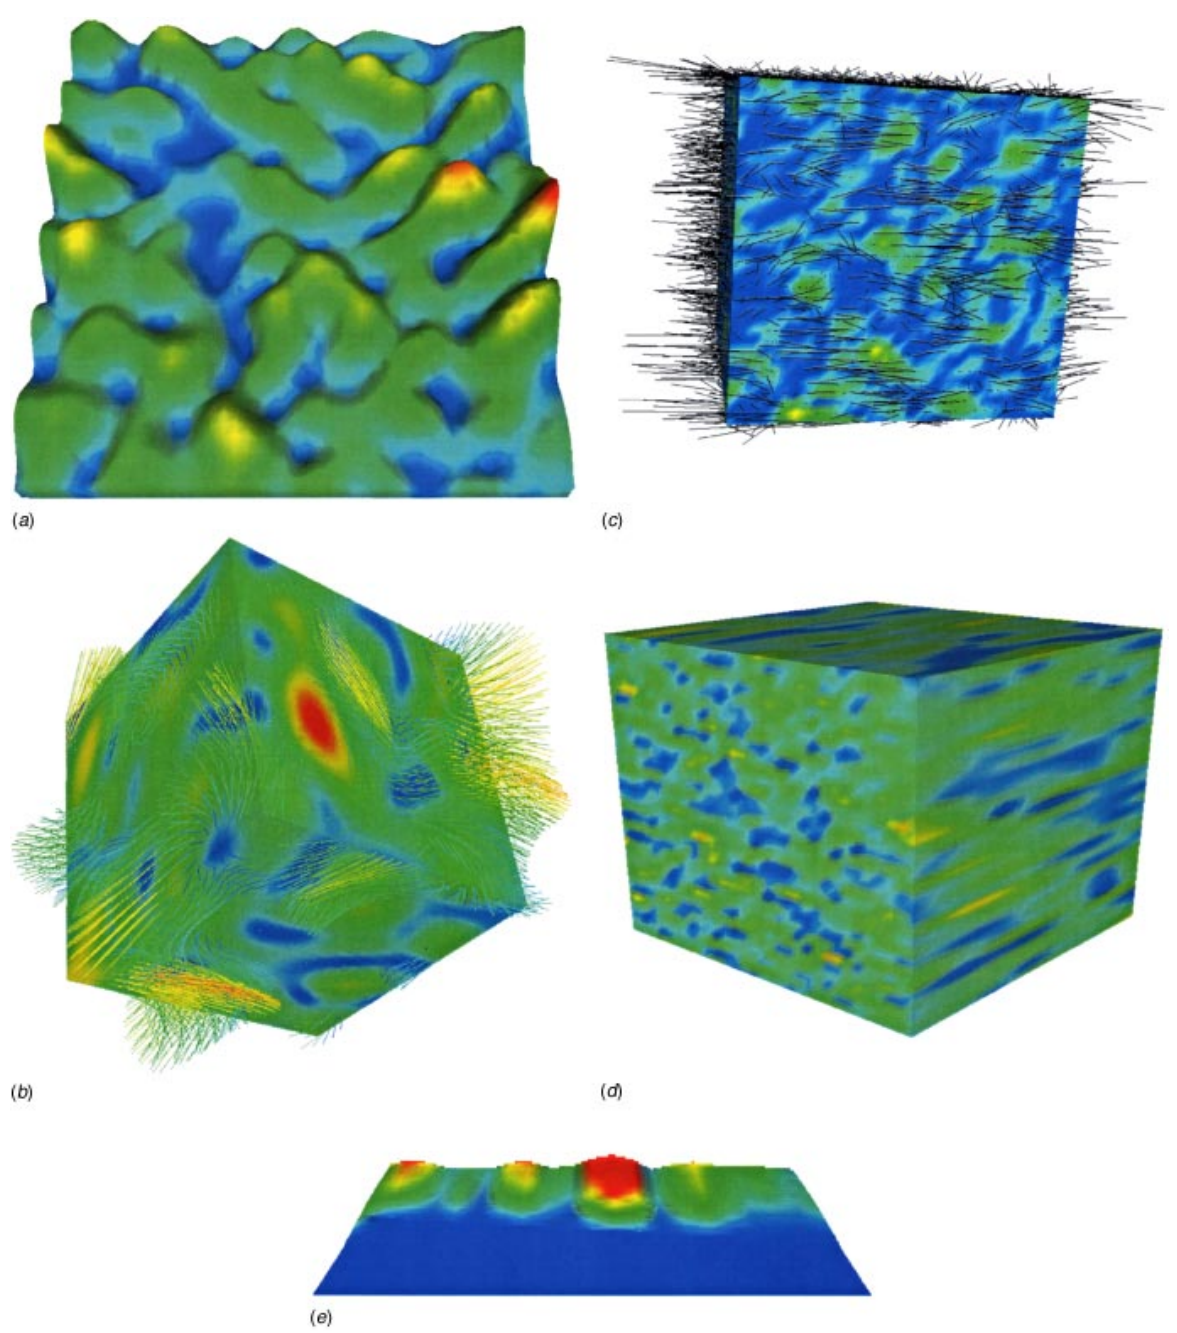
\includegraphics [width=0.6\linewidth] {smirnov_feilds}
  \caption{Сгенерированные авторами поля скоростей для a) изотропная завихренность, b) изотропная скорость, c) анизотропная скорость d) анизотропный пространственный масштаб e) флуктуации на границе \cite{huang2010general}} 
  \label{img:smirnov_results}  
\end{figure}


\section{Метод Хуанга генерации синтетической турбулентности} \label{sect2_3}

Как упоминалось в секции \ref{sect2_2}, метод Смирнова задает базис для работы с генераций синтетической турбулентности. Как можно видеть, в методе присутствует достаточно большое число параметров. Эти параметры представляют собой, например, способ генерации случайных чисел, способ задания ряда Фурье, форма спектра, метод аппроксимации спектра, учет расстояний до стенок и тому подобное.
В методе используемым в статье~\cite{huang2010general} основное отличие заключается в используемом спектре. В методе Смирнова используется Гауссов спектр, который не так хорошо описывает реальный спектр при больших волновых числах, то-есть при приближении к интервалу диссипации. В работе Хуанга используется модифицированный спектр Вон-Кармана. Помимо этого используется специальный алгоритм аппроксимации спектра за счёт разложения его по базисным функциям. Однако вносимые в алгоритм правки, налагают дополнительные предположения, связанные с интегрируемостью флуктуации.

Ниже приведен график сравнения вида спектров используемых в работах Смирнова и Хуанга с близким к реальному спектром Вон-Кармана. Как можно видеть, в методе Смирнова спектр турбулентных флуктуаций не покрывает область больших волновых чисел. 

\begin{figure}[ht] 
  \center
  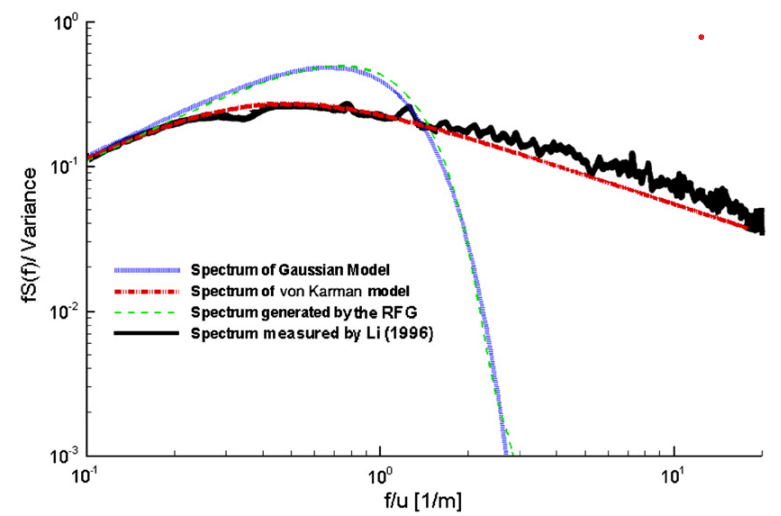
\includegraphics [] {huang_spect_rfg_smirnov_huang_li}
  \caption{Сравнение спектров для метода Смирнова со спектрами Вон-Кармана и спектром измеренным Ли\cite{huang2010general}} 
  \label{img:huang_spect_rfg_smirnov_huang_li}  
\end{figure}

На изображении \ref{img:huang_spect_rfg_smirnov_huang_li} показаны измерения для продольной компоненты флуктуации скорости потока ветра для процедуры генерации Смирнова с интенсивностью продольной турбулентности $I_u = 8 \%$ и интегральном масштабе турбулентности $L_u = 0.3 m$. Хорошо видно, что в области инерционного интервала для метода Смирнова наблюдается сильное затухание.

Как говорилось ранее, основная идея усовершенствования спектрального метода состоит в представлении целевого спектра в виде комбинации (суммы) небольших долей. Этот шаг можно назвать дополнительной дискретизации целевого спектра. За основу этих небольших долей берутся спектры, рассматриваемые нами ранее в работе Крайшнана \eqref{eq:spectral_equation2}. Авторы предлагают использовать для дискретизации спектры $E_1$ и $E_3$ для двумерного и трёхмерного случаев соответственно, в силу того, что они имеют ярко выраженный пик в значении $k = k_0$ и не влияют на другие "узлы" дискретизации. 

\begin{equation}
    \label{eq:spectral_equation14}
    E(k) = \sum_{m = k_0}^{k_{max}} E_m(k) = \sum_{m = k_0}^{k_{max}} E_m(k_m) \delta(k - k_m) = \sum_{m = k_0}^{k_{max}} \left( \frac{3}{2} v_m^2 \right) \delta(k - k_m)
\end{equation}

Теперь генерация, происходит для каждого слагаемого из суммы. Помимо этого, вводится явная зависимость между амплитудой получаемой скорости и значением энергии, соответствующее заданному волновому числу $k_m$. Стоит сразу отметить, что генерация поля скоростей для дискретизованного таким образом спектра, вносит дополнительную алгоритмическую сложность, в следствии необходимости дополнительных проходов генерации для каждого значения дискретизованного спектра. В этом случае флуктуация задается в виде:

\begin{equation}
    \label{eq:spectral_equation15}
    u_{m,i} = \sum_{n = 1}^{N} \left[ p_{i}^{m,n} \cos{(k_j^{m,n} \cdot x_j + \omega_n \cdot t)} 
        + q_{i}^{m,n} \cos{(k_j^{m,n} \cdot x_j + \omega_n \cdot t)}\right] 
\end{equation}
\noindent
здесь $k_i^{m,n}$ — изотропно распределенный вектор по сфере радиуса $k_m$, $\omega_{m, n} \in N(0, \omega_{m,n})$. Связывание амплитуд мод Фурье со значением спектра осуществляется по прямому определению значения $v_0$ — как среднеквадратичного отклонения скорости в любом направлении. Авторы выбирают следующее определение для нахождения связи:

\begin{equation}
    \label{eq:spectral_equation15_2}
    \sigma^2_{m,i} = \frac{1}{T} \int_{0}^{T} u_{m,i}^2 dt = \frac{2}{3} E_m(k_m) = \frac{2}{3} E(k_m) 
\end{equation}

В итоге получаем соотношение:
\begin{equation}
    \label{eq:spectral_equation15_3}
    \frac{1}{2} \sum_{n=1}^N \left[ p_i^{m,n} \right]^2 + \frac{1}{2} \sum_{n=1}^N \left[ q_i^{m,n} \right]^2 = \frac{2}{3} E(k_m) 
\end{equation}
Убедиться в этом можно прямой подстановкой \eqref{eq:spectral_equation15_2} в \eqref{eq:spectral_equation15}
\begin{align}
    & \frac{1}{T} \int_{0}^{T} u_{m,i}^2 dt = \nonumber \\ 
    & = \frac{1}{T} \int_{0}^{T} \left\{ \sum_{n = 1}^{N} \left[ p_{i}^{m,n} \cos{(k_j^{m,n} \cdot x_j + \omega_n \cdot t)} + q_{i}^{m,n} \cos{(k_j^{m,n} \cdot x_j + \omega_n \cdot t)}\right]  \right\}^2 dt                                                                          \nonumber \\
    & = \frac{1}{T} \sum_{n = 1}^{N} \left[p_i^{m,n}\right]^2 \frac{T}{2} + \frac{1}{T} \sum_{n = 1}^{N} \left[p_i^{m,n}\right]^2 \frac{T}{2} = \frac{1}{2} \sum_{n=1}^N \left[ p_i^{m,n} \right]^2 + \frac{1}{2} \sum_{n=1}^N \left[ q_i^{m,n} \right]^2 = \frac{2}{3} E(k_m)
\end{align}

Из вывода данной связи между значением энергии и мод Фурье вытекает, ранее упомянутое, требование к интегрируемости. В конечном итоге имеем в векторном виде следующие выражение:

\begin{equation}
    \label{eq:spectral_equation16}
    \frac{1}{2} \sum_{n}^N |\vec{p^{m,n}}|^2 + \frac{1}{2} \sum_{n}^N |\vec{q^{m,n}}|^2 = 2 E(k_m)
\end{equation}
\noindent
здесь записана система уравнений, связывающая амплитуды мод Фурье со значениями спектра для различных волновых чисел. Решать, данную систему можно различными способами. Первый наиболее очевидный способ использовать алгоритмы решения СЛАУ, но авторы поступили другим путём. Вводится дополнительная случайная величина $a$, через которую выражаются данные амплитуды. Это позволяет существенно сэкономить на решении СЛАУ, за счёт введения простой зависимости, а именно:

\begin{align}
    \label{eq:spectral_equation16_2}
    \vec{|p^{m,n}|} & = \sqrt{a \frac{4 E(k_m)}{N}} \nonumber \\
    \vec{|q^{m,n}|} & = \sqrt{(1 - a) \frac{4 E(k_m)}{N}}
\end{align}

Легко убедиться в том что данное выражение удовлетворяет уравнению \eqref{eq:spectral_equation16}, используя прямую подстановку:
\begin{equation}
    \frac{1}{2} \sum_{n}^N \vec{|p^{m,n}|}^2 + \frac{1}{2} \sum_{n}^N \vec{|q^{m,n}|}^2 = \frac{1}{2} \frac{4 E(k_m)}{N} \left[ 
    \sum_n^N a + \sum_n^N (1 - a) \right] = 2 E(k_m)
\end{equation}

Таким образом амплитуды мод Фурье, выражаются в виде:
\begin{equation}
    \label{eq:spectral_equation17_1}
    |\vec{p^{m,n}}| = \frac{\zeta \times \vec{k^{m,n}}}{|\zeta \times \vec{k^{m,n}}|} \sqrt{a \frac{4 E(k_m)}{N}}
\end{equation}
\begin{equation}
    \label{eq:spectral_equation17_2}
    |\vec{q^{m,n}}| = \frac{\zeta \times \vec{k^{m,n}}}{|\zeta \times \vec{k^{m,n}}|} \sqrt{(1 - a) \frac{4 E(k_m)}{N}}
\end{equation}

Авторы отмечают, что подход также требует корректировки значения пространственного масштаба турбулентности. Так как на самом деле оператор пространственной корреляции имеет зависимость от данного параметра:

\begin{equation}
    \label{eq:spectral_equation17}
    R(\vec x, \vec x') = \int_0^T \vec{u}(\vec x, t) \cdot \vec{u}(\vec x', t) dt \\
    = \sum_{m=k_0}^{k_{max}} \left\{ \frac{2 T E(k_m)}{N} \sum_{n=1}^N \cos{\left( \Tilde{\vec k}^{m,n} 
    \frac{\vec x - \vec x'}{L_s} \right)} \right\}
\end{equation}

Авторы предлагают, также, несколько иной подход к генерации анизотропной турбулентности, за счёт того, что имеется возможность разделить спектр на составляющие не только пространственно по-волновому вектора, но также и по компонентно. Разделим \eqref{eq:spectral_equation16} по компонентно в следующем виде:

\begin{equation}
    \label{eq:spectral_equation18}
    \frac{1}{2} \sum_{n}^N |\vec{p^{m,n}}|^2 + \frac{1}{2} \sum_{n}^N |\vec{q^{m,n}}|^2 = \frac{4}{3 N} E(k_m) = \frac{4}{N} E_i(k_m) 
\end{equation}

Как и до этого, введение случайного параметра по типу $a$, можно найти аналитическое выражение для задания амплитуд мод Фурье.

\begin{equation}
    \label{eq:spectral_equation18_1}
    p^{m,n}_i = \text{sign}(r_i^{m,n}) \sqrt{\frac{4}{N} E_i(k_m) \frac{(r_i^{m,n})^2}{1 + (r_i^{m,n})^2}}
\end{equation}
\begin{equation}
    \label{eq:spectral_equation18_2}
    q^{m,n}_i = \text{sign}(r_i^{m,n}) \sqrt{\frac{4}{N} E_i(k_m) \frac{1}{1 + (r_i^{m,n})^2}}
\end{equation}

Эта же процедура может использоваться и для генерации однородного поля скоростей путем задания одинакового спектра по всем пространственным направлениям. Стоит отметить, что с использованием матричных преобразований в методе Смирнова необходимо было, чтобы коэффициенты плавно менялись в пространстве для пренебрежения членами с их пространственными производными для удовлетворения уравнению неразрывности для случая генерации неоднородной и анизотропной турбулентности. В данном же случае, никаких подобных допущений не требуется, в результате чего уравнение неразрывности выполняется в точности.  

На валидации, авторам алгоритма удалось получить достаточно хорошее совпадение с целевым спектром. На рисунке ниже приведены результаты полученные авторами для трёх компонент флуктуаций скорости в сравнении со спектром Вон-Кармана. Параметры генерации те же, что использовались для сравнения для случая \ref{img:huang_spect_rfg_smirnov_huang_li}.

\begin{figure}[ht] 
  \center
  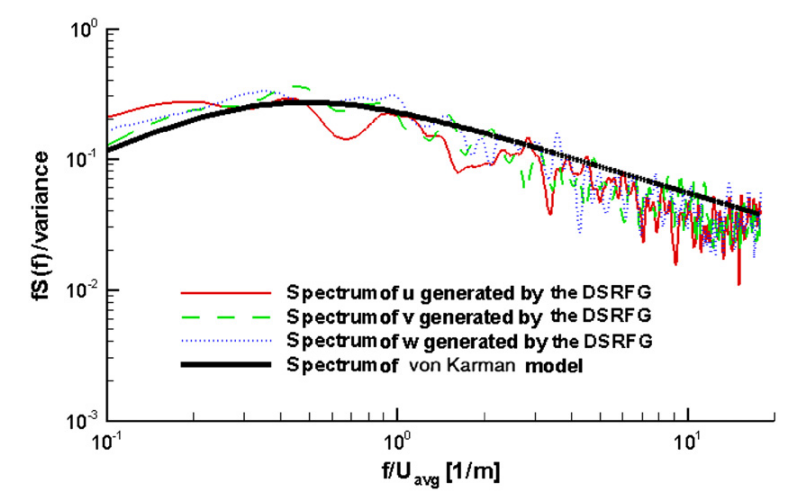
\includegraphics [] {huang_spect__huang_uvw}
  \caption{Сравнение результирующих спектров для сгенерированных компонент флуктуаций $u, v, w$ со спектром Вон-Кармана\cite{huang2010general}} 
  \label{img:huang_spect__huang_uvw}  
\end{figure}

\section{Метод Шура генерации синтетической турбулентности} \label{sect2_4}

Как упоминалось ранее, возможностей для изменения и корректировки метода открыто множество параметров. Один из них, внесение правок в сам алгоритм. Так в работе \cite{shur2014synthetic} вместо предложенным Смирновым ортогональных преобразований, используется разложение Холецкого для тензора напряжений Рейнольдса. Суть разложения Холецкого состоит в том, чтобы представить матрицу в виде произведения нижне треугольных матриц: $\hat{R} = \hat{A}^T \cdot \hat{A}$. Для прикладного случая - разложения тензора напряжений Рейнольдса, матрица $\hat{A}$ имеет вид:

\begin{equation}
    \label{eq:spectral_equation18_3}
     \hat{A} = a_{ij} = \begin{pmatrix}
                            \sqrt{R_{11}} & 0 & 0 \\
                            R_{21} / a_{11} & \sqrt{R_{22} - a_{21}^2} & 0 \\
                            R_{31} / a_{11} & \frac{R_{32} - a_{21} \cdot a_{31}}{a_22} & \sqrt{R_{33} - a_{31}^2 - a_{32}^2}
                        \end{pmatrix}
\end{equation}

Искомые флуктуации имеют вид:
\begin{equation}
    \label{eq:spectral_equation19}
    u_i(\vec r, t) = a_{ij} v_j(\vec r, t),
\end{equation}
\noindent
где $v_j$ - компоненты генерируемы по принципу \eqref{eq:spectral_equation1}, но также налагая требование $<v_i v_j> = \delta_{ij}$. В общем случае, разложение $\hat{R} = \hat{A}^T \cdot \hat{A}$ не является однозадачным, например можно также использовать разложение на собственные числа и значения $\hat{R} = \hat{A}^T \cdot \hat{C} \cdot \hat{A} = \hat{A}^T \cdot \hat{C}^{\frac{1}{2}} \cdot \hat{C}^{\frac{1}{2}} \cdot \hat{A} = \hat{B}^T \cdot \hat{B}$, но для данного случая, необходимо чтобы собственные значениям были больше 0, или в более общем смысле, изначальная матрица положительно определена. Основная проблема в том что, в общем случае, матрица корреляций не отрицательно определена, и вполне могут быть встречены отрицательные собственные числа. 

Докажем то, что приводимое разложение действительно задает корреляцию наперед, пусть целевая матрица корреляций $R$, и случайная величина $\zeta \in N(0, 1)$. Результирующая случайная величина $\xi = \hat{A} \cdot \zeta$. 
\begin{equation}
    \label{eq:spectral_equation19_1}
    \mathbb{E} \left(\xi \xi^T\right) = \mathbb{E} \left((\hat{A} \zeta)(\hat{A} \zeta)^T \right) = \mathbb{E} \left(\hat{A} \zeta \zeta^T \hat{A}^T\right) = \hat{A} \mathbb{E} \left(\zeta \zeta^T \right) \hat{A}^T = \hat{A} \hat{A}^T = R
\end{equation}
Помимо использования другого метода получения анизотропной турбулентности, авторы также используют несколько изменённое определение для генерации флуктуации. 
\begin{equation}
    \label{eq:spectral_equation20}
    \vec{v}(\vec r, t) = 2 \sqrt{\dfrac{3}{2}} \sum_{n=1}^N \sqrt{q_n} \left[ \sigma^n \cos{(k^n \vec{d}^n \cdot 
    \vec r + \phi^n)} \right]
\end{equation}
здесь $N$ - число мод Фурье, $q^n$ - нормированная амплитуда моды фурье, $k^n$ - амплитуда волнового вектора, $d^n$ - случайно распределённый на единичной сфере вектор, $k^n = k^n \vec d^n$ ($\vec \sigma^n \cdot \vec d^n$). 

Принцип остается тот же, за исключением того, что зависимость от времени явно исключается из алгоритма. Таким образом авторы определяют все случайные величины всего один раз, так они не включают зависимость от времени, а также существенно упрощают алгоритм. При исключении явного рассмотрения времени из формул, необходимо каким-либо образом учесть нестационарность турбулентности. Чтобы учесть временную зависимость, авторы используют волновую конвекцию, вводится учёт волновой конвекции через компоненты псевдовектора положения $r'$.

\begin{equation}
    \label{eq:spectral_equation21}
    \vec r' = \left\{ \frac{2 \pi}{k^n \max{(l_e(\vec r)}} (x - U_0 t), y', z'\right\}
\end{equation}

здесь $U_0$ -макромасштабная величина скорости, $l_e$ -локальный пространственный масштаб вихрей.

Авторы также используют свою связь между амплитудами дискретизованного спектра и амплитудами мод Фурье.

\begin{equation}
    \label{eq:spectral_equation21_2}
    q^n = \frac{E(k_n) \Delta k^n}{\sum_{n=1}^N E(k_n) \Delta k^n}
\end{equation}

Это выражение удовлетворяют требованию нормированность амплитуд мод Фурье, а также в сравнении с \ref{sect2_3} имеет более простую форму, без введения дополнительных случайных параметров.

Как отмечалось ранее, в работе также используется спектр Вон-Кармана.

\begin{equation}
    \label{eq:spectral_equation22}
    E(k) = \frac{(\frac{k}{k_e})^4}{(1 + 2.4 \frac{k}{k_e})^2) ^ {\frac{17}{6}}} f_{\eta} f_{cut} 
\end{equation}

\begin{equation}
    \label{eq:spectral_equation23}
    f_{\eta} = \exp{(-(\frac{12 k}{k_\eta})^2)} 
\end{equation}

\begin{equation}
    \label{eq:spectral_equation23_1}
    f_{cut} = \exp{\left(-\left[ \frac{4 \max{(k - 0.9 k_{cut}), 0}}{k_{cut}} \right]^3\right)},\\
    k_{cut} = \dfrac{2 \pi}{l_{cut}} 
\end{equation}
\noindent
здесь $k_e = \frac{2 \pi}{l_e}$ - волновое число отвечающее за наиболее энергосодержащую моду. За счёт введения зависимости от локальных масштабов требуется высокая точность его определения для получения физической турбулентности на более маленьких длинах её развития. Авторы предполагают, что определяется как: $l_e = \min{(2 d_w, C_l l_t)}$, $d_w$ - расстояние от точки до ближайшей стенки, $C_l = 3.0$ - эмпирическая константа, $l_t$ - масштаб фоновой модели RANS ($l_t = \frac{k_t^\frac{1}{2}}{C_\mu \omega_t}$ для  $k-\omega$ модели). Для фильтрующих функций выбираются следующие параметры: $l_\mu = (\frac{\nu^3}{\epsilon})^\frac{1}{4}$. В демпфирующей функции: $l_{cut} = 2 \min{(\max{(h_y, hz, 0.3 h_{max})} + 0.1 d_w, h_{max})}$, $h_y,h_z$ - это локальные шаги сетки на интерфейсе RANS-LES, а $h_{max}=\max{(h_x,h_y,h_z)}$.

Так как распределение волновых чисел фиксируется, авторы используют геометрический ряд, для уменьшения количества волновых чисел: $k^n = k^{min}(1 + \alpha)^{n -1}, 0.01 \leq \alpha \leq 0.05$. Здесь $k^{min} = \beta k^{min}_e$ - минимальное волновое число в наборе, $\beta = 0.5$ - эмпирическая константа, $k^{min}_e$ - волновое число, соответствующее максимальному значению $l_e$ на интерфейсе, $l_e^{max} = \max{(l_e(\vec r))}$, $N$ - минимальное целое число для которого $k^N \geq k^{max} = 1.5 \max{k_{cut}(\vec r)}$. 

Суммируя алгоритм приведённый выше, используется фиксированный набор волновых чисел, также фиксированный по времени, и варьируется от значения соответствующего наибольшей длине волны в рассматриваемой задаче, до предела Нейквиста. Также спектра определяющий нормированные амплитуды в каждой точке имеет максимум при локально определённых волновых числах $k_e(\vec r) =\dfrac{2 \pi}{l_e(\vec r)}$, то-есть движется по фиксированному набору волновых чисел так, что моды с наибольшей длиной волны масштабируются малыми амплитудами вблизи стен, с наименьшей длиной волны масштабируются на малые амплитуды вдали от стен. Комбинация этих свойств STG обеспечивает образование сильно анизотропных (удлиненных) вихрей вблизи стенок и почти изотропных вихрей вдали от стенок.

Также все случайные величины входящие в \eqref{eq:spectral_equation20} определяются всего один раз, нивелируя высокочастотные флуктуации способствующее затуханию или ламинаризации ниже по потоку.
           % Глава 2
%\chapter{Валидация спектрального метода генерации синтетической турбулентности} \label{chapt4}

Одним из важных аспектов данной работы является программирование приведенных в главах \ref{chapt1} и \ref{chapt2}. Помимо того, что для достижения основной цели работы необходимо провести множество вычислений, необходимо также провести оптимизации алгоритмов, как для дальнейшего использования, так и для возможной конкуренции на рынке вычислительных пакетов и алгоритмов. Поэтому нужно уделить большее внимание данному аспекту. Помимо программирования основных методов, необходимо также реализовать сопутствующий функционал для валидации алгоритмов, а также удобного предоставления данных. Процесс можно разбить на несколько этапов. Первоначально, необходимо выбрать язык программирования для реализации алгоритмов. Следующим этапом проработать архитектуру приложения. В конечном итоге проводить вычислительные эксперименты.

Для выбора языка программирования, на котором будет вестись разработка, будут играть ключевую роль скорость, а также более простая интеграция с другими программами или сервисами. По первому признаку лучше всего подходят компилируемые языки программирования, дающие возможность получить наибольшую производительность. Наиболее популярным открытым пакетом для вычислительной гидродинамики является пакет "OpenFOAM". Для интеграции с "OpenFOAM" и различными библиотеками, например, линейной алгебры, наиболее лучшим вариантом становится выбор языка C или C++. Первый является подмножеством второго, выбор падает на C++ в силу предоставляемых языком программирования и его библиотекой стандартных примитивов, а также возможность интеграции с приведёнными выше пакетами. 

Тестирование алгоритмов проводилось на машине со следующими характеристиками:

\begin{enumerate}
	\item Процессор: Intel Core i5-13600KF (20 потоков, $\sim$4.9 Ггц);
	\item RAM: Kingston Fury 4800 Мгц, 36-38-38-38;
	\item SSD накопитель: ADATA LEGEND 840 (чтение 5000 Мбайт/c, запись 3500 Мбайт/с);
\end{enumerate}

Компиляция программ для тестов и замеров производительности производилась с флагом максимальной оптимизации $\text{O3}$, без использования флага $\text{ffast-math}$ и подобных ему для ускорения работы с числами. Используемый тулчейн (ToolChain): $\text{LLVM}$ -- данная инфраструктура позволяет более бесшовно производить кросс компиляцию проекта для разным операционных систем и архитектур процессоров.

Помимо реализации алгоритмов, необходимо реализовать также функционал связанный с расчётами статистических параметров, а также функционала для работы с сетками и вычислительными областями. Также необходимо реализовать функционал связанный с сохранением полученных данных для их дальнейшей обработки, таким образом можно сэкономить на памяти при выполнении дампов текущих параметров и полей. 

На данном, начальном этапе, пока будем реализовать функционал без интеграции с другими CFD пакетами, так как эта интеграция пока не требуется для валидации алгоритмов.

Также решено было реализовать варианты генерации синтетической турбулентности в виде библиотек для простоты дальнейшего использования, предоставляя программный интерфейс для генерации синтетической турбулентности для будущего пользователя. 

%
% Постановка задачи
%
Задачей является сгенерировать поле флуктуаций. Для турбулентного поля скоростей можно вычислить большое количество характеризующих его параметров, на данный момент нас в большей степени интересует спектр турбулентных флуктуаций. Спектр является главным входным параметром генерации, вследствие чего, вычисление его для результирующего поля, полученного в результате генерации, является основным критерием для оценки того или иного метода насколько он хорош для использования в качестве генератора турбулентных флуктуаций. С самим же спектром, в свою очередь, связано также достаточно много параметров. Например, как было описано ранее в главах \ref{chapt1} и \ref{chapt2}, спектр имеет связь как с тензором спектра скоростей, так и с тензором ковариаций. Последний является важной статистической величиной для оценки пространственной зависимости (корреляции) величин. Таким образом мы добавляем ещё один критерий валидации к поставленной задаче. 

Основное сравнение для спектрального метода будем проводить в сравнении с целевым спектром, либо со спектрами, которые должны получаться в результате генерации, как в работе Крайшнана. Как говорилось ранее, проводилась реализация метода Крайшнана, так как он является базисом для построения модификаций и других методов. Помимо этого сразу есть возможность выявить недостатки или преимущества данного метода по сравнению с модификациями вносимыми другими авторами. 

Так как метод сразу нацелен на генерацию трёхмерного поля скоростей будем рассматривать сразу все компоненты флуктуаций и результирующего спектра. 

Для генерации турбулентных флуктуаций на основе спектральных методов необходимо выделить основные физические парамеры для дальнейшего их переноса в программный код. Таким образом мы выделяем структуры данных, необходимые для реализации алгоритма. Основные соотношения и формулы позволяют выделить алгоритмы над упомянутыми ранее структурами данных как образами над физическими величинами. В отличие от метода стохастического Гауссового моделирования здесь имеется больше пространства как в плане количества рассматриваемых величин, так и в плане объема требуемых алгоритмов. По примеру Хуанга мы можем разбить целевой спектр в ряд, также будем рассматривать генерацию поля скоростей для случаев \ref{eq:spectral_equation3} дельта функции и Гауссового спектра. Первый случай позволяет использовать нам генератор на основе метода Крайшнана для генерации во всём интересующем диапазоне волновых чисел, второй в свою очередь для простого использования генератора в интервалах генерации и инерционном. Мы хотим использовать данные спектры чтобы не уходить от оригинальной постановки задачи и как можно более близко оставаться в рамках изначальных условий. Для одного экземпляра генератора нам необходимо сгенерировать последовательность волновых векторов в соответствии с процедурой генерации для каждого из спектров, для случая спектра дельта функции волновые вектора генерируются статистически изотропно на сфере заданного радиуса $k_0$, для случая гауссова спектра используется нормальное распределение со среднеквадратичным отклонением $\dfrac{k}{2}$. Дальше необходимо задаться некоторым значением среднеквадратичного отклонения для частоты $\omega_0$. Основное влияние эта частота оказывает на временную зависимость генерации синтетической турбулентности. В целом, способов задаться этой частотой достаточно много, авторы предлагают использовать $\omega_0 = k_0 v_0$, $v_0$ -- среднеквадратичное отклонение в любом направлении. Как можно легко убедиться комплекс $k_0 v_0$ имеет размерность частоты, а также может использоваться для перехода к безразмерному времени. Остается сгенерировать лишь амплитуды мод фурье, в оригинальной работе авторы не специфицируют алгоритм генерации, а точнее параметры генерации, данной последовательности случайных векторов. Но важно, что вектора амплитуд мод Фурье генерируются из трёхмерного нормального распределения. В данной работе мы использовали вариант со средним равным 0 и матрицей ковариации заданной единичной матрицей. Набор этих случайных величин генерируется всего один раз на этапе инициализации генератора и никак не привязан в топологии сетки. Важно отметить, что мы будем использовать разные экземпляр генератора для проведения одной реализации поля скоростей в начальный момент времени для оценки спектральных и статистических характеристик. Для оценки временных характеристик используется один экземпляр генератора с заранее заданным шагом генерации по времени. 
Всё это дает нам возможность использовать подход Хуанга для генерации синтетического поля скоростей с идей дискретизации спектра, а также в будущем заложить другую информацию, например о тензоре Рейнольдса в матрицу ковариаций генератора. 

Генерация случайных чисел проводилась с использованием генераторов случайных чисел, предоставляемых стандартной библиотекой шаблонов языка C++, для генерации многомерного Гауссова распределения использовалась библиотека "Armadillo". Генератор псевдослучайных чисел базируется на алгоритме Вихрь Мерсенна, показывающий более лучшие спектральные свойства по сравнению с генераторами Кнута и минимальный стандартным механизмом \cite{l2002object}, механизм Вихря Мерсенна имеет высокую производительность и хорошее качество генерируемых случайных чисел. Скорость работы генераторов является важной характеристикой, так как рассматриваемые алгоритмы полностью базируются на случайных числах. Функции распределения используемые в работе также использовались из стандартной библиотеки шаблонов С++ и библиотеки "Armadillo". 

Для удобства дальнейшей обработки данных будем генерировать поля флуктуаций на кубической сетке. Длину куба в параметрах будет обозначать $l$ и, как для рассматриваемого в данной главе метода, так и для стохастического метода, будем брать $l = 10$, пока без введения конкретной размерности. Также сетка характеризуется числом разбиений по каждой из осей, будем использовать одинаковое число разбиений для каждой из осей $n_x = n_y = n_z = n$. Число разбиений будем использовать максимально доступное для вычислений на машине с объемом оперативной памяти в 32 Гб. Данный метод имеет хорошую устойчивость к топологии сетки, то-есть не зависит от расположения соседних узлов, её формы, поэтому можно с большой достоверностью считать, что использование данной сетки обосновано для проведения валидации получаемых данных. Для простоты также центр куба будет совпадать с началом координат, так будет проще оценить симметричность функций относительно точки расчёта статистических параметров, которую также примем за начало координат, в этом случае $R_{ij}(\vec x, \vec r) = \left< u_i(\vec x) u_j(\vec x + \vec r) \right> \rightarrow \left[ \vec x = {0, 0, 0} \right] \rightarrow R_{ij}(\vec r) = \left< u_i(\vec 0) u_j(\vec 0 + \vec r) \right>$. Важность оценки симметричности функции играет важную роль при переходе от тензора ковариаций к тензору спектра скоростей, так как это необходимое условие для проведения преобразования Фурье

Далее будут представлены сгенерированные поля в момент времени $t = 0$ для $k_0 = \frac{\pi}{3}$, $n = 31$, $v_0 = 1$, $\omega_0 = v_0 k_0 = 2 \pi$, для спектра в виде дельта-функции. Для проведения статистического анализа, а также дальнейшего вычисления тензора спектра скоростей и энергетического спектра генерируется $N_{samples} = 10000$, в 10 раз больше взятого числа мод Фурье, которое составляет $N = 1000$. 

\begin{figure}[!ht]
    \center{

        \subcaptionbox[List-of-Figures entry]{Полное сгенерированное поле\label{img:spectral_slice_veloctiy_field_full_cube}}
        {\includegraphics[width=0.45\linewidth]{images/spectral/spectral_n32_l10_f1000_k0pi3/full_velocity_field_cube_spectral.png}}%
        \hfill
        \subcaptionbox{плоскость $xy$, $z = 0$\label{img:spectral_slice_veloctiy_field_x_znormal_angle_trace}} 
        {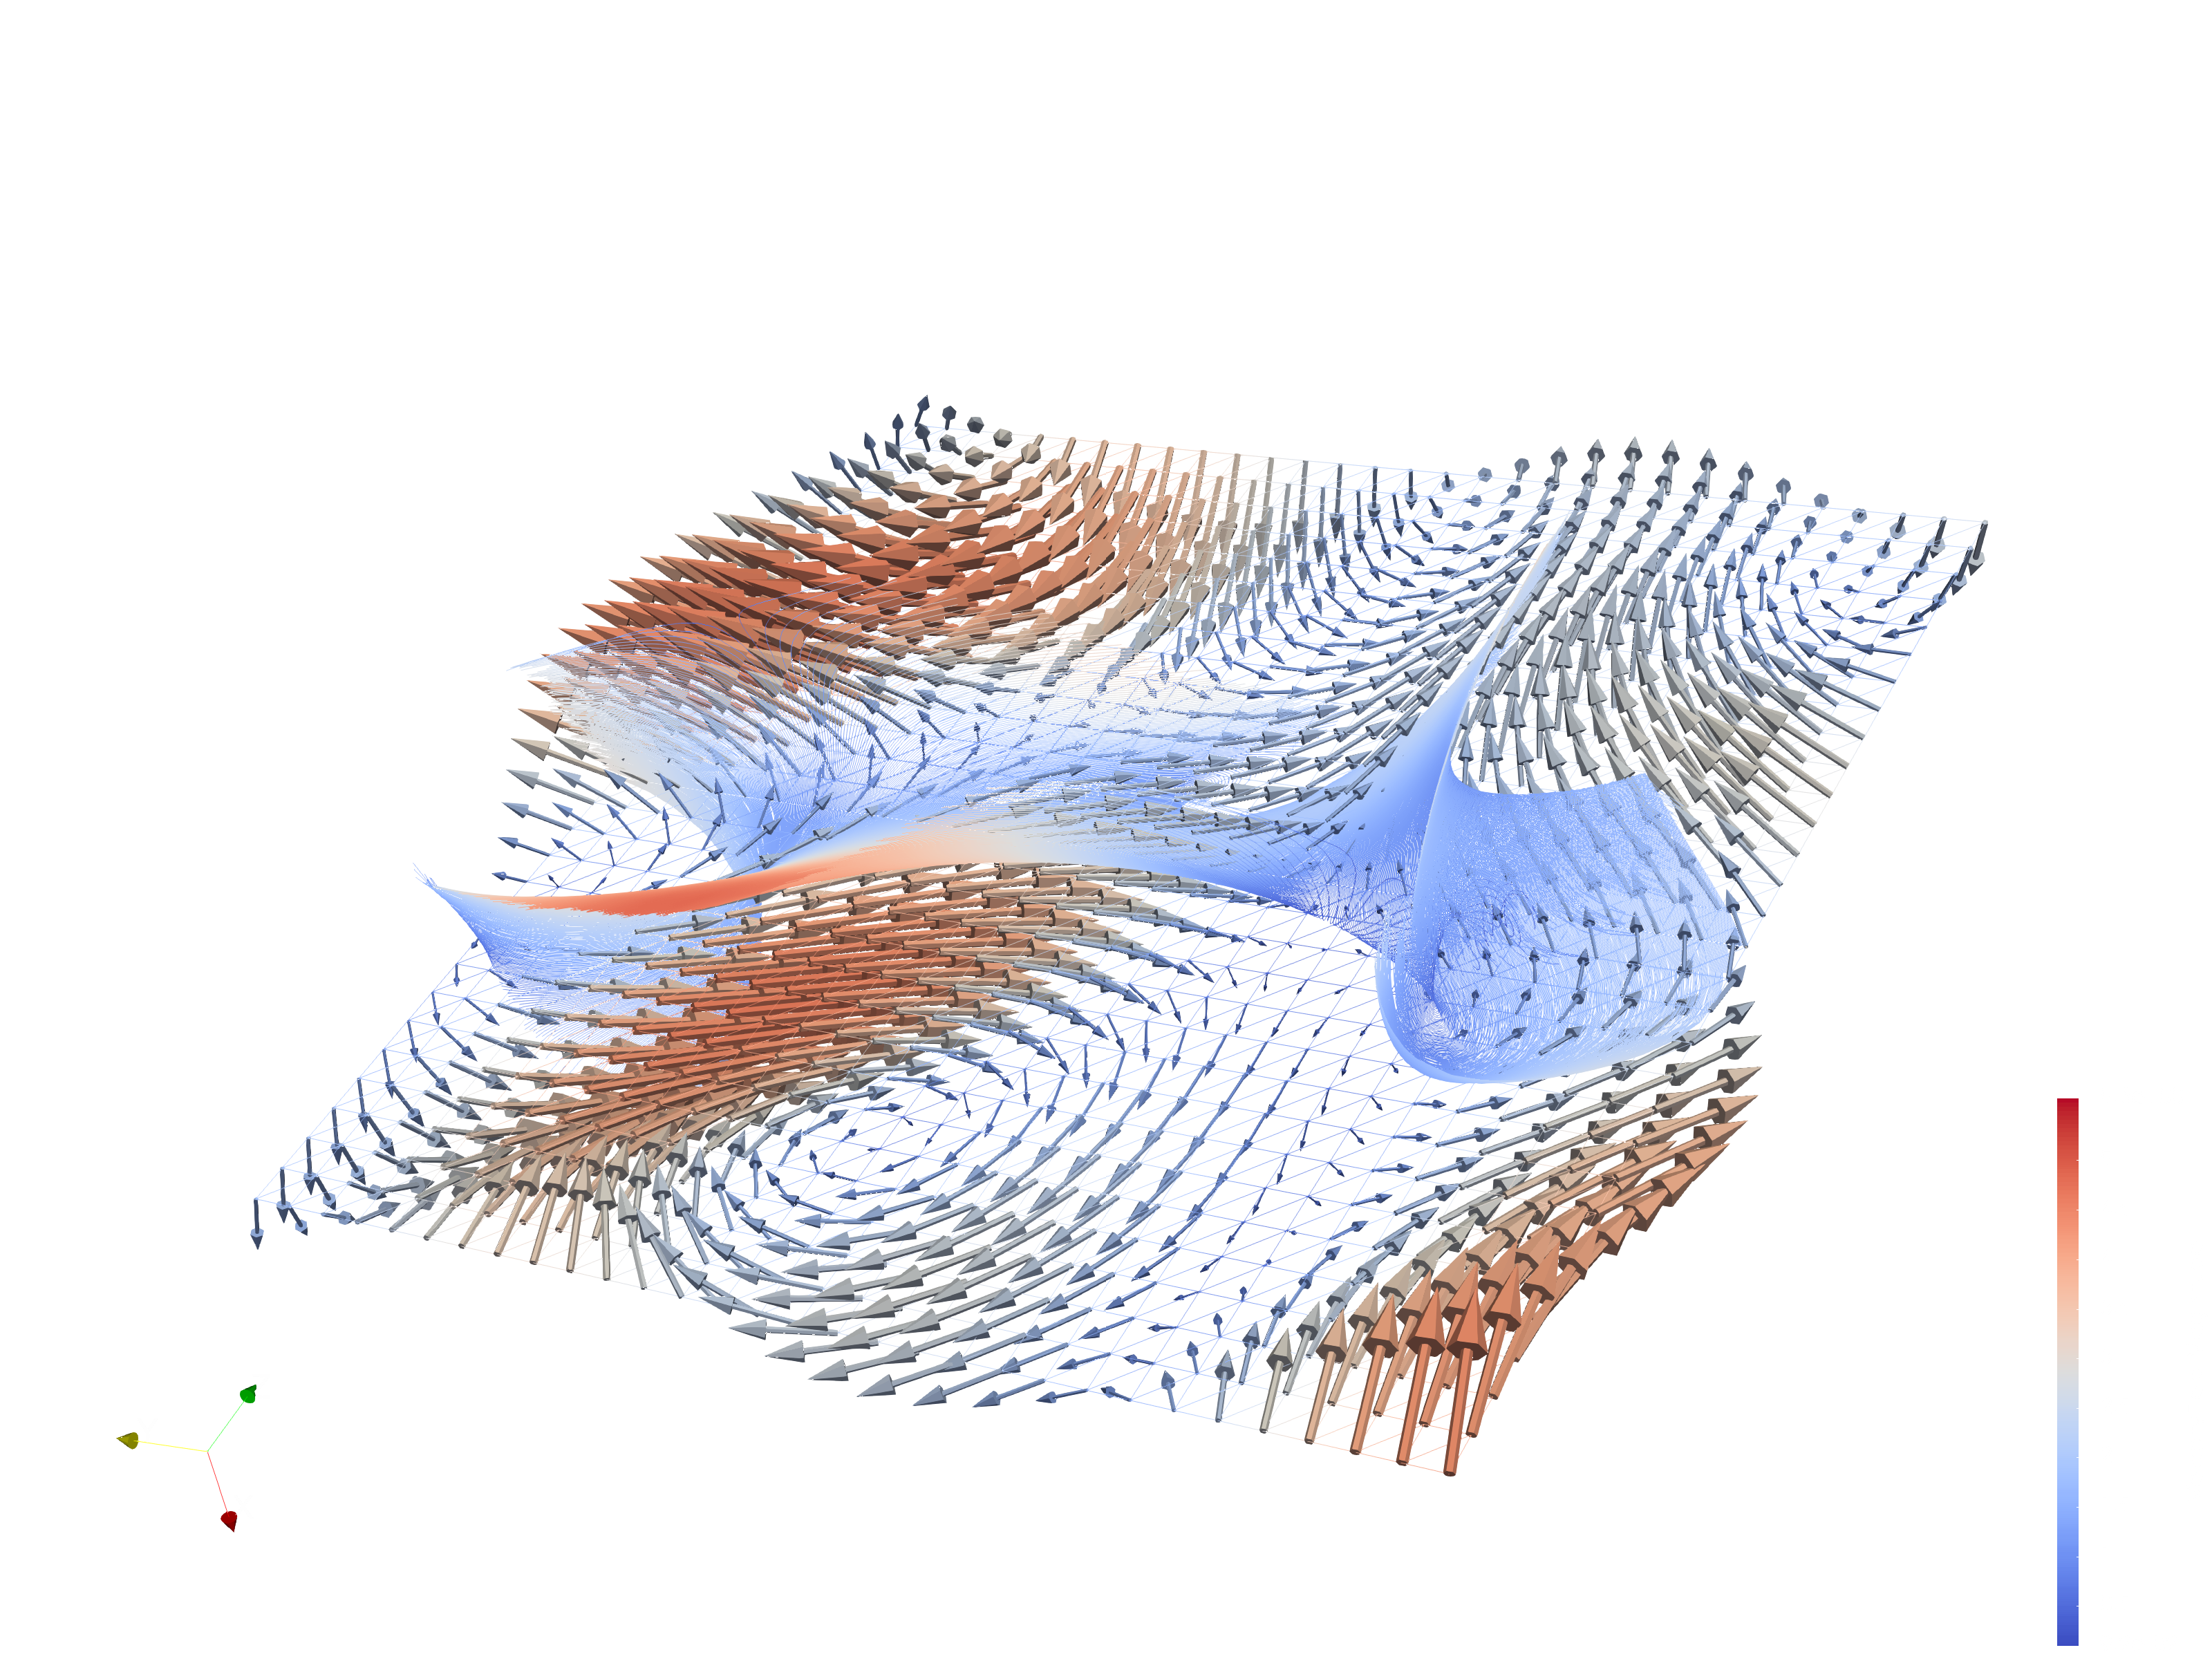
\includegraphics[width=0.45\linewidth]{images/spectral/spectral_n32_l10_f1000_k0pi3/spectral_x_normal_velocity_field_angle_trace.png}} \\
    }

    \center{
        \subcaptionbox[List-of-Figures entry]{плоскость $xy$, $z = 0$\label{img:spectral_slice_veloctiy_field_x_znormal_angle}} 
        {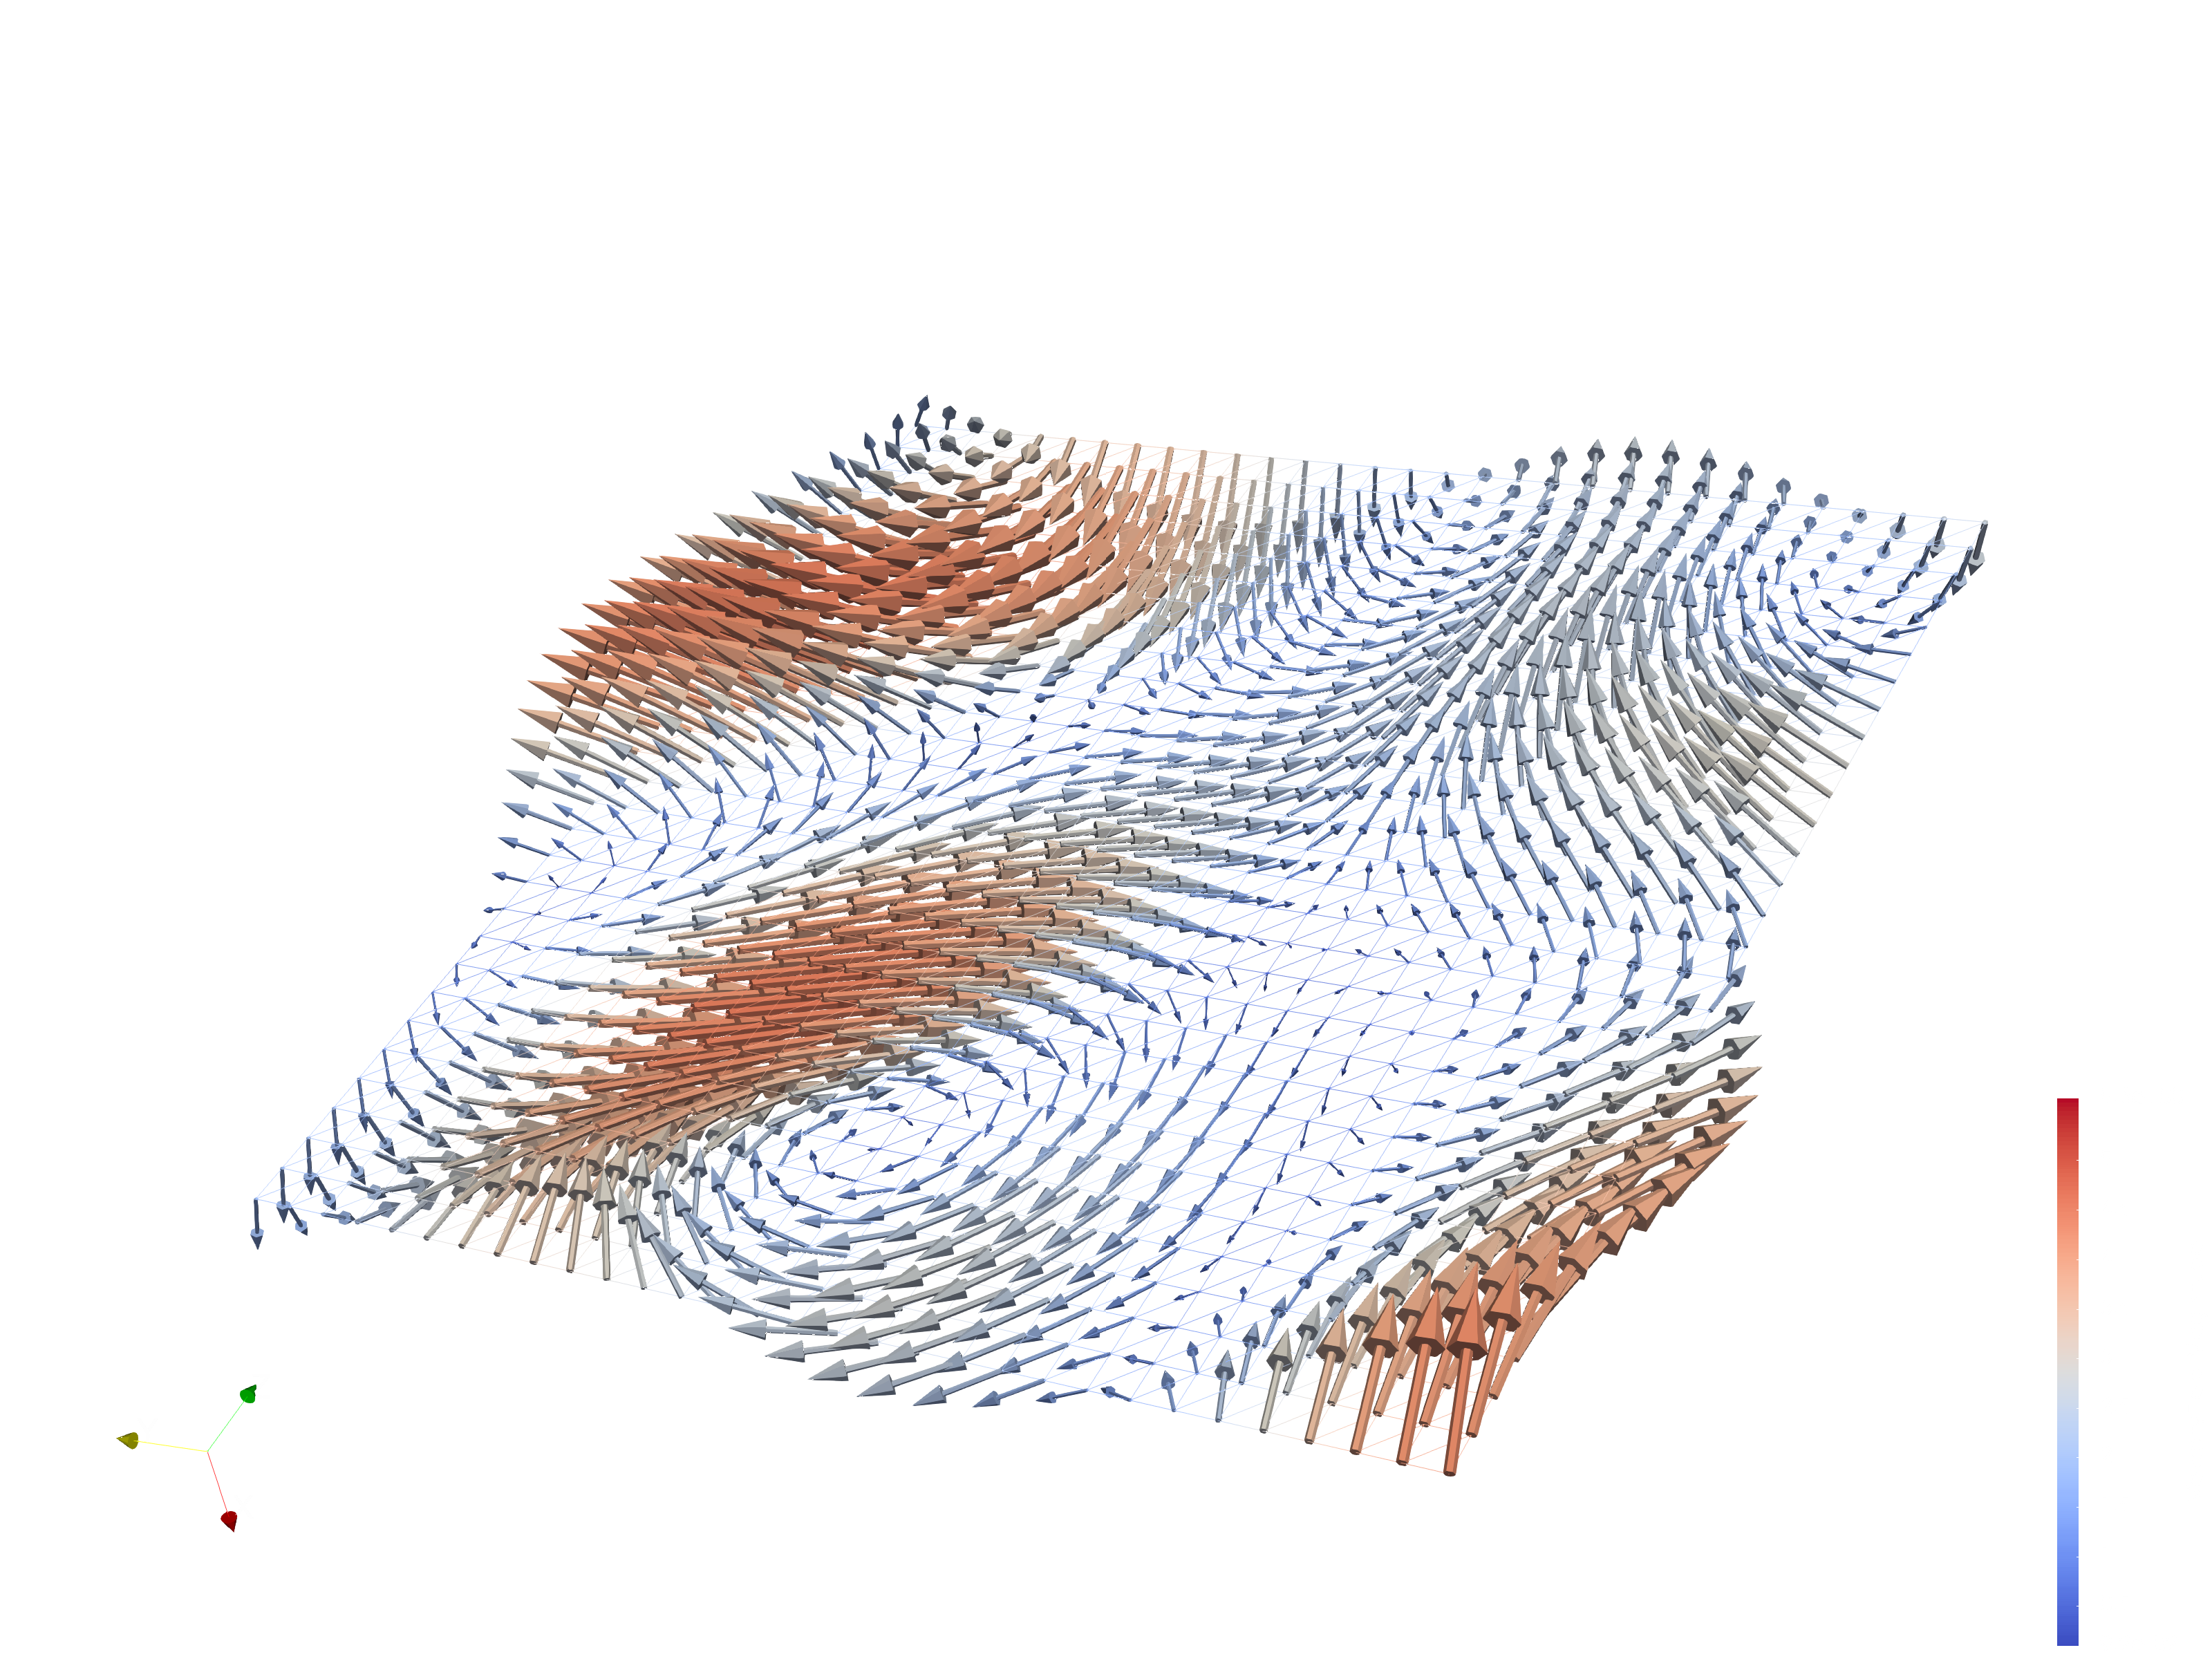
\includegraphics[width=0.45\linewidth]{images/spectral/spectral_n32_l10_f1000_k0pi3/spectral_x_normal_velocity_field_angle.png}}%
        \hfill
        \subcaptionbox{плоскость $xy$, $z = 0$\label{img:spectral_slice_veloctiy_field_x_znormal_no_angle}} 
        {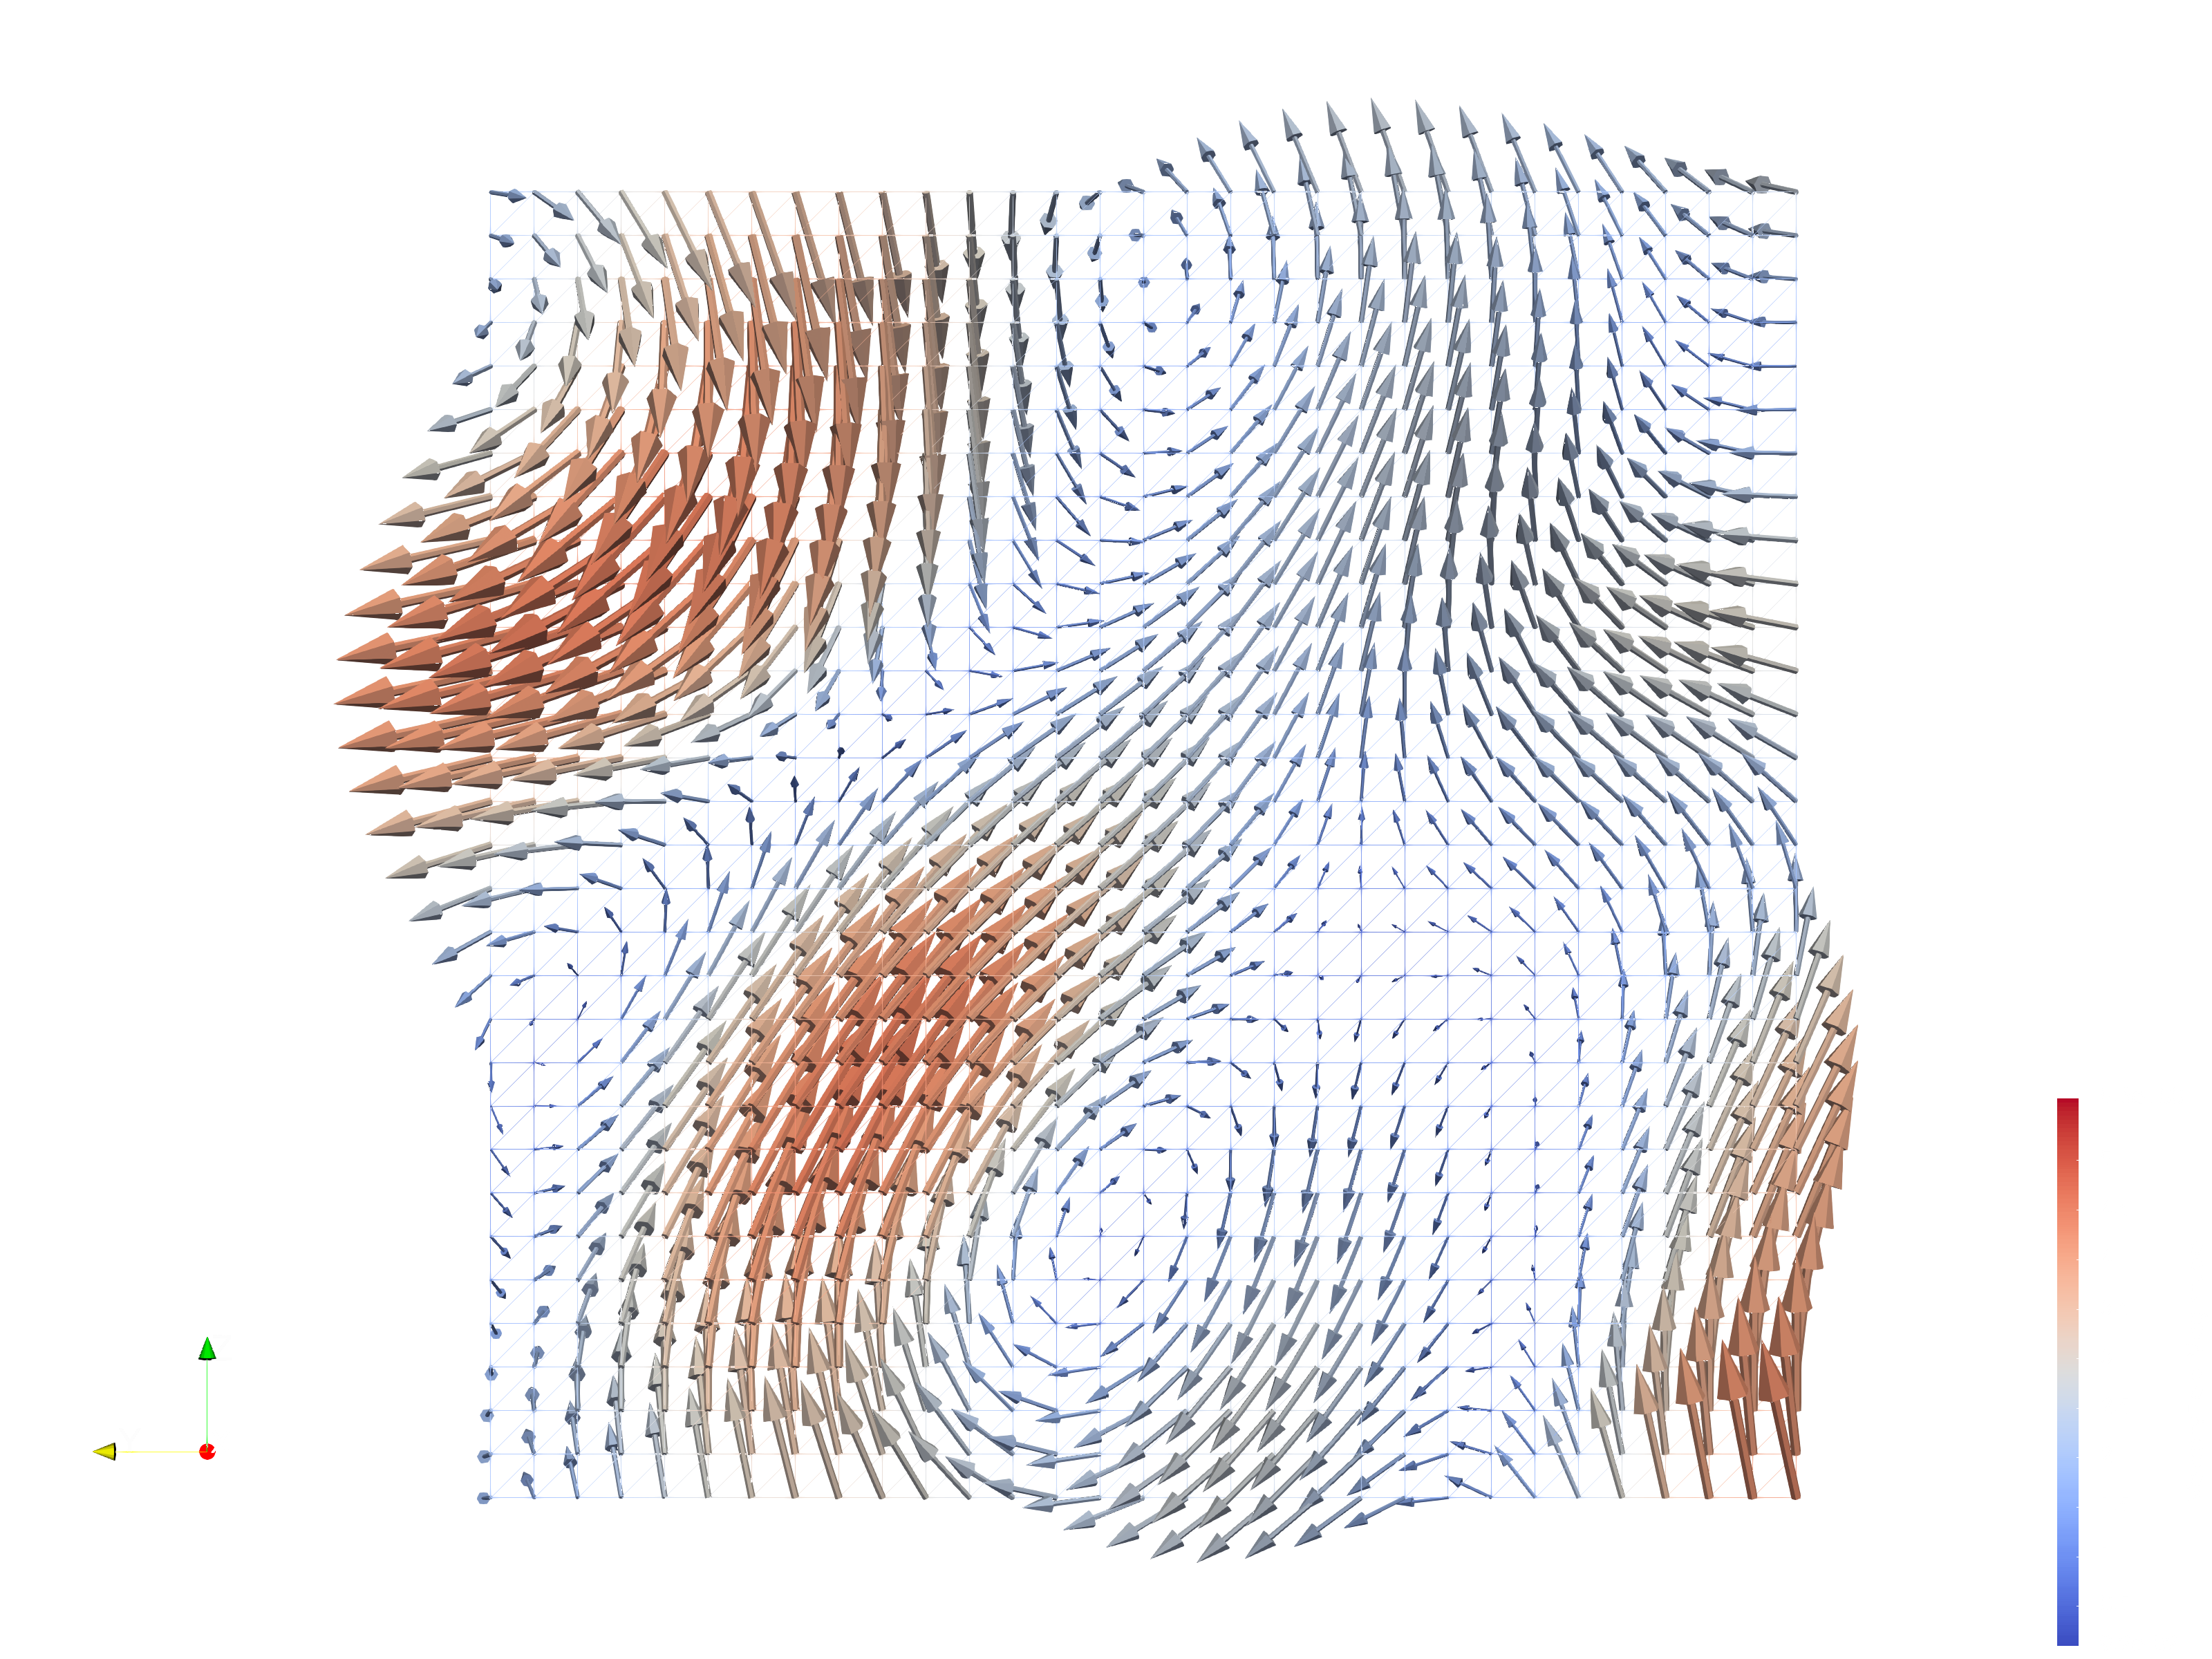
\includegraphics[width=0.45\linewidth]{images/spectral/spectral_n32_l10_f1000_k0pi3/spectral_x_normal_velocity_field.png}}
    }
    
    \onehalfspacing{Поле на картинке б представлено с линиями тока, расчитанными вдоль оси $y$}
    \caption{Поле флуктуаций сгенерированных трёхмерным стохастическим методом, цветом обозначена амплитуда флуктуаций}
    \label{img:velocity_fluctuation_field_for_spectral_1}  
\end{figure}

В отличие от стохастического метода, данный метод имеет явную зависимость вектора флуктуации от времени. Как говорилось выше, в данном случае распределение определяется сгенерированными частотами $\omega_0$. Мы можем выделить некоторый характерный период как $T = \frac{2 \pi}{\omega_0} = \frac{2 \pi}{k_0 v_0}$. Обычно при рассмотрении временных процессов берут период времени $100 T$, где $T = T_0$ -- характерный для задачи период (масштаб) времени. Шаг по времени выберем как $\Delta t = \frac{100 T_0}{N_{samples}}$ -- так мы можем трактовать поля сгенерированные во времени как одну реализацию поля флуктуаций. Ниже представлены сгенерированные поля для некоторых моментов времени. В общем случае, при данном шаге по времени наблюдается как плавный переход от одного поля к другому, так и достаточно резкий. Можно варьировать этот параметр путём задания среднеквадратичного отклонения для генерируемых частот -- $\omega_0$. Так для больших частот проявляется более частая смена ориентации векторов в пространстве.

%
%
% ТУТ КАРТИНКИ СГЕНЕРИРОВАННЫХ ПОЛЕЙ ВО ВРЕМЕНИ
%
%

На полученных реализациях мы можем оценить ковариационную функцию и последующими преобразованиями получить из неё и энергетический спектр. Ниже представлен рассчитанный на полученных реализациях тензор ковариаций относительно центра куба, совпадающего с началом координат, для различных направлений: по диагонали куба, по оси $x$, по оси $y$, по оси $z$, проходящие через начало координат. Различными цветами представлены компоненты тензора ковариаций. 

В случае однородной и изотропной турбулентности и несжимаемой жидкости есть возможность получить аналитическое выражение как для тензора ковариаций от функции энергетического спектра, так и для тензора спектра скорости от функции энергетического спектра \cite{Kraichnan70, pope2000turbulent}.

\begin{equation}
    \label{eq:part3_1}
    \left< \vec u (\vec x, t') \vec u (\vec x + \vec r, t) \right> = 2 D(t - t') \int_{0}^{\infty} E(k) \frac{\sin{(k r)}}{k r} dk 
\end{equation}

\begin{equation}
    \label{eq:part3_2}
    \Phi_{ij}(\vec k) = \frac{E(k)}{4 \pi k^2} \left( \delta_{ij} - \frac{k_i k_j}{k^2} \right)
\end{equation}

\noindent
здесь $k$ -- модуль волнового вектора, $k_i$ -- компонента волнового вектора.
Для обоих рассматриваемых методов генерация осуществляется в рамках однородной и изотропной турбулентности для несжимаемой жидкости, тем самым мы можем сравнить не только, например, спектральные характеристики, но и также провести сравнение других характеристик, таких как тензор ковариаций и тензора скоростей.

Рассмотрим полученные ковариационные функции на рассчитанные на 10000 реализаций поля флуктуаций с параметрами описанными выше.

\begin{figure}[!h]
    \center{

        \noindent \subcaptionbox[List-of-Figures entry]{диагональ куба\label{img:spectral_covariance_diagonal}} 
        {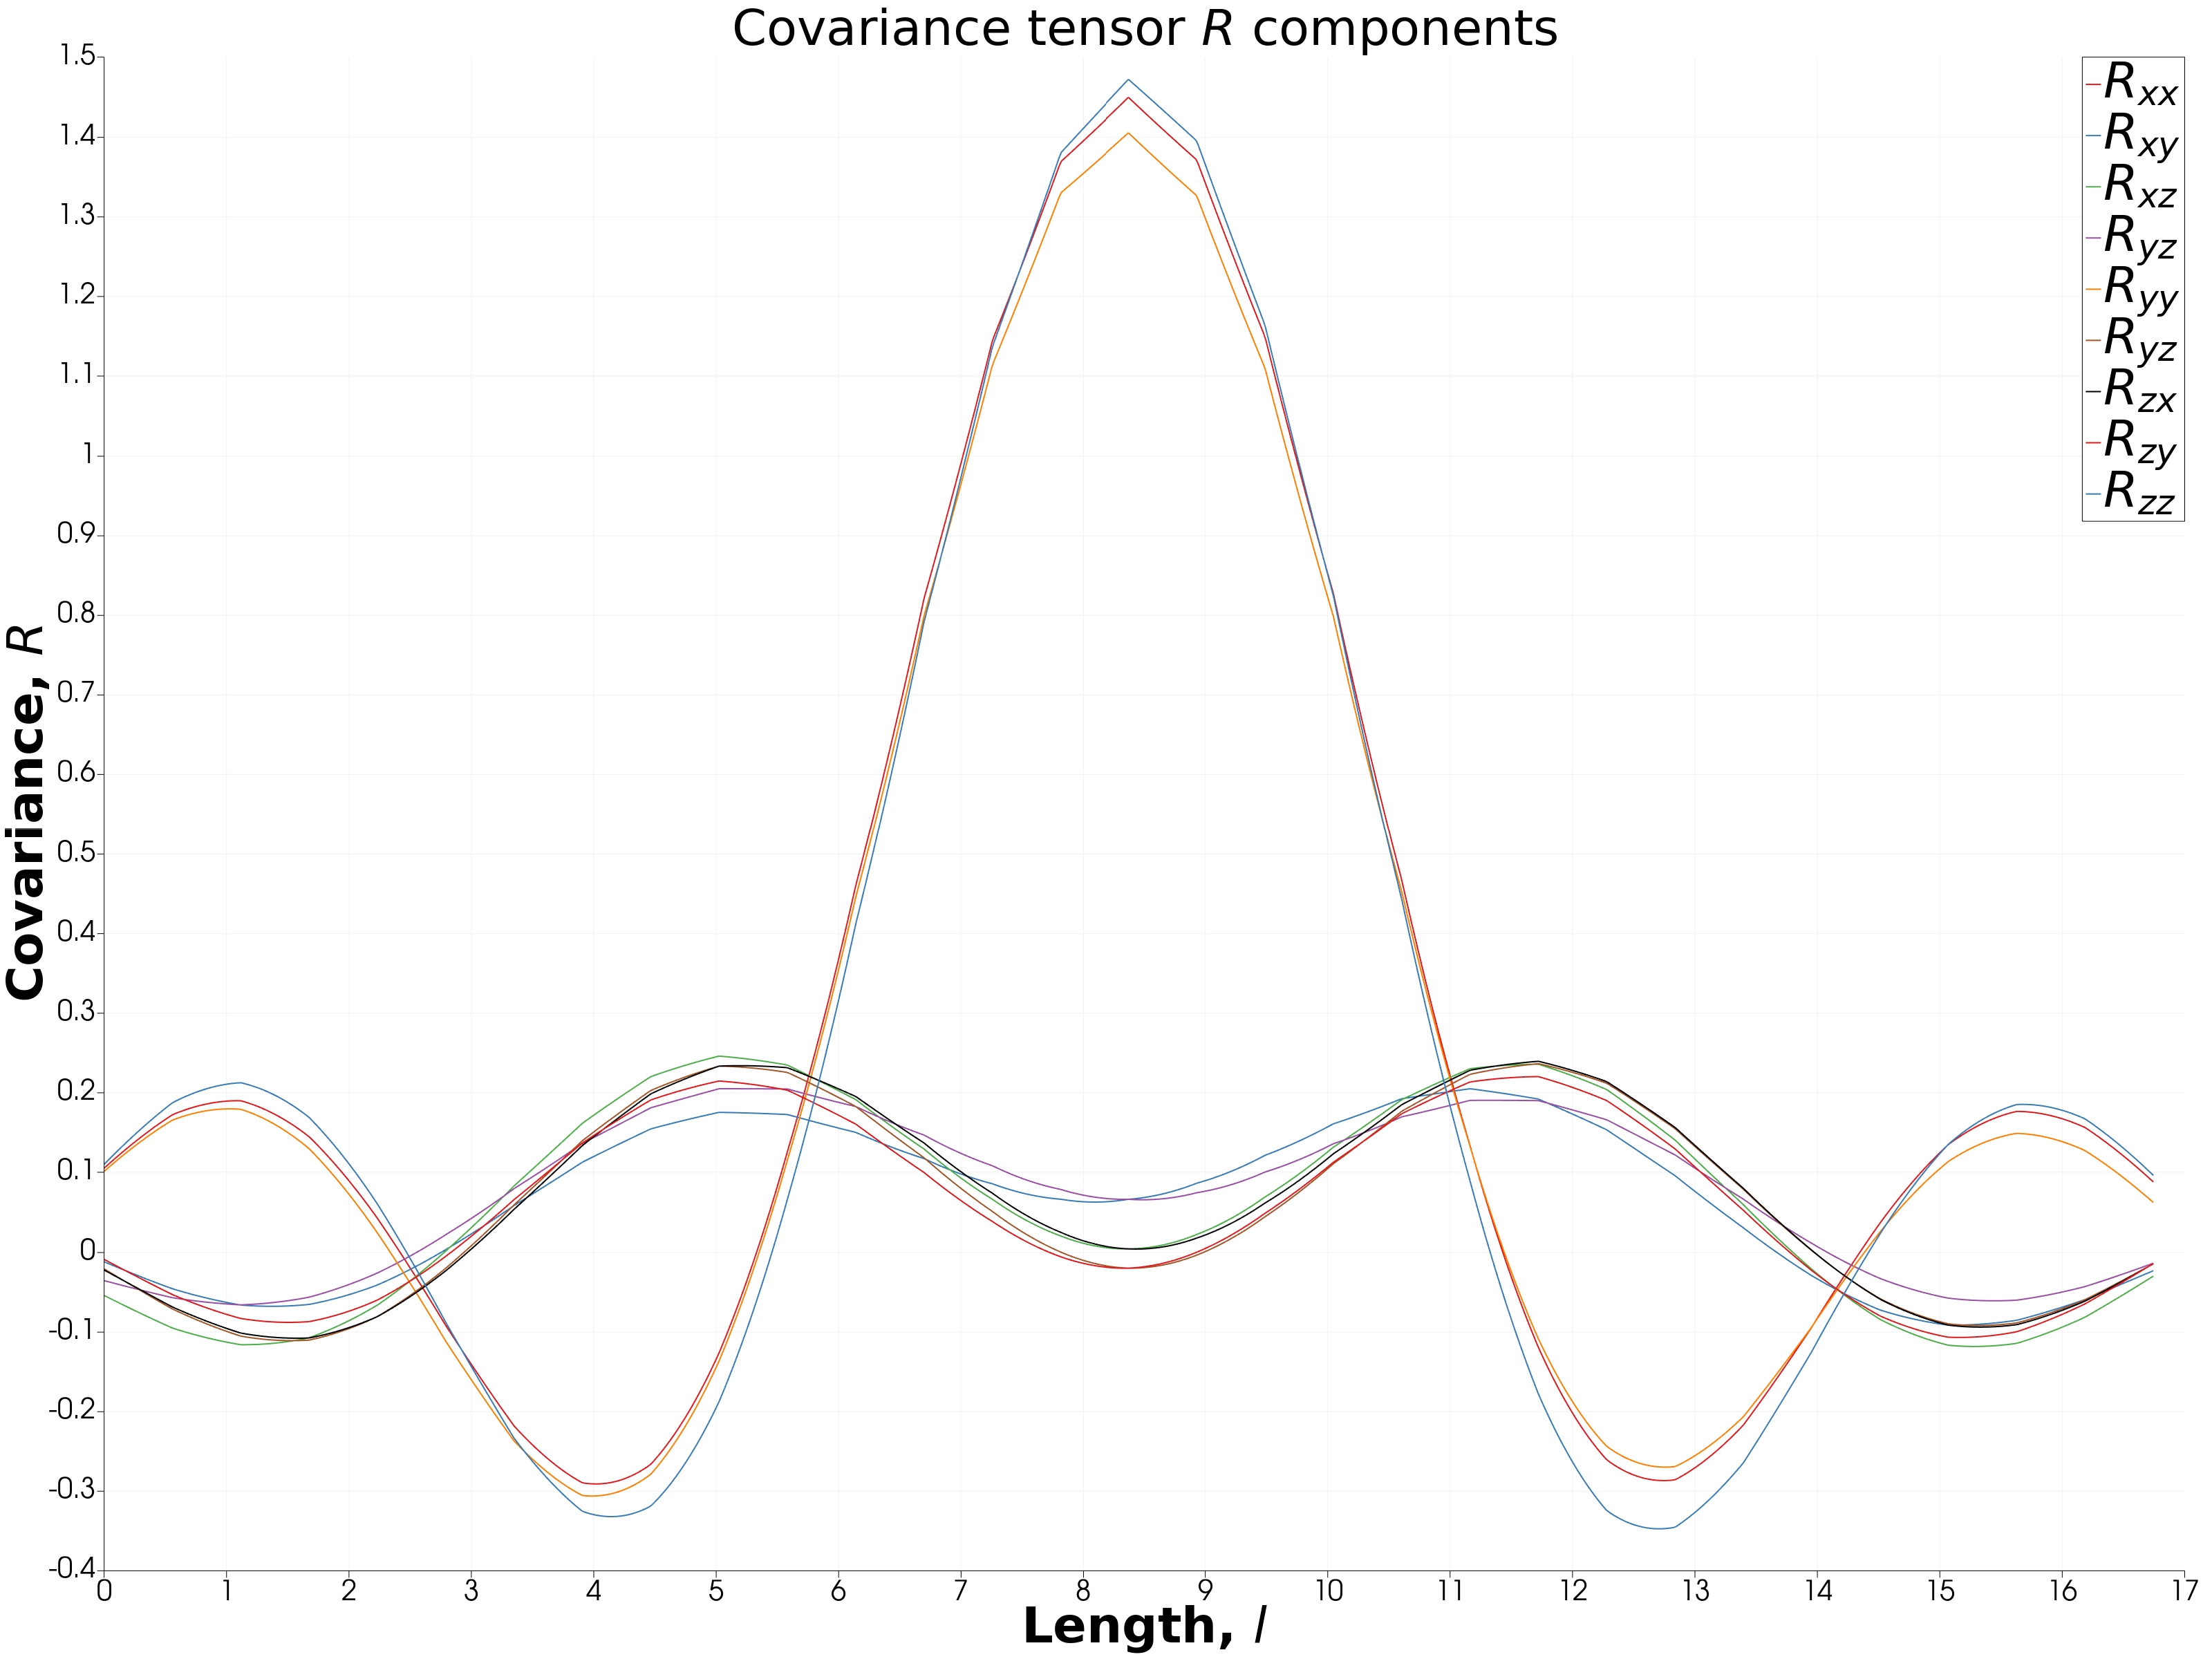
\includegraphics[width=0.45\linewidth]{images/spectral/spectral_n32_l10_f1000_k0pi3/covariance_function_diagonal.png}}%
        \hfill
        \subcaptionbox{$x$\label{img:spectral_covariance_x}} 
        {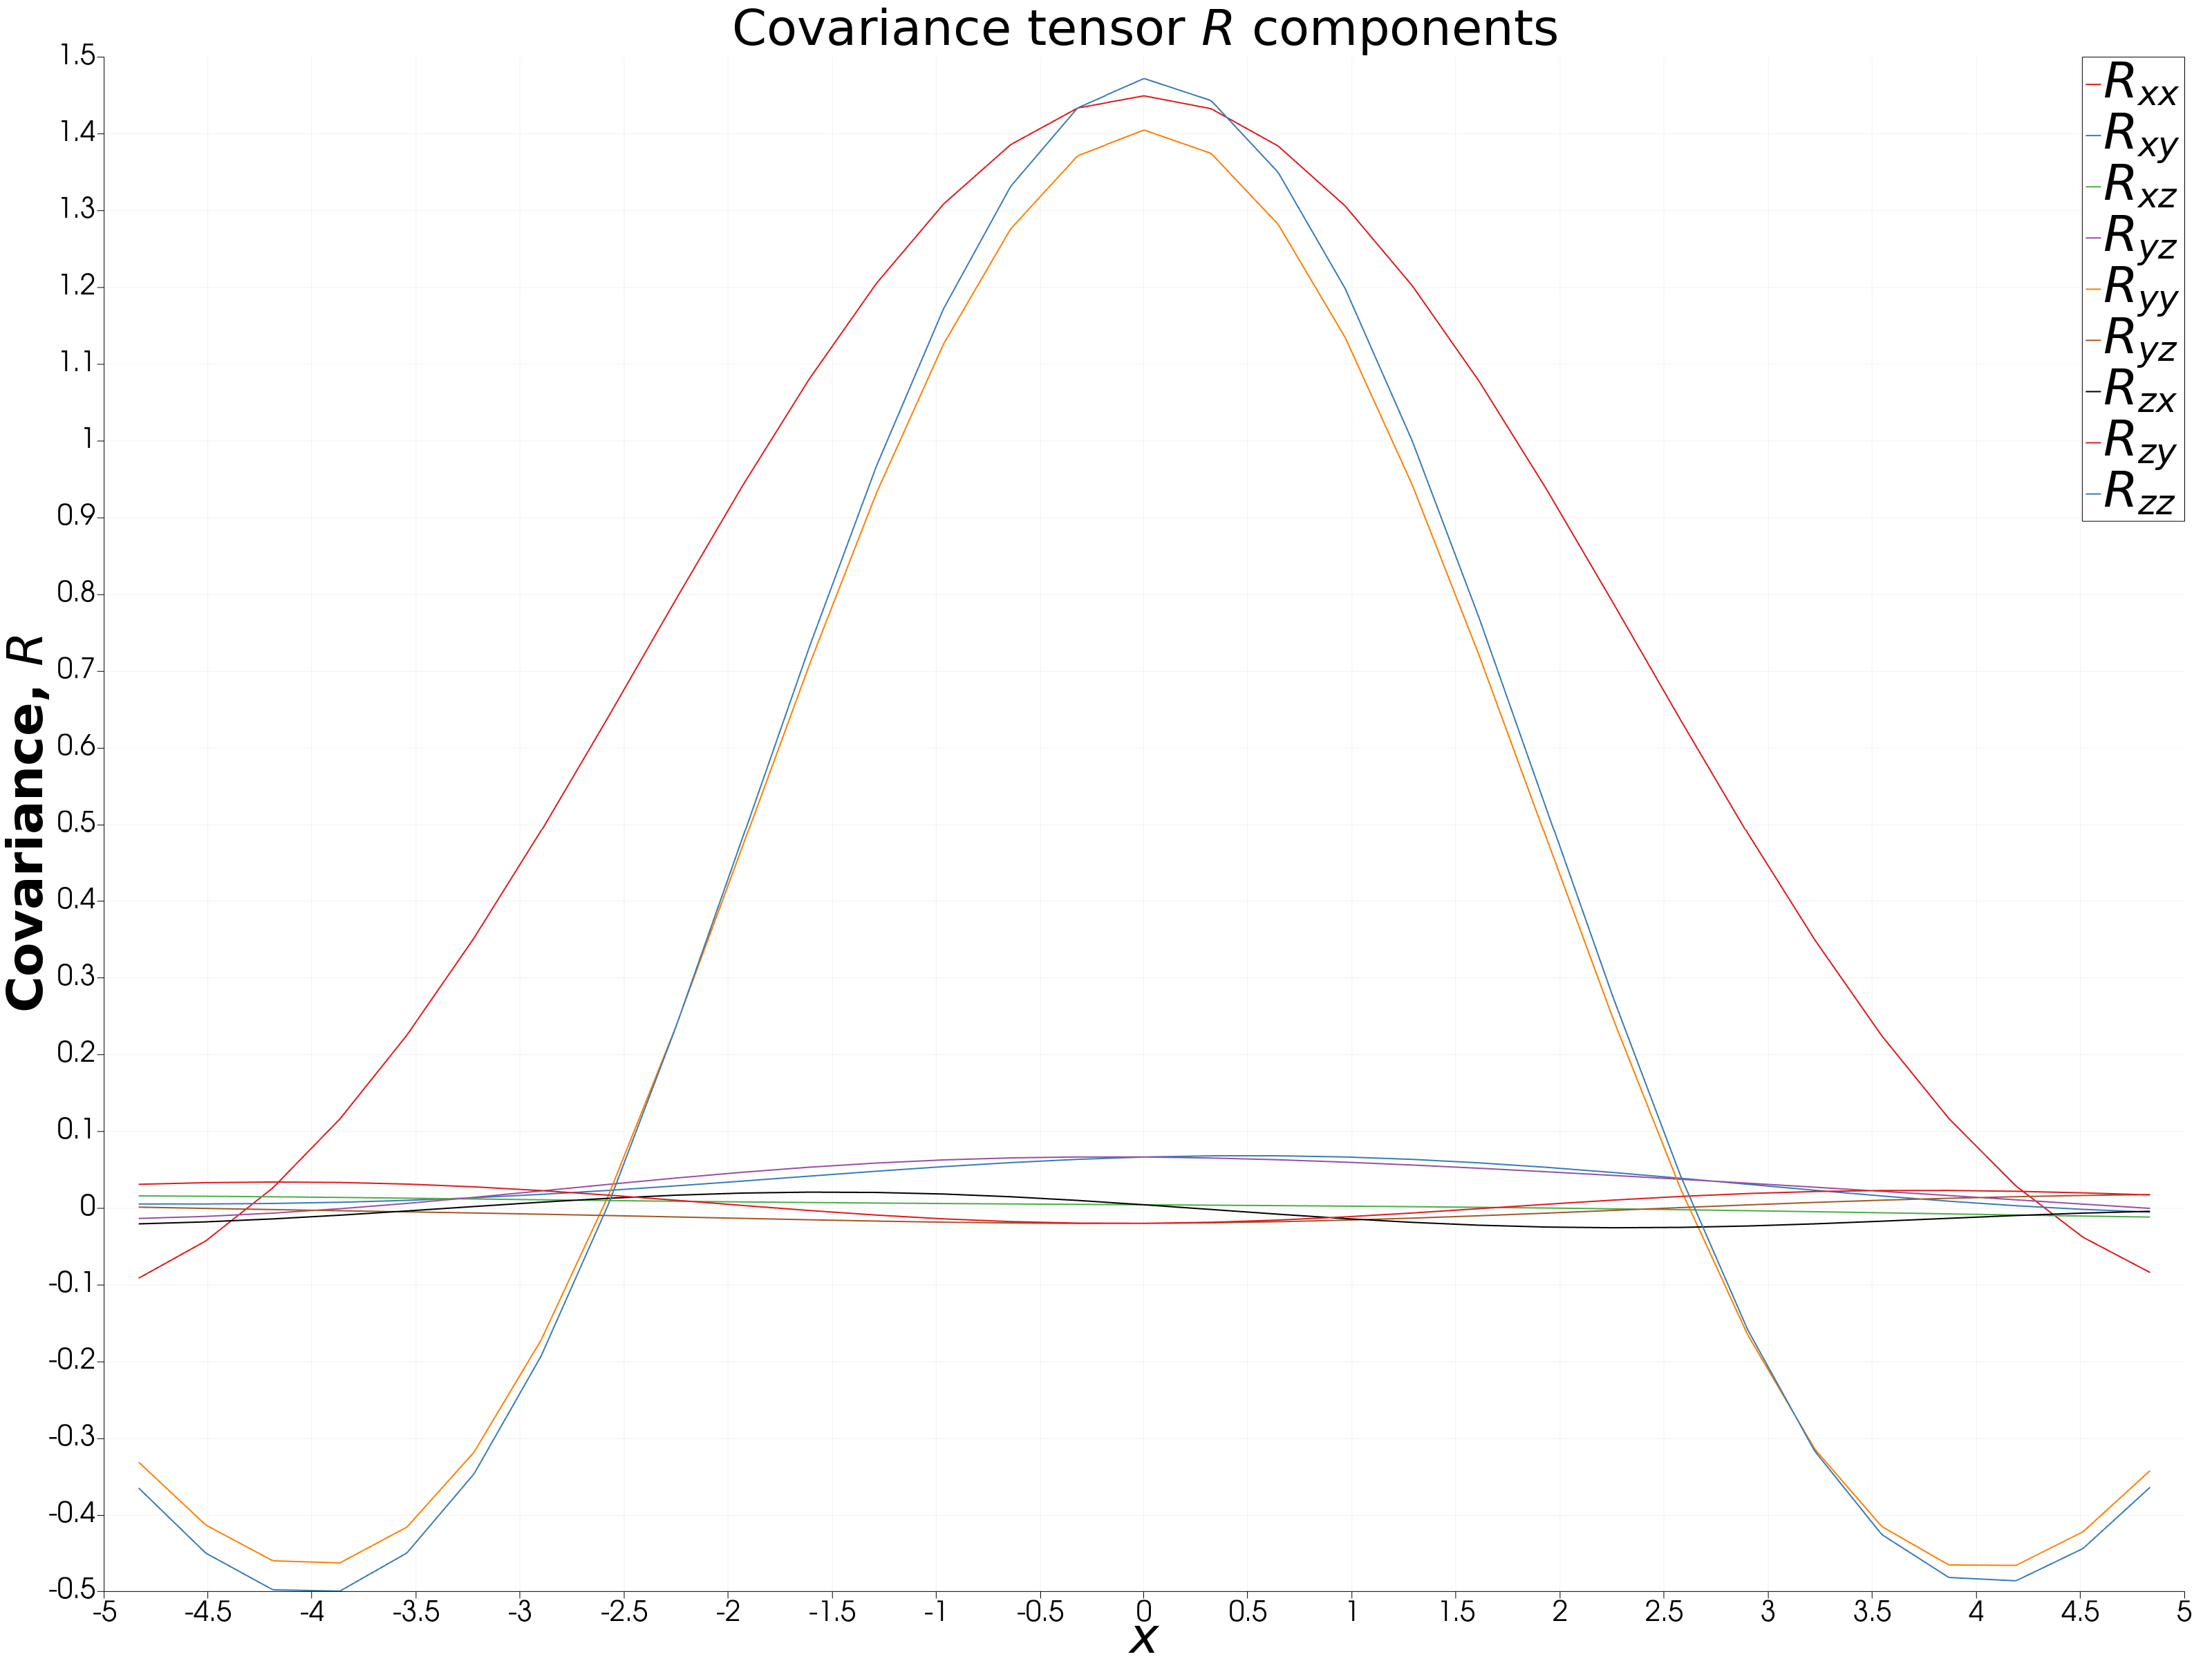
\includegraphics[width=0.45\linewidth]{images/spectral/spectral_n32_l10_f1000_k0pi3/covariance_function_x.png}} \\

    }
    \center{

        \subcaptionbox[List-of-Figures entry]{$y$\label{img:spectral_covariance_y}} 
        {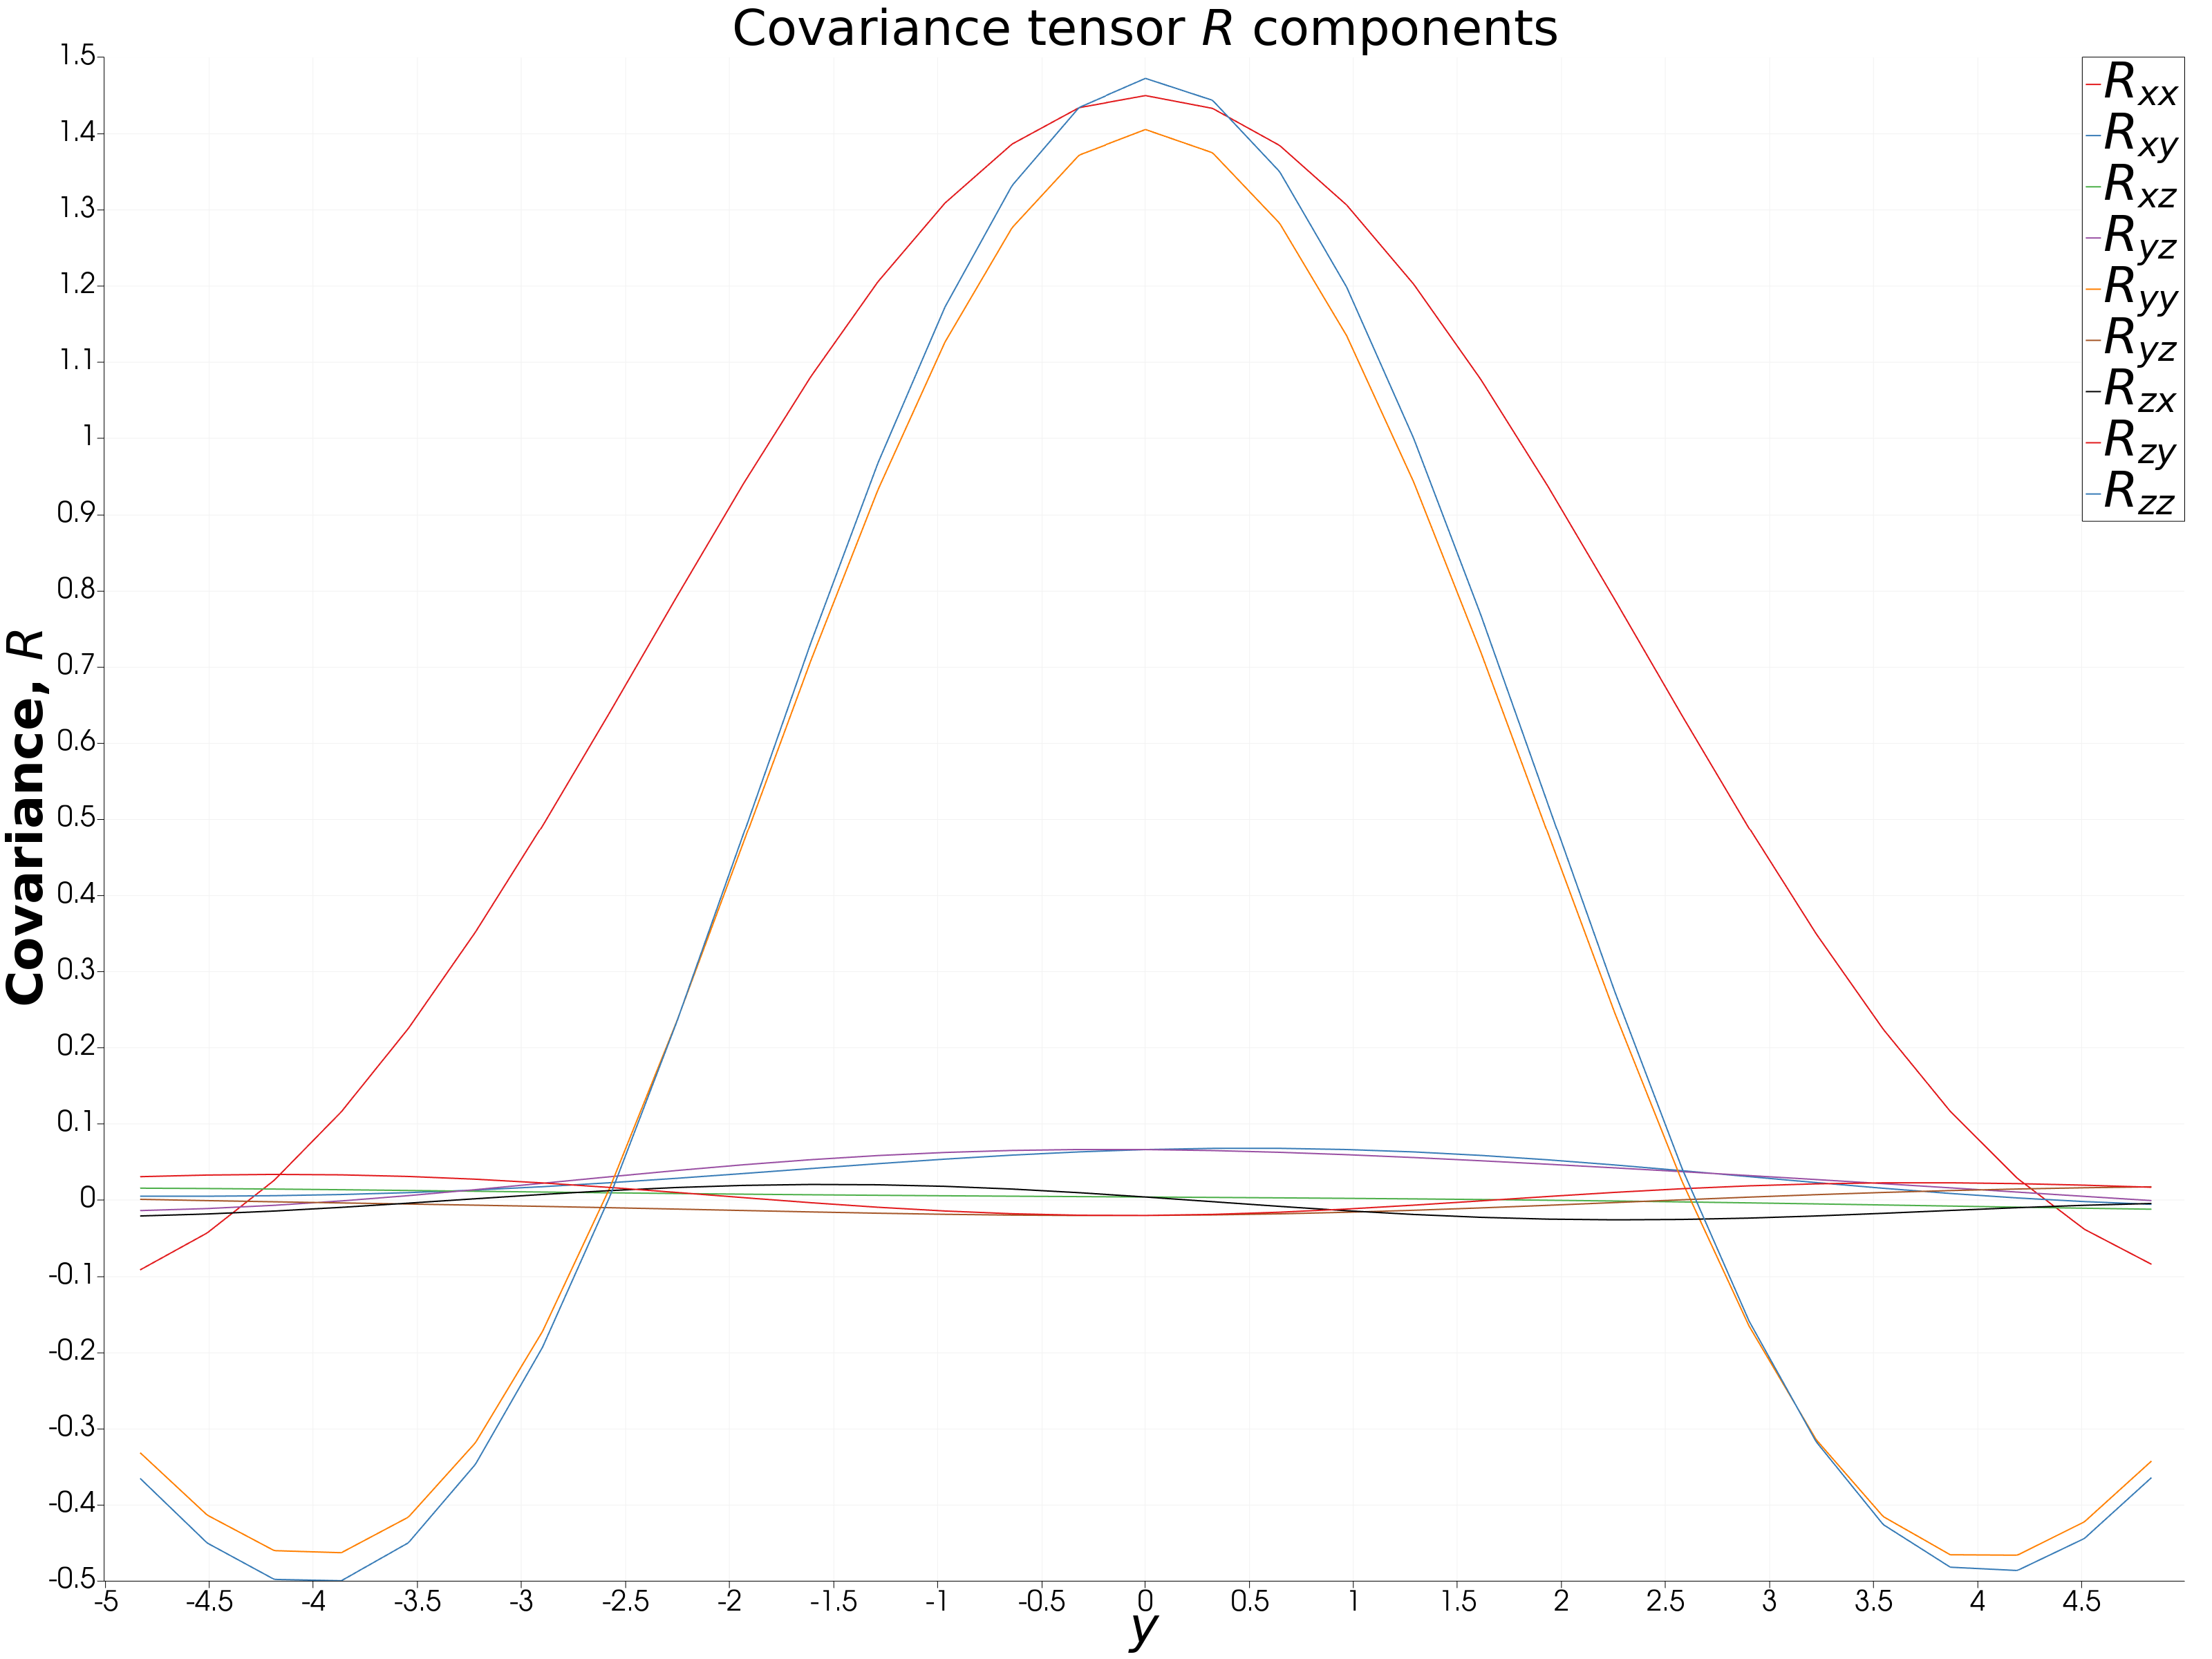
\includegraphics[width=0.45\linewidth]{images/spectral/spectral_n32_l10_f1000_k0pi3/covariance_function_y.png}}%
        \hfill
        \subcaptionbox{$z$\label{img:spectral_covariance_z}} 
        {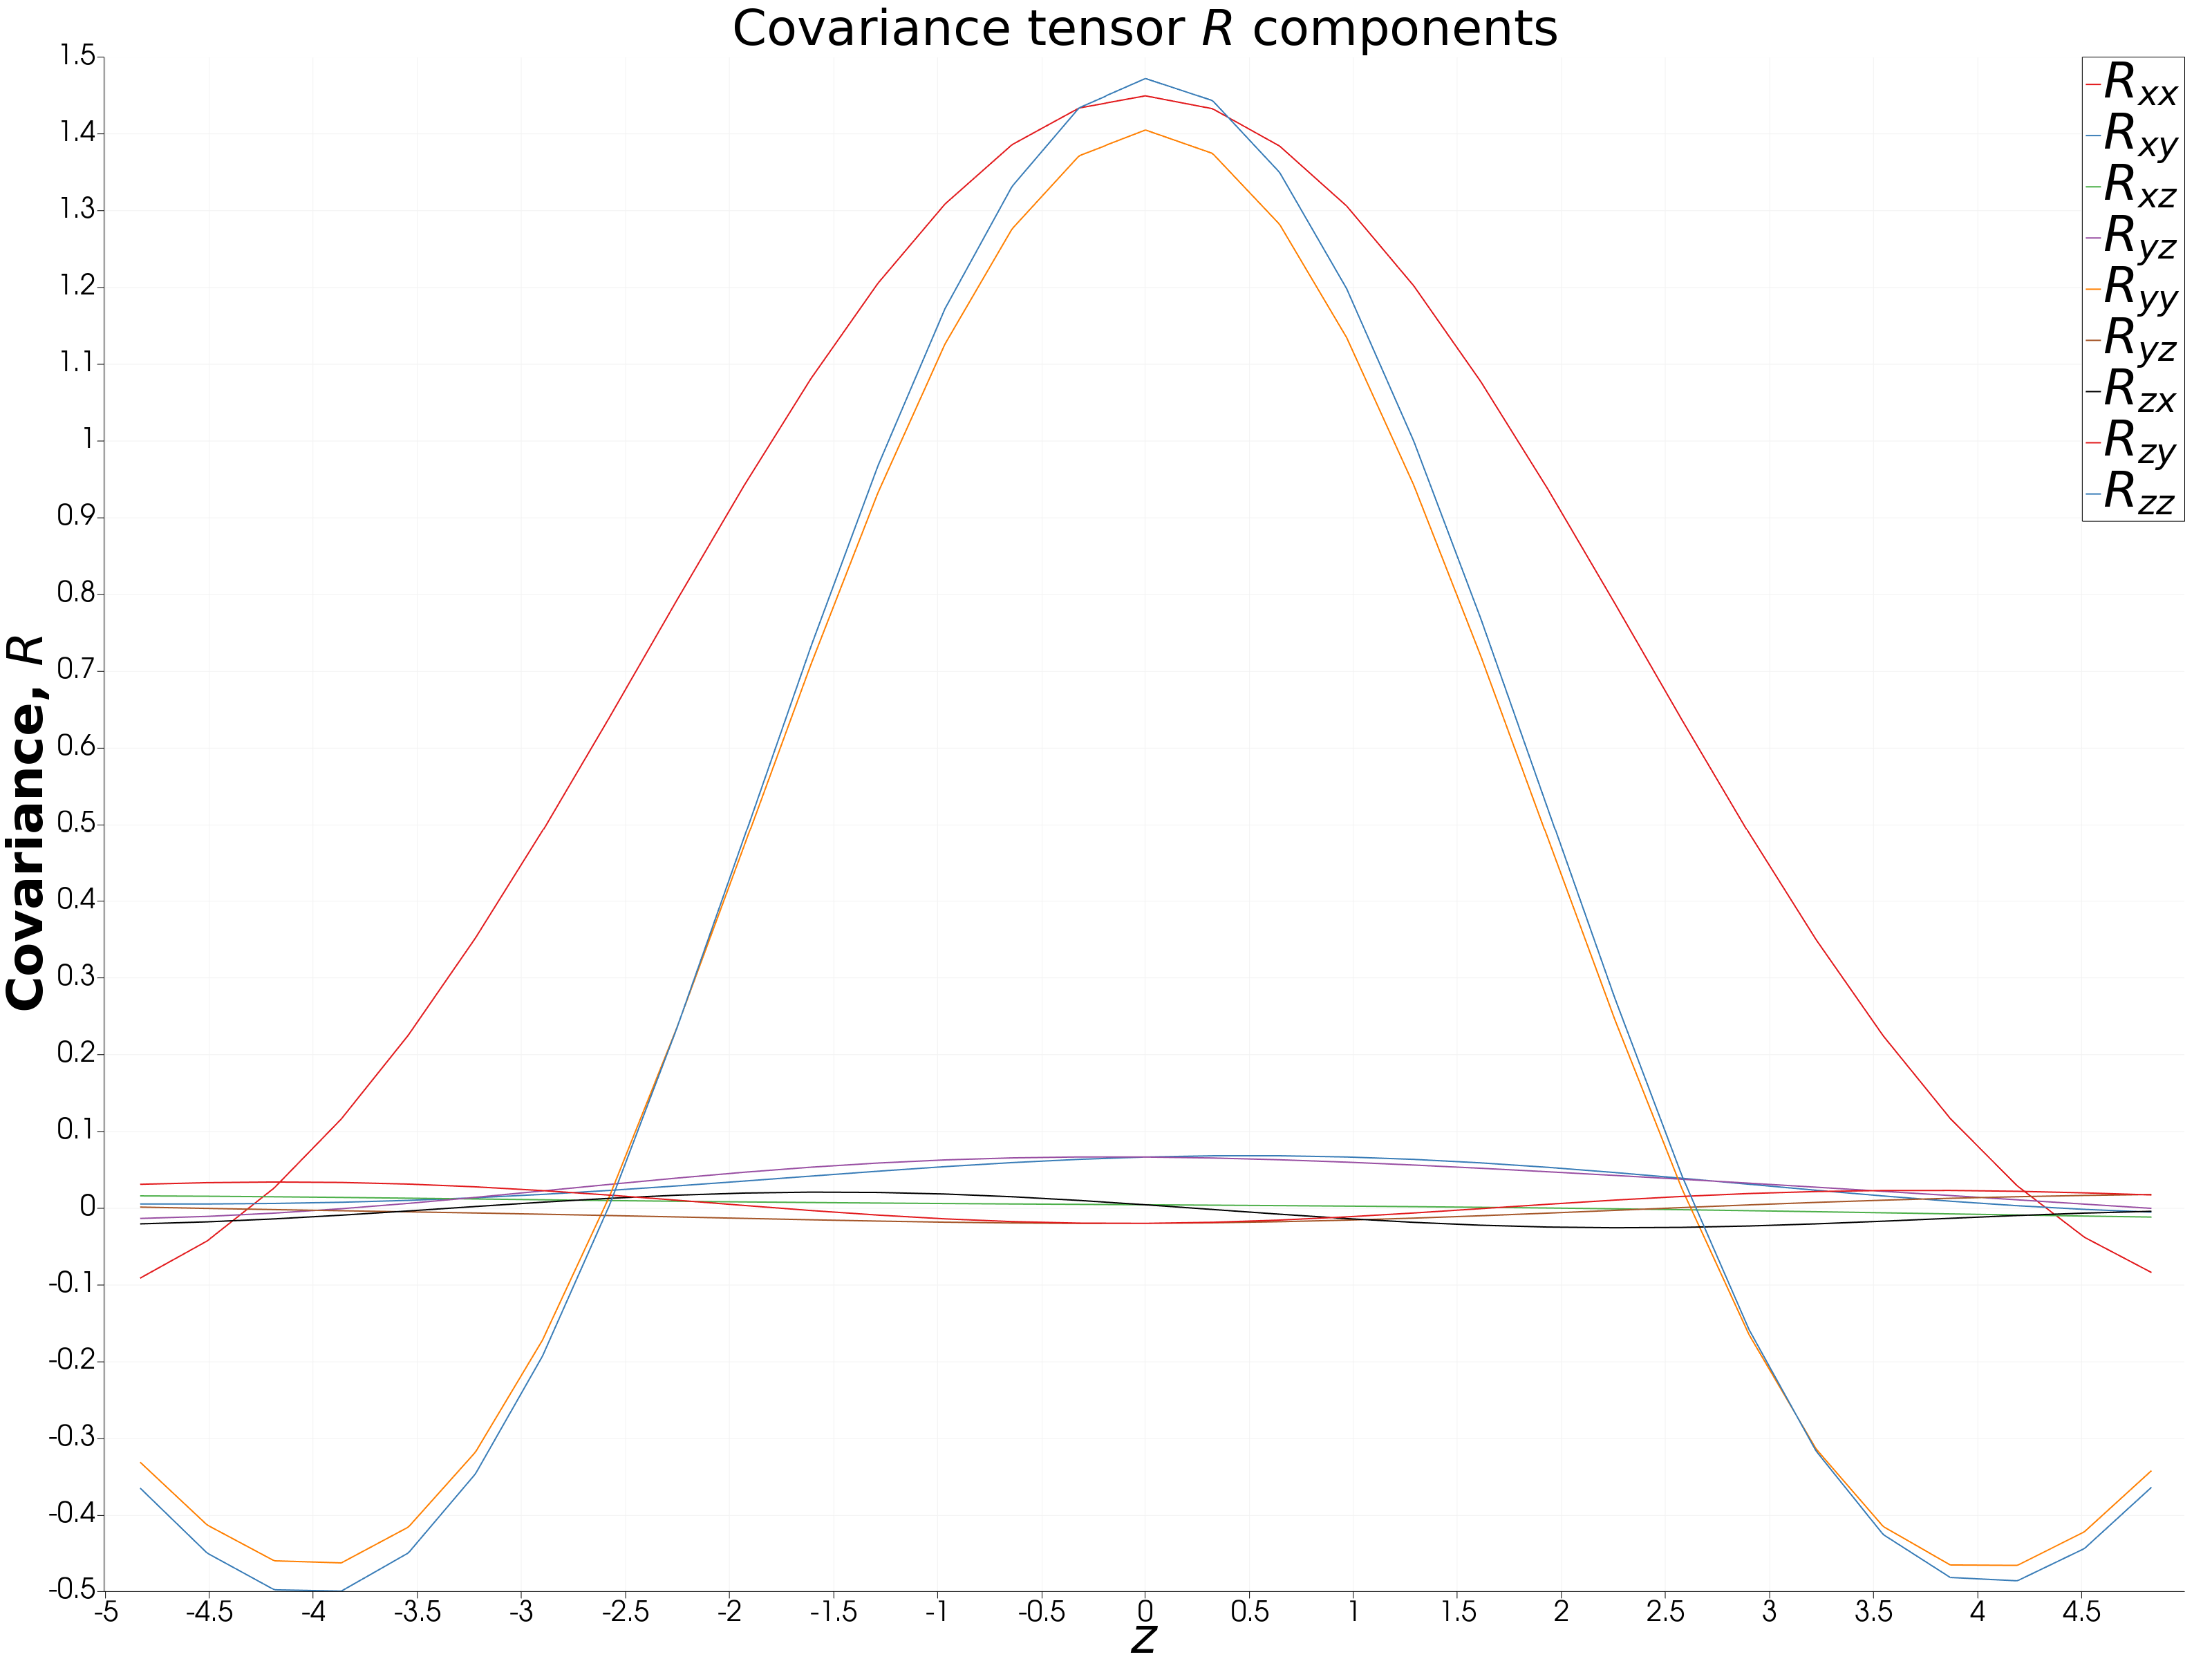
\includegraphics[width=0.45\linewidth]{images/spectral/spectral_n32_l10_f1000_k0pi3/covariance_function_z.png}}

    }
    
    \onehalfspacing{Поле на картинке б представлено с линиями тока, расчитанными вдоль оси $y$}
    \caption{Поле флуктуаций сгенерированных трёхмерным стохастическим методом, цветом обозначена амплитуда флуктуаций}
    \label{img:velocity_fluctuation_field_for_spectral_2}  
\end{figure}

По аналогии с методом Хуанга, мы можем генерировать поле флуктуаций как суперпозицию полей построенных для различных волновых чисел, а соответственно и для различных значений энергии. В этом случае $\vec u = \sum_{k_{i}} \vec u_i$, где $\vec u_i$ -- флуктуация, сгенерированная для определённого волнового числа $k_i$. Как и ранее, остается сложностью оценить наперед среднеквадратичное отклонение для проведения нормировки высоты спектральных линий для аппроксимации целевого спектра. Но мы можем сделать следующее, энергетический спектр турбулентности связан с кинетической энергии турбулентности $\kappa = \int_{0}^{\infty} E(k) dk$, отсюда мы можем взять, что $\kappa(k_m) = E(k_m) \Delta k$, и получаемую величину флуктуации скорости нормировать на значение $\sqrt{E(k_m) \Delta k}$. 

Одним из других подходов состоит в нормировке не результирующего значения флуктуации, а в нормировке амплитуд мод Фурье. В отличие от нормировки результирующего вектора флуктуаций, в данном подходе на выходе также получаются различные амплитуды флуктуаций с сохранением зависимости от амплитуды спектра. Для ускорения процесса генерации можно использовать разложение лишь по одной тригонометрической функции, например лишь по функции косинуса. В итоге можно использовать разложение представленное в виде:

\begin{equation}
    \label{eq:part3_3}
    \vec v(\vec r, t) = \alpha \sum_{n = 1}^{N} \vec p_n \cos( \vec k_n \cdot \vec r + \omega_n \cdot t + \psi)  
\end{equation}

\noindent 
здесь, $\vec p_n$ -- амплитуды мод Фурье, генерируемые изначально на единичной сфере так, чтобы $\vec p_n \cdot \vec k_n = 0$, для сохранения удовлетворению уравнению неразрывности, с последующим привидением к длине равной $\sqrt{E(k_n)\Delta k}$, $\psi_n$ - случайная фаза, добавленная для компенсации исключения нечетных мод, генерируемая например из равномерного распределения в пределах $-\pi$ до $\pi$, $\alpha$ -- нормировочный коэффициент, который можно взять, например $\sqrt{\frac{2}{N}}$, как в методе Смирнова(\ref{sect2_2}), либо провести нормировки на кинетическую энергию по аналогии с методом Шура (\ref{sect2_4}): $\sqrt{\frac{1}{\sum_{n=1}^{N} E(k_n) \Delta k_n}}$. По построению амплитуд Фурье лучше всего использовать последнее определение для нормировочного коэффициента $\alpha = \sqrt{\frac{\beta}{\sum_{n=1}^{N} E(k_n) \Delta k_n}}$, после проведения тестовых расчётов мы получили что оптимальным значение для коэффициента $\beta \approx 2$. Связано это с тем, чтобы в формуле \eqref{eq:kriging_equation15} компенсировать коэффициент $\frac{1}{2}$. 

Для проведения статистического анализа предлагаемой модификации спектрального метода использовалось 5000 реализаций со следующими параметрами:
\begin{enumerate}
    \item Длина куба: $l = 10$, центр совпадает с началом координат;
    \item Число разбиений по каждой из сторон куба: $n = 51$;
    \item Число взятых мод Фурьe: $N = 1000$;
    \item Интервал волновых чисел: $(k_{min} = 0.01, k_{max} = 10$, число разбиений для дискретизации спектра совпадает с числом мод Фурье;
\end{enumerate}

Наименьшее волновое число для рассматриваемой сетке: $k_{min} = \frac{2 \pi}{l} \approx 0.6283$ -- максимальное волновое число: $k_{max} = \frac{\pi}{\frac{l}{n}} \approx 16.022$. Приведём сравнение спектра рассчитанного для приведённого выше числа сгенерированных реализаций с входным спектром.

\begin{figure}[ht] 
    \center
    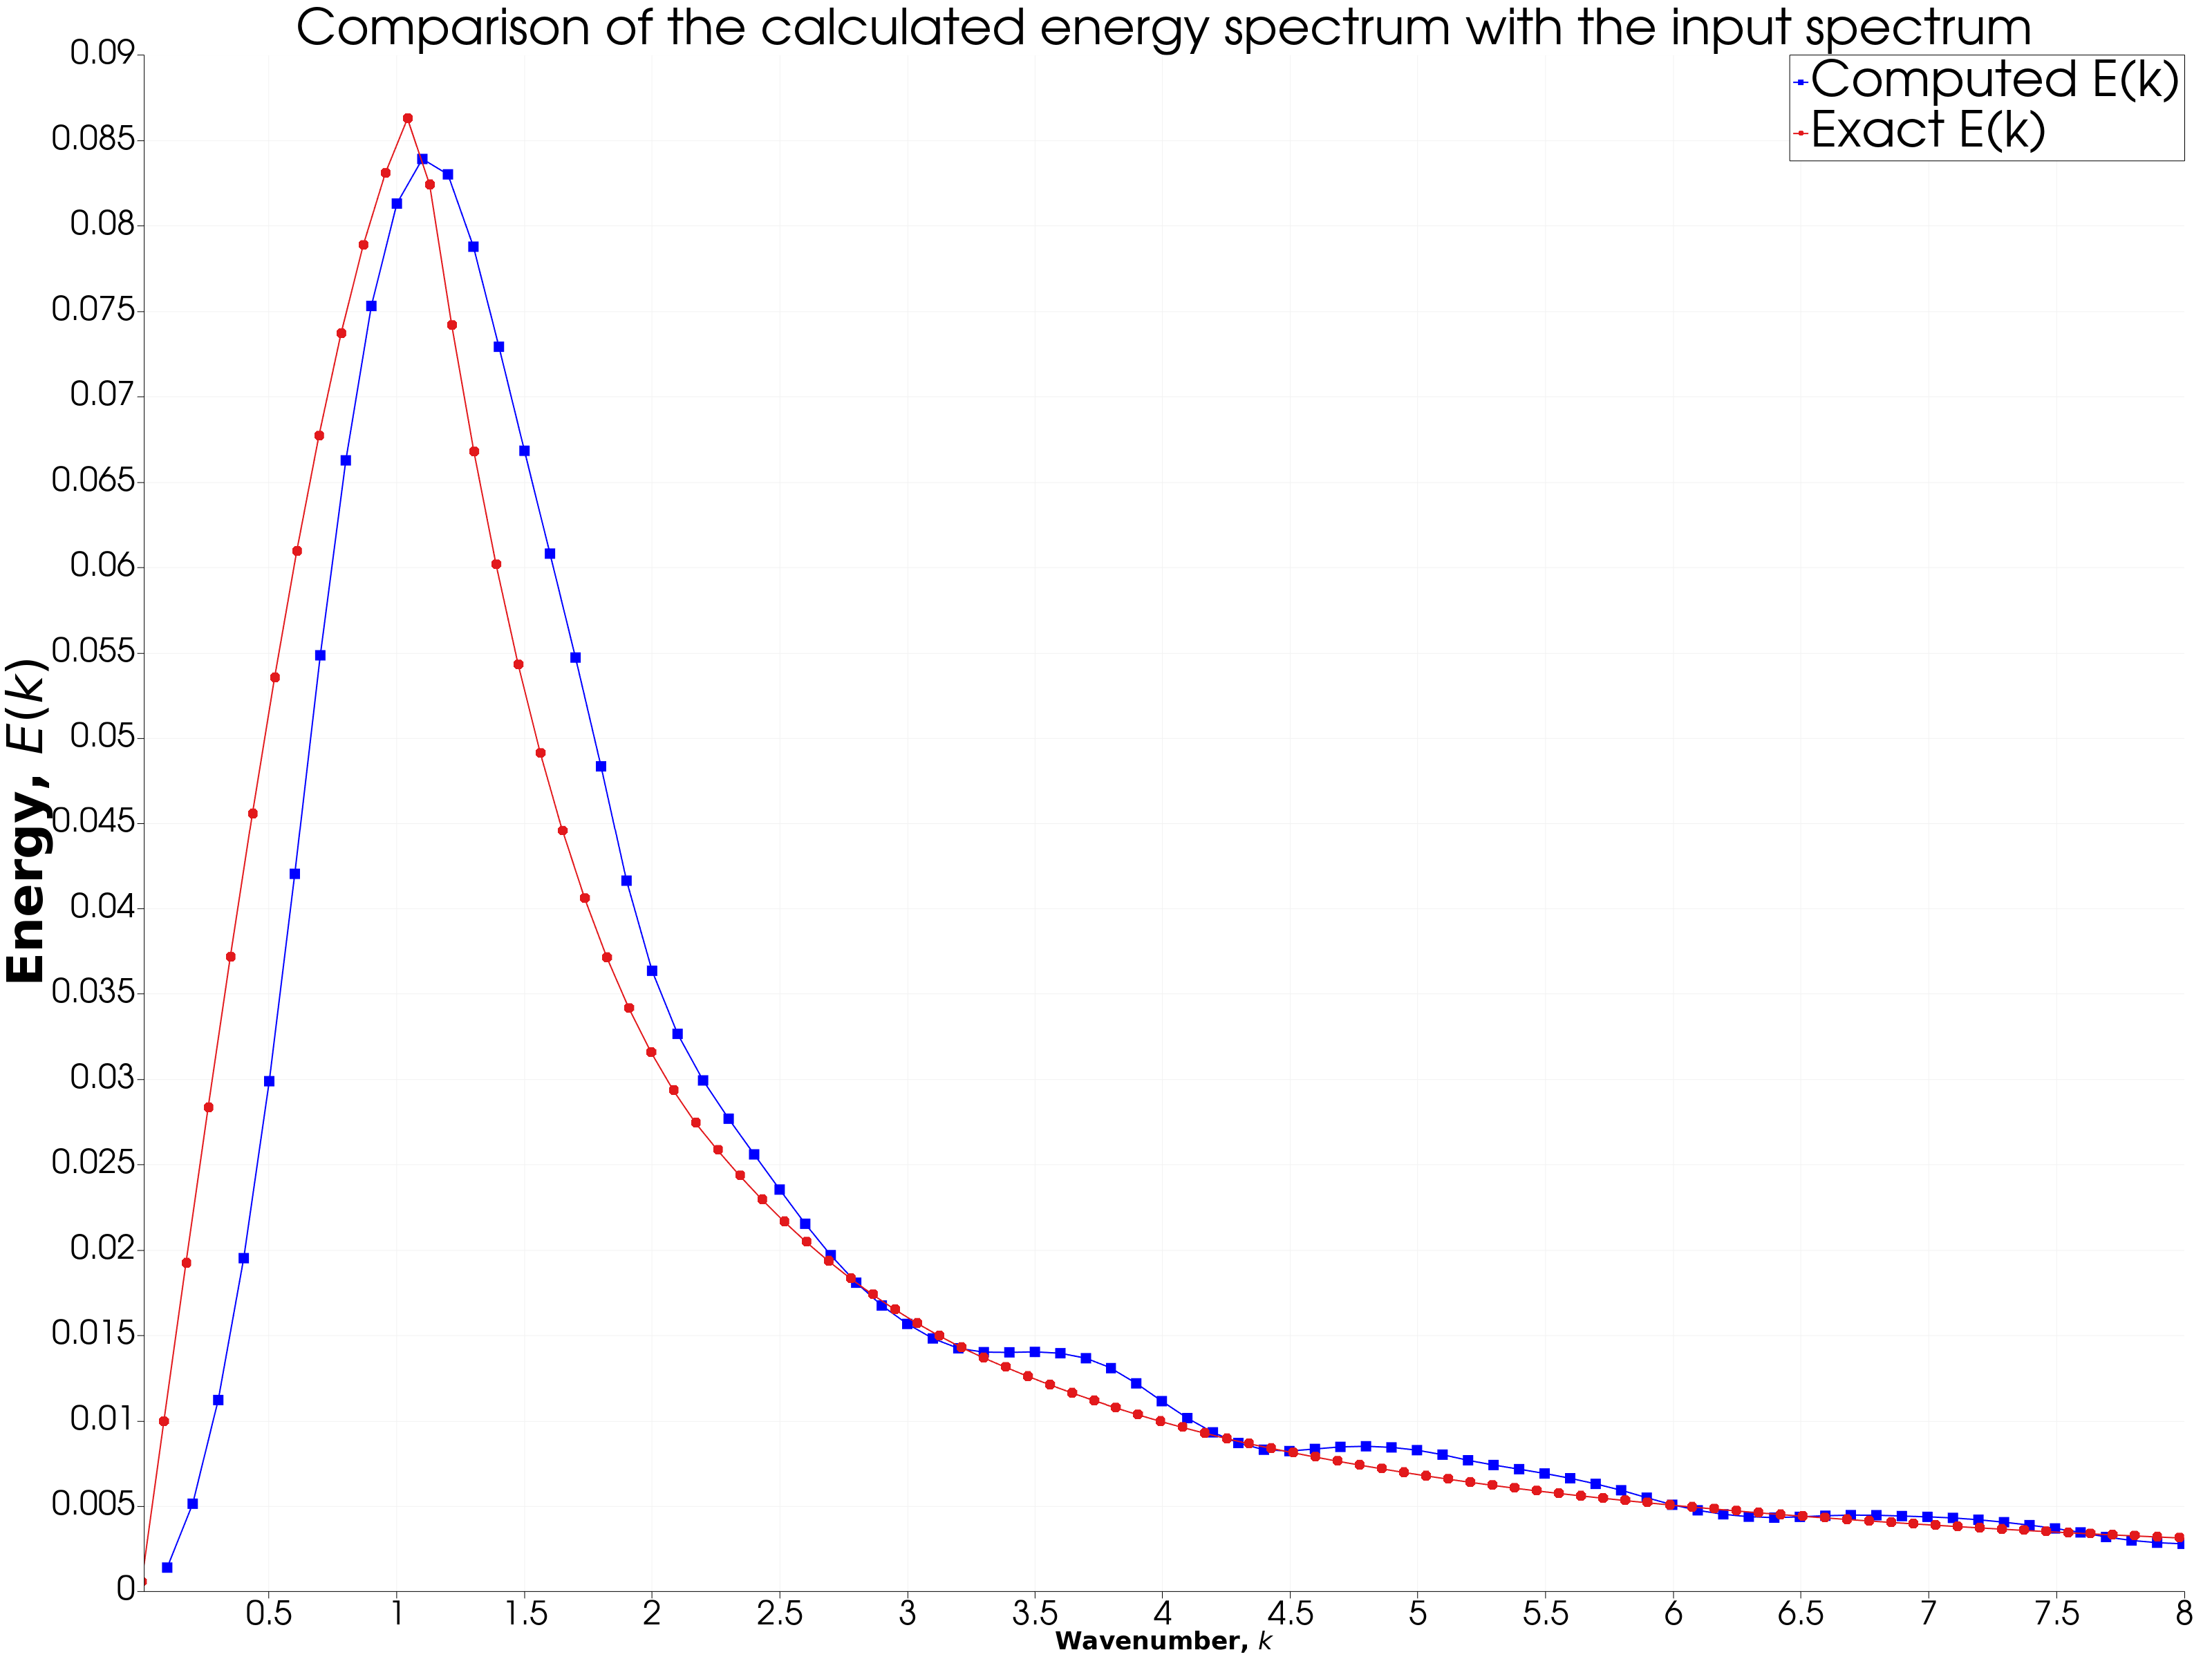
\includegraphics [width=0.8\linewidth] {images/spectral/spectra_l10_k10_f1000_n51.png}
    \caption{Сравнение энергетического спектра для предлагаемой модификации спектрального метода с задаваемым.} 
    \label{img:spectral_desam_spectra_comarison}  
\end{figure}

\begin{figure}[ht] 
    \center
    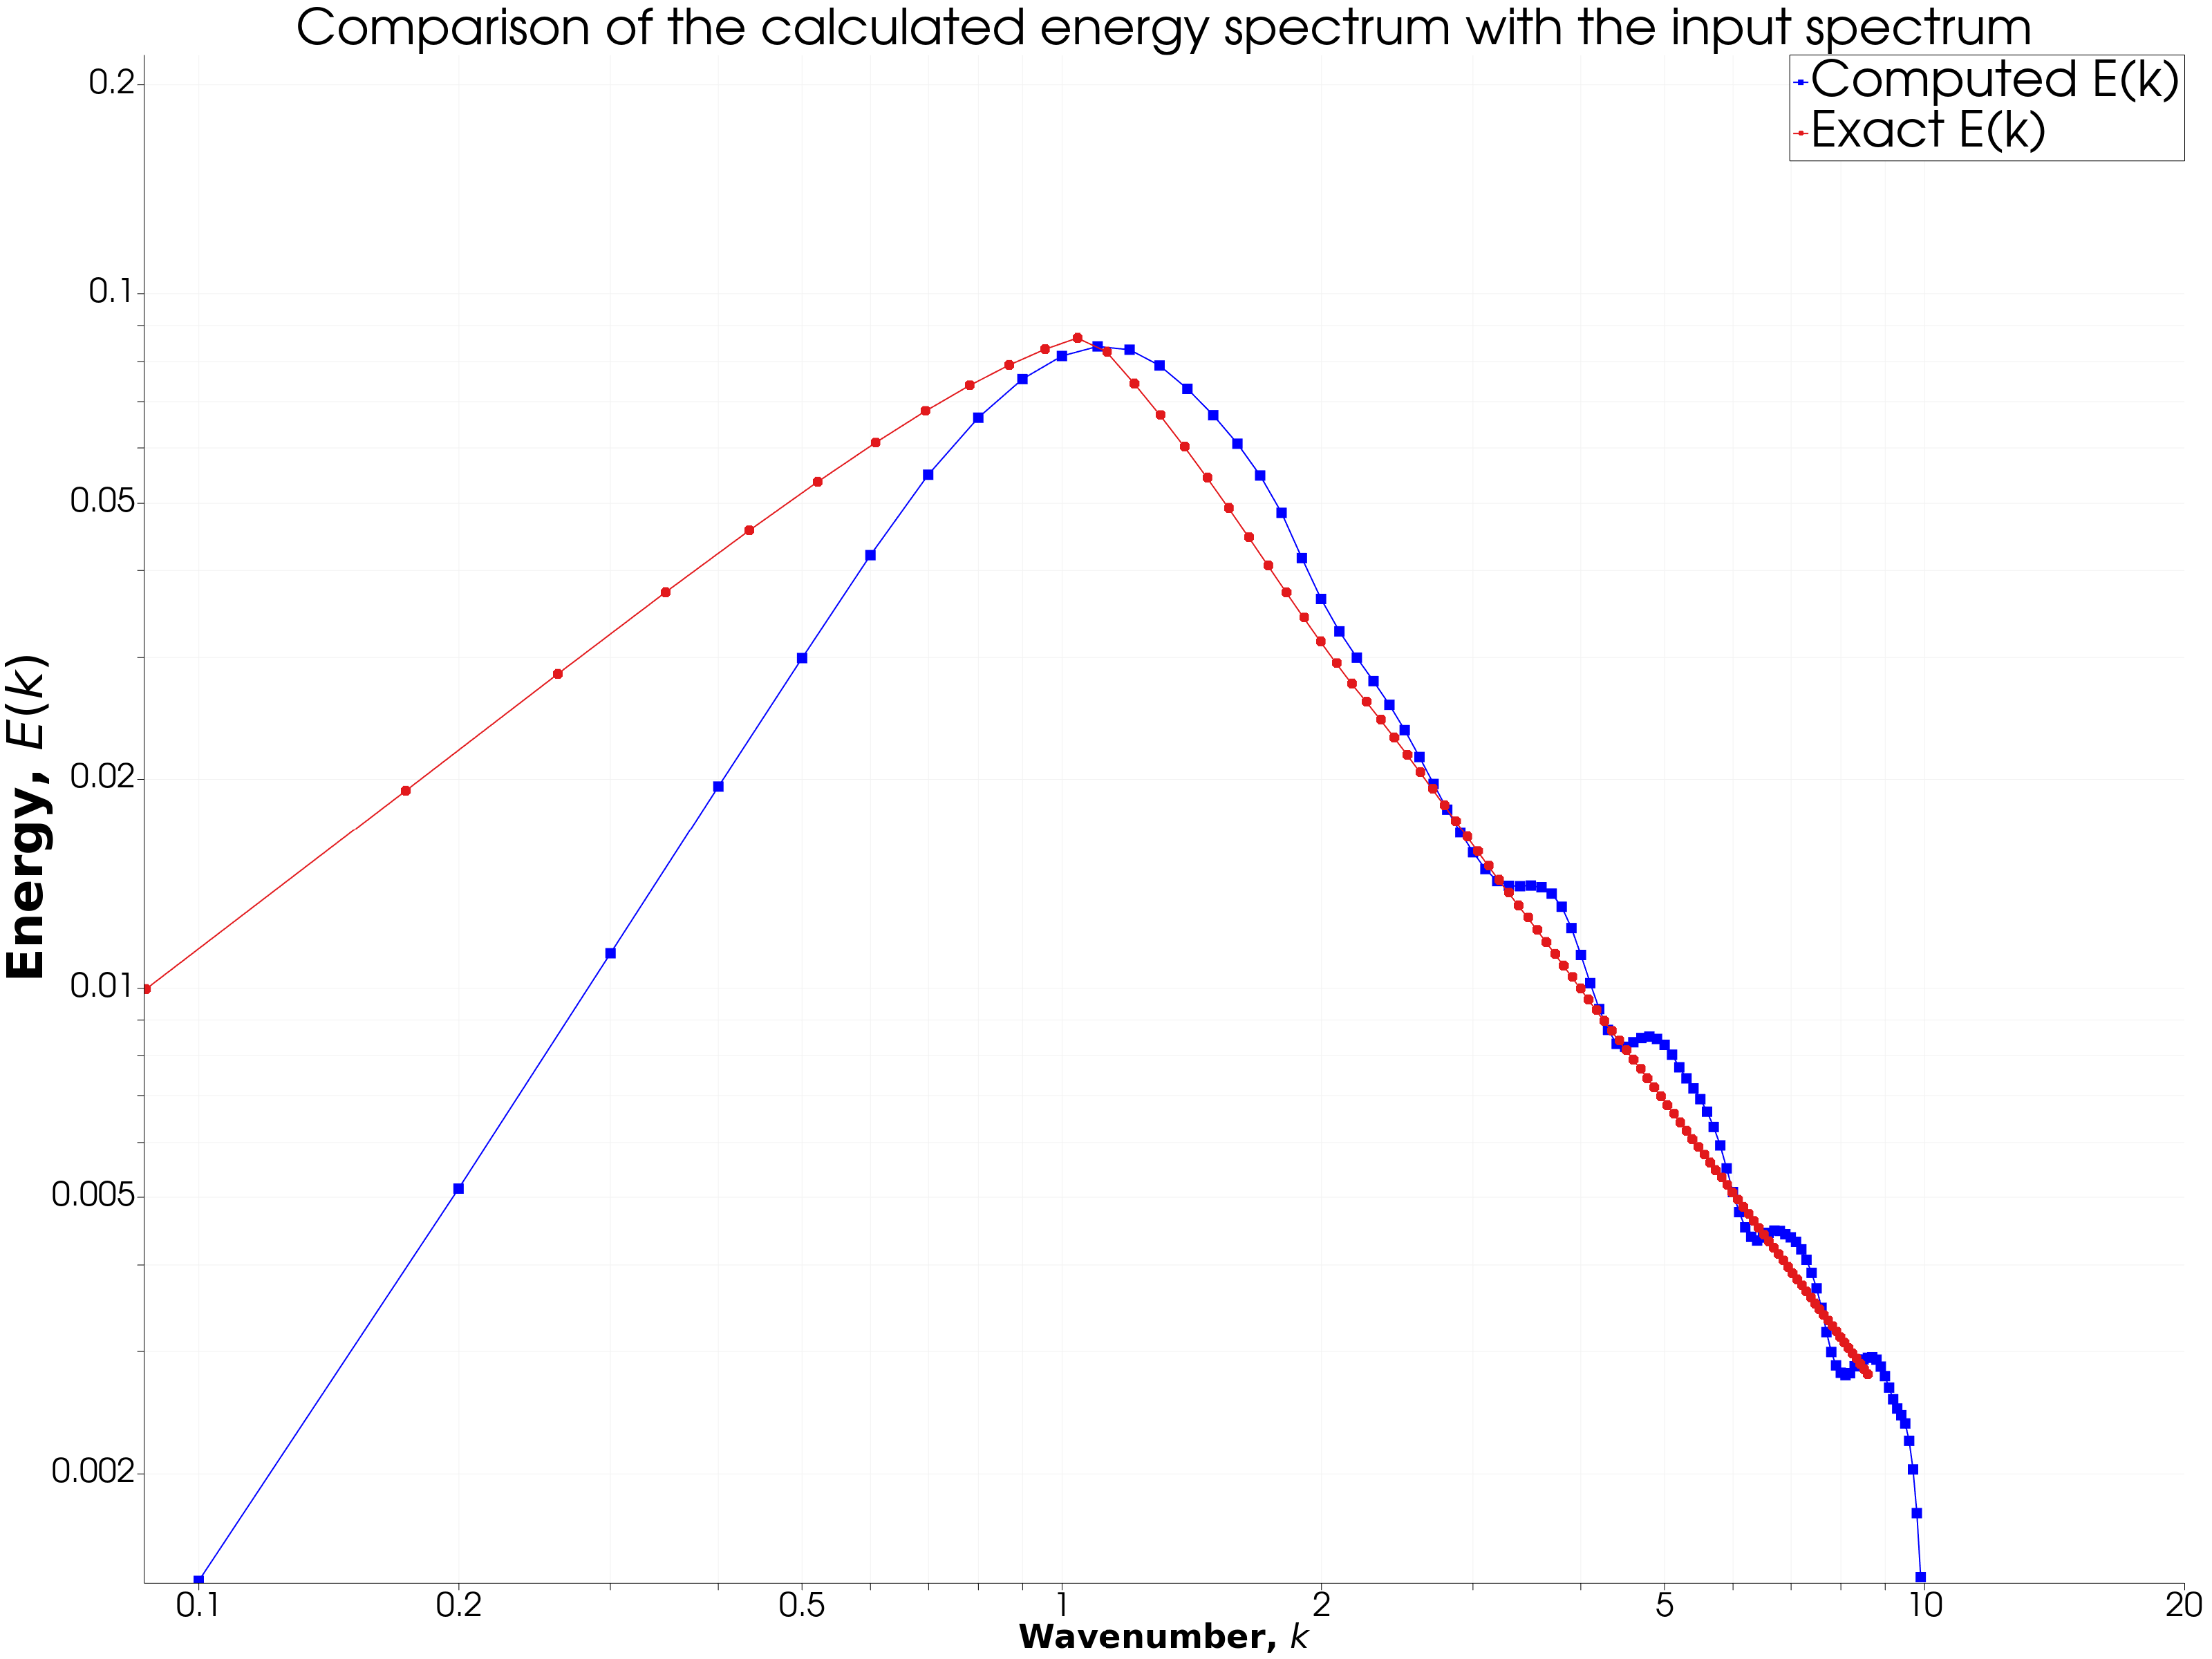
\includegraphics [width=0.8\linewidth] {images/spectral/spectra_l10_k10_f1000_n51_loglog.png}
    \caption{Сравнение энергетического спектра для предлагаемой модификации спектрального метода с задаваемым в логарифмических координатах} 
    \label{img:spectral_desam_spectra_comparison}  
\end{figure}

Во первых заметим большую разницу для малых значений волнового числа, связанное с тем что минимальное волновое число меньше чем волновое число для рассматриваемой сетке, в свою очередь в диапазоне начиная с минимального для сетки волнового числа наблюдается хорошее совпадение с целевым спектром, особенно в инерционном интервале, с хорошо известным законом $-\dfrac{5}{3}$.
  
\begin{figure}[ht] 
    \center
    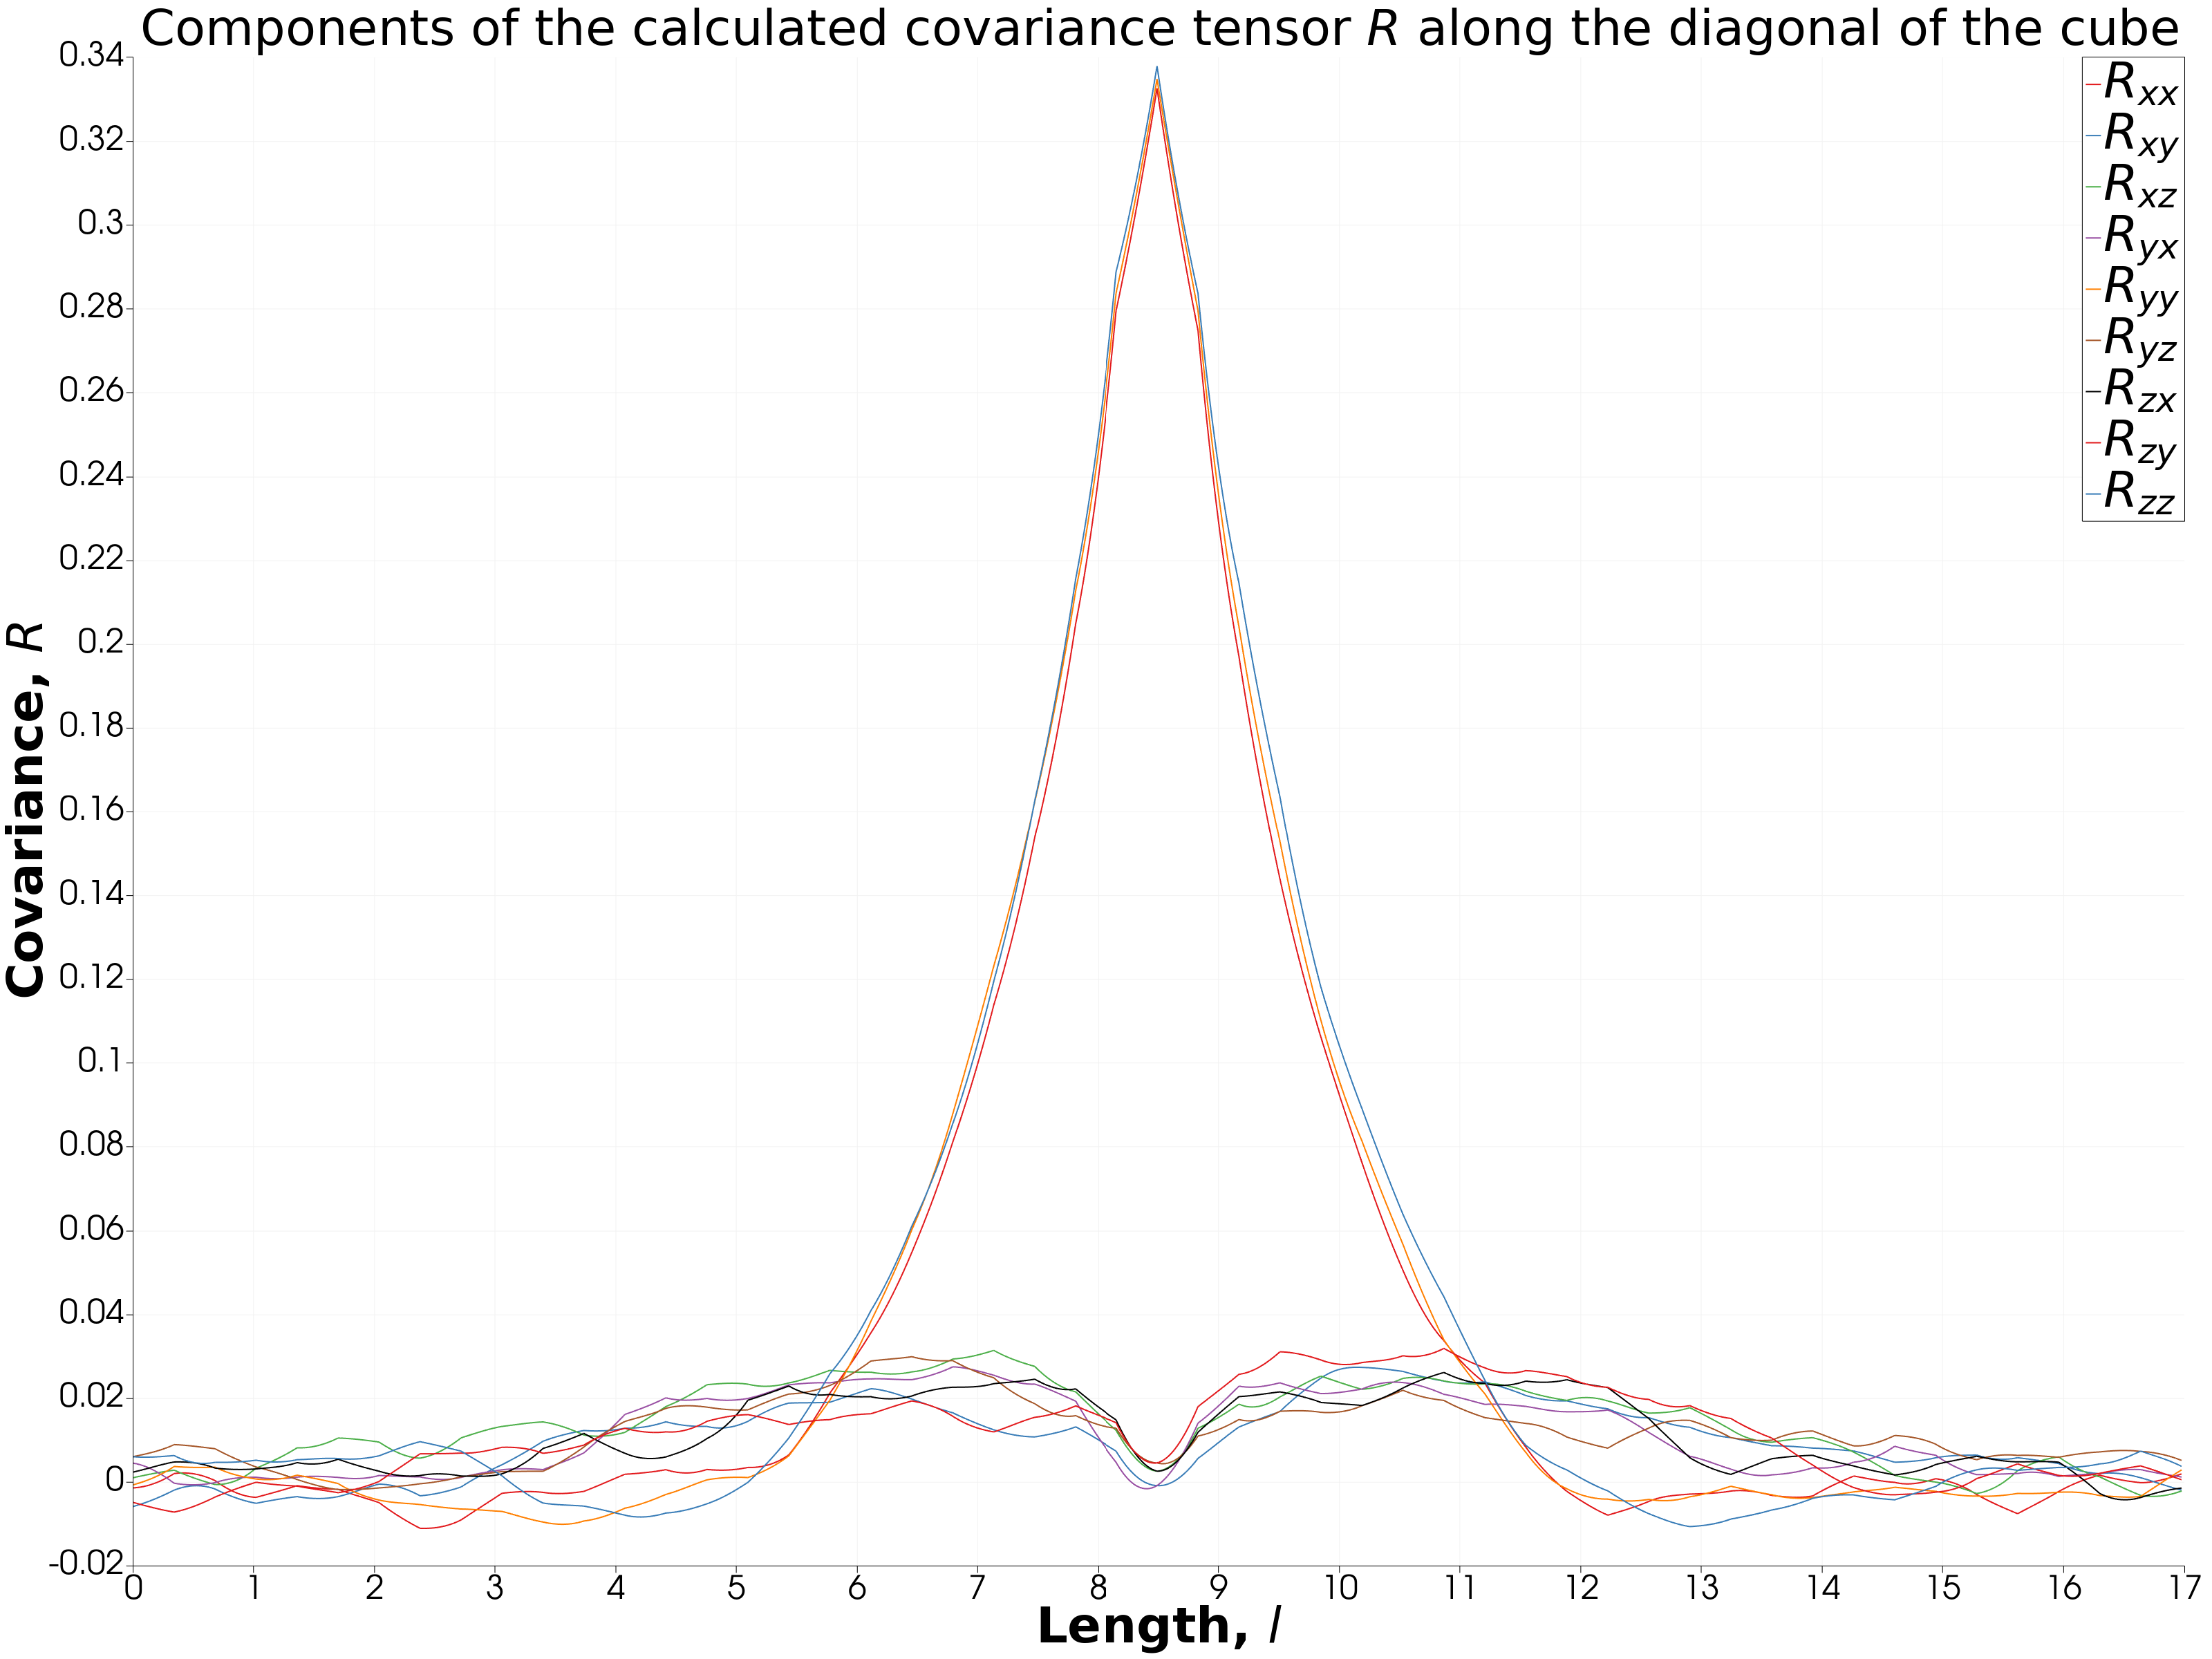
\includegraphics [width=0.8\linewidth] {images/spectral/covariance_function_tensor.png}
    \caption{Компоненты тензора ковариаций вдоль диагонали вычислительной области} 
    \label{img:spectral_desam_covariance_comarison}  
\end{figure}

Сразу можно заметить, что по сравнению с генерацией на одной частоте, а именно методом Крайшнана, амплитуда ковариаций уменьшая быстрее с ростом расстояния от центра расчёта ковариации. Также уменьшилось расстояние на котором сохраняется пространственная ковариация двух величин, как было показано ранее, функция ковариации при генерации одной амплитуды сохраняет ковариацию на больших расстояниях, и имеет форму модулированной волны, в рассматриваемом сейчас случае, при достижении амплитуды ковариации при дальнейшем увеличении расстояния коррелированность величин остается близи 0.

Приведём несколько сгенерированных полей флуктуаций с использованием предложенного метода. На рисунках ниже представлено по 3 плоскости с отображением направлений флуктуаций, для того чтобы показаться изменение векторов не только в плоскости $yz$ по нормали к оси $x$, центр поддомена совпадает с центром расчётной области.


\begin{figure}[ht] 
    \center
    \includegraphics [width=0.8\linewidth] {images/spectral/field_on_x_normal_yz_plane.png}
    \caption{Сгенерированное поле флуктуаций модифицированным методом, длины векторов пропорциональны длине векторов флуктуаций} 
    \label{img:spectral_result_field_no_angle}  
\end{figure}

\begin{figure}[ht] 
    \center
    \includegraphics [width=0.8\linewidth] {images/spectral/field_on_angle.png}
    \caption{Сгенерированное поле флуктуаций модифицированным методом, длины векторов пропорциональны длине векторов флуктуаций} 
    \label{img:spectral_result_field_on_angle}  
\end{figure}

На представленных рисунках хорошо видно вихревое движение во всех направлениях. За счёт пропорциональности длины векторов мы можем явно качественно разделить течение на зоны. 

Для сравнения методов по производительности использовалась сетка размерностью $n = 31$ и размером $l=10$. Для спектрального метода использовалось 1000 мод фурье с покрытием всего интервала волновых чисел, с такими параметрами достигается максимальная производительность не в угоду точности. Замер среднего времени генерации проводился на 1000 генераций. Полное время, потребовавшееся для генерации 1000 реализаций составило в среднем ~44 секунды, среднее время для генерации одной реализации поля скорости $\frac{44}{1000} \approx 0.044$, пренебрегая временем на операции записи результатов в файл.

По построению флуктуаций скоростей, спектральный метод также должен на выходе давать поле скоростей удовлетворяющее уравнению неразрывности для несжимаемой жидкости $\vec \nabla \cdot \vec v = 0$. Вычислим на сетке также величину $\vec \nabla \cdot \vec v$ характеризующую отклонение от условия неразрывности. 

\begin{figure}[ht] 
    \center
    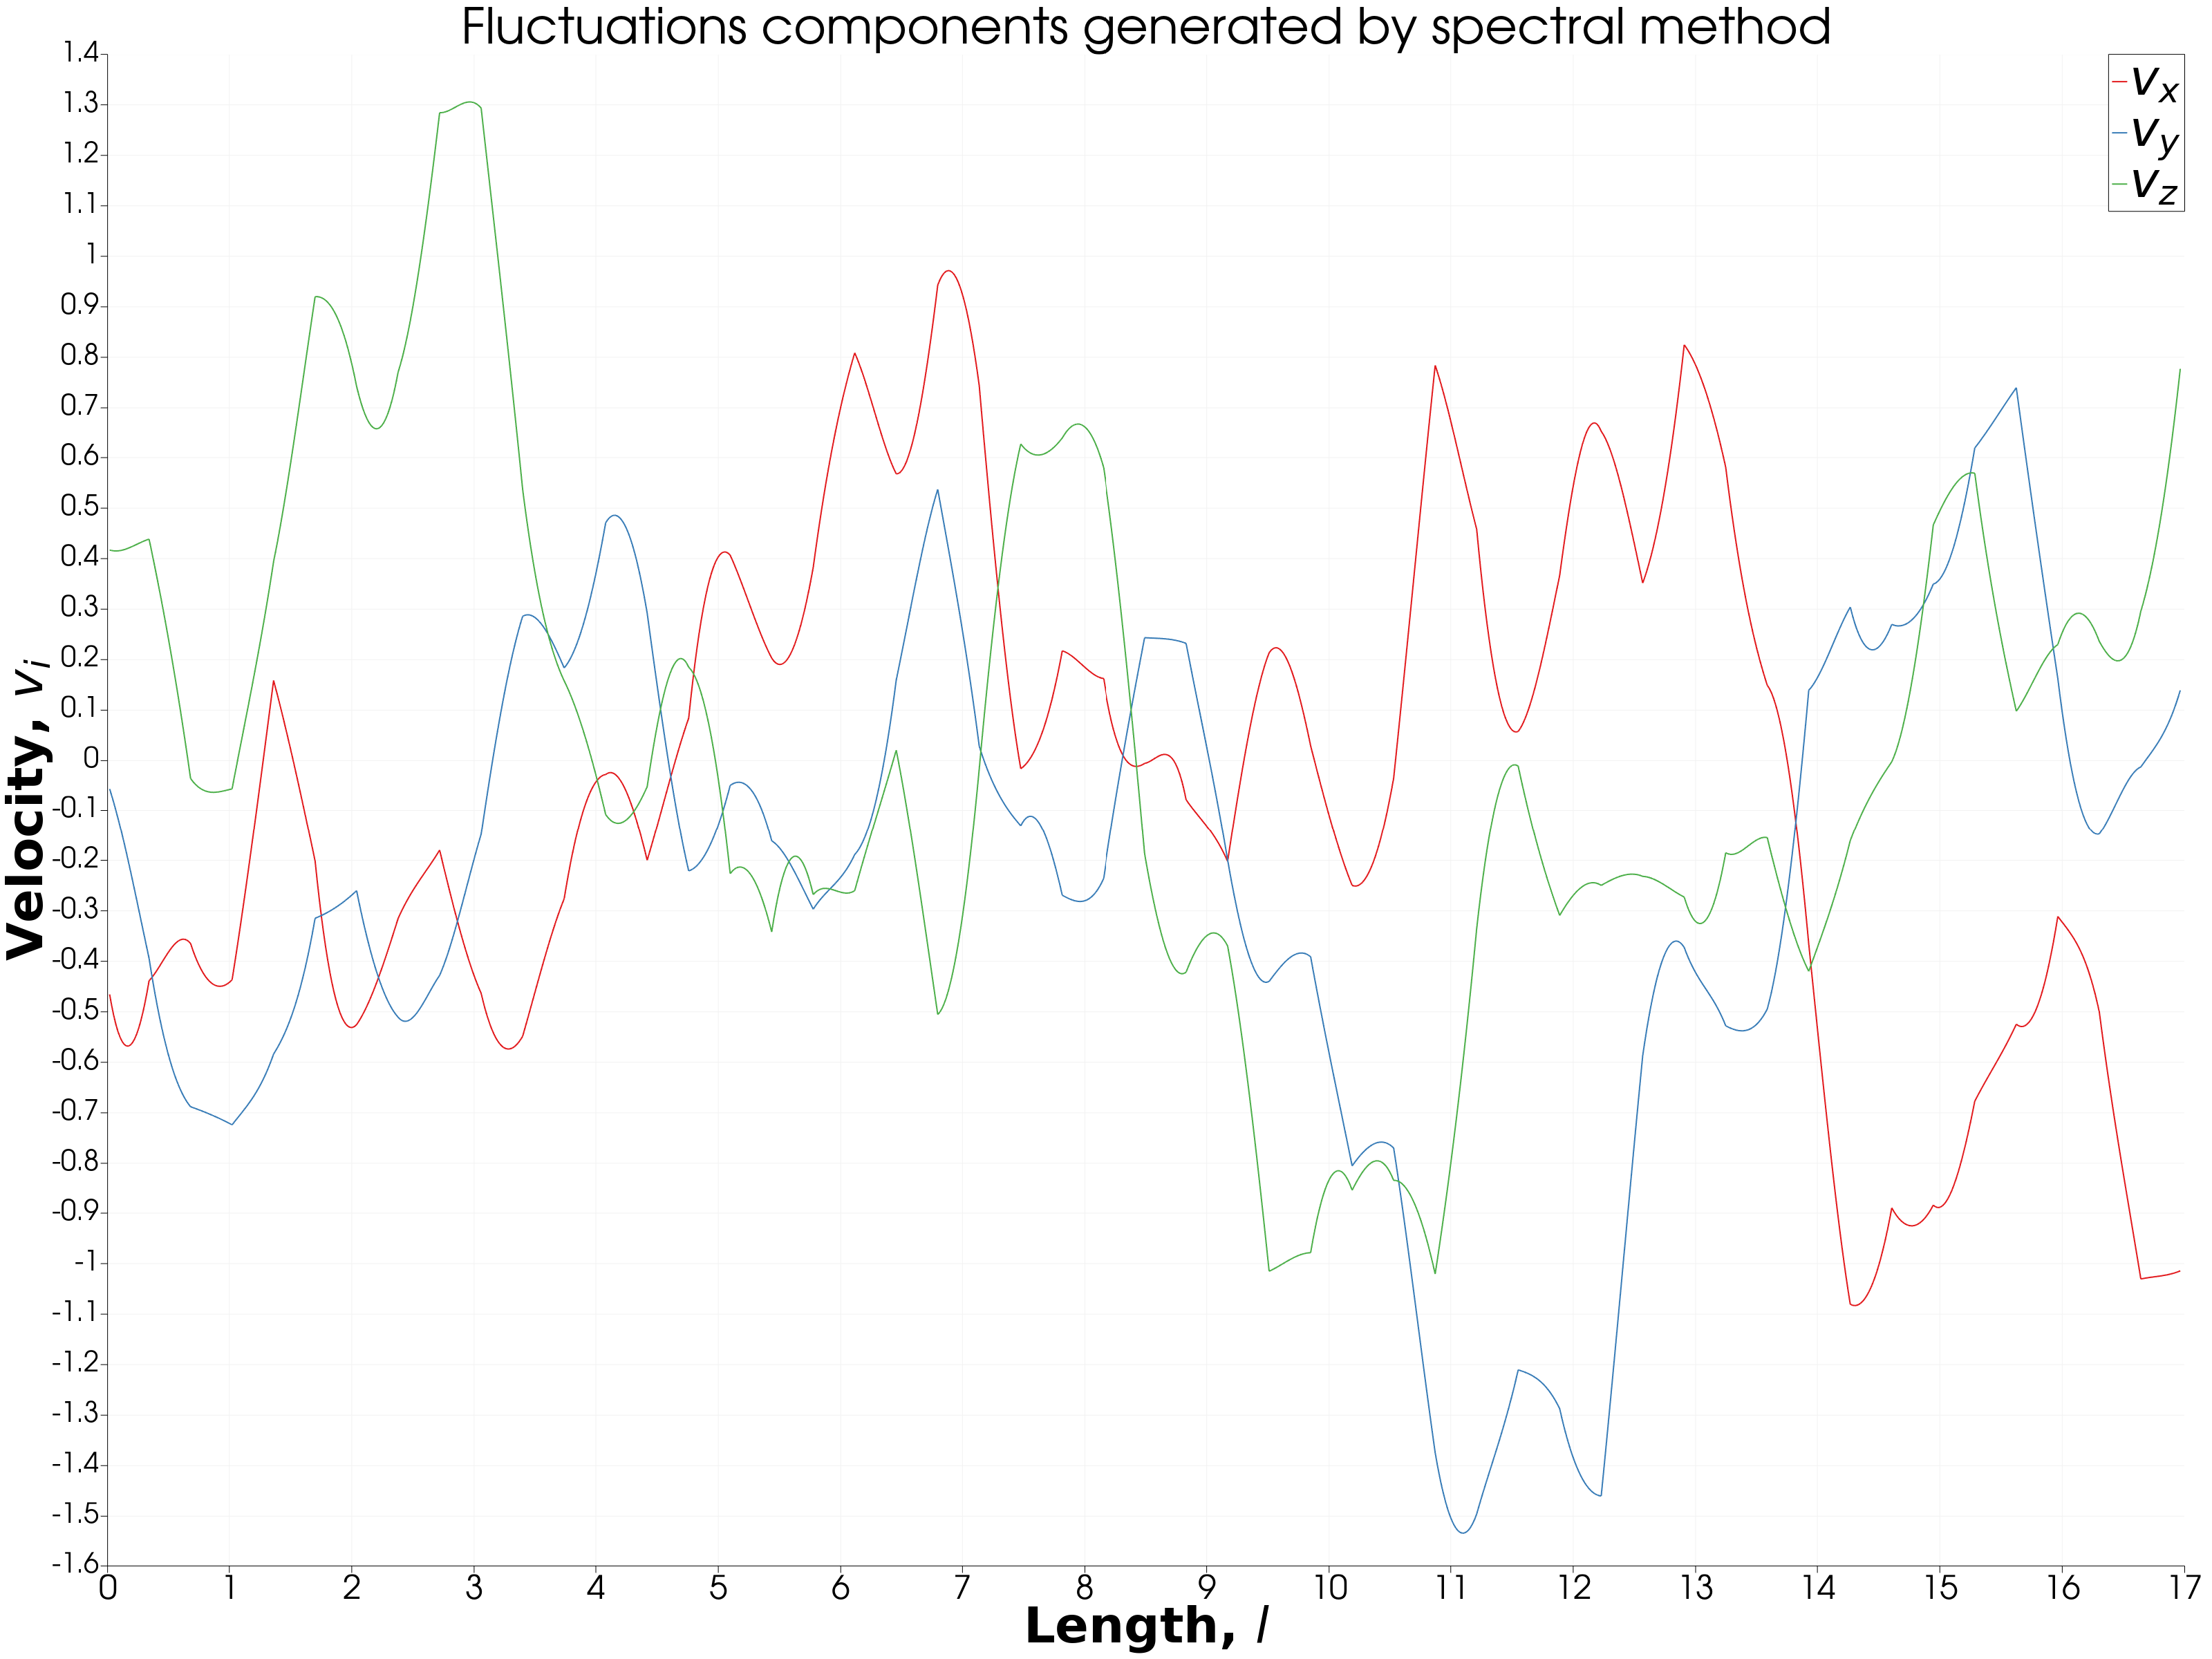
\includegraphics [width=0.8\linewidth] {images/spectral/velocity_components.png}
    \caption{Колебания компонент флуктуаций вдоль диагонали куба} 
    \label{img:spectral_method_velocity_components_along_diagonal}  
\end{figure}

\begin{figure}[ht] 
    \center
    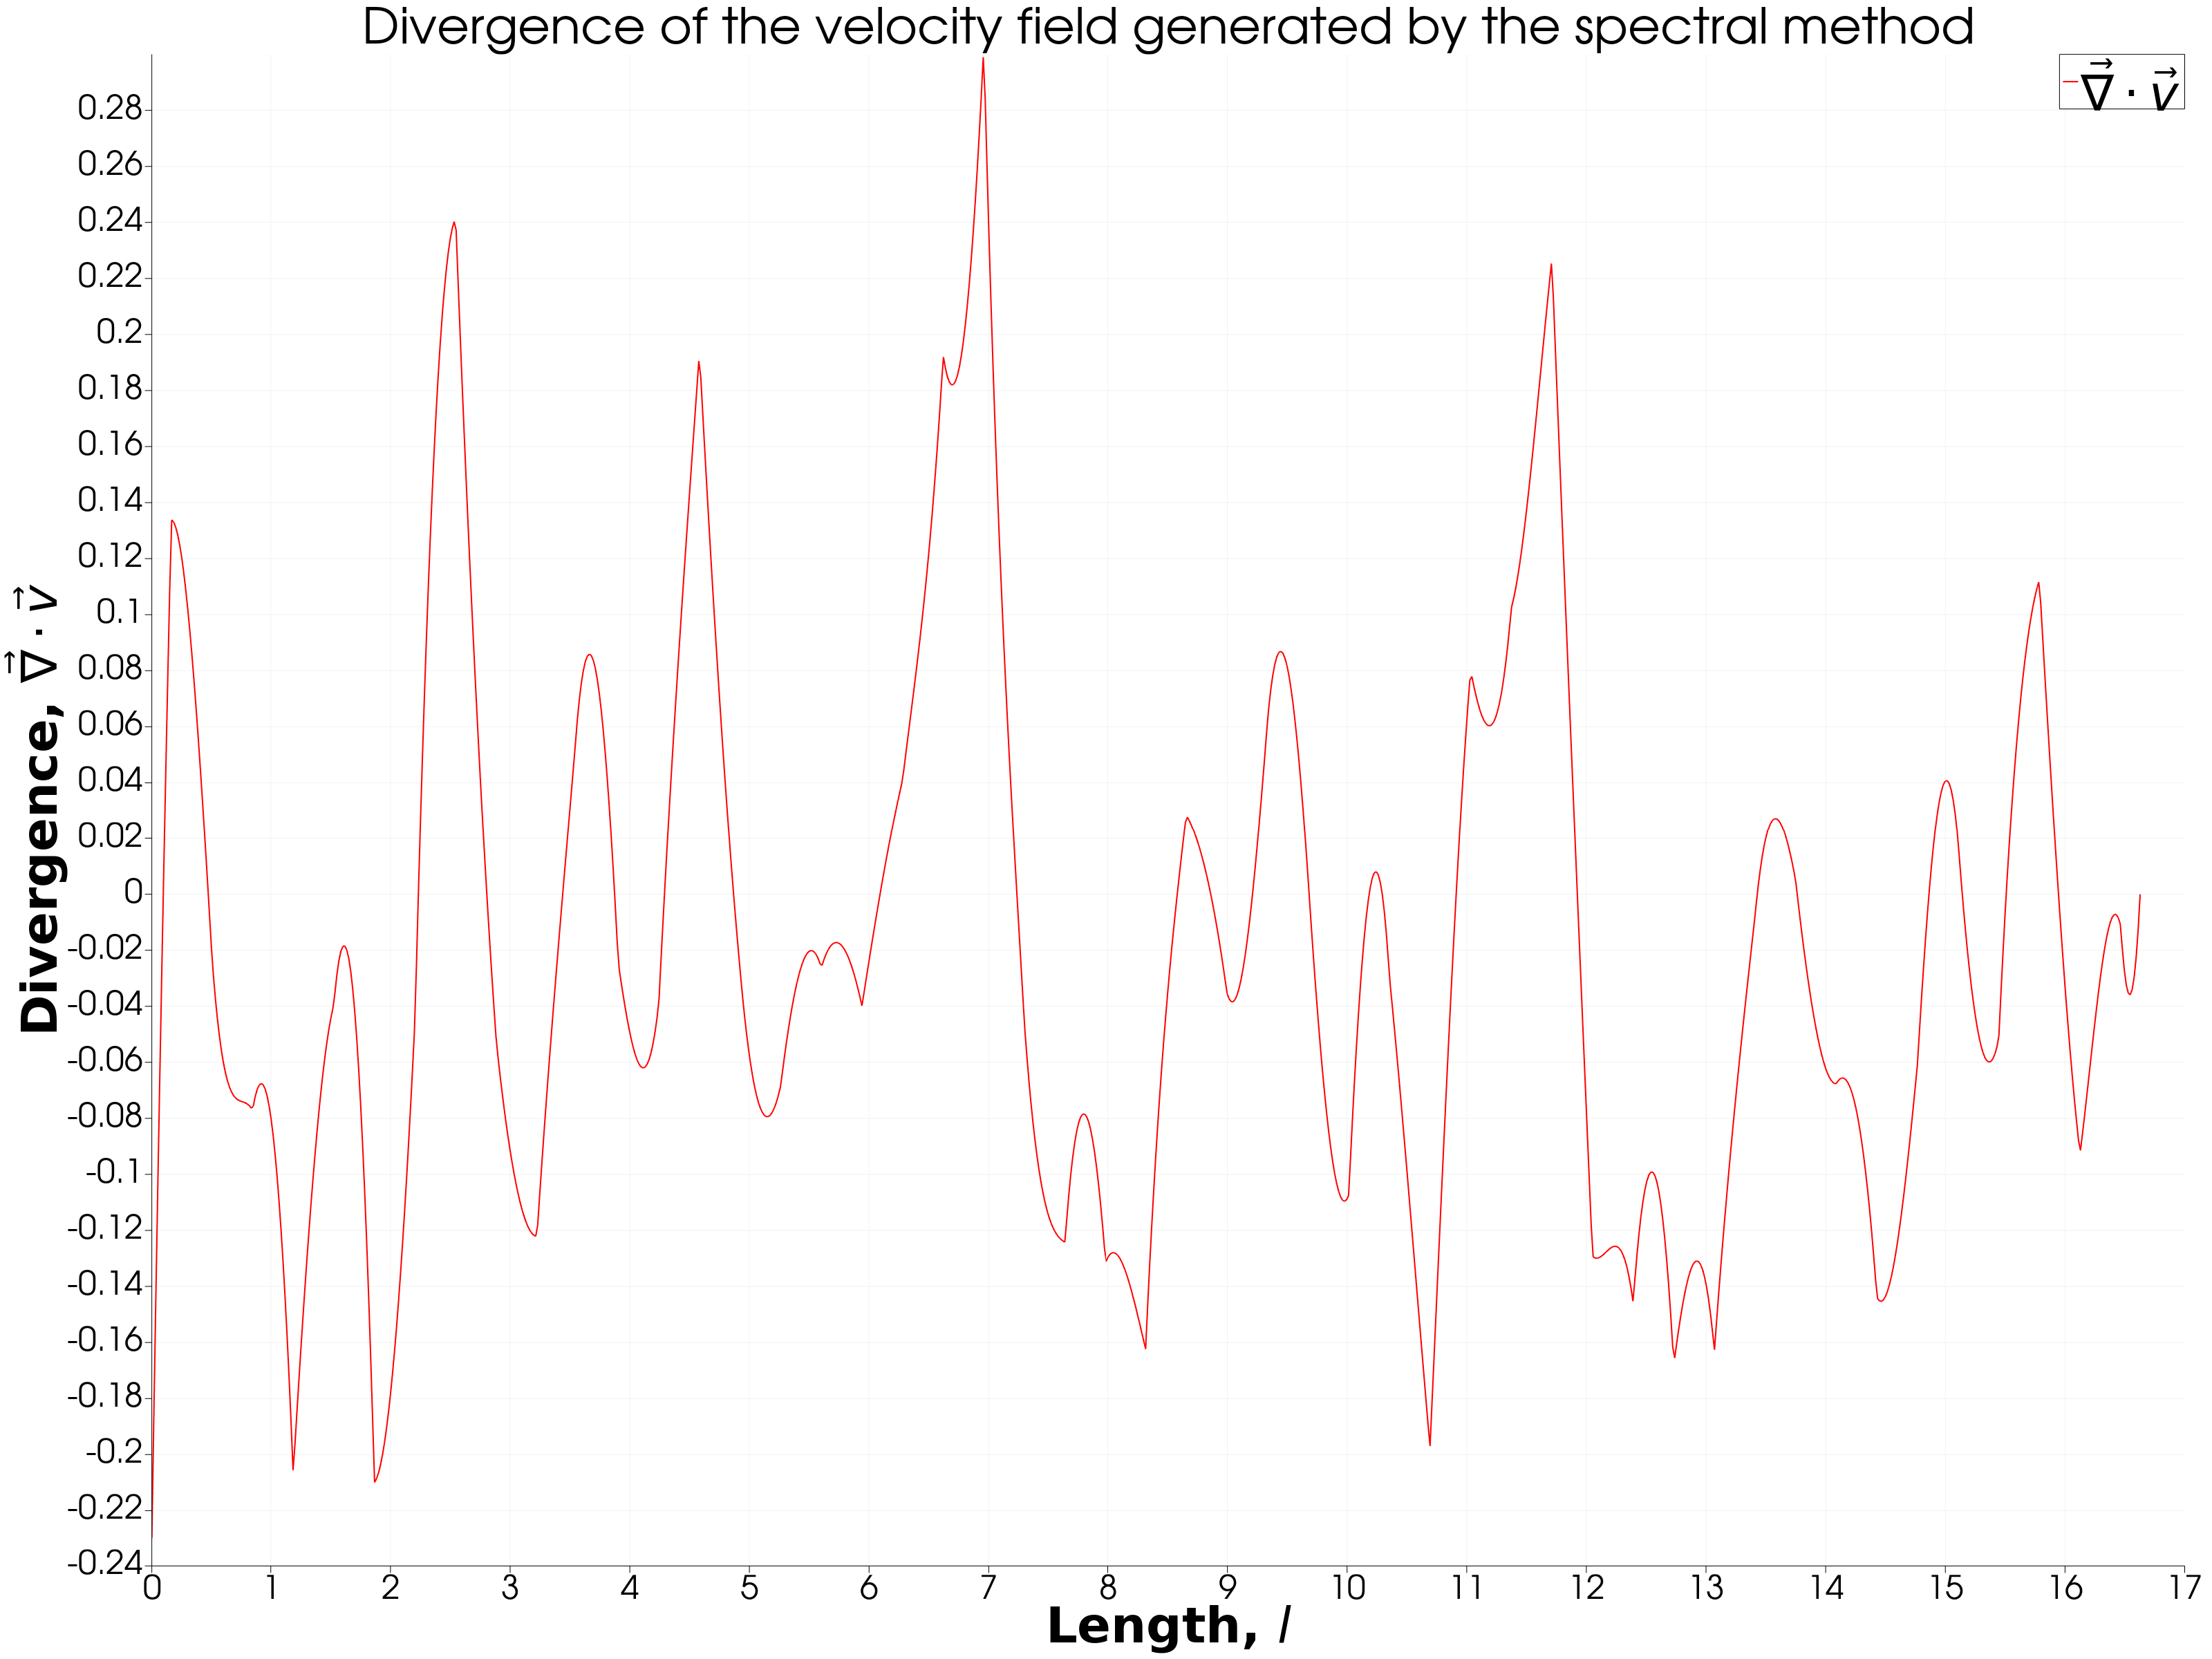
\includegraphics [width=0.8\linewidth] {images/spectral/divergence.png}
    \caption{Сумма $\frac{\partial v_x}{\partial x} + \frac{\partial v_y}{\partial y} + \frac{\partial v_z}{\partial z}$ вдоль диагонали куба} 
    \label{img:spectral_method_velocity_field_divergence}  
\end{figure}

Как мы может видеть, хоть амплитуды отклонений имеют не большую амплитуду, конечное поле не является тождественно удовлетворяющим уравнению неразрывности. Связано это может быть в первую очередь с аппроксимацией скоростей на сетке. Среднее значение отклонения на сетке $\mathbb{E}(\vec \nabla \cdot \vec{v}) \approx 1.108 \cdot 10^{-6}$, средние значения $\langle v_x \rangle> \approx 0.0265$, $\langle v_z \rangle \approx -0,0878217$, $\langle v_z \rangle \approx -0,0626564$, осреднение проводилось по объёму всё вычислительной области.

% ---------- %
%  CHAPTER 4
% ---------- %
 
\chapter{Валидация стохастического метода генерации синтетической турбулентности} \label{chapt5}
Перед использованием метода стохастического моделирования необходимо оценить влияние параметров данного метода. В отличие от спектральных методов, смысл проверки параметров можно назвать в данном случае другим. От таких параметров как допуск по величине ковариации и количеству собственных значений, зависит не столько конечный результат, сколько требуемая вычислительная мощность. На примере одномерного моделирования рассмотрим влияние параметров числа находимых собственных значений и выбираемым значениям амплитуд ковариации. Число собственных чисел входит в конечную формулу для генерации случайных чисел с заданной корреляцией, в силу того, что используется в итоге конечное число случайных чисел, необходимо проследить как влияет на решение их число. Также при нахождении собственных чисел появлялись отрицательные собственные числа, что является нежелательным эффектом. Связано это может быть с упомянутым в главе \ref{chapt2} свойством неотрицательной определённости матрицы ковариаций. Из этого не следует возможность в появлении отрицательных собственных чисел, но из-за машинного шума компоненты матрицы ковариации могут быть меньше 0, когда они равны в точности 0 и побудить появление отрицательных собственных чисел. Также необходимо учесть, что метод нахождения собственных чисел построен на итерационном процессе, в котором также может накапливаться ошибка.

При рассмотрении допуска по величине ковариаций можно достаточно сильно сэкономить на заполненности матрица ковариаций, тем самым увеличив, например разбиение по сетке, либо увеличив хранимое число собственных чисел. Но это также влияет на коррелированность пар значений при случаях когда ковариация между ними равна 0. Также есть другая цена у допуска, больше значений матрицы ковариаций нулевые, хоть они и не хранятся в разреженной матрице, что как отмечалось выше, может спровоцировать появление отрицательных собственных чисел. В целом, можно использовать допуск одновременно исключая отрицательные собственные числа.

Как говорилось выше, для оценки влияния рассматриваемых параметров нужно было провести несколько вычислительных экспериментов. Число собственных чисел варьировалось от 100 до 600 с шагом 50, допуск по амплитудам ковариации варьировался от 0\% до 5\% с шагов в 1\%. Критерием удовлетворения заданным параметрам являться близость ковариационной функции построенного поля к задаваемой. Задаваемая ковариационная функция является по определению Фурье образом от функции турбулентного спектра, задаваемого аналитически.

Рассмотрим сравнение между полученными данными для всех случаев в срезах по осям $x, y, z$ (линия проходит через центр куба, совпадающий с началом координат) и диагонали между точками $\{-5, -5, -5\}$ и $\{5, 5, 5\}$ внутри куба со стороной равной 10, и числом разбиений 21 как для пространства Фурье и ковариационной функции, так и для разбиения реального пространства. Пространственная ковариация рассчиталась с использованием набора из 1000 генераций для одного набора собственных значений. Все рассматриваемые сечения проходят через центр, так как вид ковариационной функции близок к виду Гауссовой кривой либо кривой Лоренца с пиками в центре координат.

Как упоминалось ранее, в общем случае, метод может иметь в наборе собственных значений также отрицательные собственные числа. Их число зависит не только от собираемой матрицы ковариаций, но также и от параметров оборачивания этой матрицы. Без ограничений по числу итераций, а также с алгоритмом прохода по наибольшим собственных значениям среди 9200 собственных чисел (совпадает с размерностью матрицы ковариаций) около 200 являются отрицательными, это около $2\%$ от общего числа собственных чисел. Хоть это число и мало, необходимо оценить, сколько собственных чисел стоит брать для хорошего удовлетворения ковариационной функции. Число отрицательных собственных чисел также может расти/уменьшаться с изменением как параметров сетки, так и в целом параметров спектра, итерационного метода и самого базиса метода стохастического моделирования (например при использовании кокригинга). Хоть $2\%$ сама по себе достаточно малая величина, может оказаться так, что необходимо брать полный набор собственных значений и векторов для генерации поля турбулентности.

%
% Обрезание 0%
%
\begin{figure}[!ht]
    \center{

        \subcaptionbox[List-of-Figures entry]{диагональ\label{img:comparison_covcut0_diag}} 
        {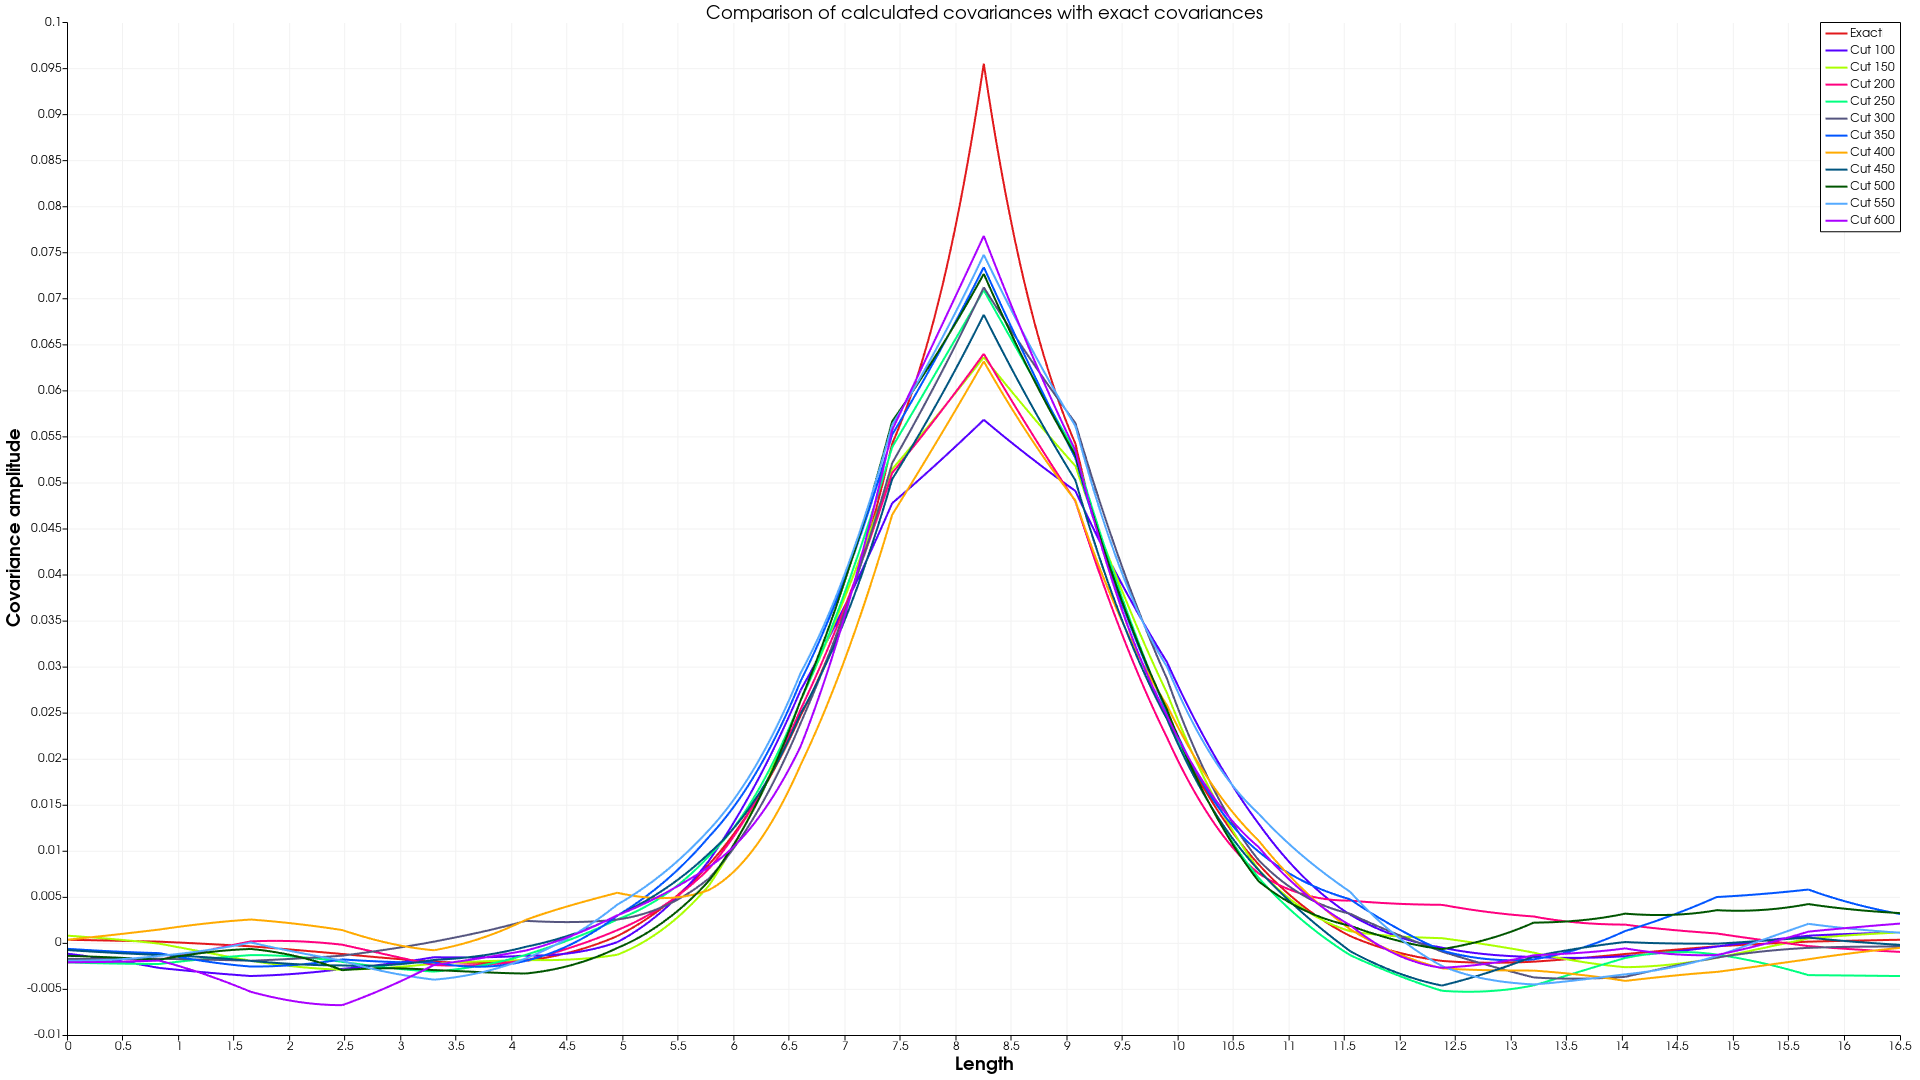
\includegraphics[width=0.45\linewidth]{comparison_covcut0_diag}}%
        \hfill
        \subcaptionbox{$x$ направление\label{img:comparison_covcut0_x}} 
        {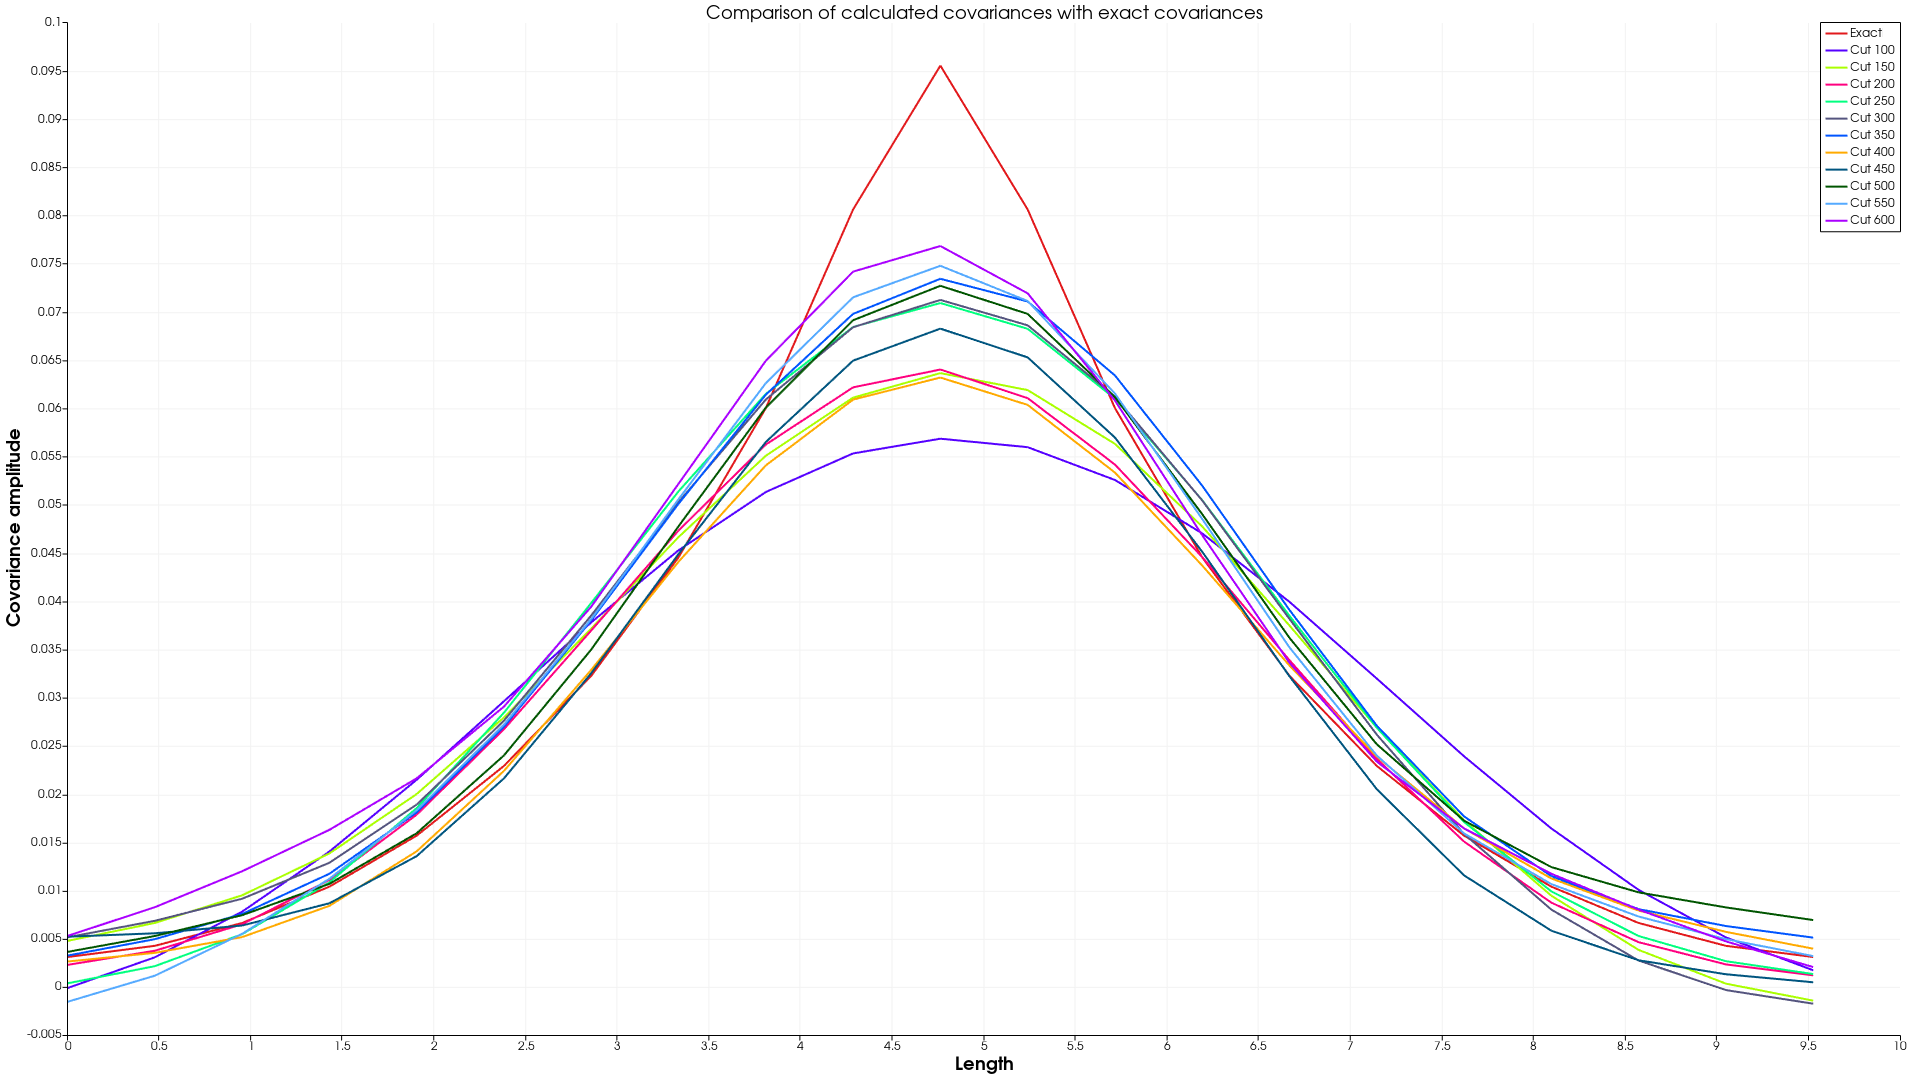
\includegraphics[width=0.45\linewidth]{comparison_covcut0_x}} \\

    }
    \center{

        \subcaptionbox[List-of-Figures entry]{$y$ направление\label{img:comparison_covcut0_y}} 
        {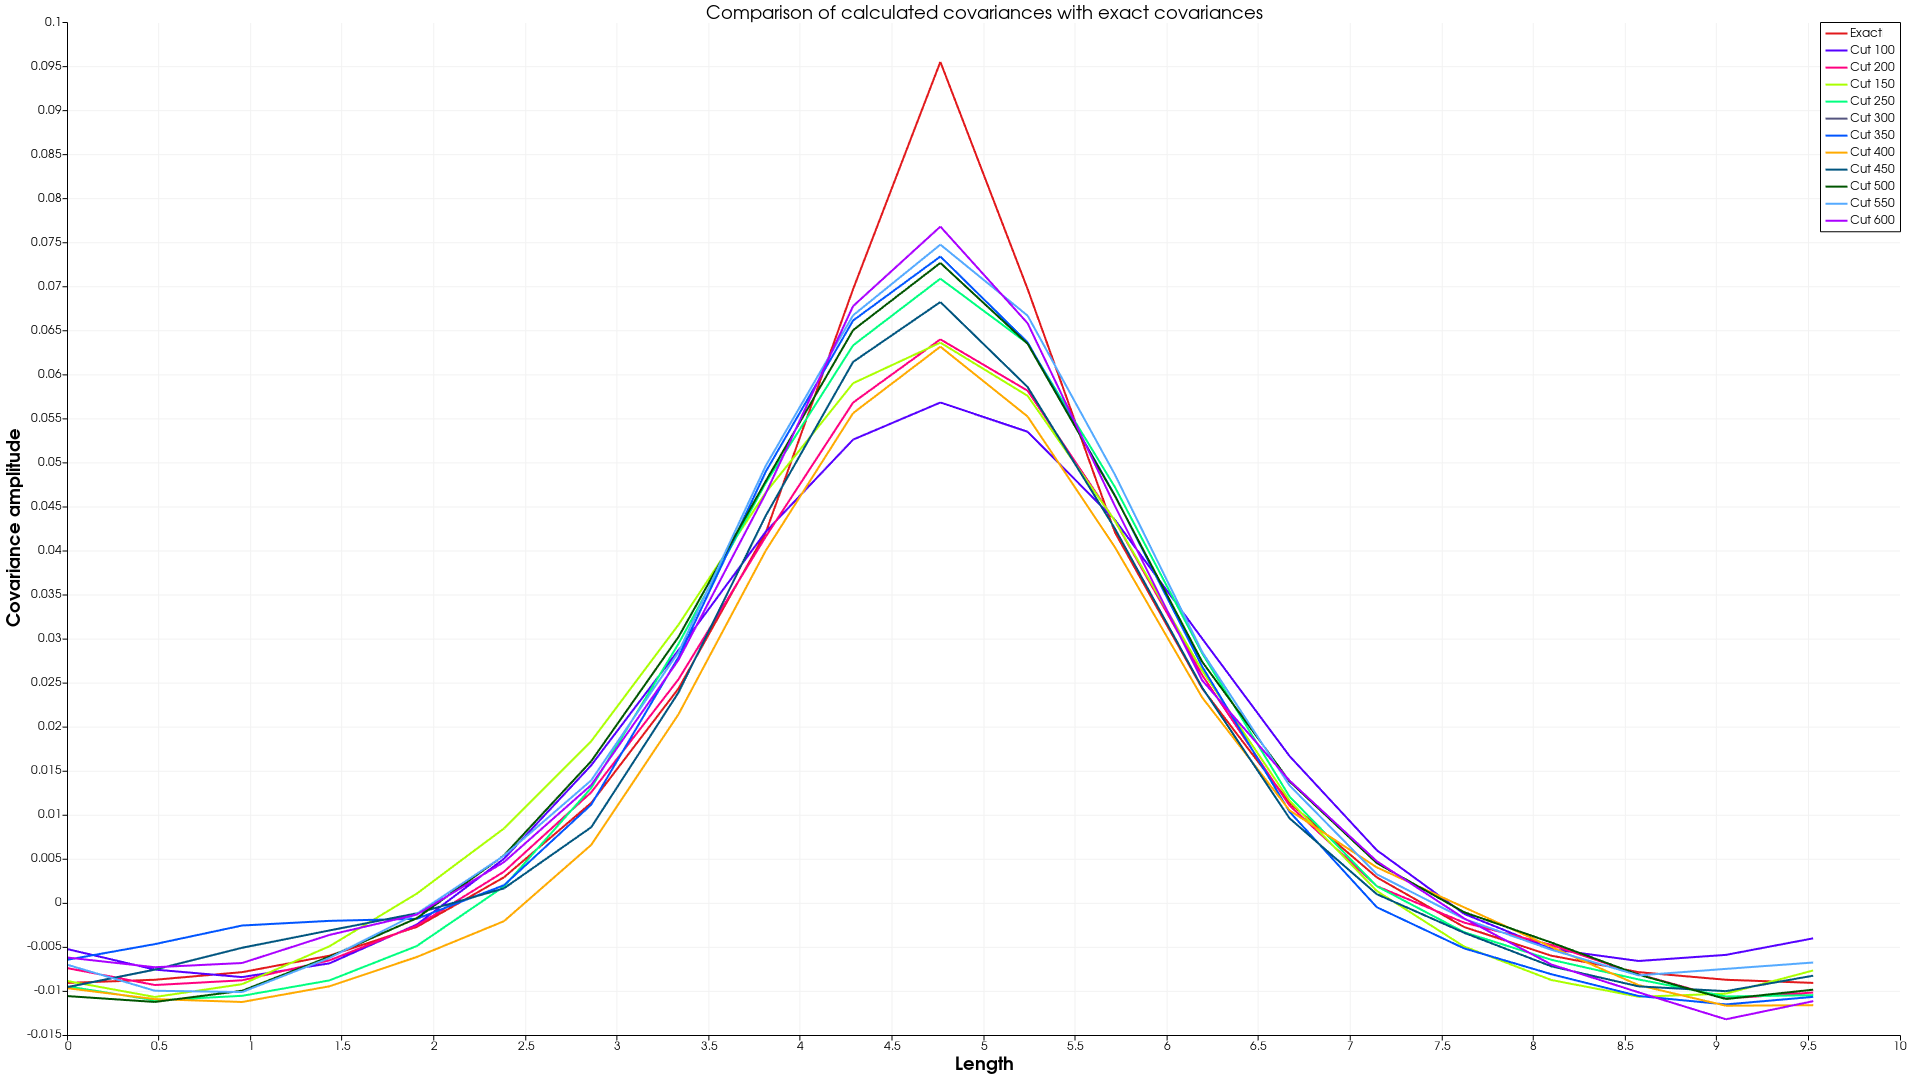
\includegraphics[width=0.45\linewidth]{comparison_covcut0_y}}%
        \hfill
        \subcaptionbox{$z$ направление\label{img:comparison_covcut0_z}} 
        {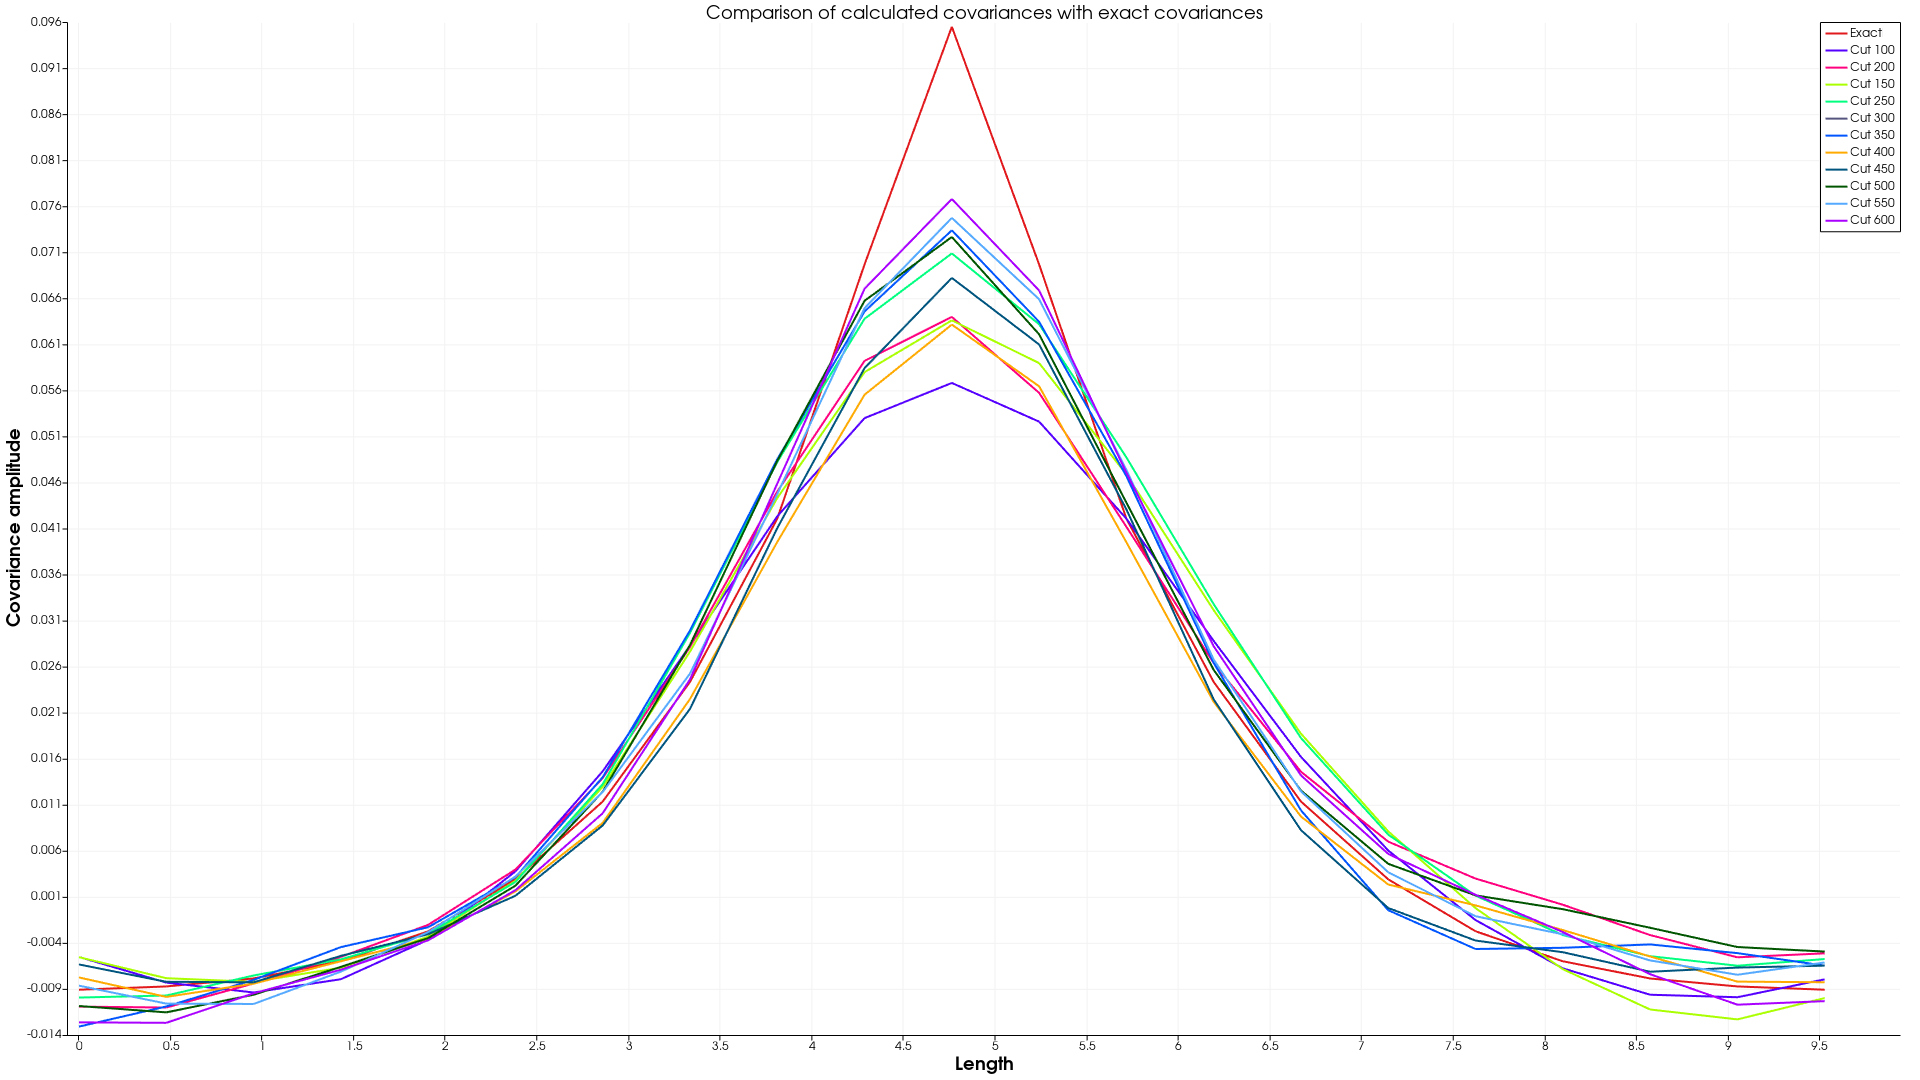
\includegraphics[width=0.45\linewidth]{comparison_covcut0_z}}

    }
    
    \onehalfspacing{Сравнение ковариацинной функции, допуск 0\%, для направлений а) вдоль диагонали, б) вдоль оси $x$, в) вдоль оси $y$, г) вдоль оси $z$}
    \caption{Сравнение ковариационной функции для допуска по амплитуде ковариаций в 0\% для различных направлений в рассматриваемой области}
    \label{img:covcut_0_comparison}  
\end{figure}
%
% Обрезание 1%
%
\begin{figure}[!ht]
    \center{
        \subcaptionbox[List-of-Figures entry]{диагональ\label{img:comparison_covcut1_diag}} 
        {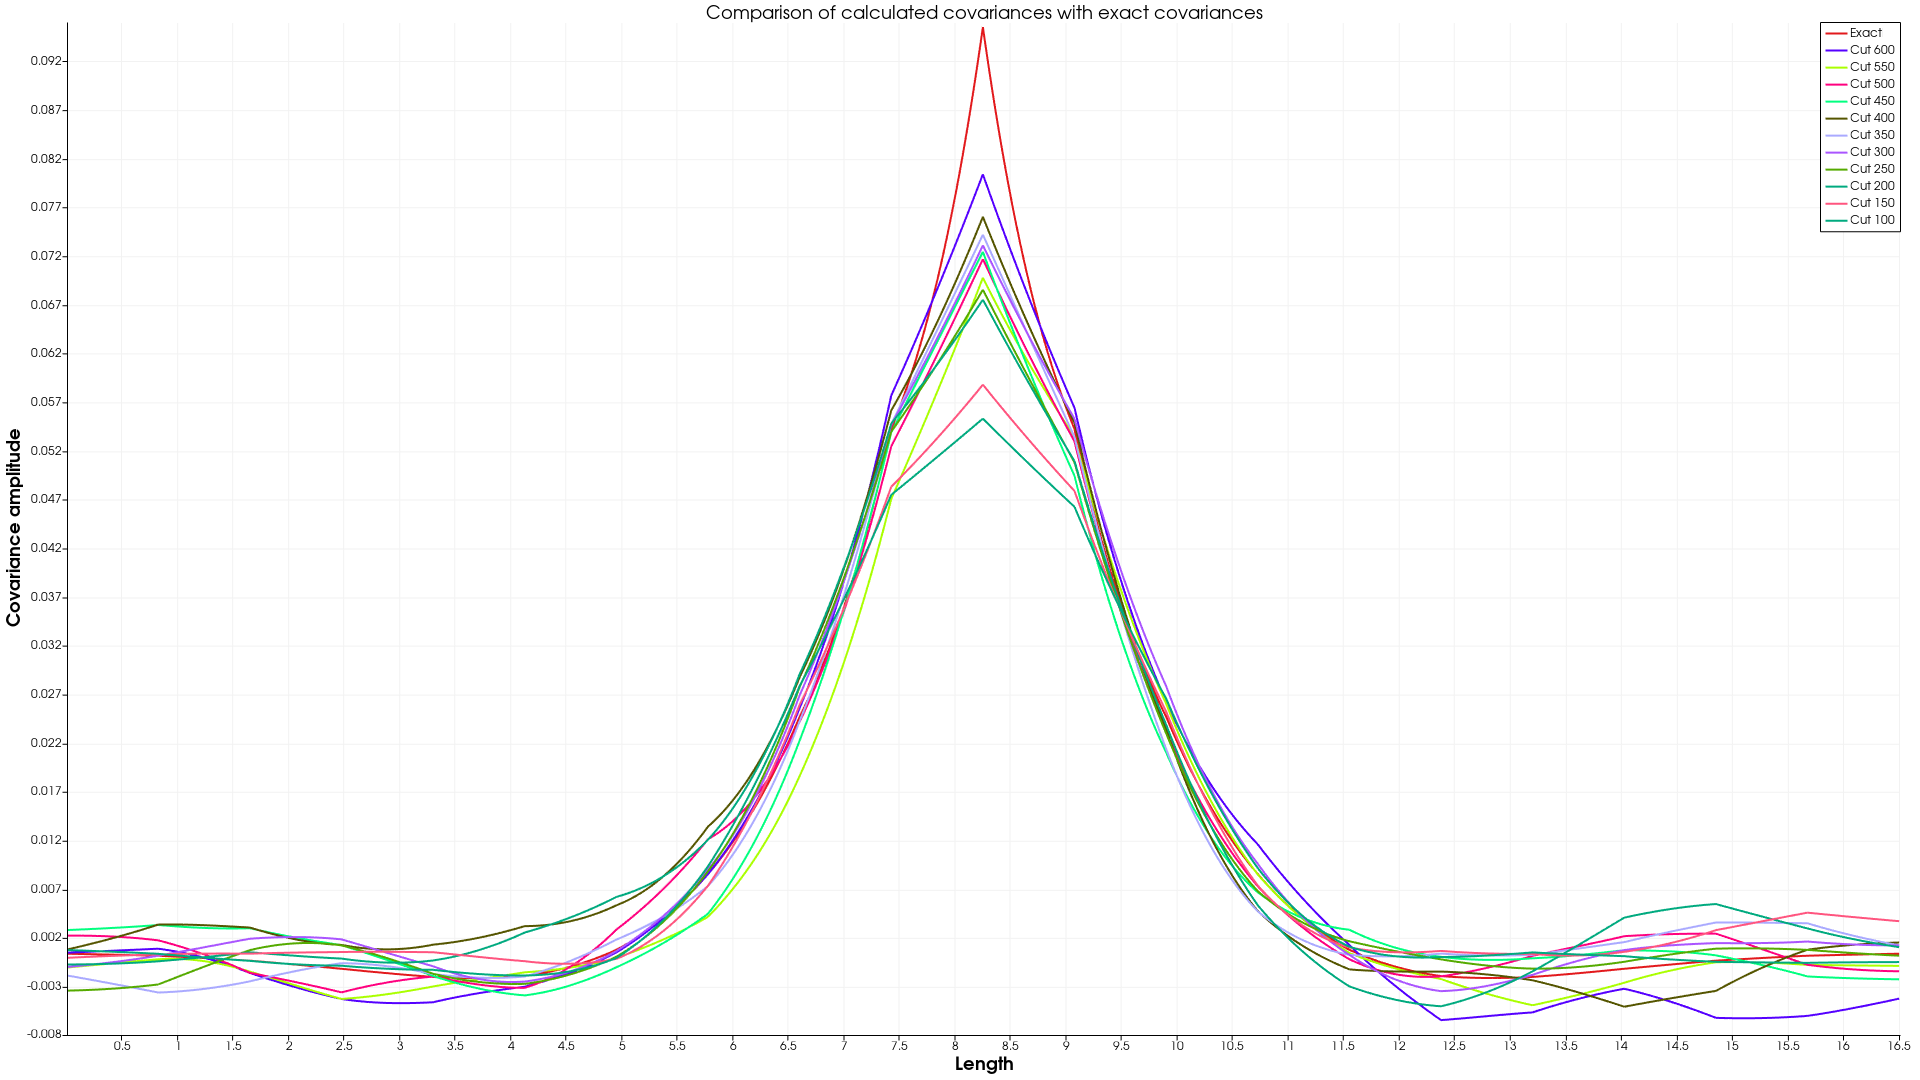
\includegraphics[width=0.45\linewidth]{comparison_covcut1_diag}}%
        \hfill
        \subcaptionbox{$x$ направление\label{img:comparison_covcut1_x}} 
        {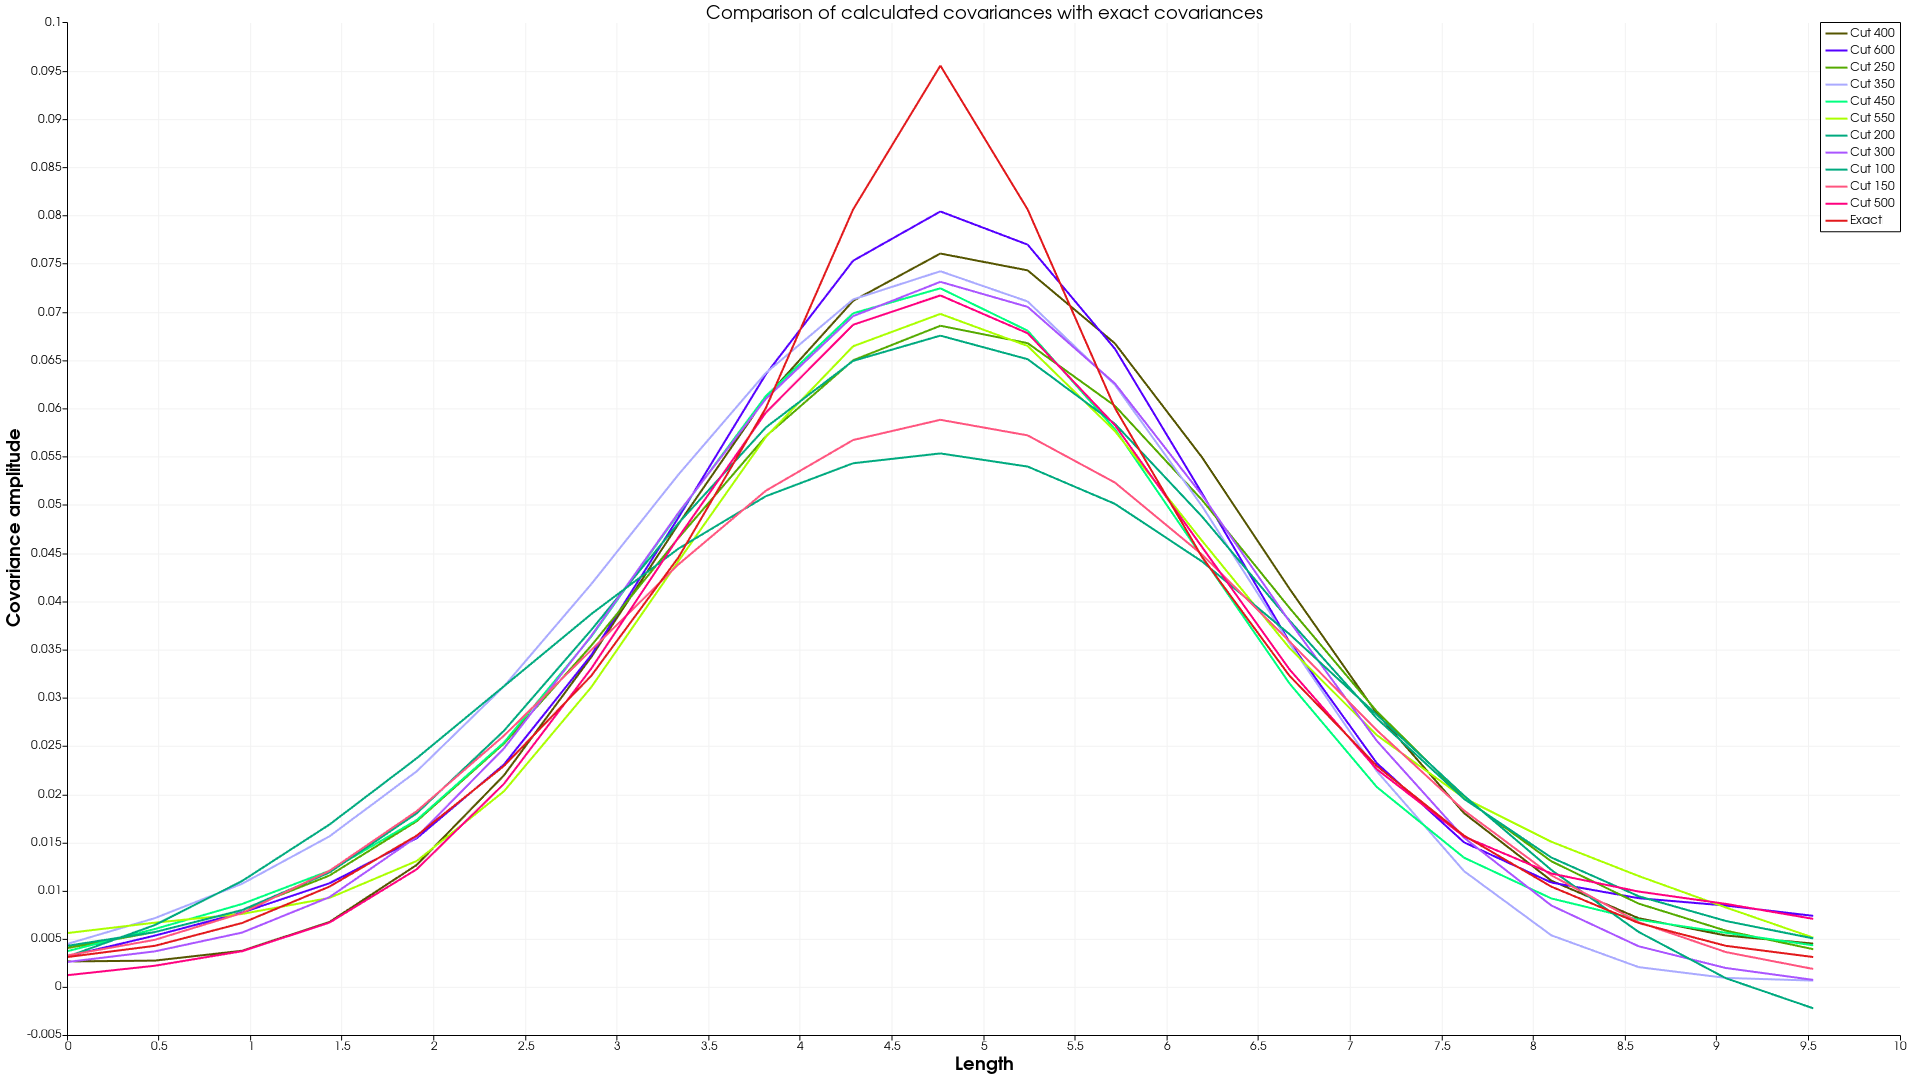
\includegraphics[width=0.45\linewidth]{comparison_covcut1_x}} \\

    }
    \center{    
        \subcaptionbox[List-of-Figures entry]{$y$ направление\label{img:comparison_covcut1_y}} 
        {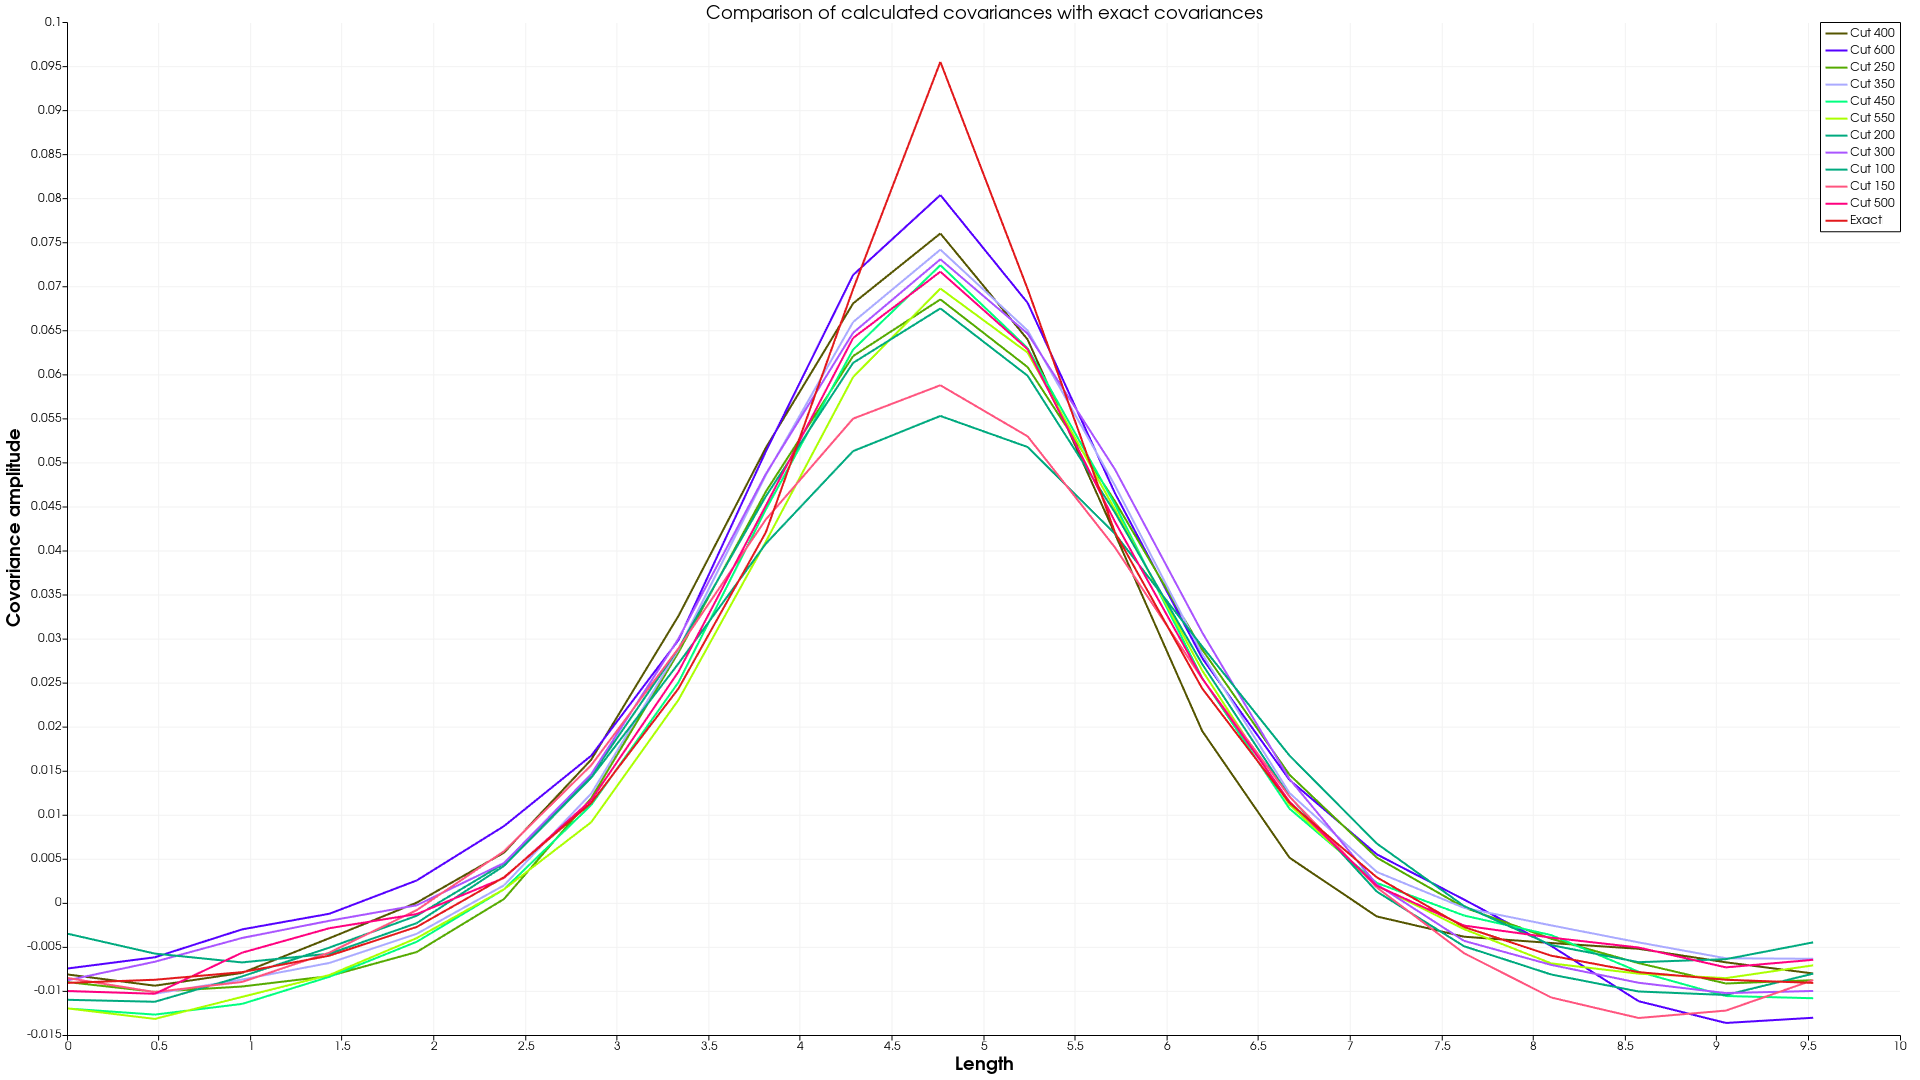
\includegraphics[width=0.45\linewidth]{comparison_covcut1_y}}%
        \hfill
        \subcaptionbox{$z$ направление\label{img:comparison_covcut1_z}} 
        {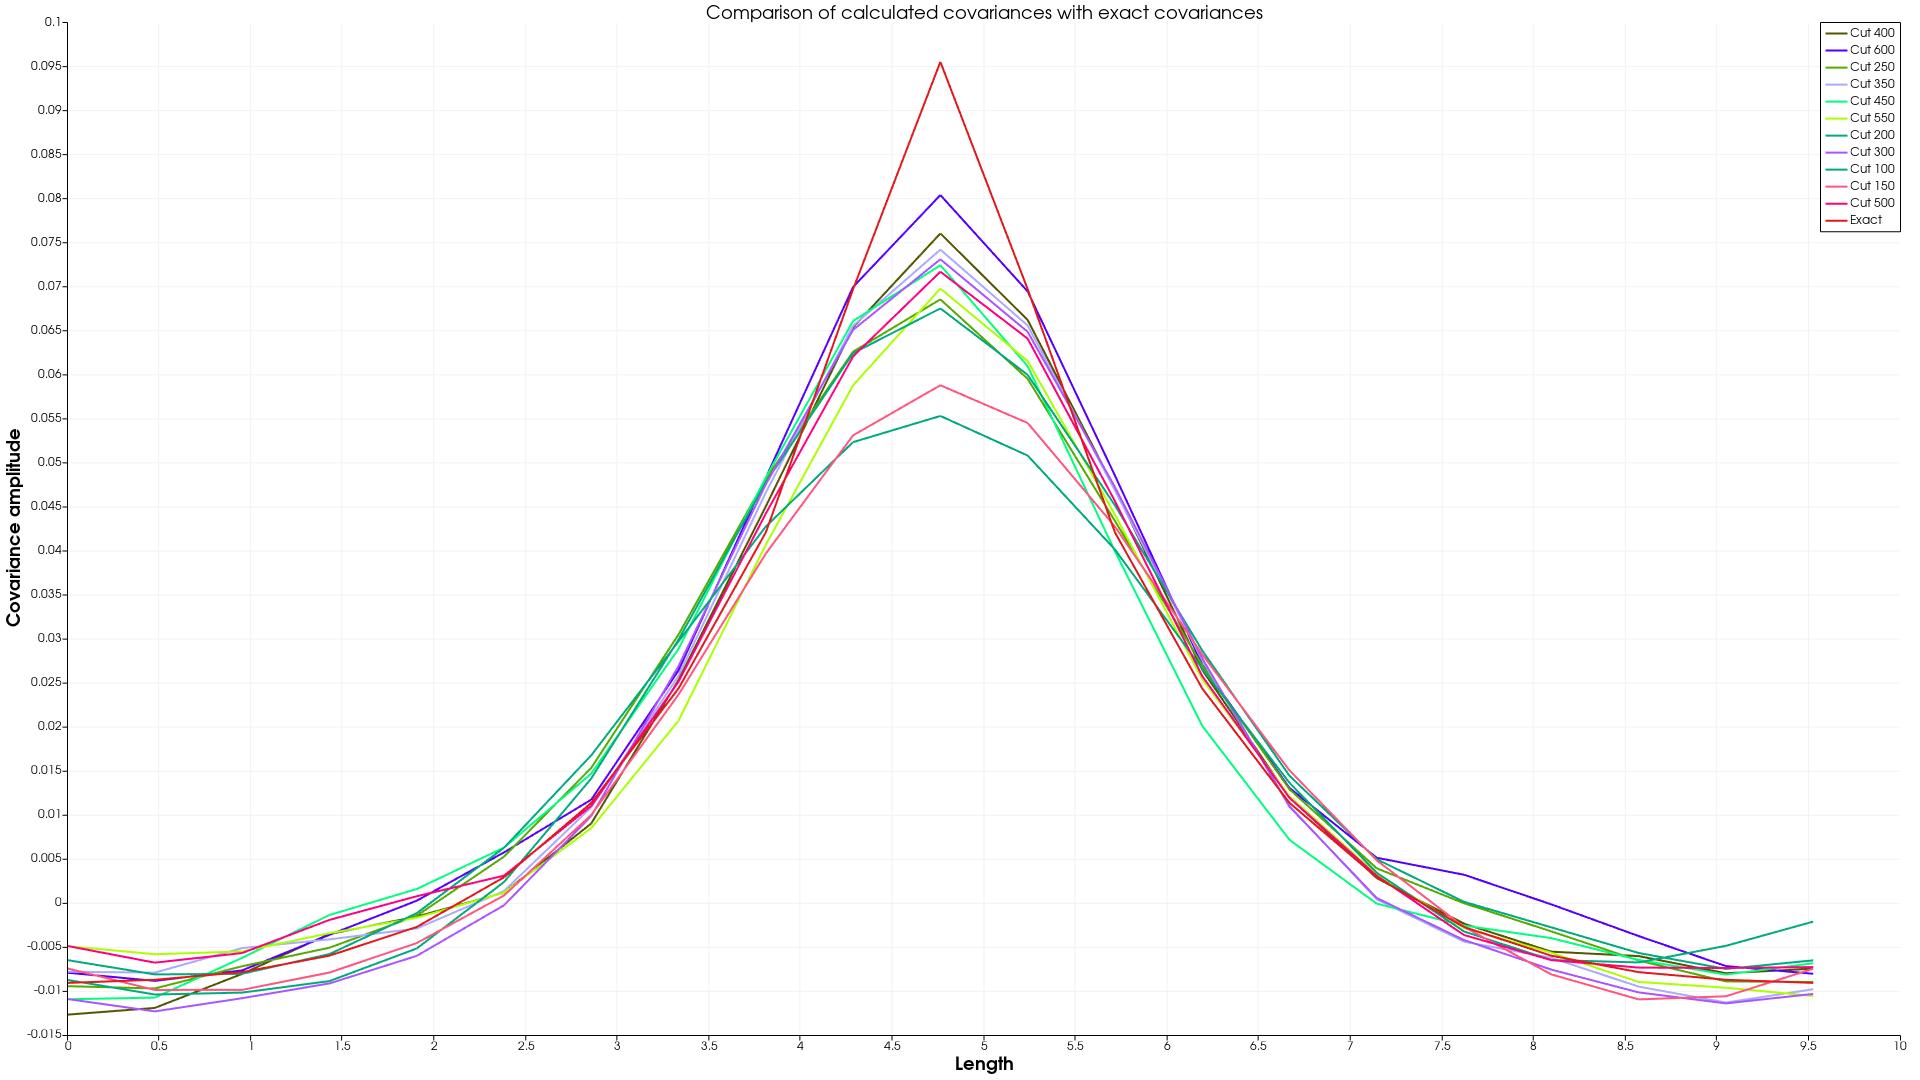
\includegraphics[width=0.45\linewidth]{comparison_covcut1_z}}
    }
    
    \onehalfspacing{Сравнение ковариацинной функции, допуск 1\%, для направлений а) вдоль диагонали, б) вдоль оси $x$, в) вдоль оси $y$, г) вдоль оси $z$}
    \caption{Сравнение ковариационной функции для допуска по амплитуде ковариаций в 1\% для различных направлений в рассматриваемой области}
    \label{img:covcut_1_comparison}  
\end{figure}
%
% Обрезание 2%
%
\begin{figure}[!ht]
    \center{
        \subcaptionbox[List-of-Figures entry]{диагональ\label{img:comparison_covcut2_diag}} 
        {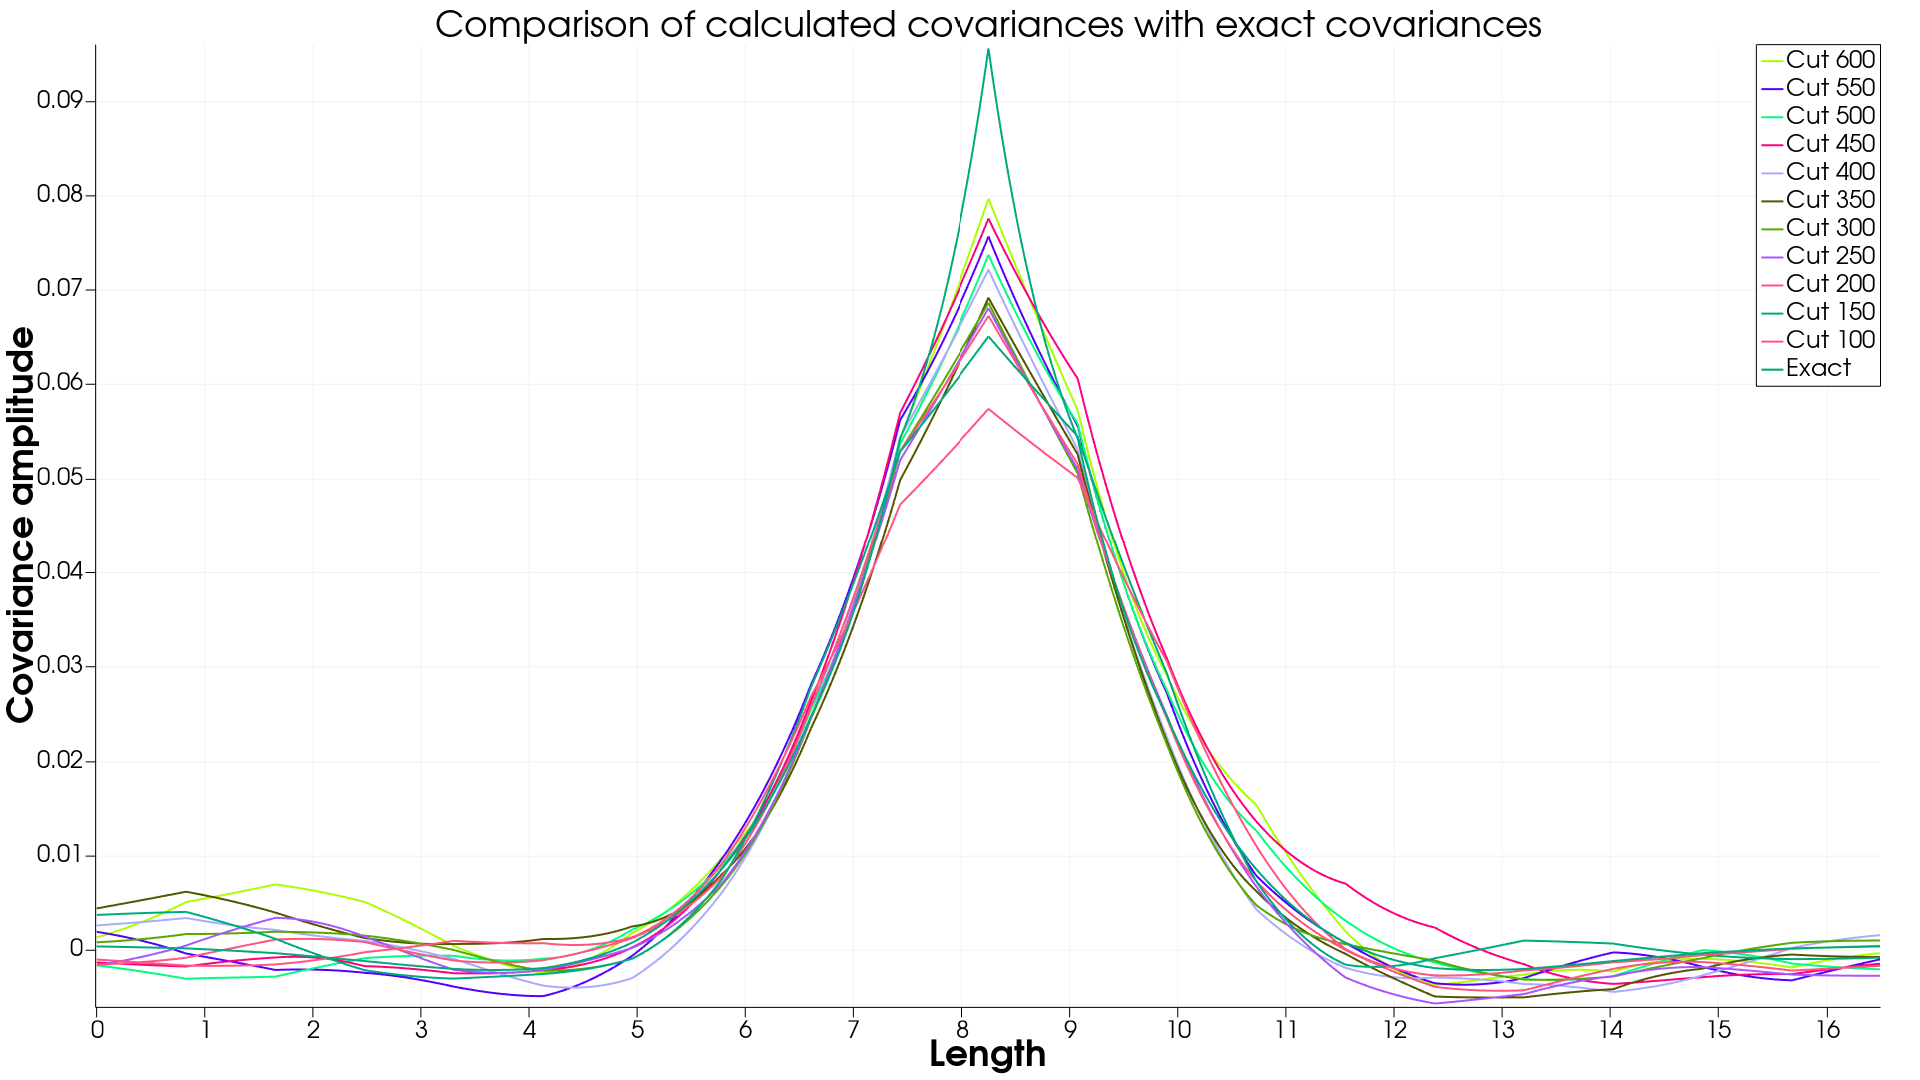
\includegraphics[width=0.45\linewidth]{comparison_covcut2_diag}}%
        \hfill
        \subcaptionbox{$x$ направление\label{img:comparison_covcut2_x}} 
        {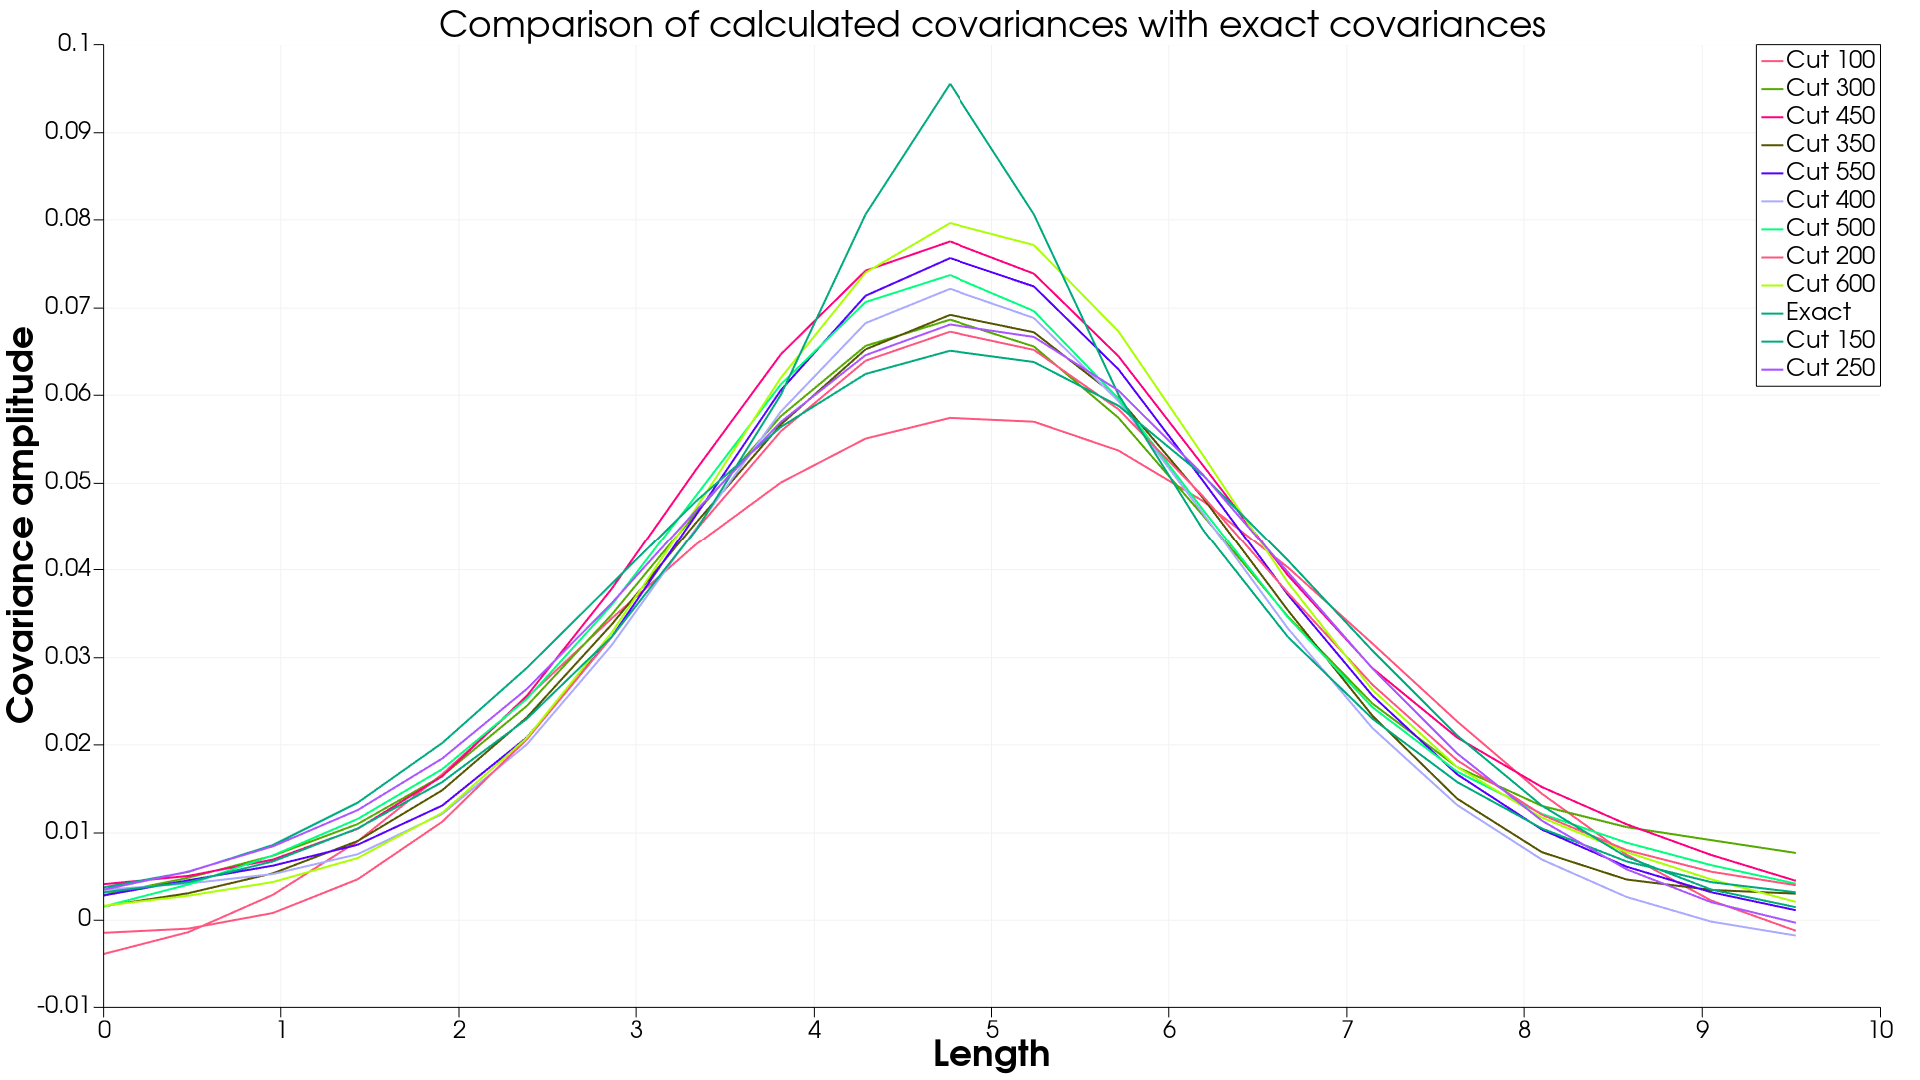
\includegraphics[width=0.45\linewidth]{comparison_covcut2_x}} \\
    }
    \center{
        \subcaptionbox[List-of-Figures entry]{$y$ направление\label{img:comparison_covcut2_y}} 
        {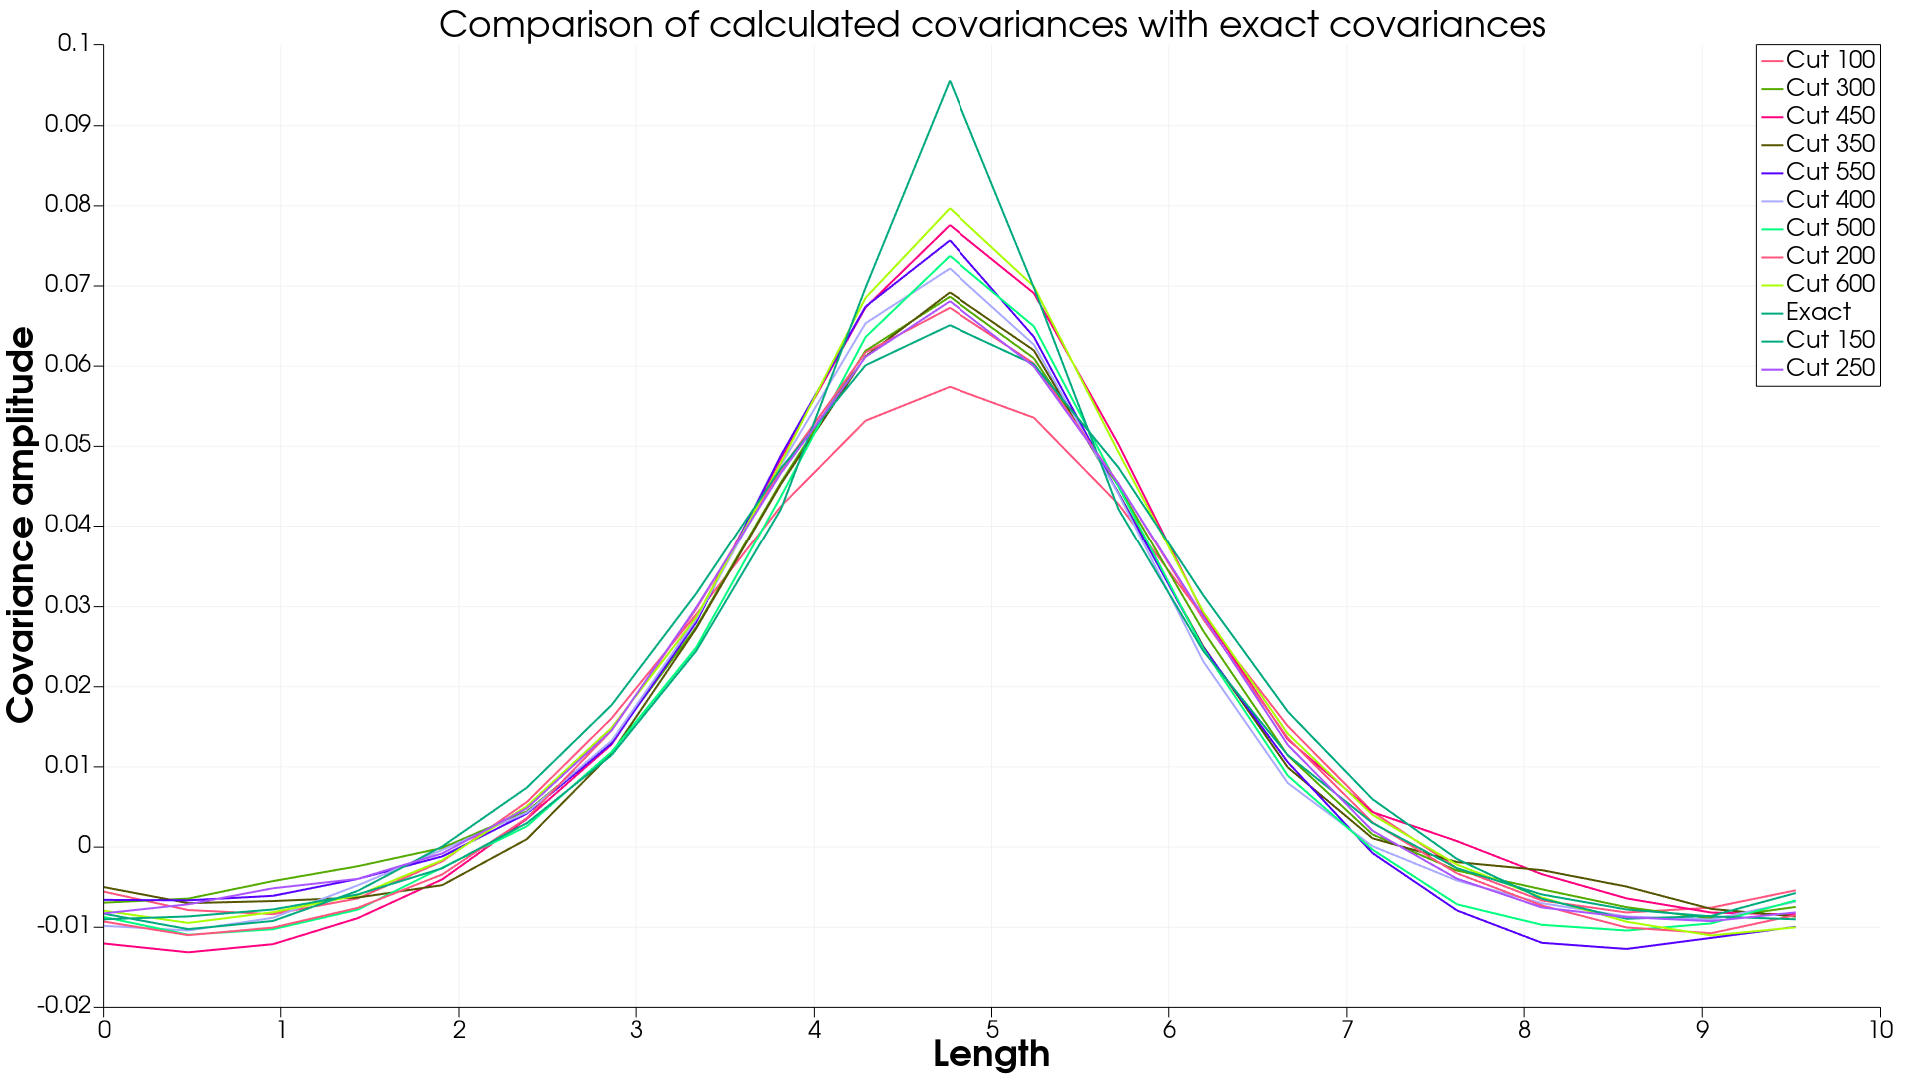
\includegraphics[width=0.45\linewidth]{comparison_covcut2_y}}%
        \hfill
        \subcaptionbox{$z$ направление\label{img:comparison_covcut2_z}} 
        {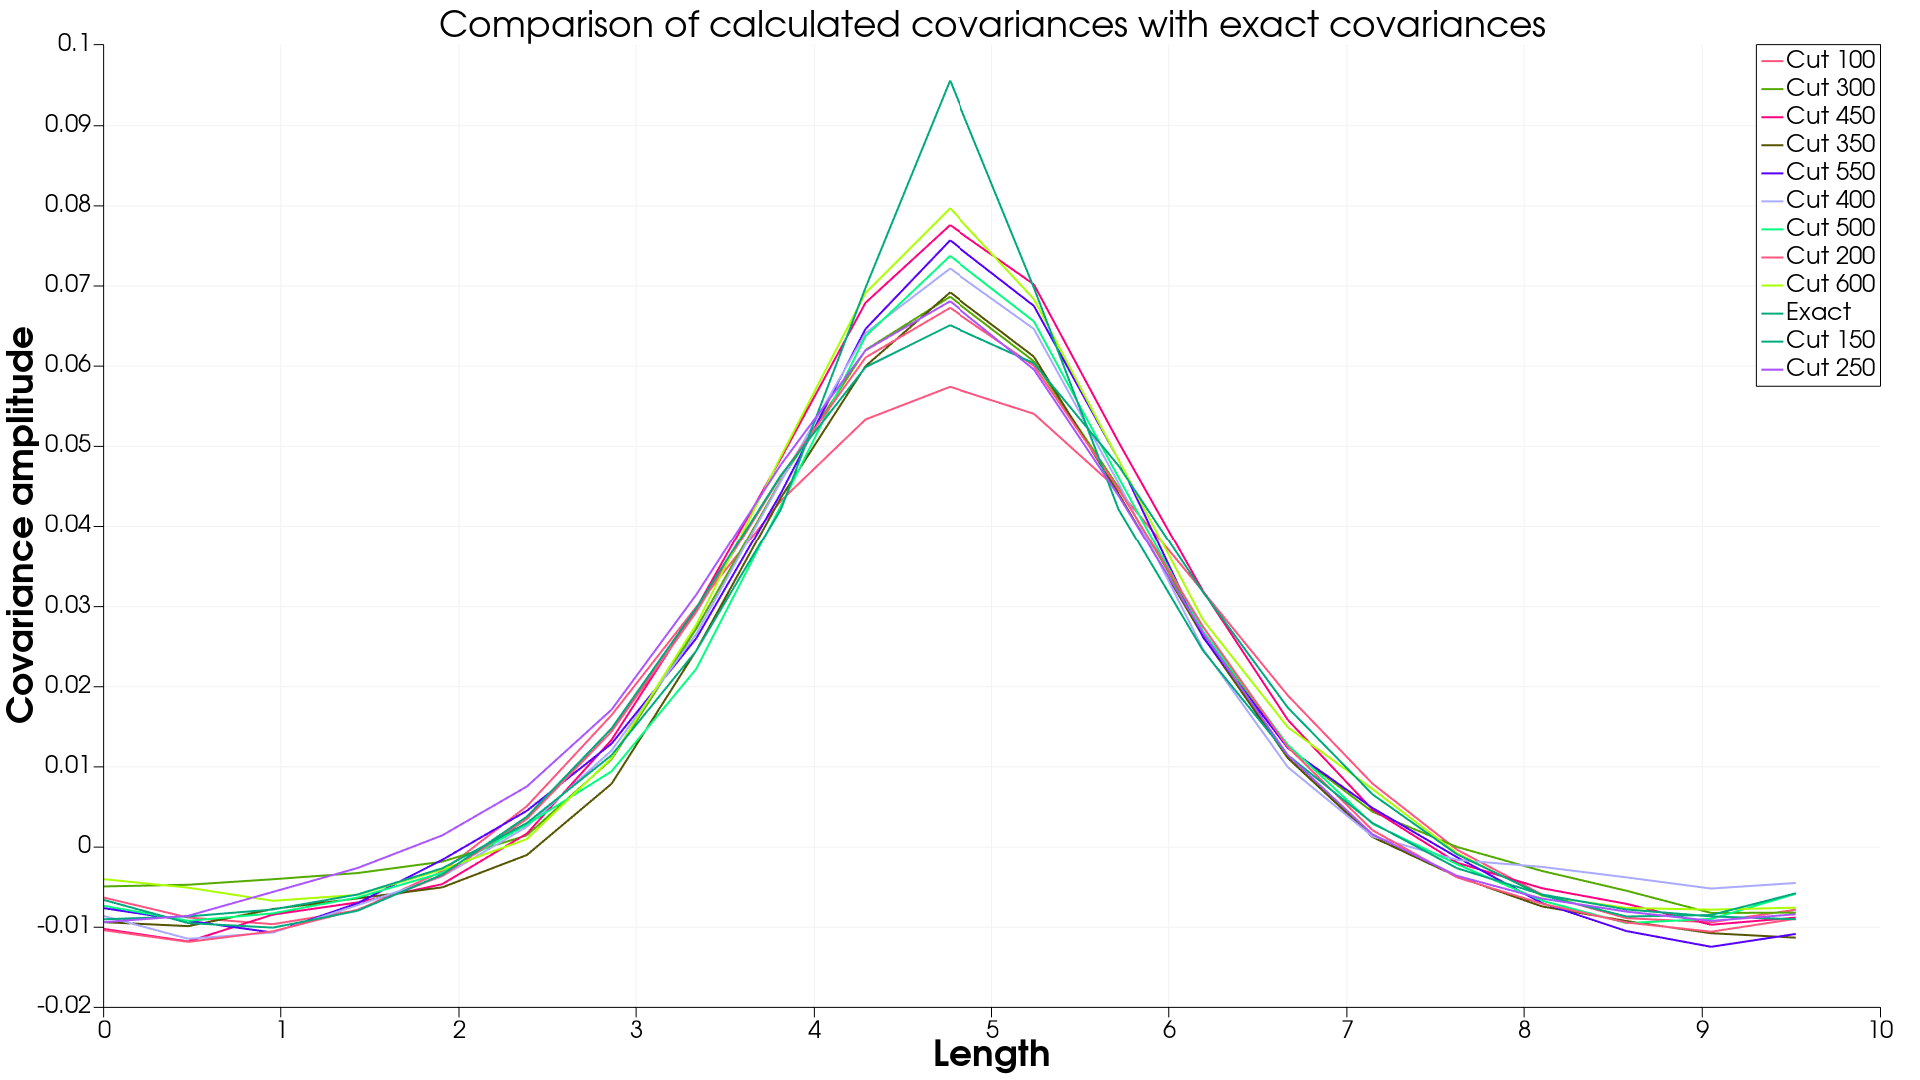
\includegraphics[width=0.45\linewidth]{comparison_covcut2_z}}
    }
    
    \onehalfspacing{Сравнение ковариацинной функции, допуск 2\%, для направлений а) вдоль диагонали, б) вдоль оси $x$, в) вдоль оси $y$, г) вдоль оси $z$}
    \caption{Сравнение ковариационной функции для допуска по амплитуде ковариаций в 2\% для различных направлений в рассматриваемой области}
    \label{img:covcut_2_comparison}  
\end{figure}
%
% Обрезание 3%
%
\begin{figure}[!ht]
    \center{
        \subcaptionbox[List-of-Figures entry]{диагональ\label{img:comparison_covcut3_diag}} 
        {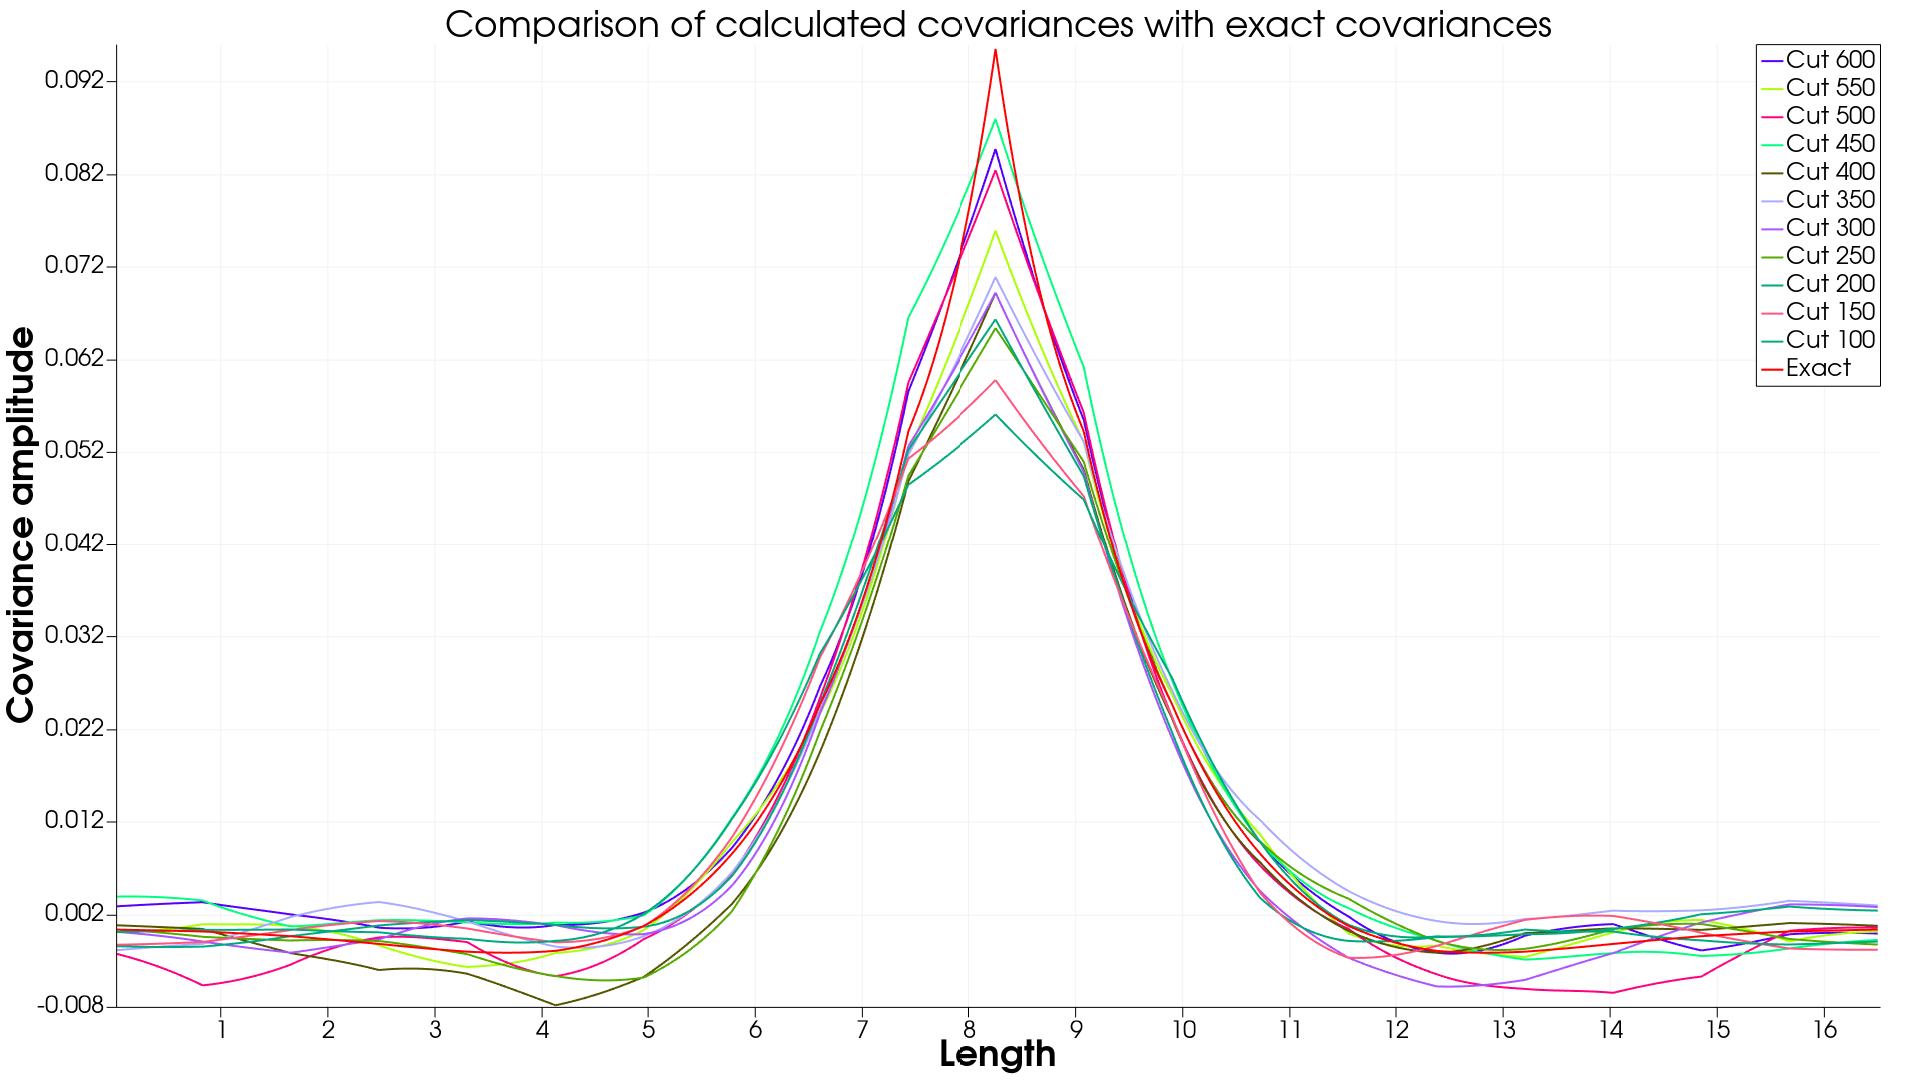
\includegraphics[width=0.45\linewidth]{comparison_covcut3_diag}}%
        \hfill
        \subcaptionbox{$x$ направление\label{img:comparison_covcut3_x}} 
        {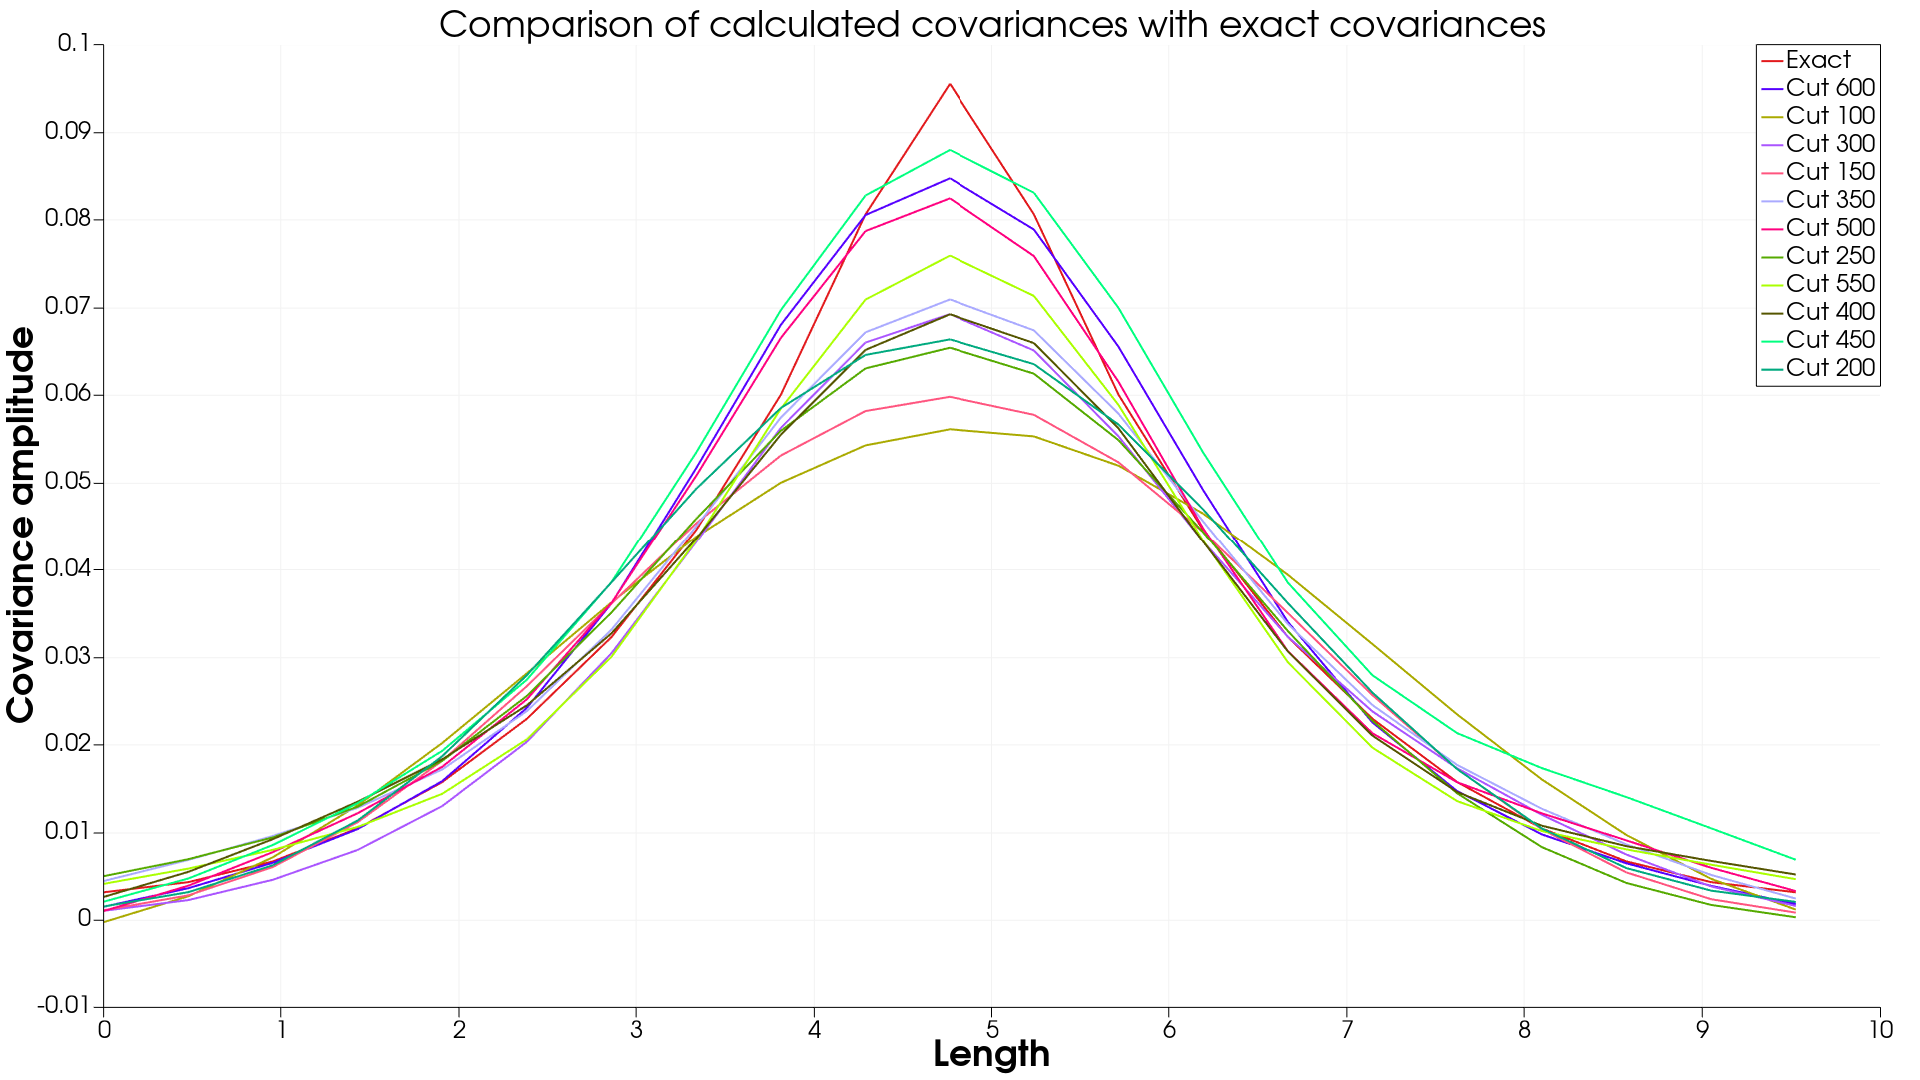
\includegraphics[width=0.45\linewidth]{comparison_covcut3_x}} \\
    }
    \center{
        \subcaptionbox[List-of-Figures entry]{$y$ направление\label{img:comparison_covcut3_y}} 
        {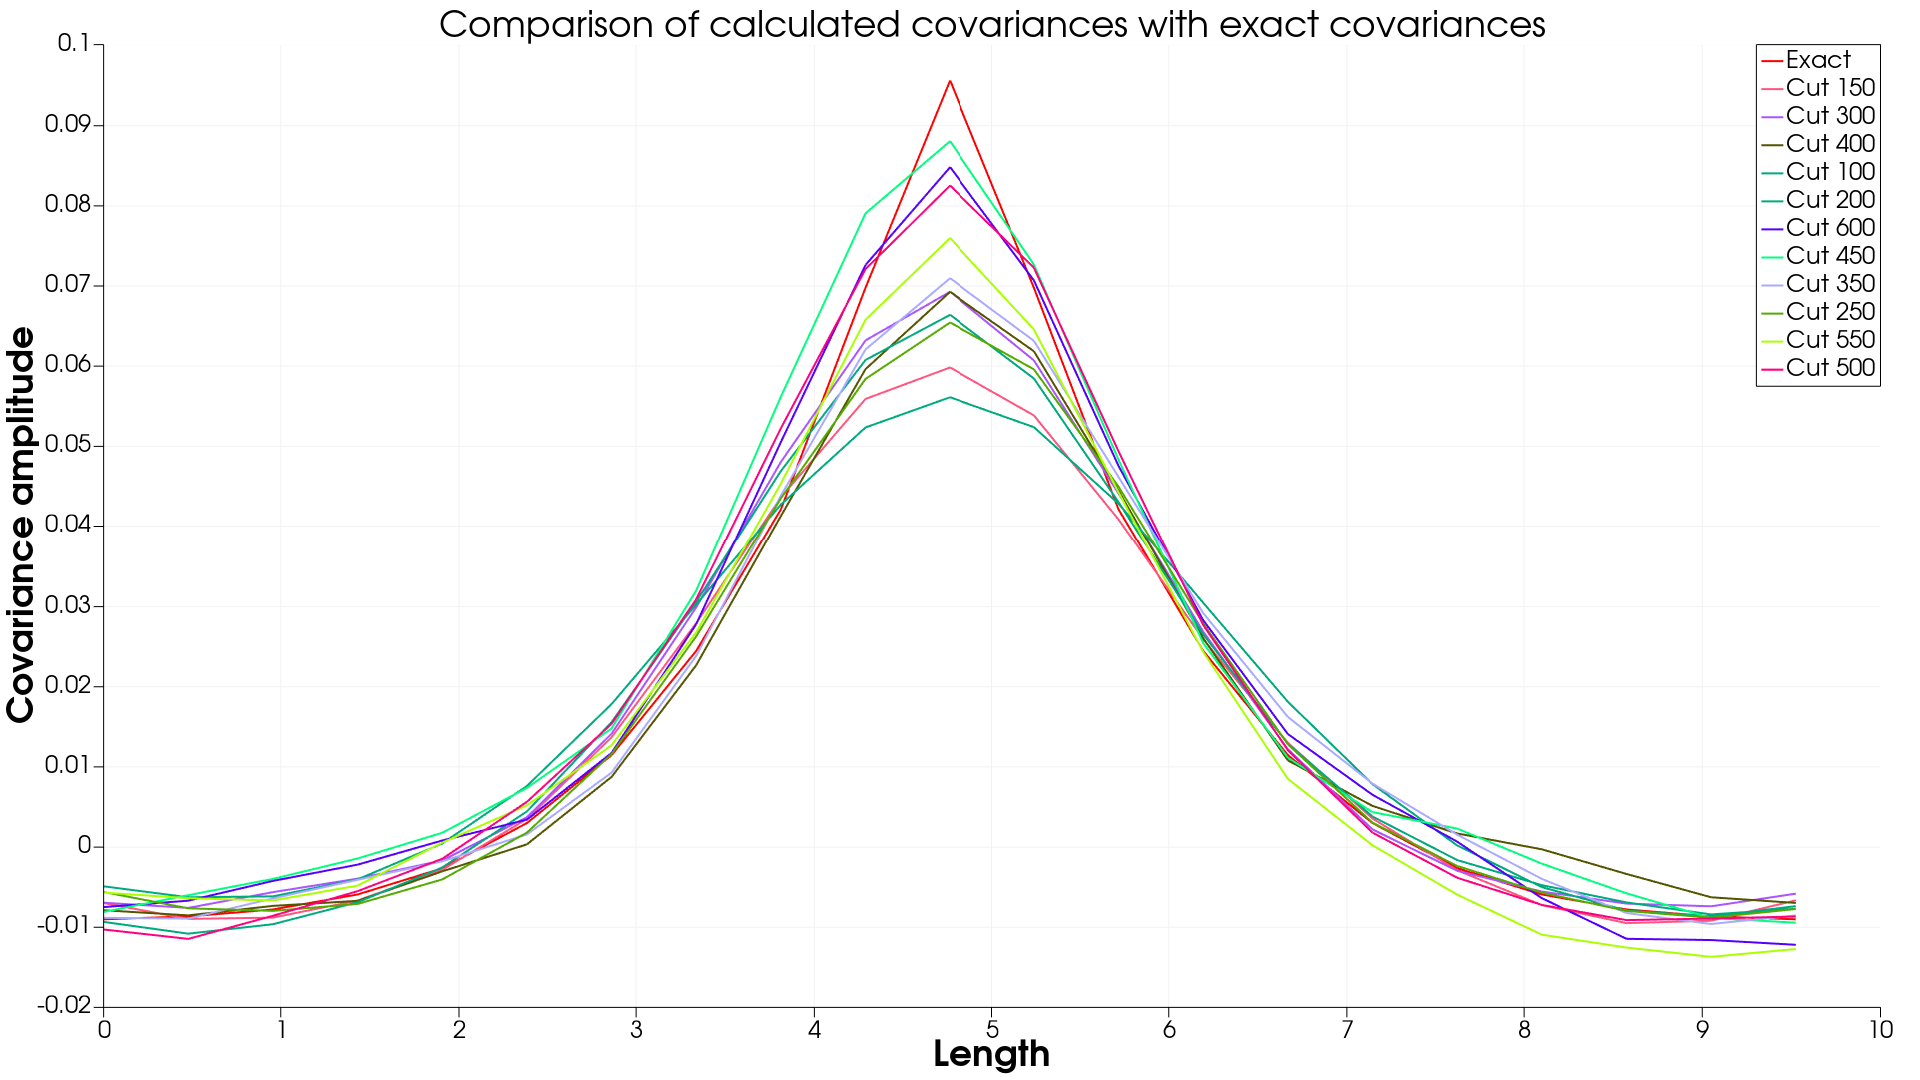
\includegraphics[width=0.45\linewidth]{comparison_covcut3_y}}%
        \hfill
        \subcaptionbox{$z$ направление\label{img:comparison_covcut3_z}} 
        {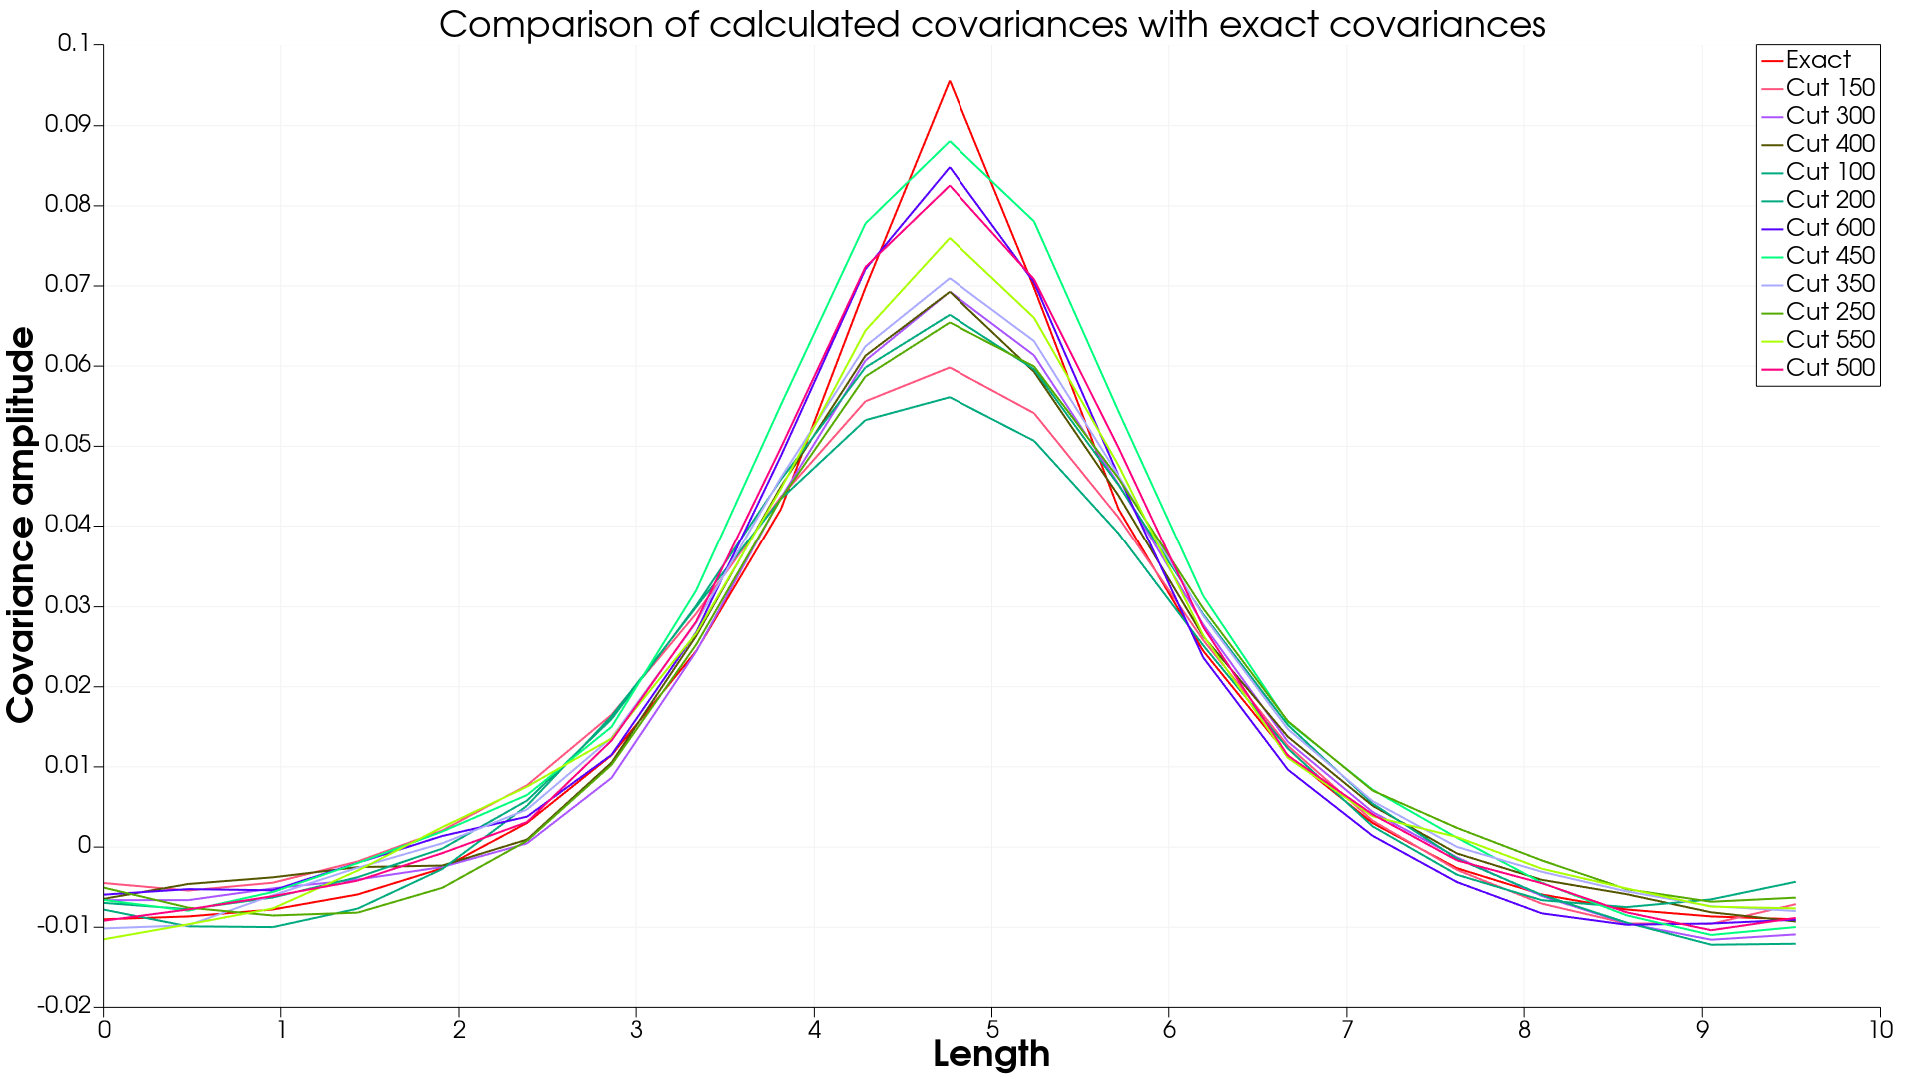
\includegraphics[width=0.45\linewidth]{comparison_covcut3_z}}

    }
    
    \onehalfspacing{Сравнение ковариацинной функции, допуск 3\%, для направлений а) вдоль диагонали, б) вдоль оси $x$, в) вдоль оси $y$, г) вдоль оси $z$}
    \caption{Сравнение ковариационной функции для допуска по амплитуде ковариаций в 3\% для различных направлений в рассматриваемой области}
    \label{img:covcut_3_comparison}  
\end{figure}
%
% Обрезание 4%
%
\begin{figure}[!ht]
    \center{

        \subcaptionbox[List-of-Figures entry]{диагональ\label{img:comparison_covcut4_diag}} 
        {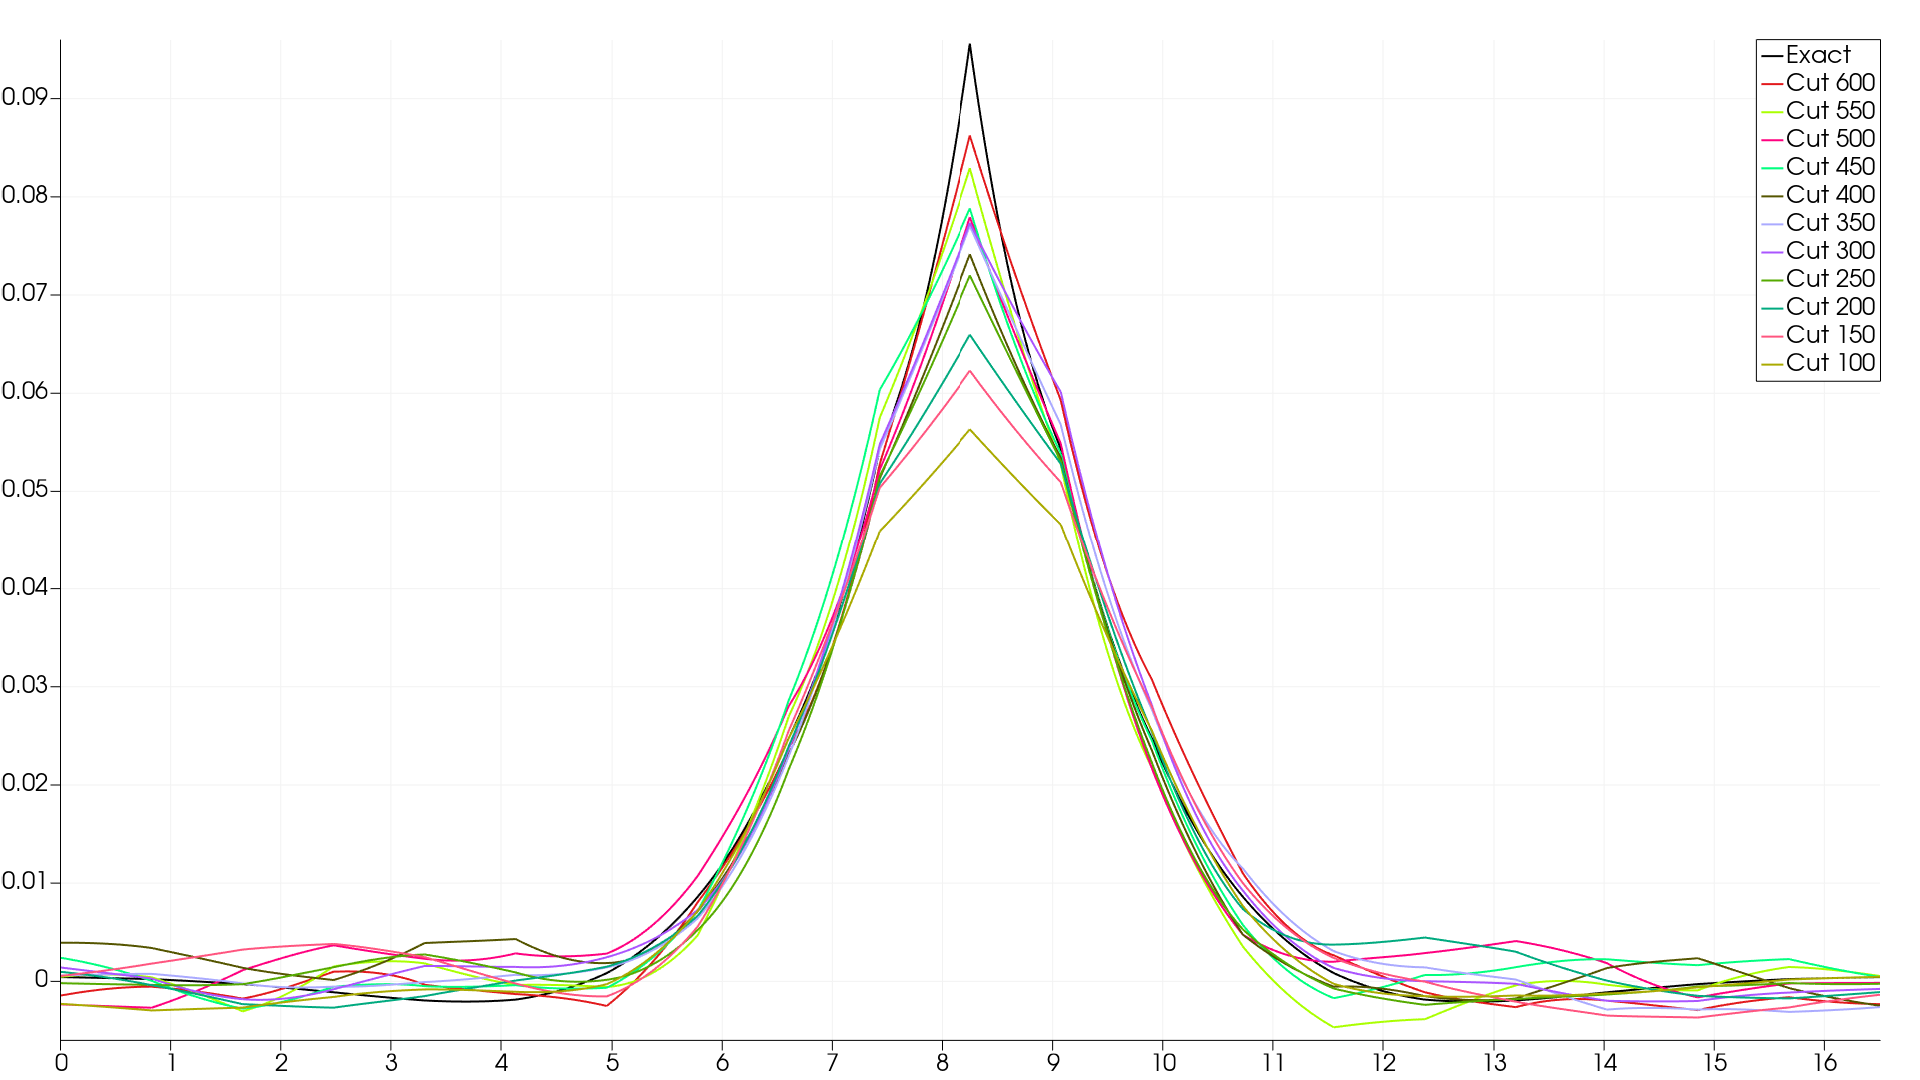
\includegraphics[width=0.45\linewidth]{comparison_covcut4_diag}}%
        \hfill
        \subcaptionbox{$x$ направление\label{img:comparison_covcut4_x}} 
        {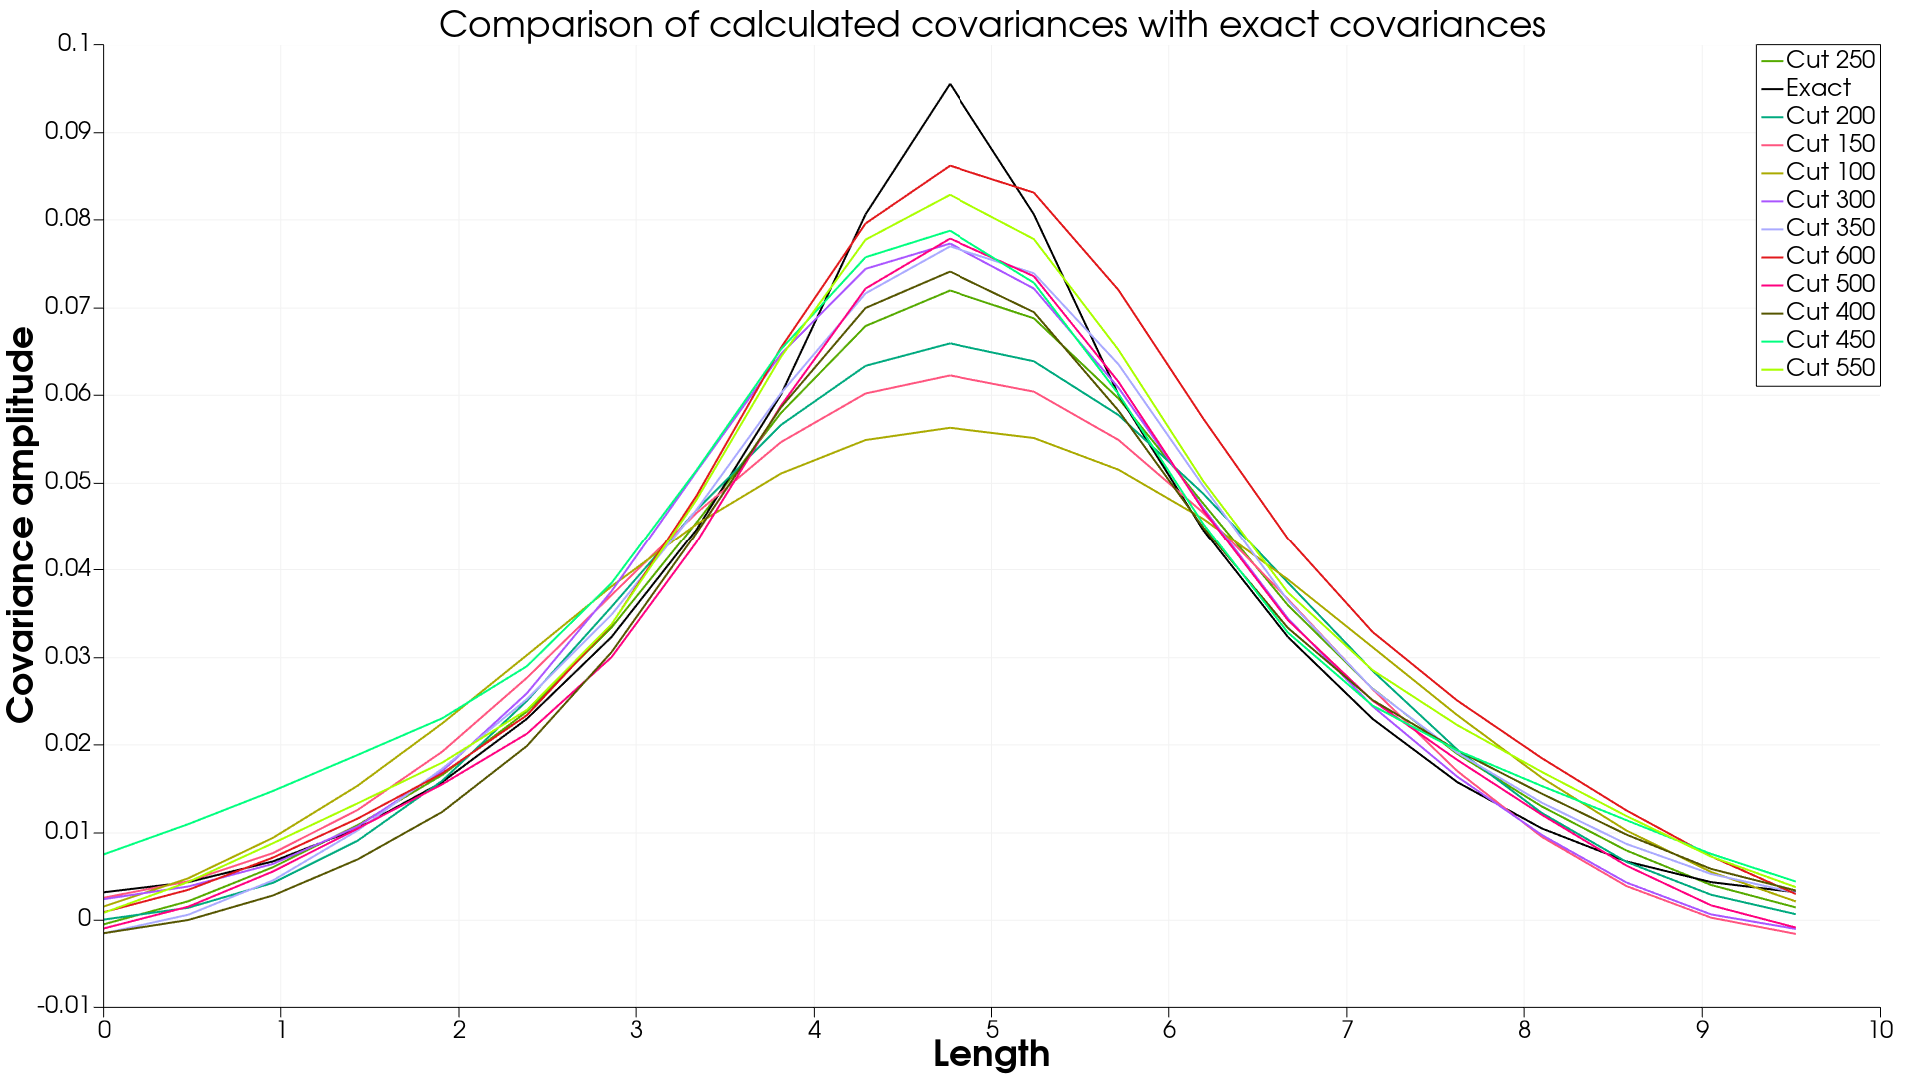
\includegraphics[width=0.45\linewidth]{comparison_covcut4_x}} \\
    }
    \center{
        \subcaptionbox[List-of-Figures entry]{$y$ направление\label{img:comparison_covcut4_y}} 
        {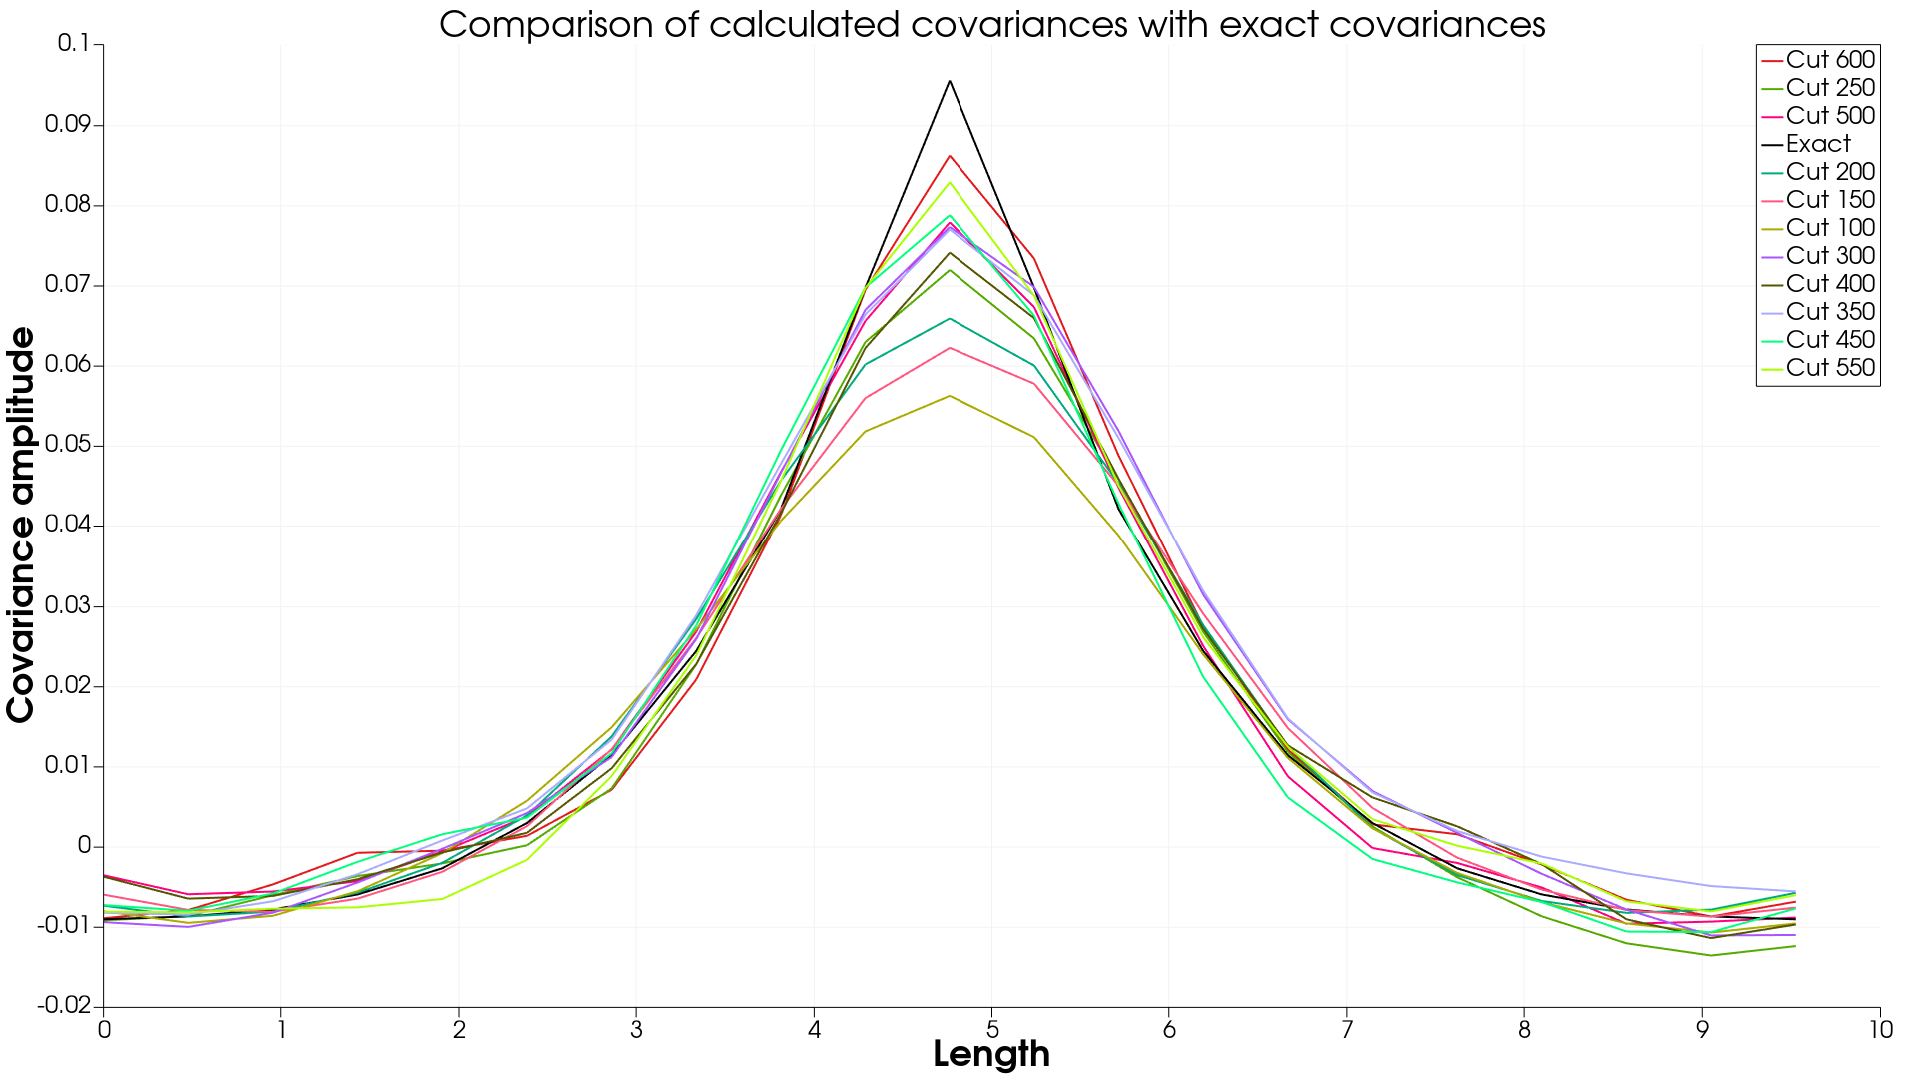
\includegraphics[width=0.45\linewidth]{comparison_covcut4_y}}%
        \hfill
        \subcaptionbox{$z$ направление\label{img:comparison_covcut4_z}} 
        {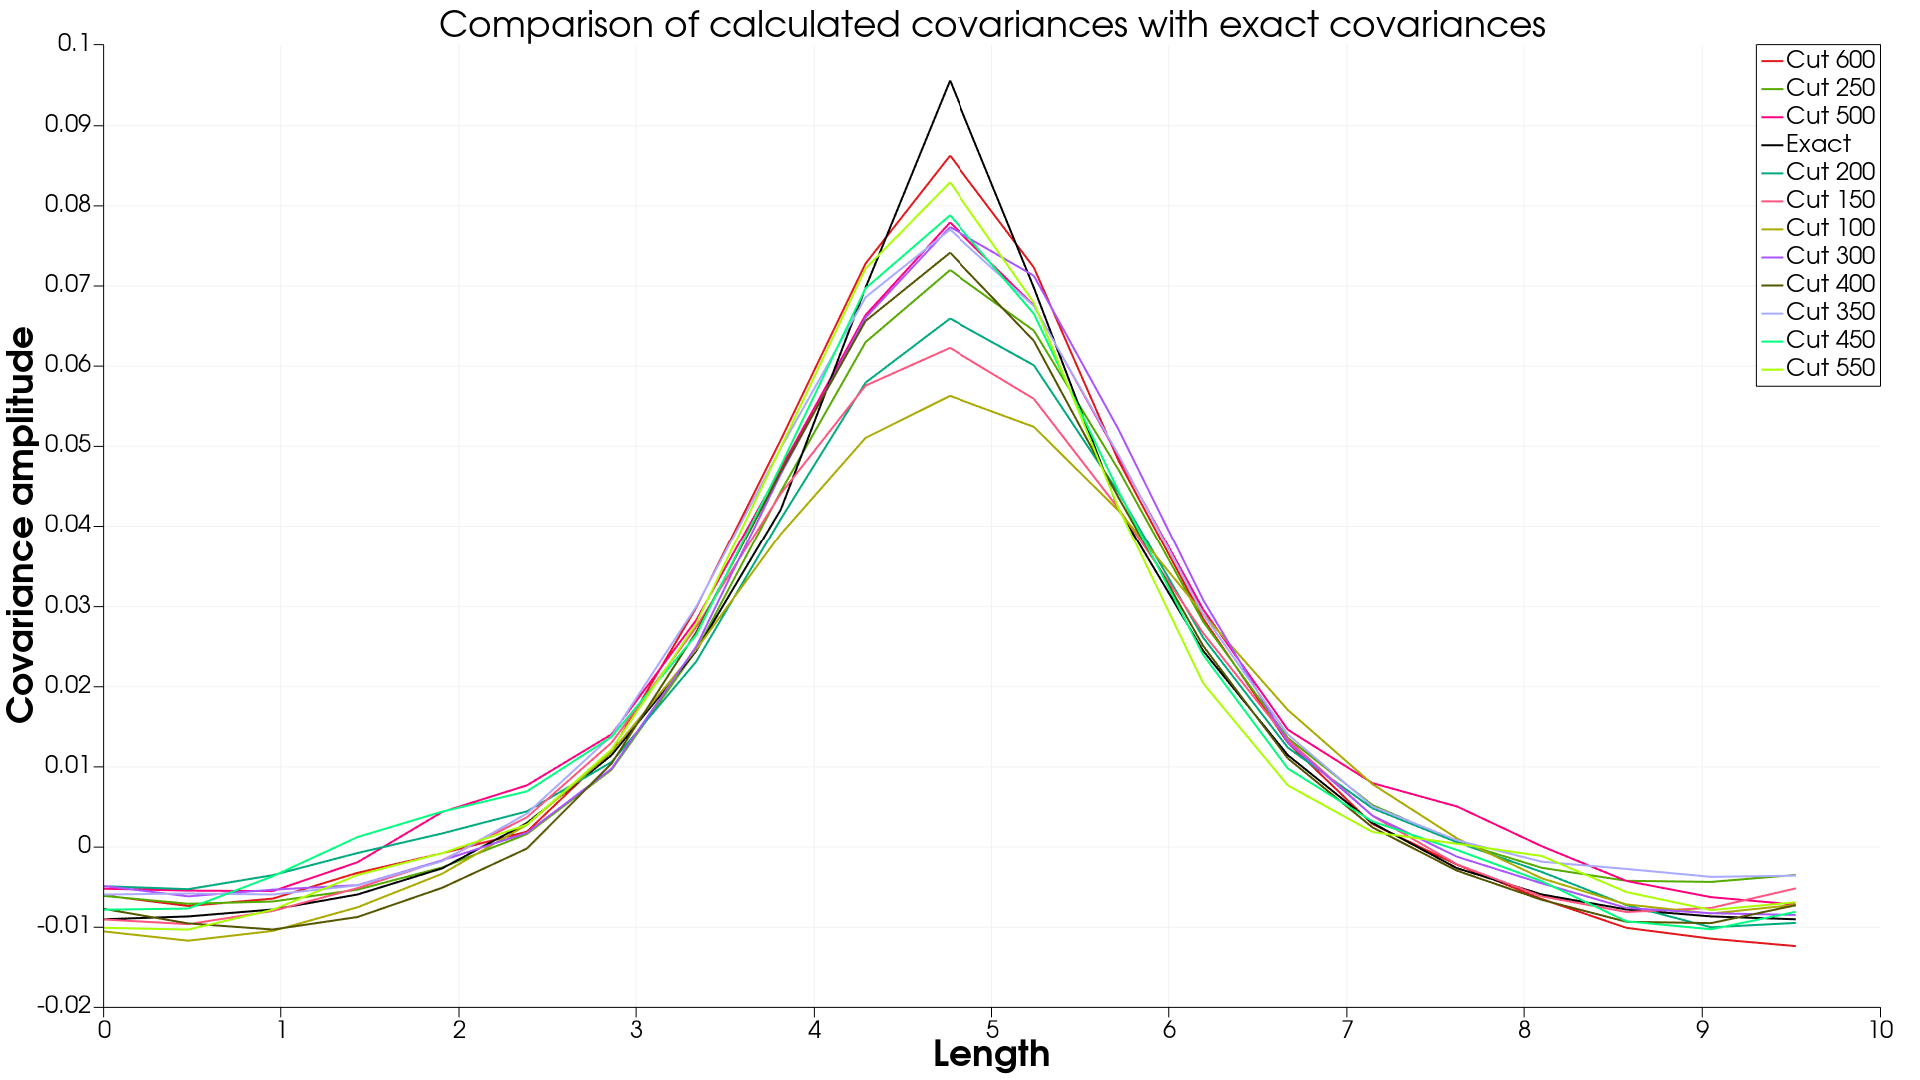
\includegraphics[width=0.45\linewidth]{comparison_covcut4_z}}

    }
    
    \onehalfspacing{Сравнение ковариацинной функции, допуск 4\%, для направлений а) вдоль диагонали, б) вдоль оси $x$, в) вдоль оси $y$, г) вдоль оси $z$}
    \caption{Сравнение ковариационной функции для допуска по амплитуде ковариаций в 4\% для различных направлений в рассматриваемой области}
    \label{img:covcut_4_comparison}  
\end{figure}
%
% Обрезание 5%
%
\begin{figure}[!ht]
    \center{

        \subcaptionbox[List-of-Figures entry]{диагональ\label{img:comparison_covcut5_diag}} 
        {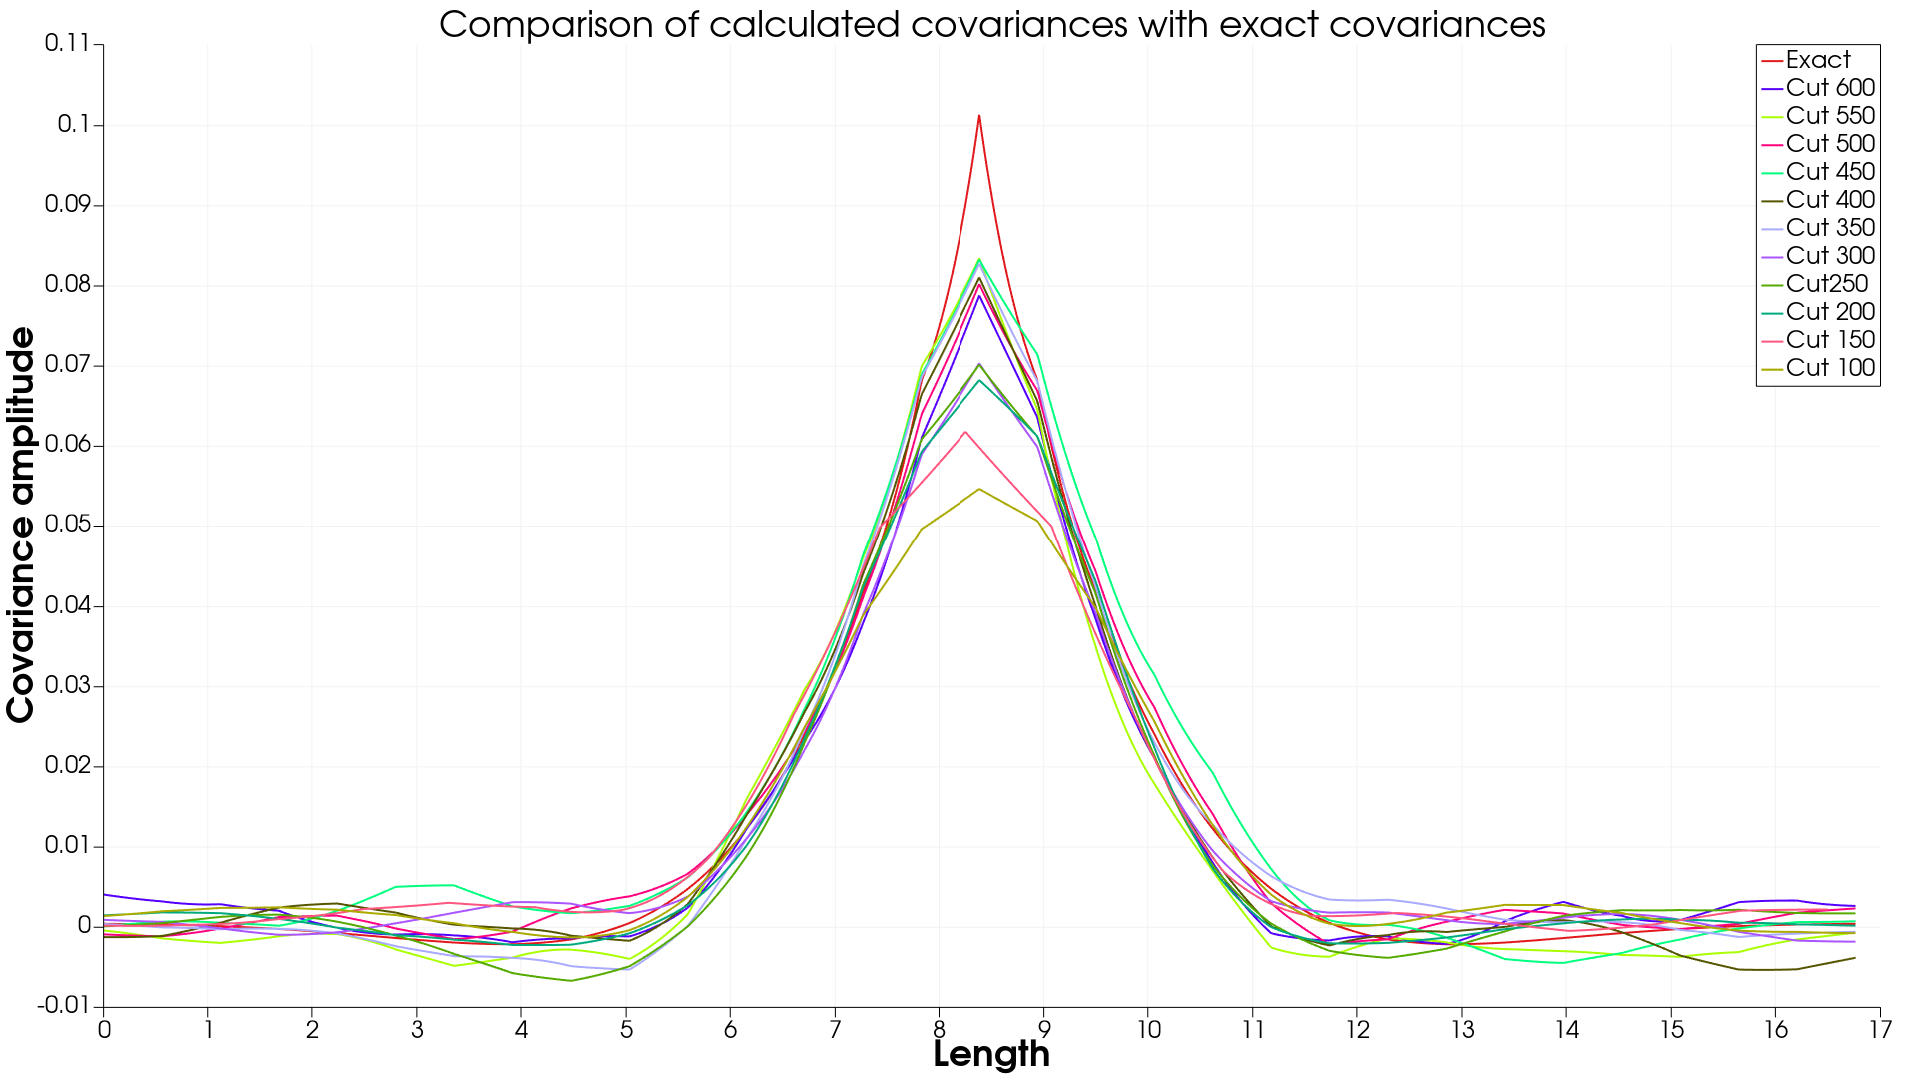
\includegraphics[width=0.45\linewidth]{comparison_covcut5_diag}}%
        \hfill
        \subcaptionbox{$x$ направление\label{img:comparison_covcut5_x}} 
        {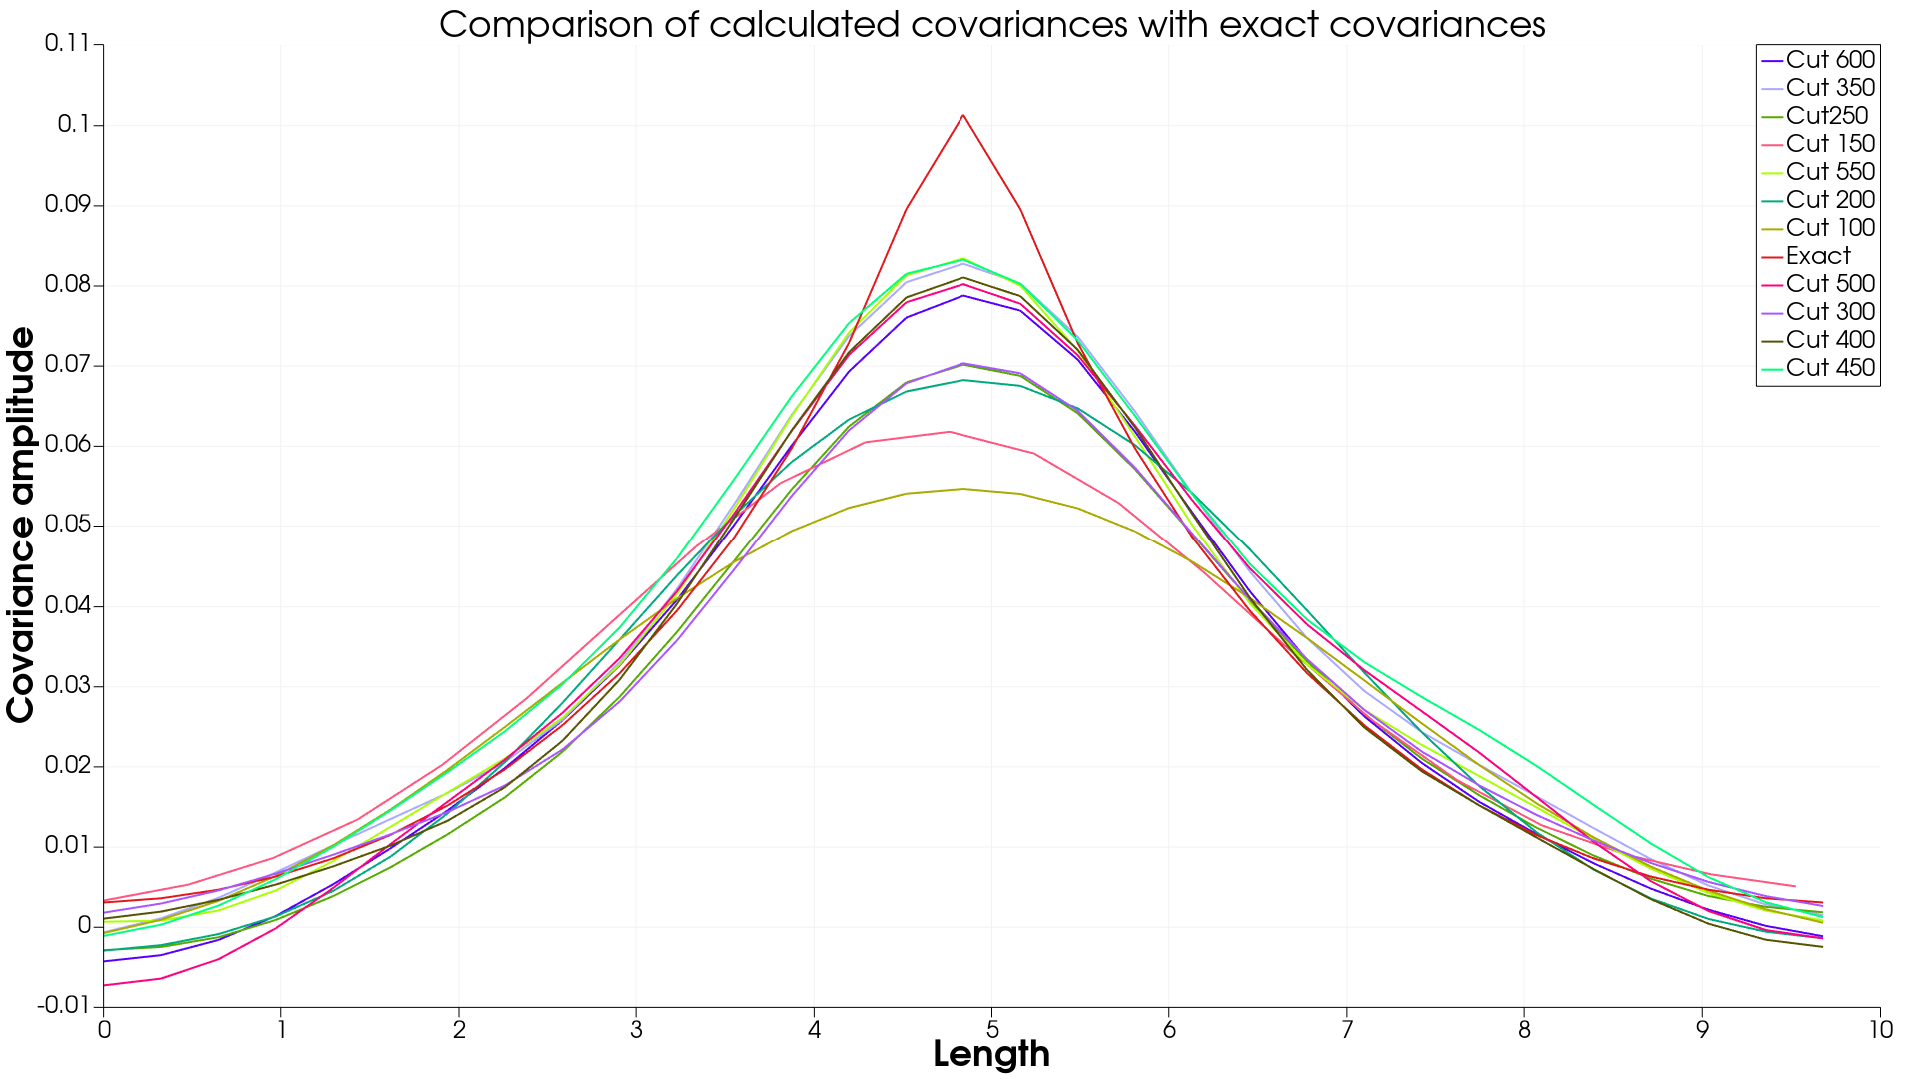
\includegraphics[width=0.45\linewidth]{comparison_covcut5_x}} \\
    }
    \center{
        \subcaptionbox[List-of-Figures entry]{$y$ направление\label{img:comparison_covcut5_y}} 
        {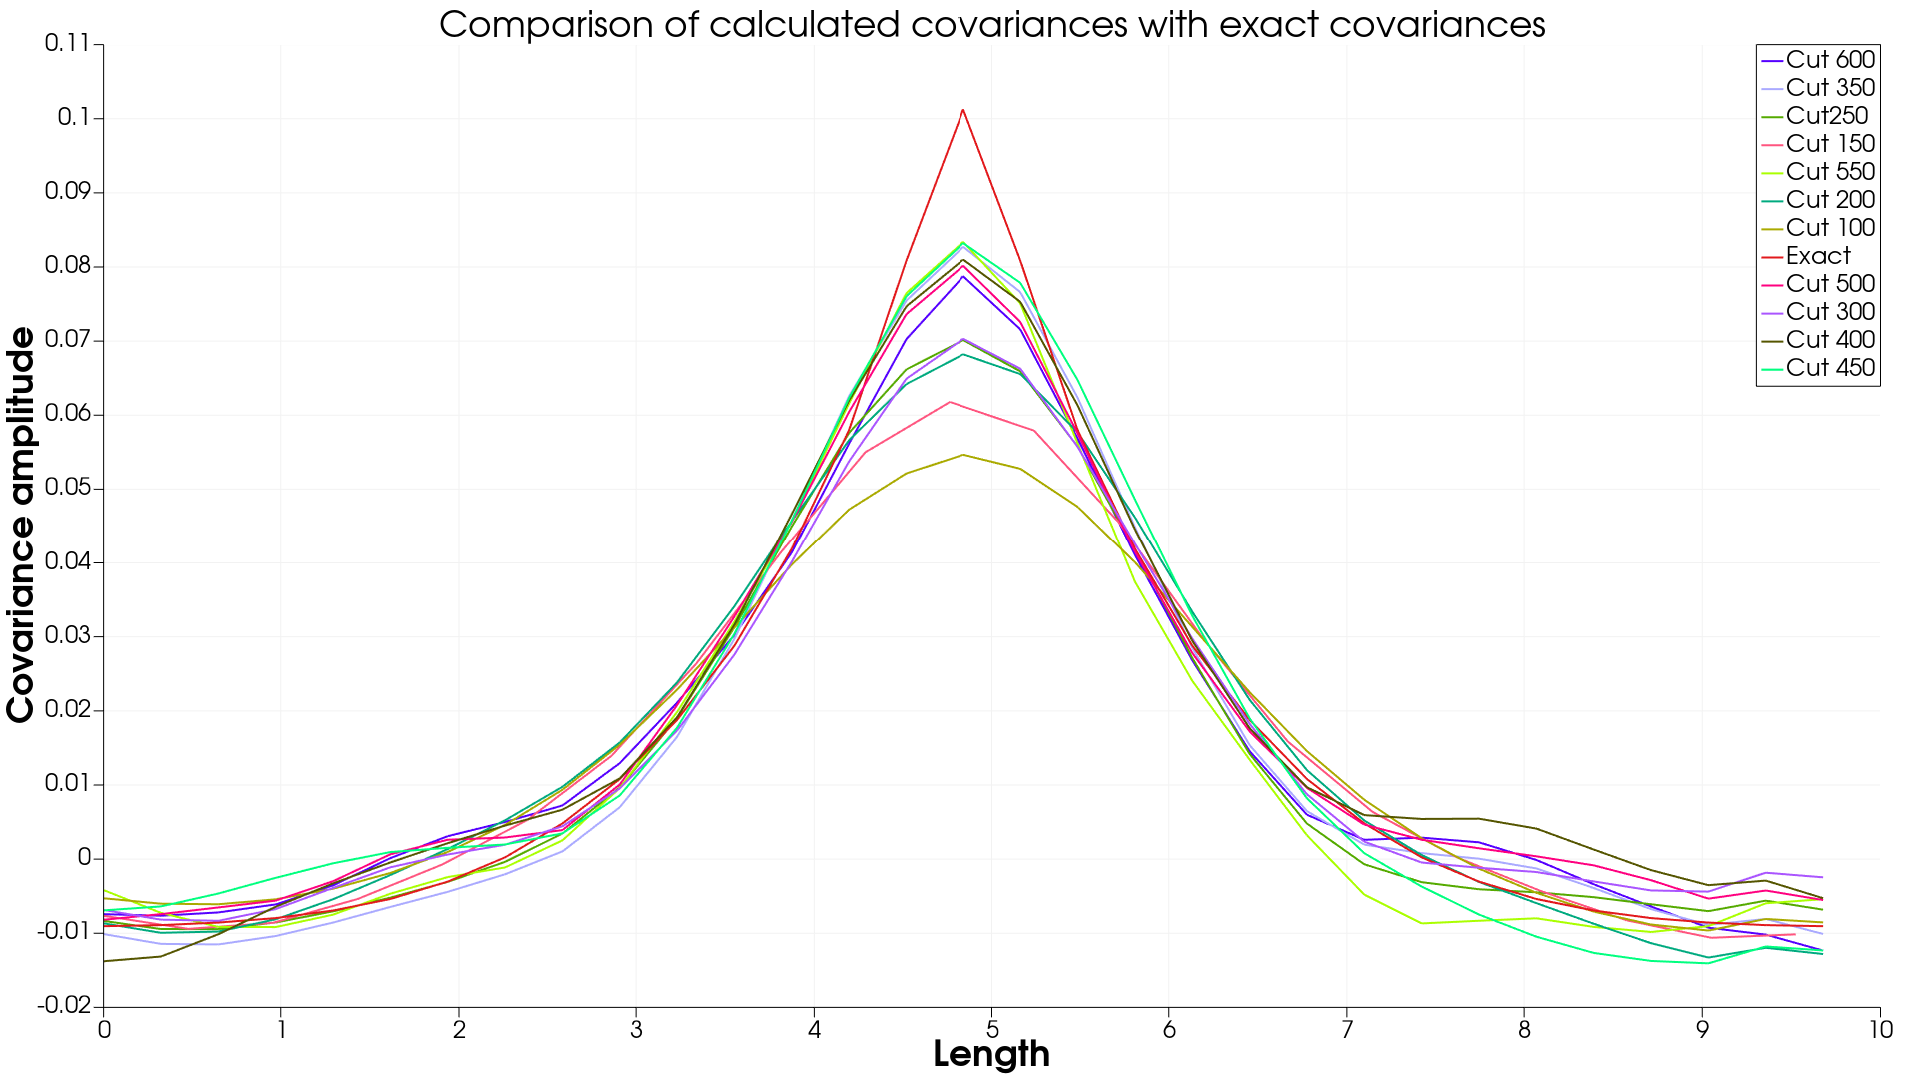
\includegraphics[width=0.45\linewidth]{comparison_covcut5_y}}%
        \hfill
        \subcaptionbox{$z$ направление\label{img:comparison_covcut5_z}} 
        {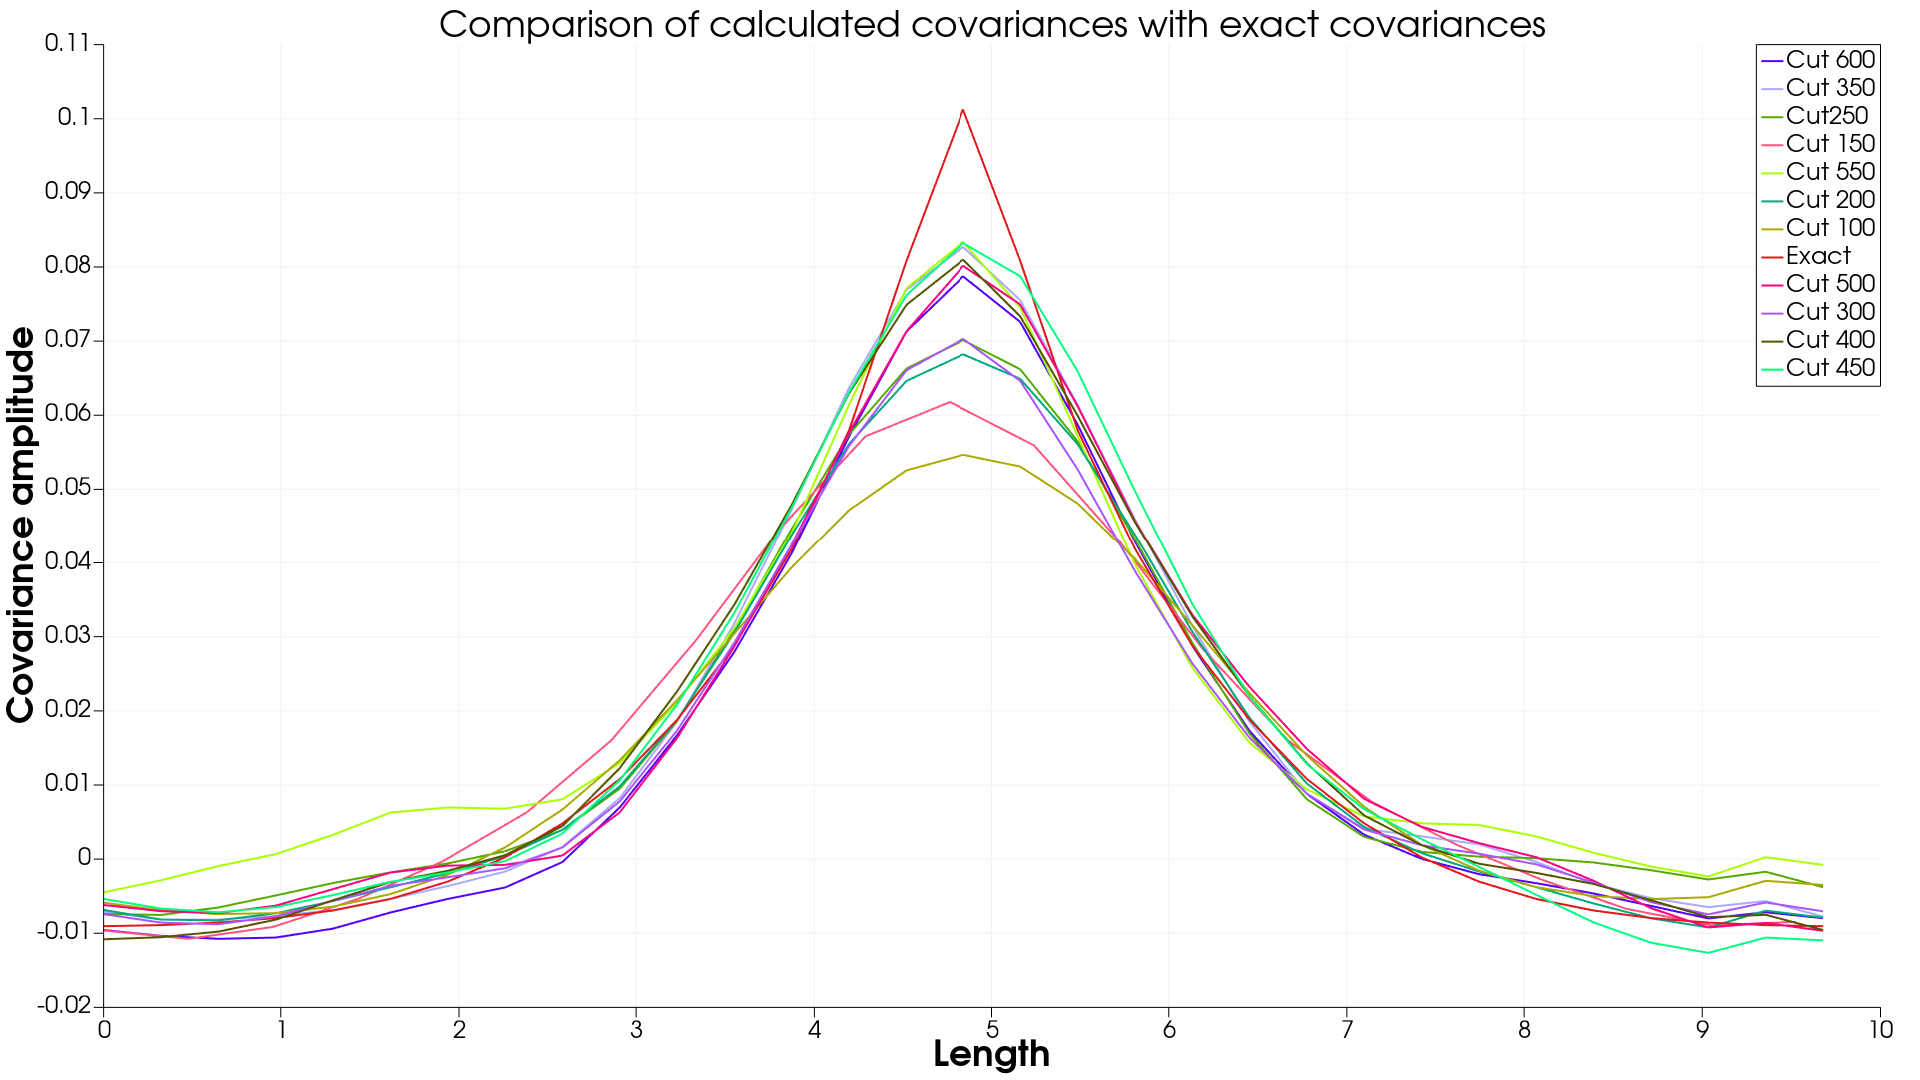
\includegraphics[width=0.45\linewidth]{comparison_covcut5_z}}

    }
    
    \onehalfspacing{Сравнение ковариацинной функции, допуск 5\%, для направлений а) вдоль диагонали, б) вдоль оси $x$, в) вдоль оси $y$, г) вдоль оси $z$}
    \caption{Сравнение ковариационной функции для допуска по амплитуде ковариаций в 5\% для различных направлений в рассматриваемой области}
    \label{img:covcut_5_comparison}  
\end{figure}

Так как расчёт статистических параметров, например ковариационной функции, требует какого-то набора реализаций полей скорости, необходимо также проверить, как влияет число генерируемых полей для подсчёта статистических характеристик. Это важный критерий в силу того, что основными параметрами валидации являются статистические величины. Естественно, наиболее точный случай это бесконечное число реализаций, но это также несёт в себе дополнительные временные затраты. Например, если необходимо для случая генерации поля на некоторой сетке оценить то, как хорошо метод подходит для использования на данной топологии сетки, или, например, какое число собственных значений и векторов стоит брать для последующей генерации флуктуации необходимо провести статистическое исследование, дабы не увеличивать требуемое время, стоит провести оценку некоторого оптимального числа реализаций, на котором можно проводить последующие валидации. На рисунке \ref{covcut0_eigvalues_step_samples} ниже представлены сравнение ковариационных функций, полученных в результате использования $n$ реализаций поля скоростей для подсчёта. В целом, для числа реализаций равного 1000, уже наблюдается хорошее совпадение с целевым спектром вблизи его пика, чем дальше мы отдаляемся от центра куба, тем сильнее начинает играть роль число взятых сгенерированных полей. С ростом числа взятых для расчёта реализаций также уменьшается разница между целевой ковариационной функций и рассчитанной.

\begin{figure}[!ht]
    \center{

        \subcaptionbox[List-of-Figures entry]{диагональ\label{img:diagonal_alleigenvalues_samples_step}} 
        {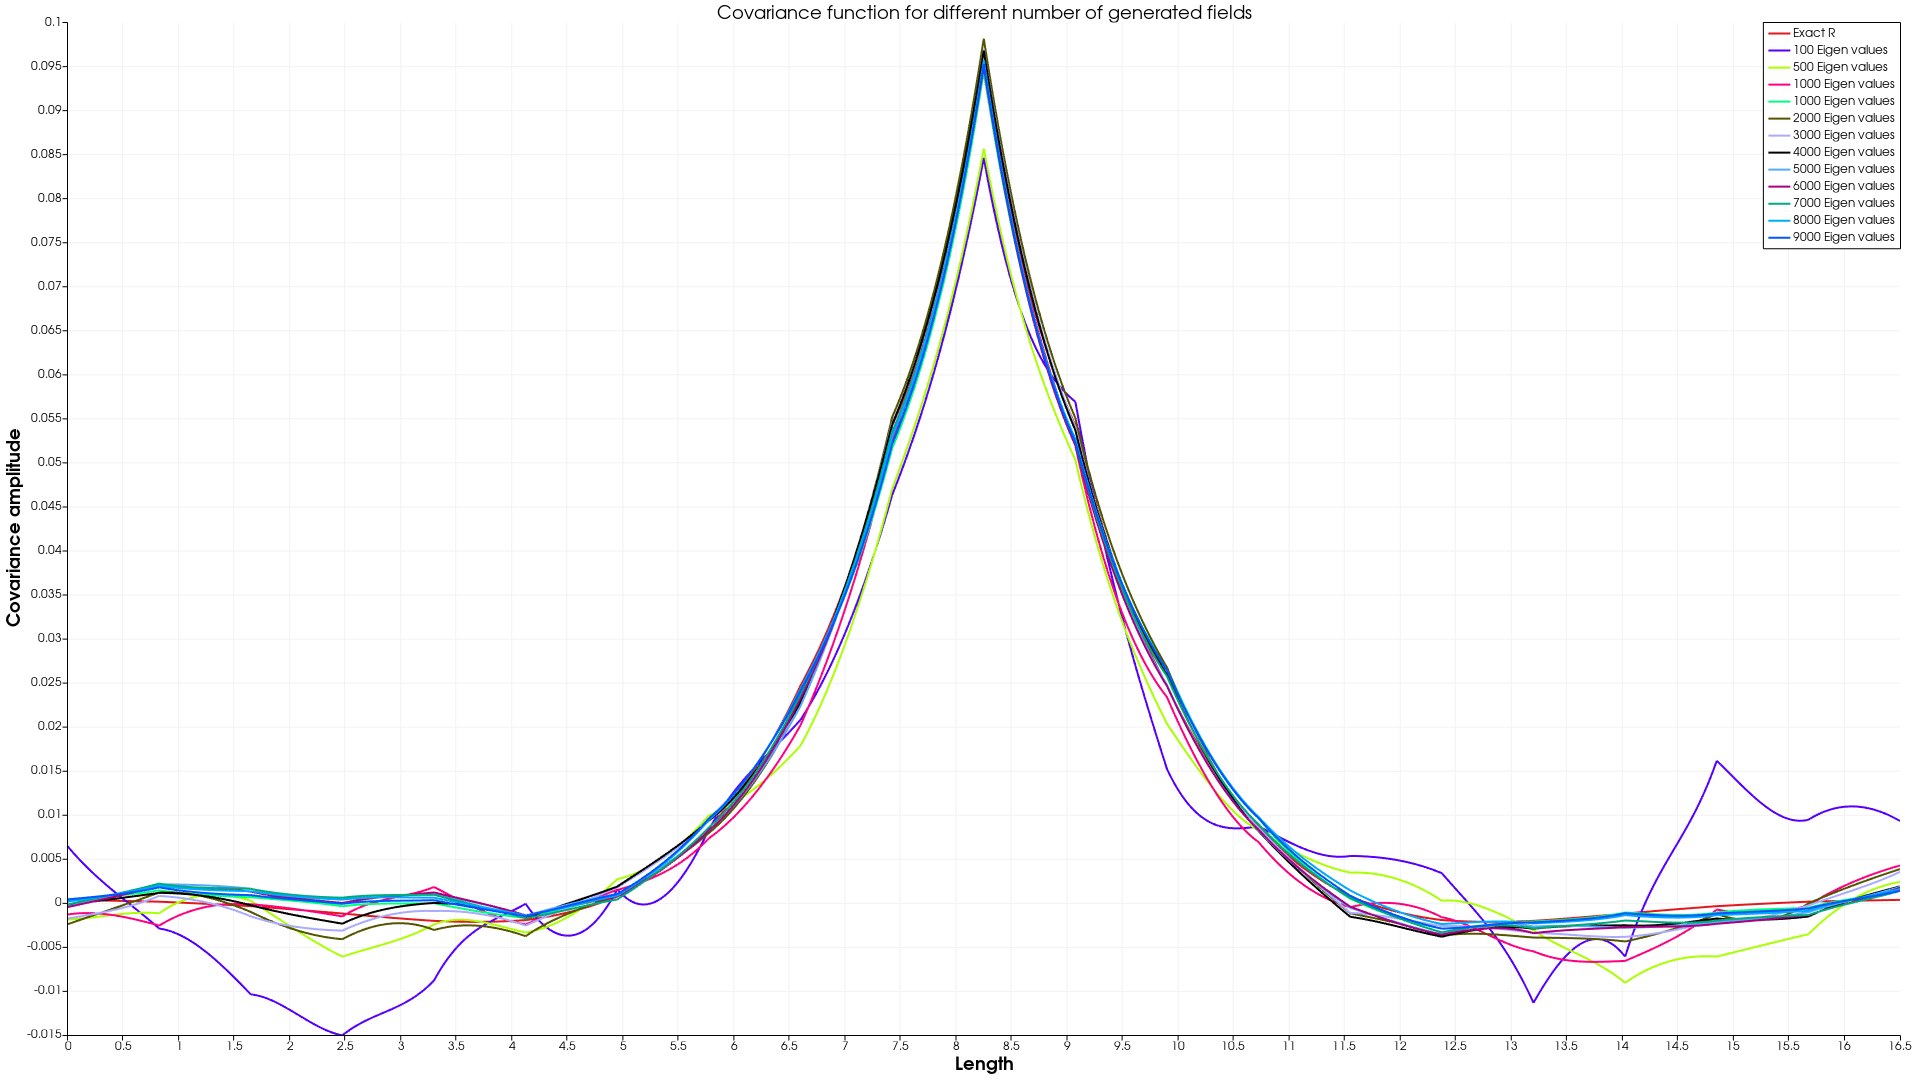
\includegraphics[width=0.45\linewidth]{diagonal_alleigenvalues_samples_step}}%
        \hfill
        \subcaptionbox{$x$ направление\label{img:x_axis_alleigenvalues_samples_step}} 
        {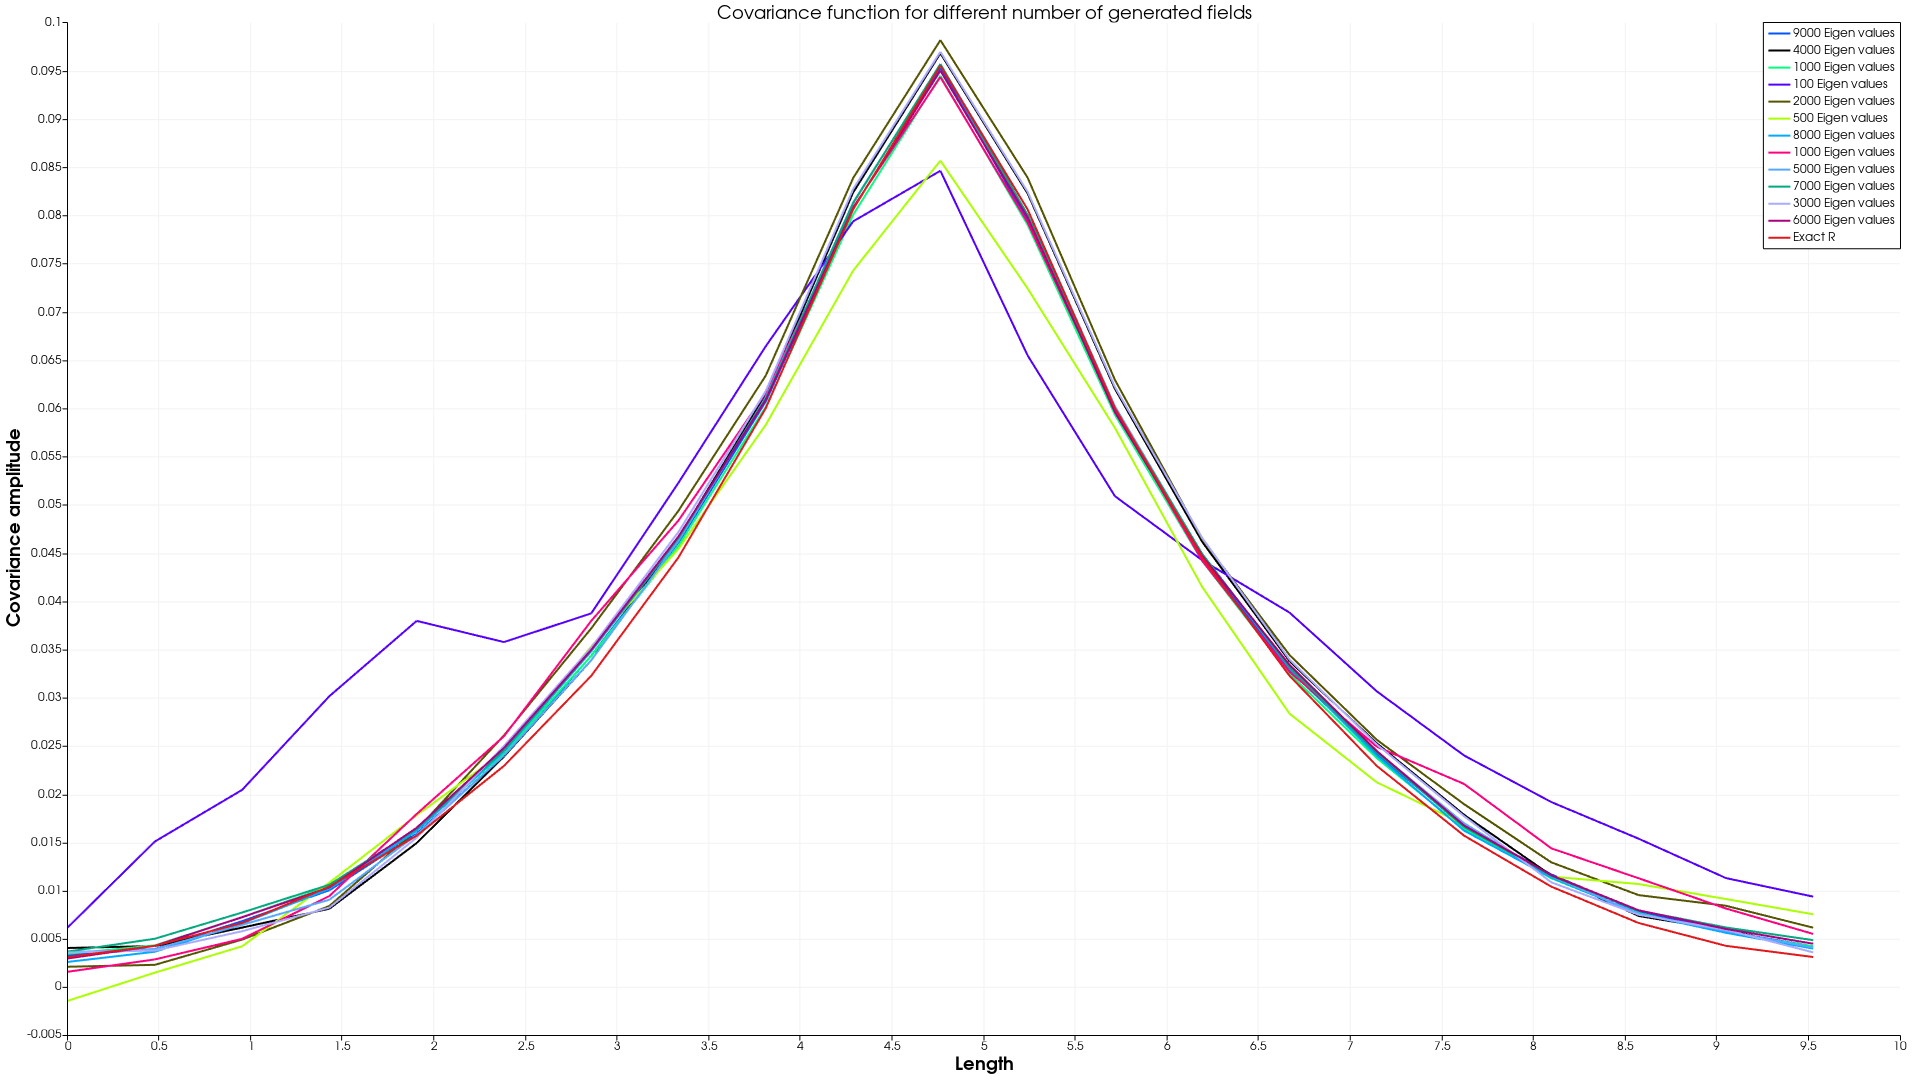
\includegraphics[width=0.45\linewidth]{x_axis_alleigenvalues_samples_step}} \\
    }
    \center{
        \subcaptionbox[List-of-Figures entry]{$y$ направление\label{img:y_axis_alleigenvalues_samples_step}} 
        {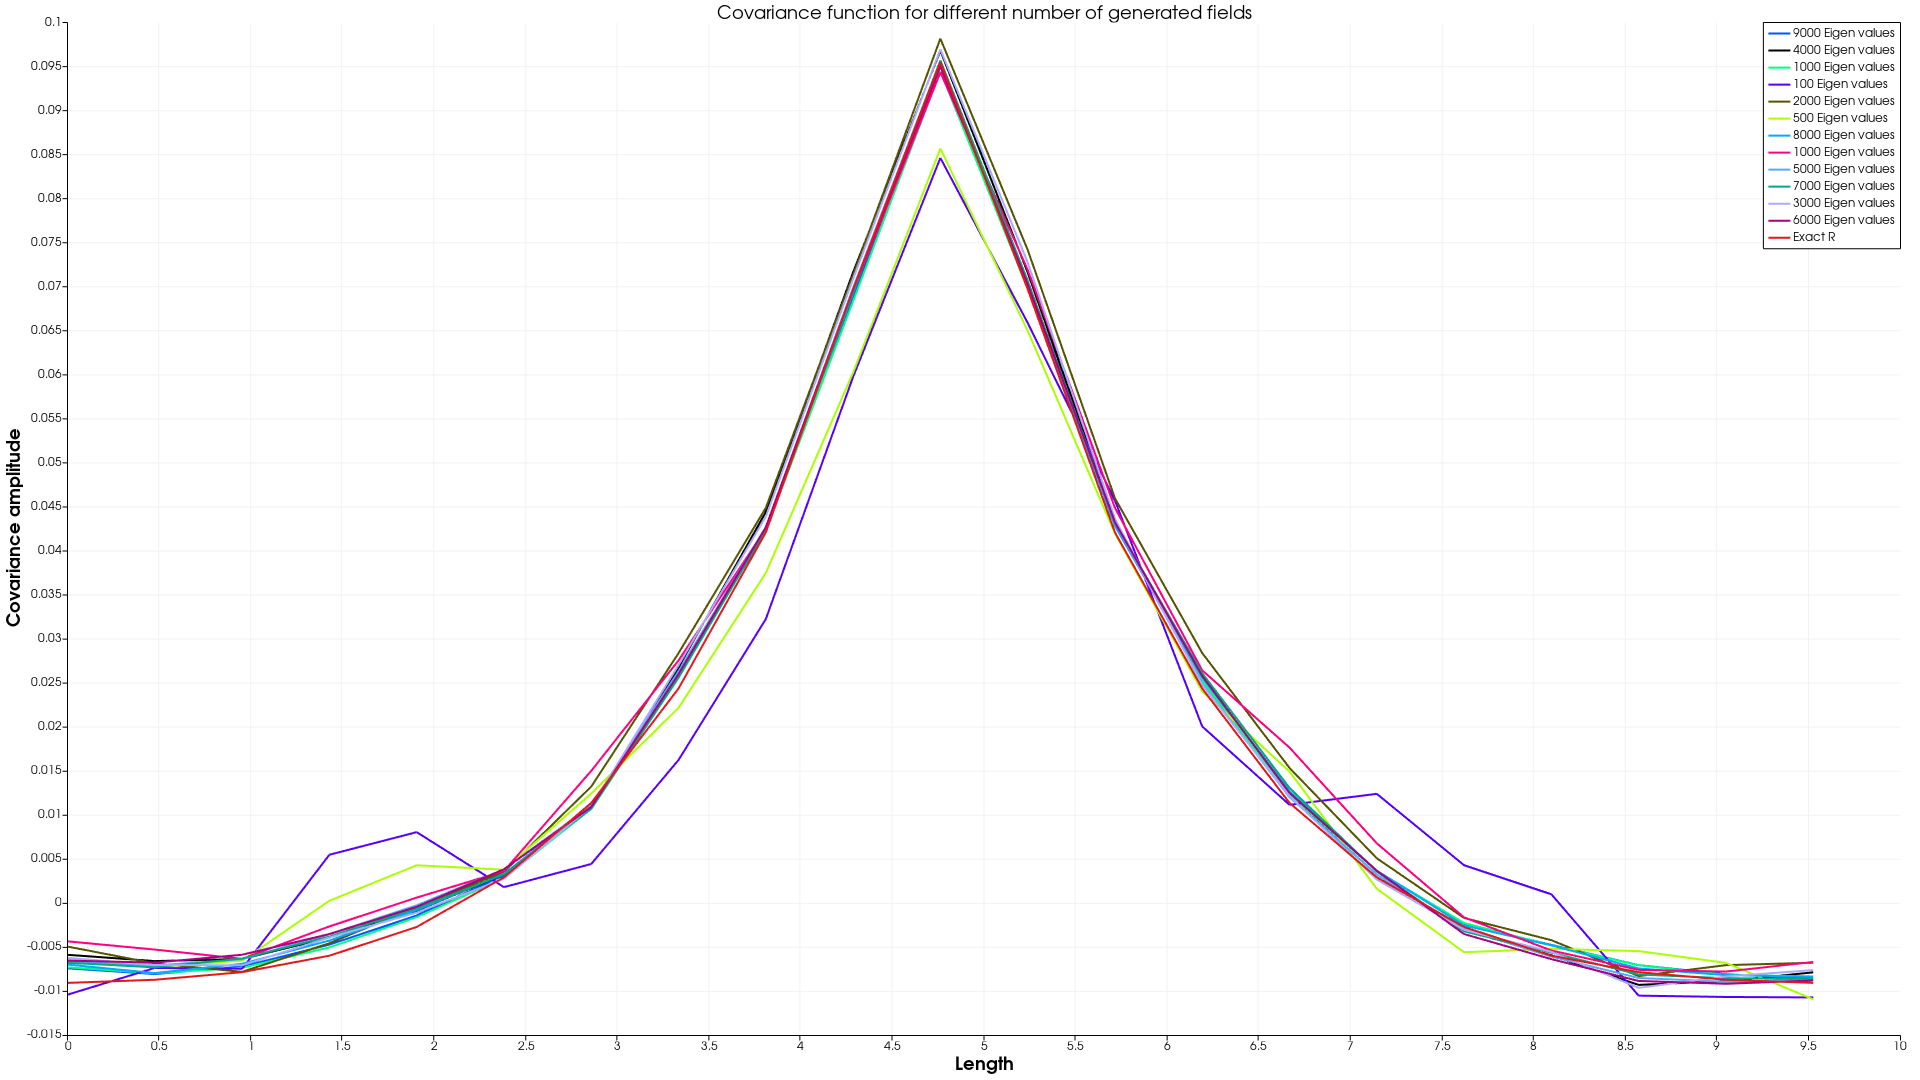
\includegraphics[width=0.45\linewidth]{y_axis_alleigenvalues_samples_step}}%
        \hfill
        \subcaptionbox{$z$ направление\label{img:z_axis_alleigenvalues_samples_step}} 
        {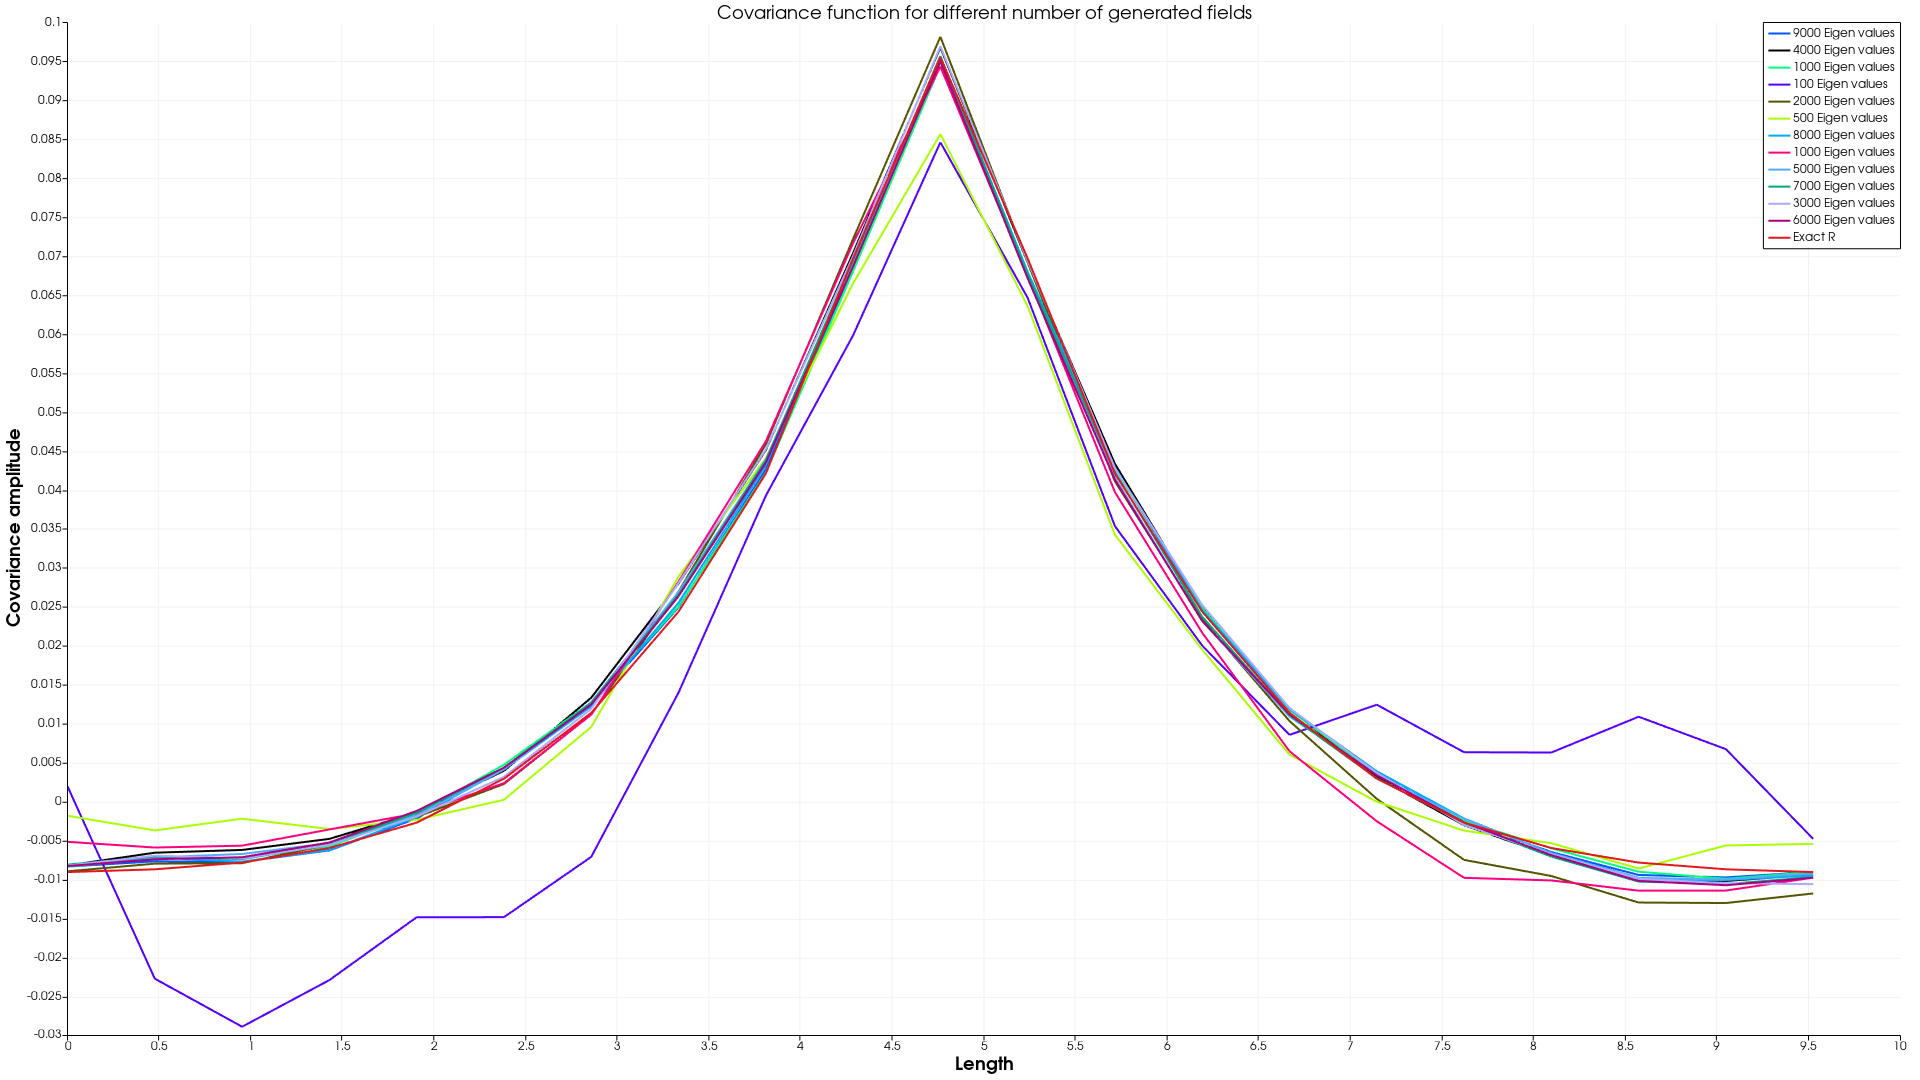
\includegraphics[width=0.45\linewidth]{z_axis_alleigenvalues_samples_step}}
    }
    
    \onehalfspacing{Сравнение ковариацинной функции, допуск 0\%, для направлений а) вдоль диагонали, б) вдоль оси $x$, в) вдоль оси $y$, г) вдоль оси $z$}
    \caption{Сравнение ковариационной функции для допуска по амплитуде ковариаций в 0\% для различного числа взятых реализаций полей флуктуаций для расчёта ковариационной функции в рассматриваемой области}
    \label{img:covcut0_eigvalues_step_samples}  
\end{figure}

\begin{table} [!h]%
	\caption{Величина разности между пиками для смоделированных ковариационных функций с пиком полученным из аналитического спектра преобразованием Фурье}%
	\label{tbl:peak_diff_table}
    \setlength\extrarowheight{4pt} %вот этим управляем расстоянием между рядами, \arraystretch даёт неудачный результат
    \setlength{\tymin}{1.5cm}
\begin{tabulary}{\textwidth}{@{}>{\zz}L >{\zz}C >{\zz}C >{\zz}C >{\zz}C >{\zz}C >{\zz}C@{}}
        \toprule     %%% верхняя линейка
            Число собственных значений &
            Допуск 0\% &
            Допуск 1\% &
            Допуск 2\% &
            Допуск 3\% &
            Допуск 4\% &
            Допуск 5\% \\
        \midrule %%% тонкий разделитель. Отделяет названия столбцов. Обязателен по ГОСТ 2.105 пункт 4.4.5 
        100 & -0.03868 & -0.04020 & -0.03814 & -0.03944  & -0.03927  & -0.0466  \\
        150 & -0.03188 & -0.03672 & -0.03047 & -0.03574  & -0.03329  & -0.03375 \\
        200 & -0.03150 & -0.02799 & -0.02830 & -0.02918  & -0.02963  & -0.03303 \\
        250 & -0.02461 & -0.02697 & -0.02748 & -0.03013  & -0.02360  & -0.03111 \\
        300 & -0.02429 & -0.02242 & -0.02693 & -0.02630  & -0.01824  & -0.03094 \\
        350 & -0.02210 & -0.02132 & -0.02638 & -0.02462  & -0.01856  & -0.01853 \\
        400 & -0.03234 & -0.01948 & -0.02341 & -0.02631  & -0.02144  & -0.02025 \\
        450 & -0.02727 & -0.02309 & -0.01800 & -0.007552 & -0.01678  & -0.01803 \\
        500 & -0.02283 & -0.02383 & -0.02184 & -0.01308  & -0.01767  & -0.02109 \\
        550 & -0.02075 & -0.02574 & -0.01990 & -0.01961  & -0.01268  & -0.01786 \\
        600 & -0.01870 & -0.01512 & -0.01590 & -0.01079  & -0.009351 & -0.02251 \\
        \midrule%%% тонкий разделитель
        \multicolumn{7}{@{}p{\textwidth}}{%
            \vspace*{-4ex}% этим подтягиваем повыше
            \hspace*{2.5em}% абзацный отступ - требование ГОСТ 2.105
            Примечание -- значения заданы до 4 значащих цифр
        }
        \\
        \bottomrule %%% нижняя линейка
    \end{tabulary}%
\end{table}

В таблице \ref{peak_diff_table} представлены значения разности между пиком точной функции и пиками для функций отвечающим различному числу взятых собственных чисел. 

\begin{table} [!h]%
	\caption{Величина $\iiint_V (R - R_{exact})^2 dV$ смоделированных ковариационных функций с пиком полученным из аналитического спектра преобразованием Фурье}%
	\label{tbl:sqr_diff_table}
    \setlength\extrarowheight{4pt} %вот этим управляем расстоянием между рядами, \arraystretch даёт неудачный результат
    \setlength{\tymin}{1.5cm}
\begin{tabulary}{\textwidth}{@{}>{\zz}L >{\zz}C >{\zz}C >{\zz}C >{\zz}C >{\zz}C >{\zz}C@{}}
        \toprule     %%% верхняя линейка
            Число собственных значений &
            Допуск 0\% &
            Допуск 1\% &
            Допуск 2\% &
            Допуск 3\% &
            Допуск 4\% &
            Допуск 5\% \\
        \midrule %%% тонкий разделитель. Отделяет названия столбцов. Обязателен по ГОСТ 2.105 пункт 4.4.5 
        100 & 0.005392 & 0.005629 & 0.005147 & 0.005709  & 0.005091  & 0.005871  \\
        150 & 0.004312 & 0.004123 & 0.004802 & 0.004546  & 0.004971  & 0.005351 \\
        200 & 0.004390 & 0.004272 & 0.003796 & 0.005035  & 0.005468  & 0.007215 \\
        250 & 0.004358 & 0.003895 & 0.004723 & 0.004545  & 0.006956  & 0.007789 \\
        300 & 0.004783 & 0.005905 & 0.004314 & 0.005086  & 0.006408  & 0.007328 \\
        350 & 0.005015 & 0.005662 & 0.005505 & 0.005314  & 0.007291  & 0.008133 \\
        400 & 0.005787 & 0.006087 & 0.005244 & 0.004887  & 0.006656  & 0.01095 \\
        450 & 0.005369 & 0.004789 & 0.005936 & 0.007729  & 0.006879  & 0.009317 \\
        500 & 0.004492 & 0.004212 & 0.004497 & 0.006602  & 0.006941  & 0.007891 \\
        550 & 0.004914 & 0.004454 & 0.004986 & 0.005357  & 0.008319  & 0.01020 \\
        600 & 0.004977 & 0.007869 & 0.006807 & 0.007966  & 0.008000  & 0.007966 \\
        \midrule%%% тонкий разделитель
        \multicolumn{7}{@{}p{\textwidth}}{%
            \vspace*{-4ex}% этим подтягиваем повыше
            \hspace*{2.5em}% абзацный отступ - требование ГОСТ 2.105
            Примечание -- значения заданы до 4 значащих цифр
        }
        \\
        \bottomrule %%% нижняя линейка
    \end{tabulary}%
\end{table}

В таблице \ref{integrals_for_samples_step} представлены характеристики характеризующие близость расчётной ковариационной функции с точной. Как говорилось ранее, для 1000 реализаций уже наблюдается хорошее соответствие, таким образом для быстрой оценки, вполне может хватить взятия 1000 модельных полей. Как можно видеть разница между пиковыми значениями достаточно сильно изменяется и в данном случае не в полной мере характеризует точность расчёта статистики, это следует из того факта, что интегральное значение квадрата разности расчётной и аналитической функций уменьшается с ростом числа взятых реализаций, что является более жестким критерием близости двух функций. При числе взятых реализаций в районе 5000-6000 наблюдается наибольший баланс между обеими характеристиками. Также, примерно при этих же значениях разность между двумя функциями начинает уменьшаться более медленно. В общем для получения приемлемой оценки статистических параметров за наилучшее время стоит проводить статистический анализ на количестве реализаций в районе 5000.

\begin{table} [!h]%
	\caption{Интегральные величины характеризующие точность рассчитываемых статистических характеристик}%
	\label{tbl:integrals_for_samples_step}
    \setlength\extrarowheight{4pt} %вот этим управляем расстоянием между рядами, \arraystretch даёт неудачный результат
    \setlength{\tymin}{1.5cm}
    \begin{tabulary}{\textwidth}{@{}>{\zz}L >{\zz}C >{\zz}C@{}}
        \toprule     %%% верхняя линейка
            Число реализаций &
            Разница между пиками &
    	$\iiint_V (R - R_{exact})^2 dV$ \\
        \midrule %%% тонкий разделитель. Отделяет названия столбцов. Обязателен по ГОСТ 2.105 пункт 4.4.5 
      100               &       -0.01090   &       0.06227 \\
      500               &       -0.00985   &       0.01167 \\
      1000              &       -0.00119   &       0.00697 \\
      2000              &       0.002638    &       0.003698 \\ 
      3000              &       0.001430    &       0.002393 \\ 
      4000              &       0.001282   &       0.001941 \\ 
      5000              &       0.000118  &       0.001532 \\
      6000              &       -0.00052  &       0.001211 \\ 
      7000              &       0.000171  &       0.001097 \\ 
      8000              &       0.000160   &       0.0009520 \\ 
      9000              &       -0.00025  &       0.0008152 \\ 
     10000              &       -0.00104   &       0.0007344 \\
        \midrule%%% тонкий разделитель
        \multicolumn{3}{@{}p{\textwidth}}{%
            \vspace*{-4ex}% этим подтягиваем повыше
            \hspace*{2.5em}% абзацный отступ - требование ГОСТ 2.105
            Примечание -- значения заданы до 4 значащих цифр
        }
        \\
        \bottomrule %%% нижняя линейка
    \end{tabulary}%
\end{table}

Как можно видеть из таблиц \ref{tbl:peak_diff_table} и \ref{tbl:sqr_diff_table}, а также рисунков \ref{img:covcut_0_comparison}, \ref{img:covcut_1_comparison}, \ref{img:covcut_2_comparison}, \ref{img:covcut_3_comparison}, \ref{img:covcut_4_comparison}, \ref{img:covcut_5_comparison} нет чётких значений параметров для которых наблюдается наилучшее соотношение сходимости между численным и точным графиками ковариационной функции. Также стоит отметить, что при проведении численных экспериментов наблюдались отрицательные собственные числа, которые были отброшены при дальнейших расчётах так как их число на фоне общего числа собственных чисел достаточно мало.

Перейдем к рассмотрению генерации турбулентных флуктуаций с применением кокригинга для стохастического метода. Как было описано в \ref{sect1_3} и в отличие от ранее рассмотренного одномерного подхода, необходимо иметь тензоры спектра скоростей и ковариаций. Используется подход в сборке матриц ковариаций в которой отдельные элементы отвечают за отдельные компоненты скоростей.

При построении тензоров задавалась их симметричность. Связано это с текущим рассмотрение в данной работе однородной и изотропной турбулентности. В более общем случае тензор пространственной ковариации несимметричен. Также симметричность требуется из определения тензора спектра скоростей. Так как метод требует построения глобальной матрицы, а также нахождения её собственных значений и собственных векторов мы немного экономим память для алгоритма, тем самым имея возможность, например, сгустить сетку, либо взять большее число собственных значений и векторов.

Целевой спектр задается в следующем виде

\[
    E(k) = \left\{
    \begin{alignedat}{2}
        &\frac{k^2}{10}, \quad &\text{eсли } \lg(x) \leqslant 0 \\
        &\frac{k^{-\frac{5}{3}}}{10}, \quad & \text{eсли } 0 < \lg(k) < 3 \\
        &1000 \cdot k^{-3}, \quad &\text{eсли } \lg(k) \geqslant 3 \\
    \end{alignedat}
    \right.
\]

Как и при рассмотрении спектрального метода, также используется вычислительная область в виде куба, центрированного в начале координат со стороной $l=10$, как для пространства Фурье, так и для физического пространства. Опорное волновое число в задаче $k_0=\frac{\pi}{5}$.  

Рассмотрим качественно получаемое поле флуктуаций. Ниже представлены полное сгенерированное поле скоростей, а также поле на срезе в плоскости $xy$ при $z = 0$, под различными углами. Наблюдаются как большие вихревые структуры, так и меньшие. Так как пик задаваемого спектра находится при $k \approx 1.0$ мы можем оценить средний размер генерируемых вихрей $ l = \frac{2 pi}{k} \approx \approx 2 \pi$, тем самым мы можем примерно выделить преобладающие вихри. Цветом представлена амплитуда вектора флуктуации, наибольшая амплитуда флуктуаций $v_{max} = 6.25$, наименьшая $v_{max} = 0.055$.  

\begin{figure}[!ht]
    \center{

        \subcaptionbox[List-of-Figures entry]{Полное сгенерированное поле\label{img:full_cube_field}} 
        {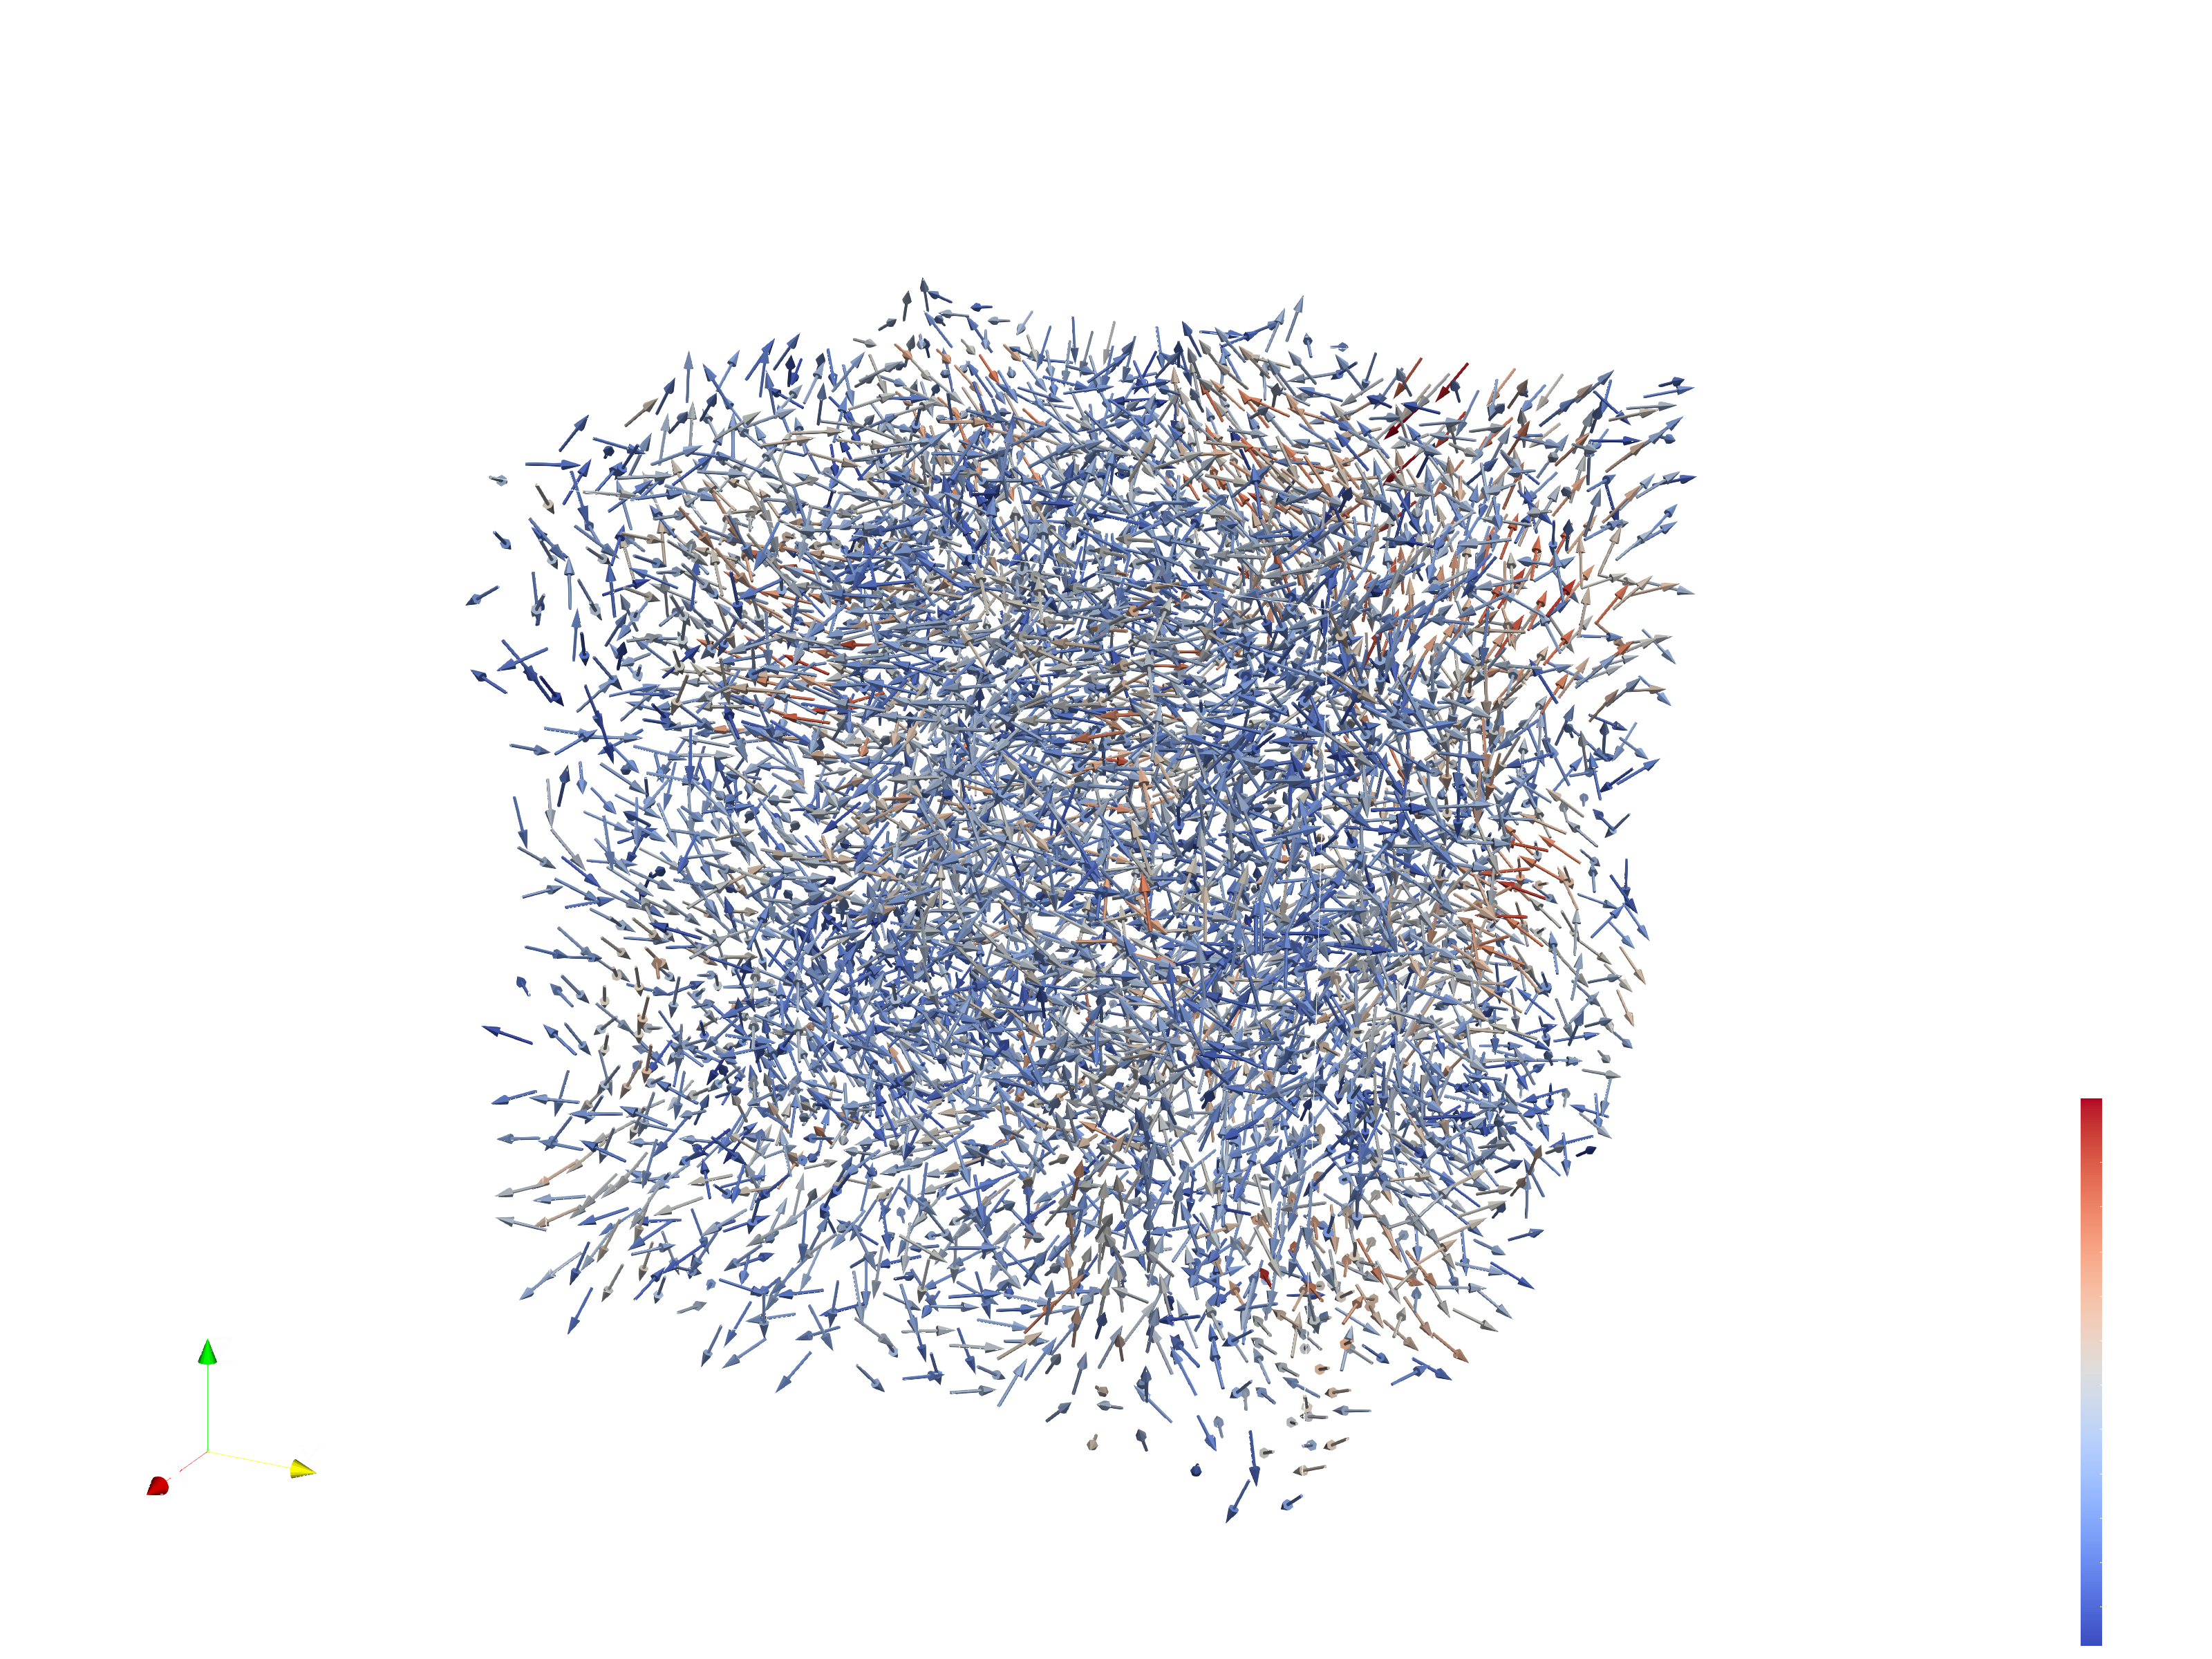
\includegraphics[width=0.45\linewidth]{images/kriging/3components/full_field_velocity_field.png}}%
        \hfill
        \subcaptionbox{плоскость $xy$, $z = 0$\label{img:slice_velociy_field_xy_znormal_angle_1}} 
        {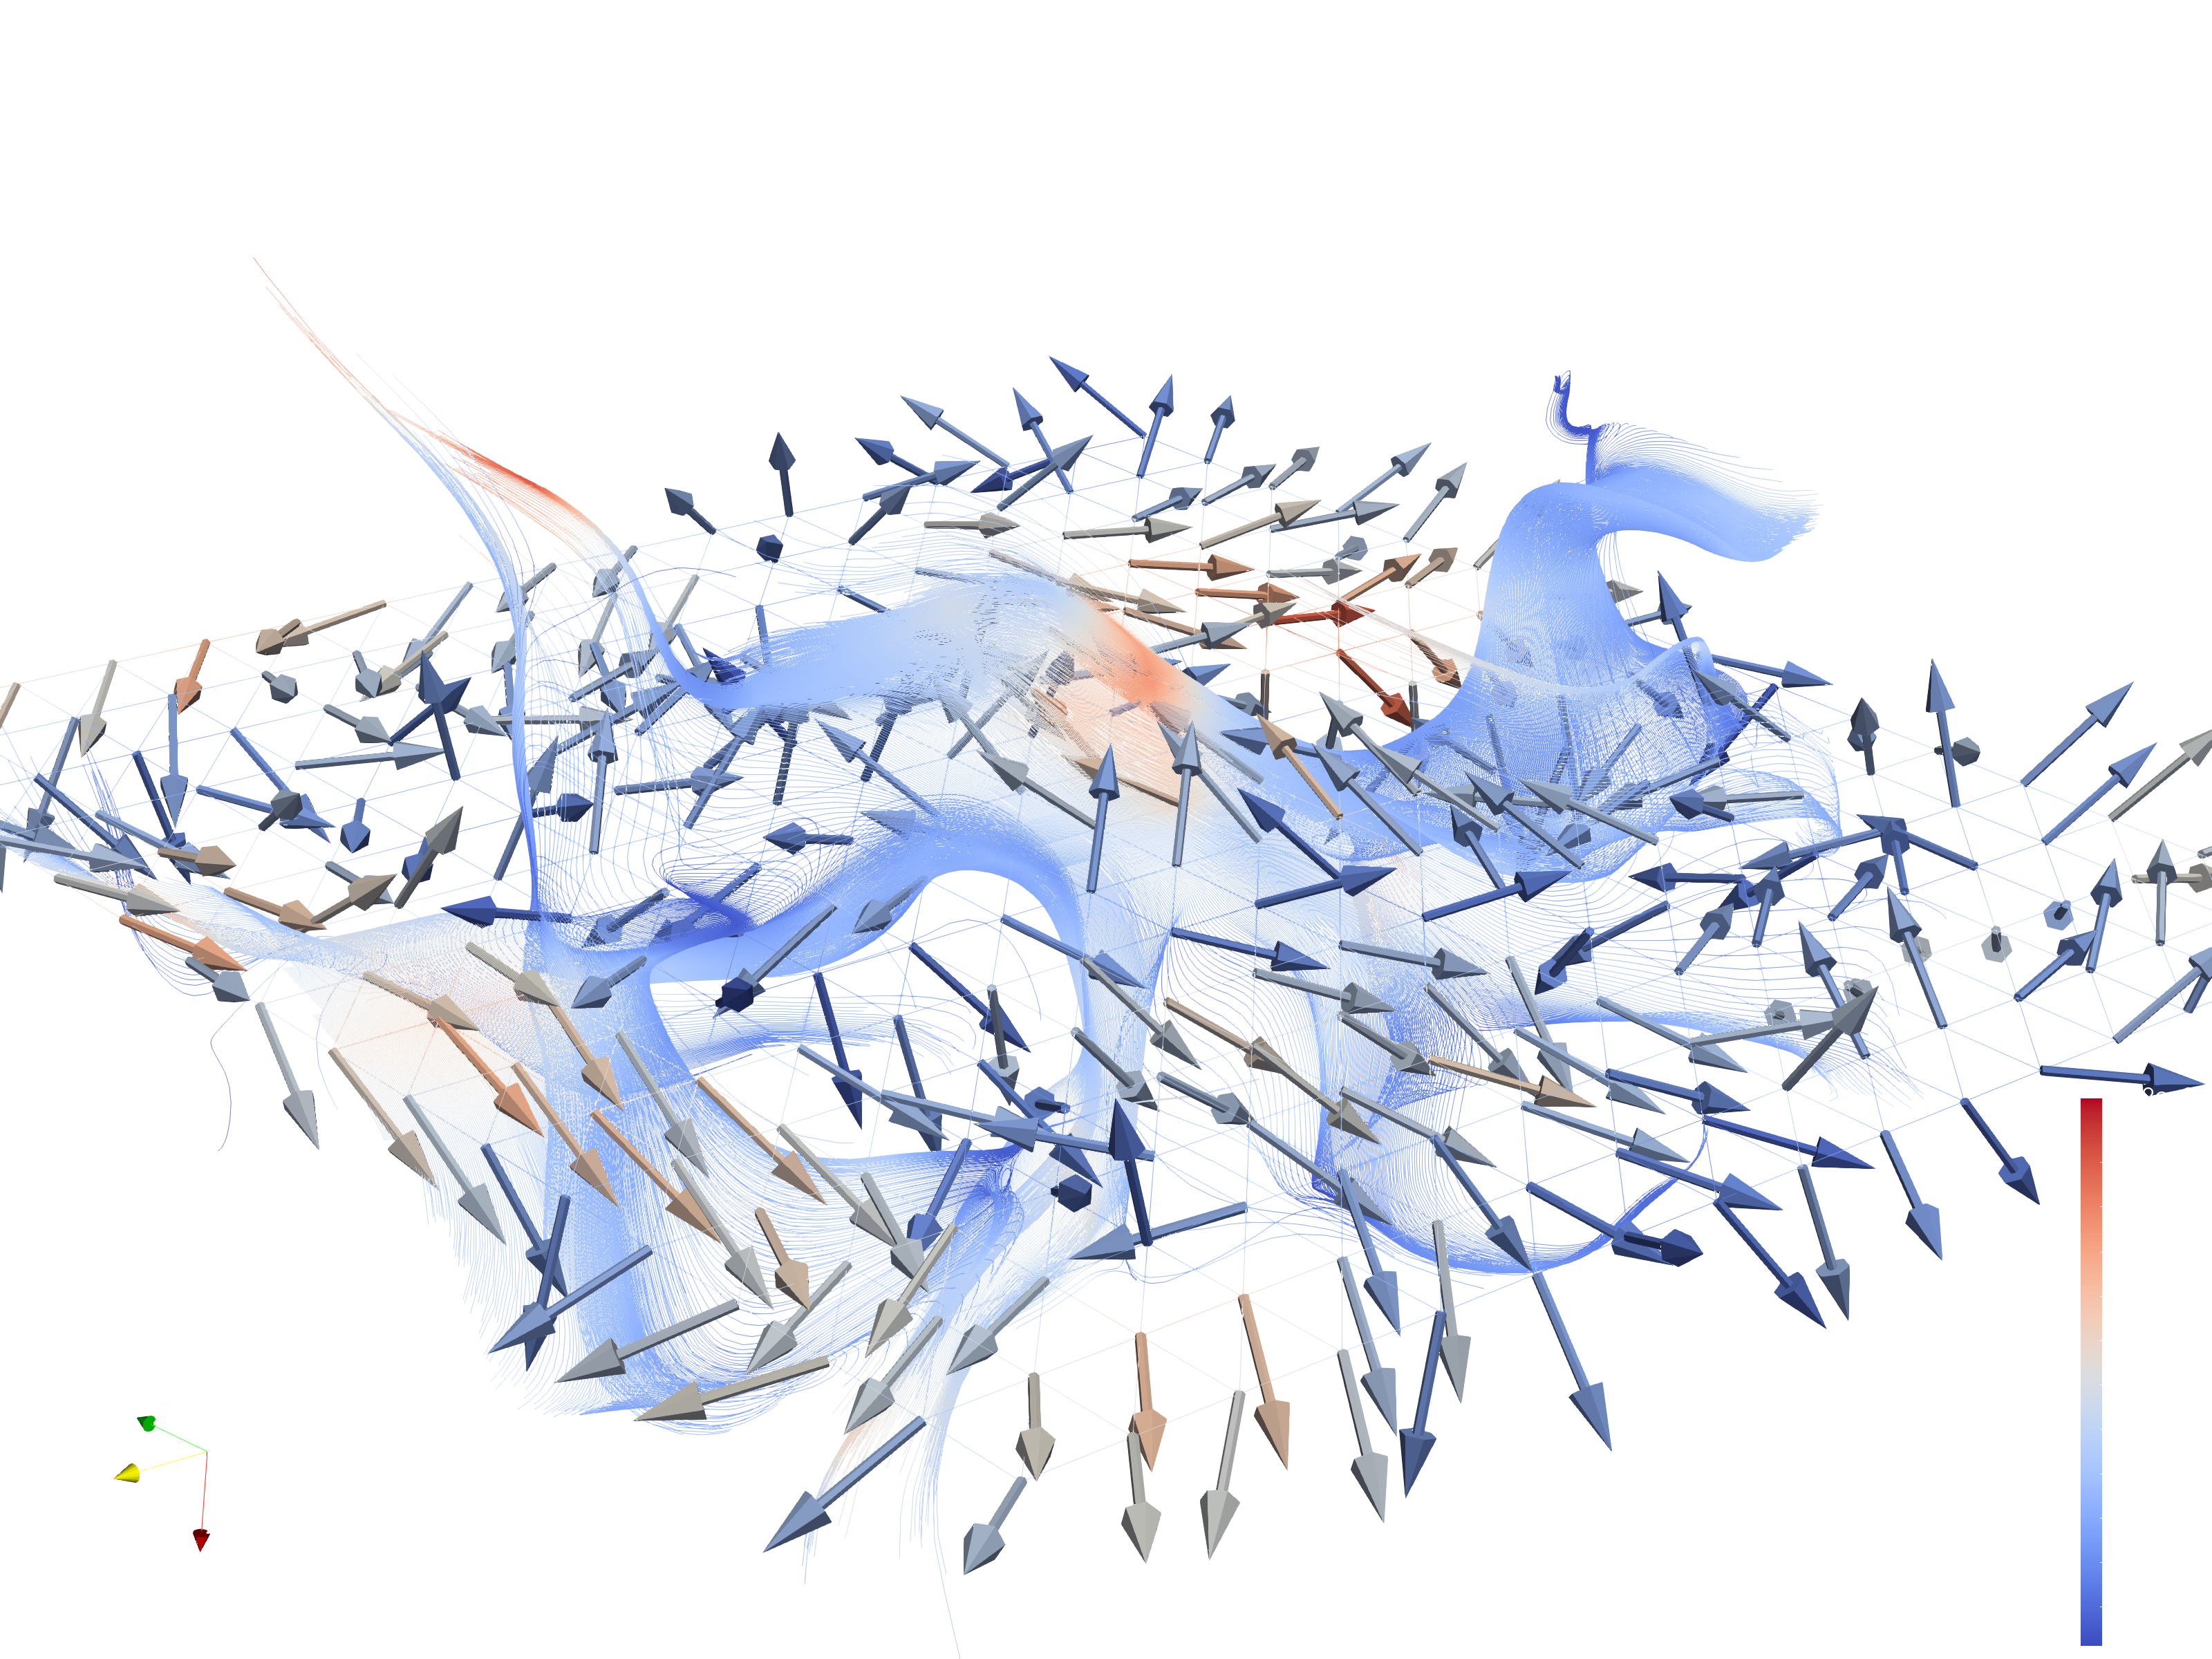
\includegraphics[width=0.45\linewidth]{images/kriging/3components/z_normal_xyplane_on_angle_with_stream_trace.png}} \\
    }
    \center{
        \subcaptionbox[List-of-Figures entry]{плоскость $xy$, $z = 0$\label{img:slice_velociy_field_xy_znormal_angle_2}} 
        {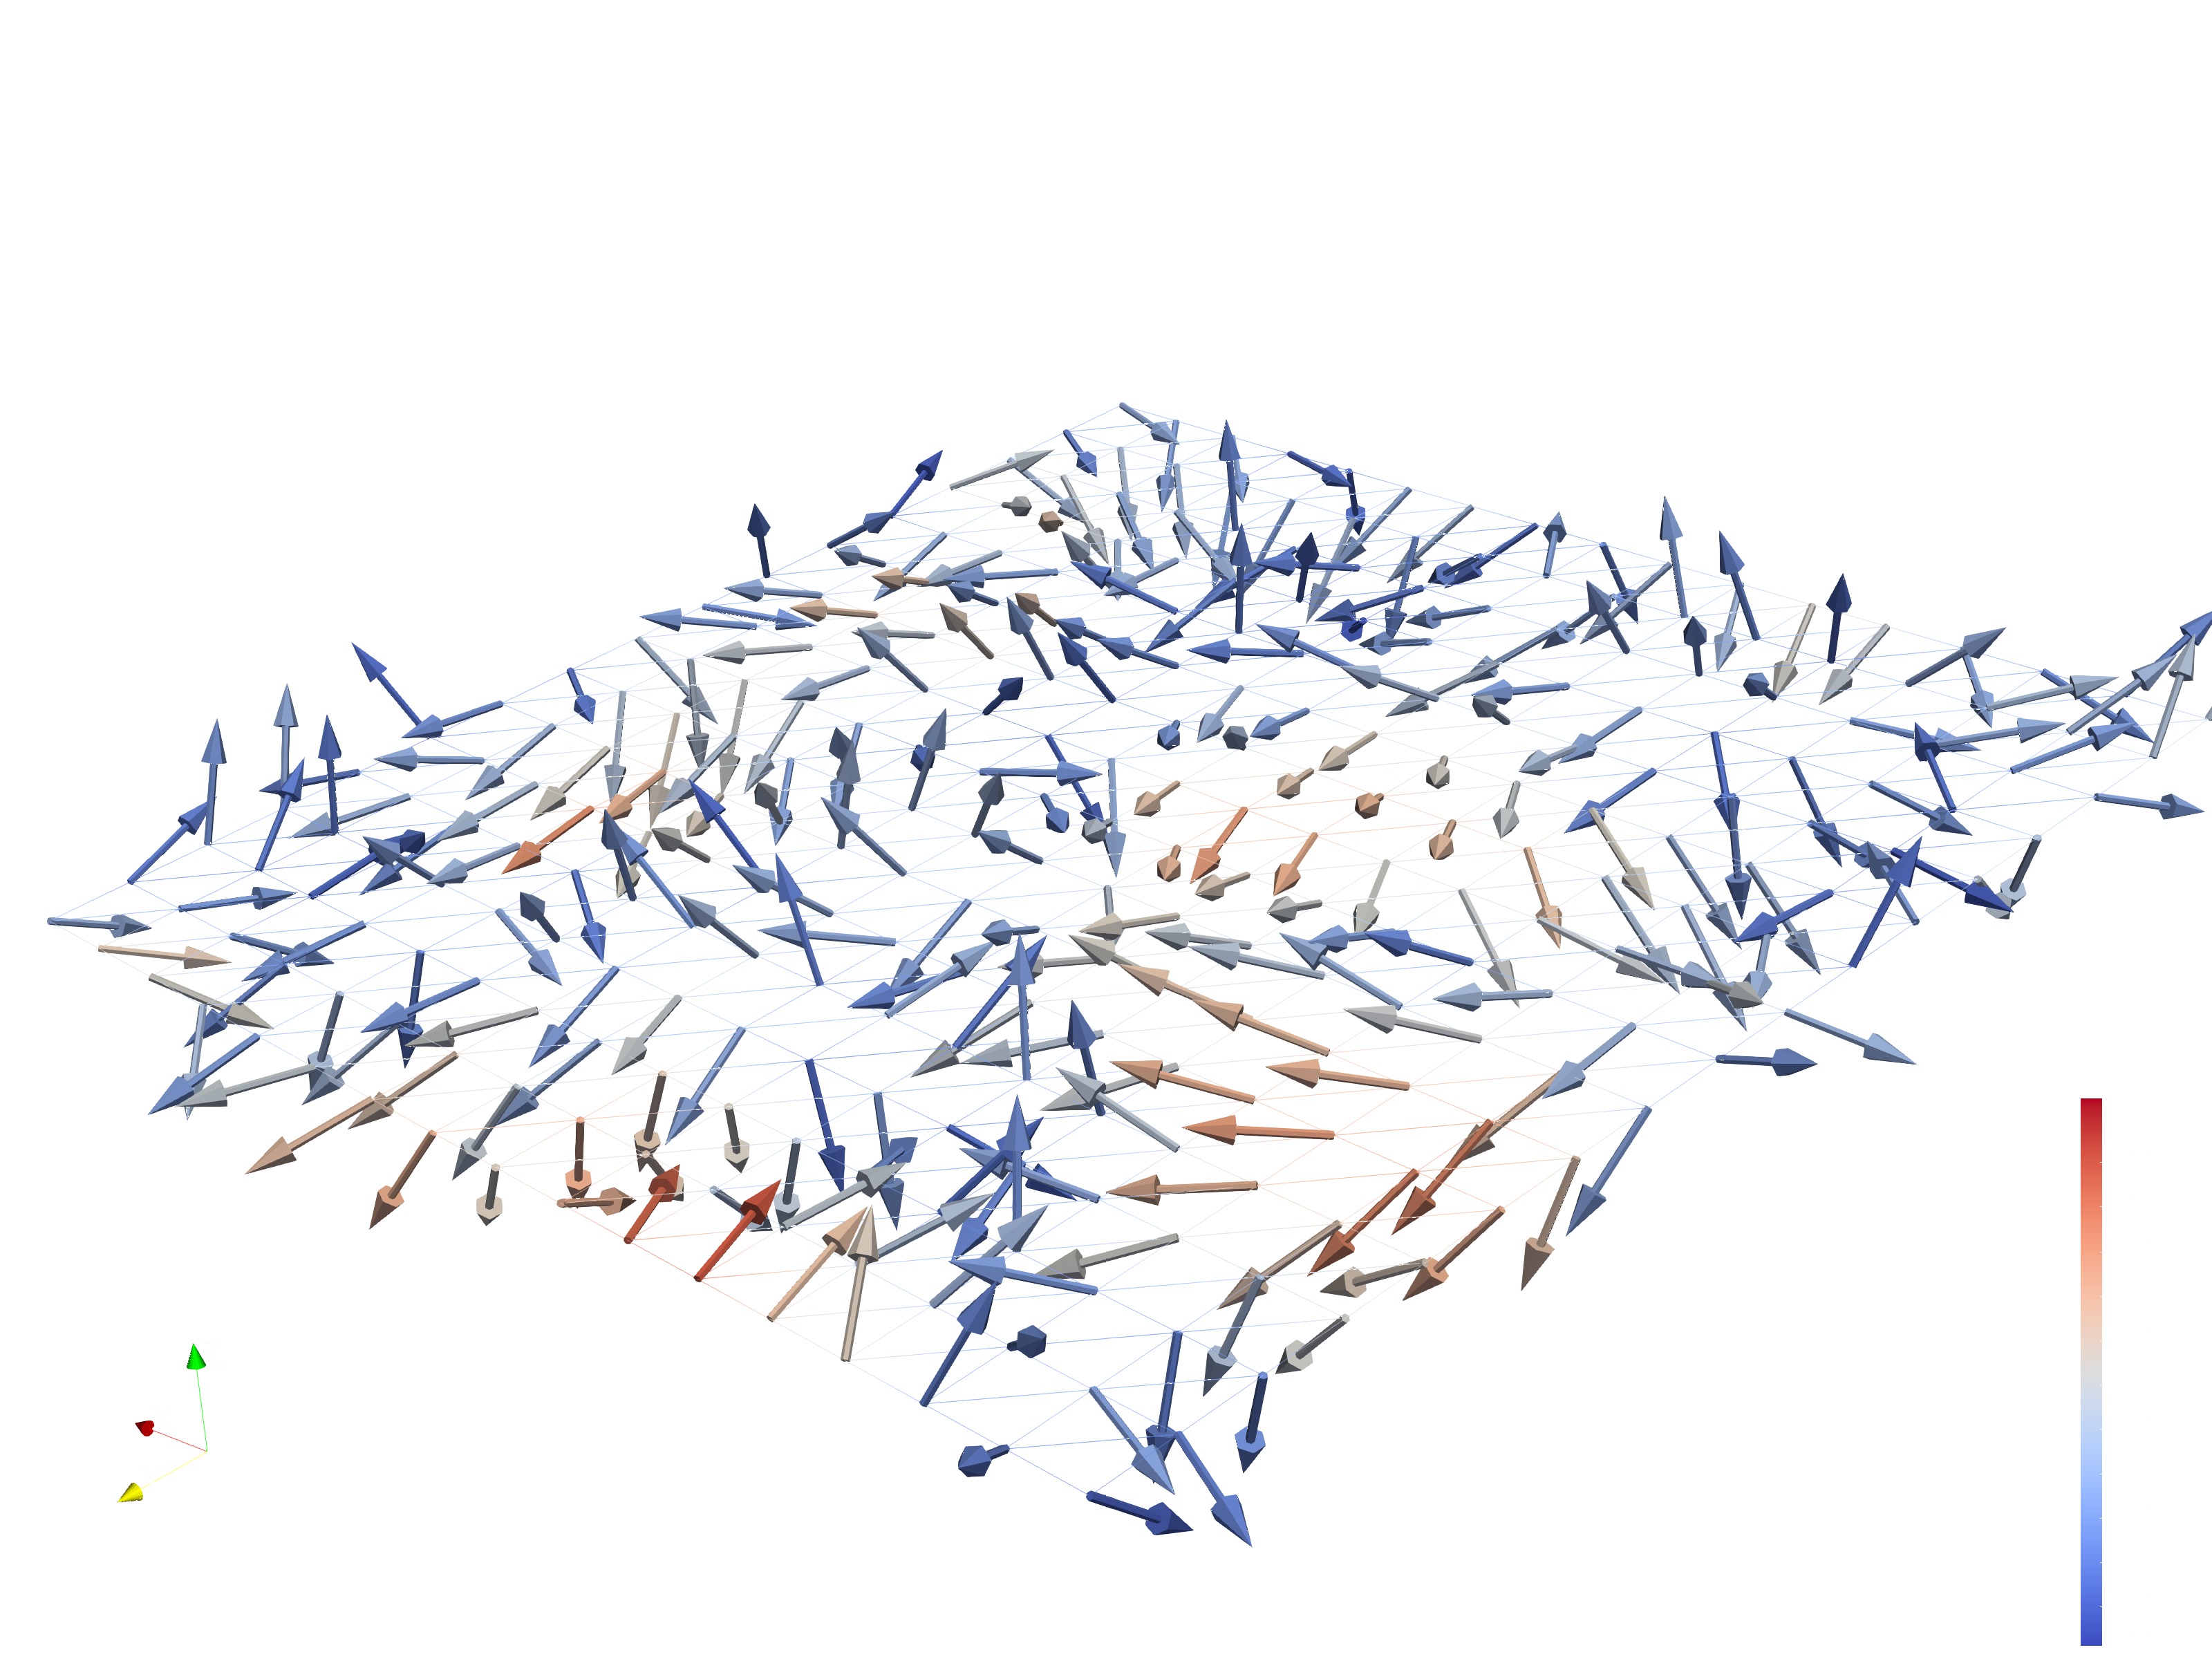
\includegraphics[width=0.45\linewidth]{images/kriging/3components/z_normal_xyplane_on_angle.png}}%
        \hfill
        \subcaptionbox{плоскость $xy$, $z = 0$\label{img:slice_velociy_field_xy_znormal_no_angle}} 
        {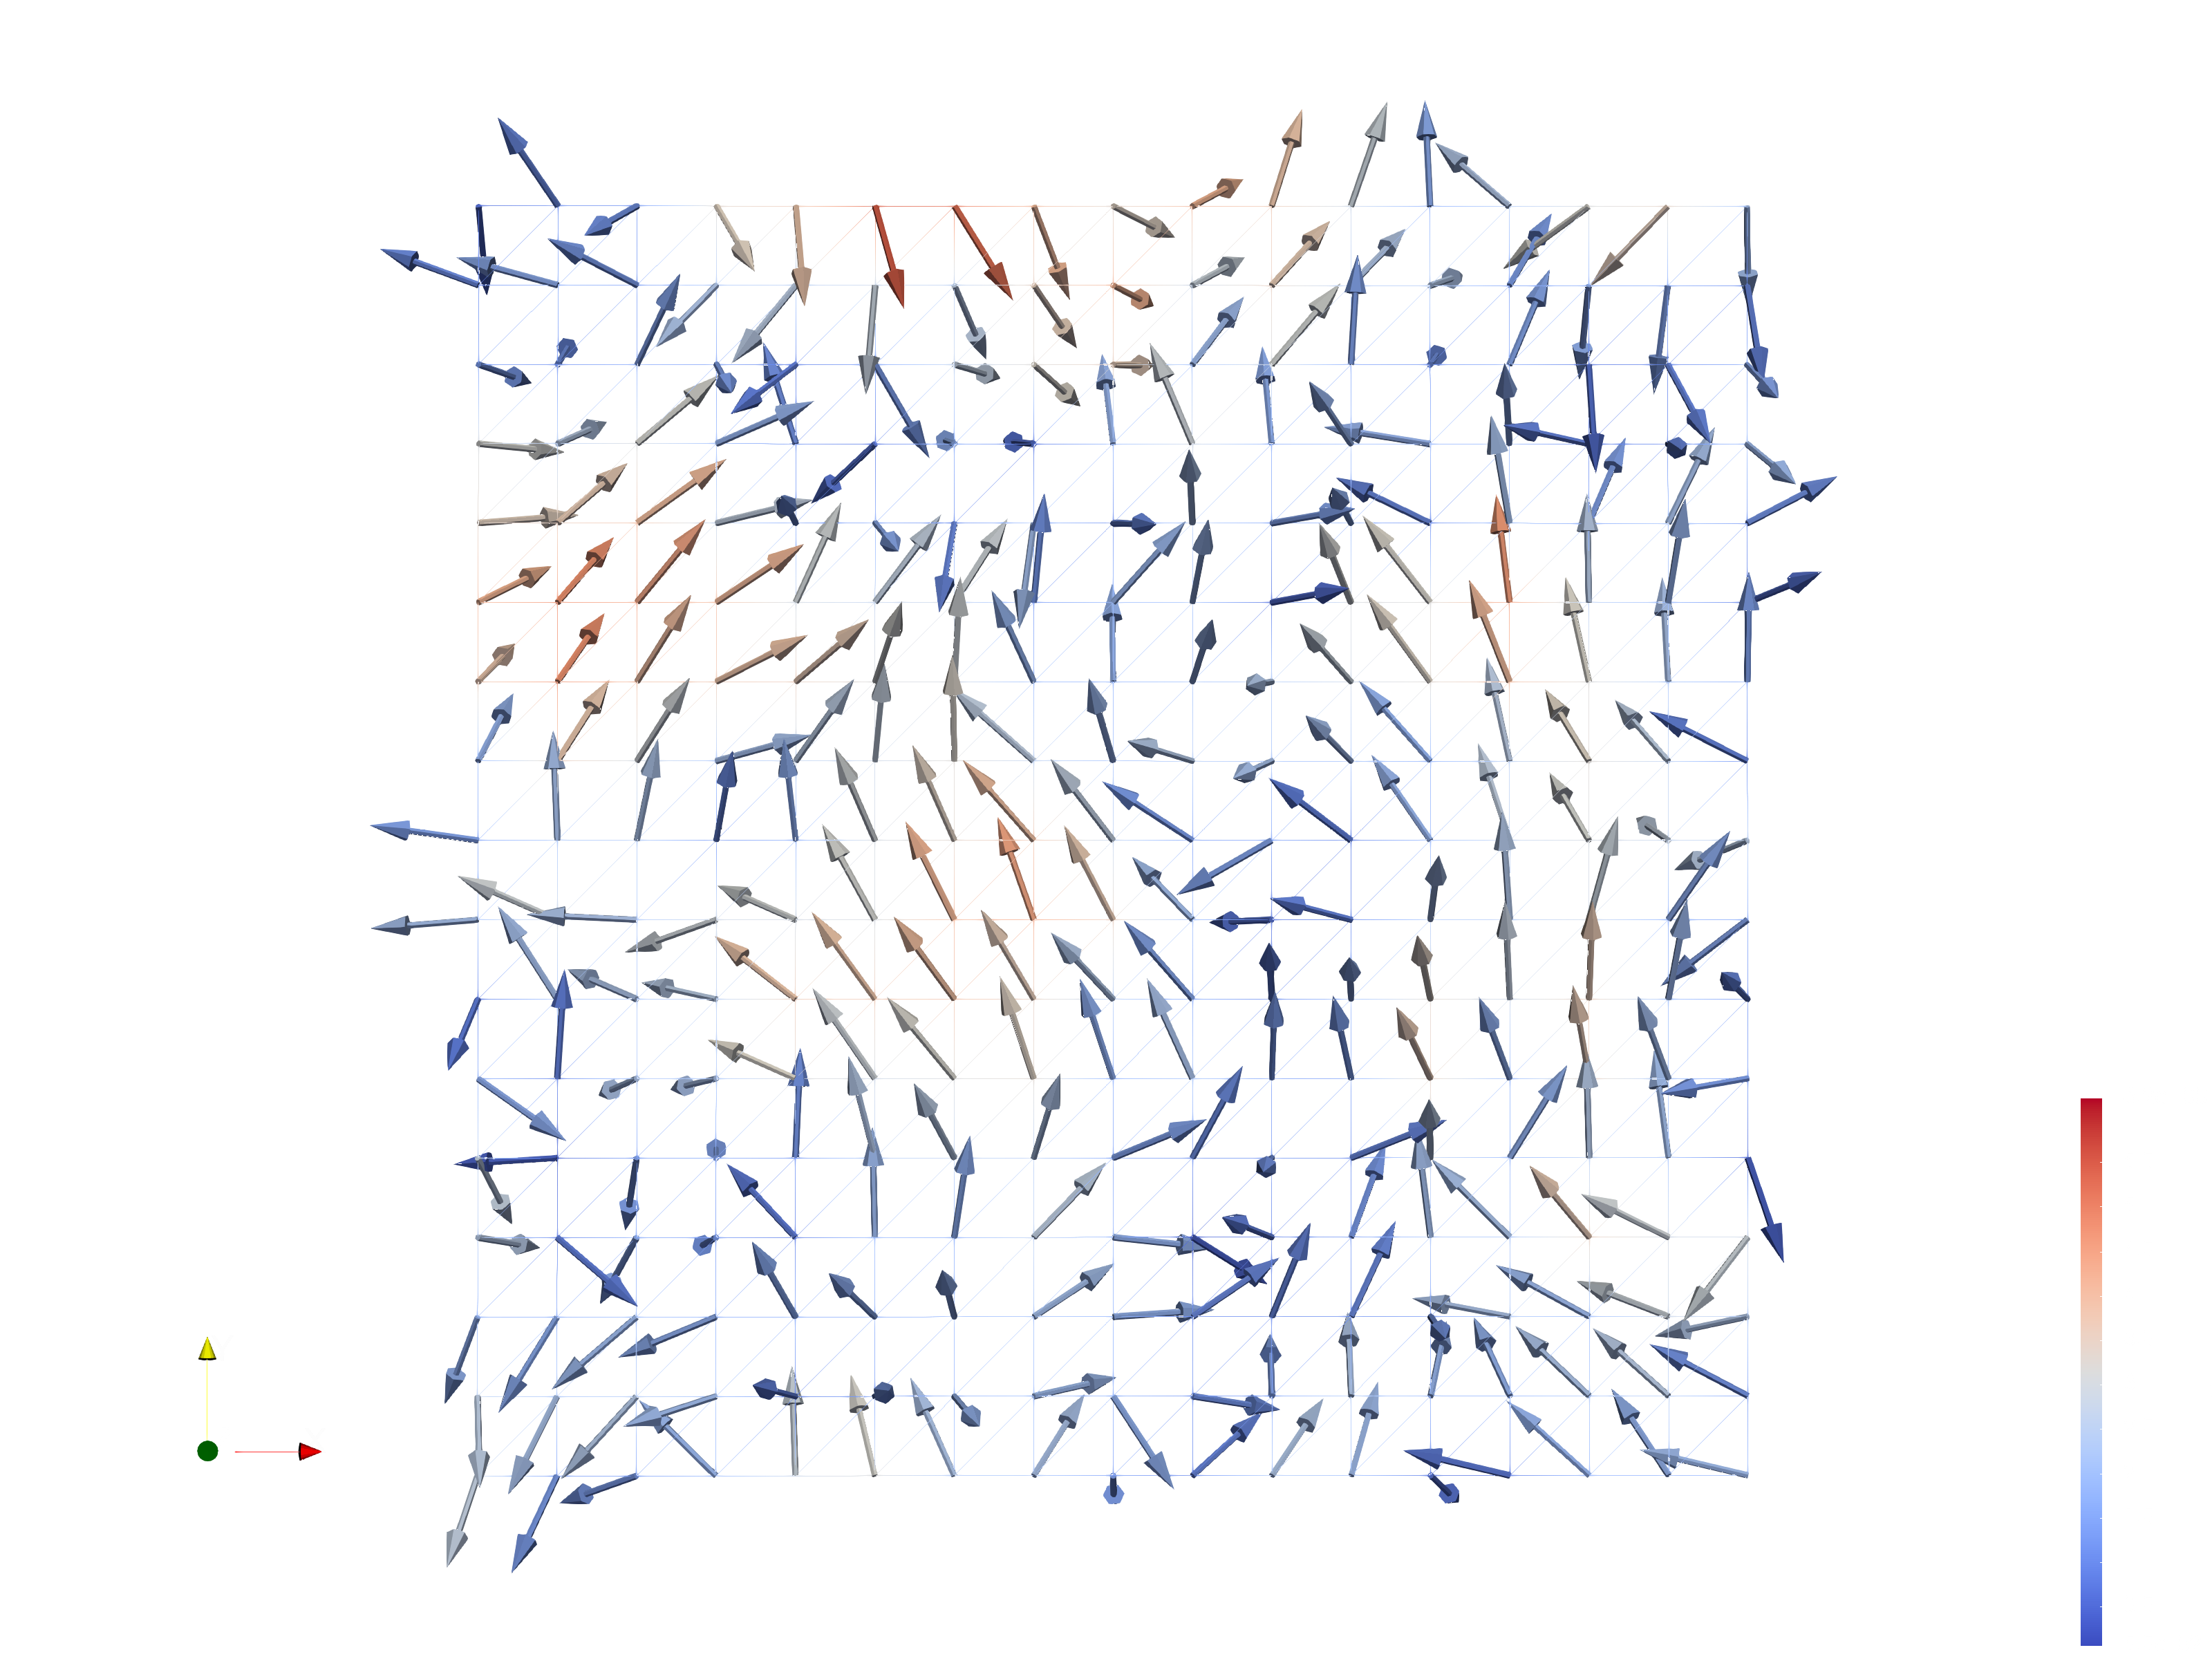
\includegraphics[width=0.45\linewidth]{images/kriging/3components/z_normal_xyplane.png}}

    }
    
    \onehalfspacing{Поле на картинке б представлено с линиями тока, расчитанными вдоль оси $y$}
    \caption{Поле флуктуаций сгенерированных трёхмерным стохастическим методом, цветом обозначена амплитуда флуктуаций}
    \label{img:velocity_fluctuation_field_for_kriging}  
\end{figure}

Приведём тепловые карты тензора ковариаций полученного из целевого спектра при помощи \eqref{eq:part3_2} и \eqref{eq:kriging_equation14_2}.

%
% Точная ковариация
%
\begin{figure}[!ht]
    \center{
        \subcaptionbox[List-of-Figures entry]{$R_{xx}$  $x$-нормаль\label{img:kriging_exact_cov_11_xx}} 
        {\includegraphics[width=0.32\linewidth]{images/kriging/3components/exact_cov_11_xx.png}}%
        \hfill
        \subcaptionbox{$R_{xx}$  $y$-нормаль \label{img:kriging_exact_cov_11_yy}} 
        {\includegraphics[width=0.32\linewidth]{images/kriging/3components/exact_cov_11_yy.png}}
        \hfill
        \subcaptionbox{$R_{xx}$  $z$-нормаль\label{img:kriging_exact_cov_11_zz}} 
        {\includegraphics[width=0.32\linewidth]{images/kriging/3components/exact_cov_11_zz.png}}%
    }
    \center{
        \subcaptionbox{$R_{yy}$ $x$-нормаль \label{img:kriging_exact_cov_22_xx}} 
        {\includegraphics[width=0.32\linewidth]{images/kriging/3components/exact_cov_22_xx.png}}
        \hfill
        \subcaptionbox{$R_{yy}$ $y$-нормаль \label{img:kriging_exact_cov_22_yy}} 
        {\includegraphics[width=0.32\linewidth]{images/kriging/3components/exact_cov_22_yy.png}}
        \hfill
        \subcaptionbox{$R_{yy}$ $z$-нормаль \label{img:kriging_exact_cov_22_zz}} 
        {\includegraphics[width=0.32\linewidth]{images/kriging/3components/exact_cov_22_zz.png}}
    }
    \center{       
        \subcaptionbox{$R_{zz}$ $x$-нормаль \label{img:kriging_exact_cov_33_xx}} 
        {\includegraphics[width=0.32\linewidth]{images/kriging/3components/exact_cov_33_xx.png}}
        \hfill
        \subcaptionbox{$R_{zz}$ $y$-нормаль \label{img:kriging_exact_cov_33_yy}} 
        {\includegraphics[width=0.32\linewidth]{images/kriging/3components/exact_cov_33_yy.png}}
        \hfill
        \subcaptionbox{$R_{zz}$ $z$-нормаль \label{img:kriging_exact_cov_33_zz}} 
        {\includegraphics[width=0.32\linewidth]{images/kriging/3components/exact_cov_33_zz.png}}
    }
    
    \onehalfspacing{}
    \caption{Ковариационные функции, заданные для применения трёхмерного стохастического метода}
    \label{img:exact_covariance_comparison_heat_maps}  
\end{figure}

Первое, что необходимо заметить, это пространственное вытягивание компонент тензора в смежных плоскостях, в плоскостях, нормальных к текущей компоненте наблюдается симметрия ковариационной функции. При сравнении с численно полученным результатом также учтём это. Вне диагональные компоненты не представлены, так как их значение можно считать нулевыми.

Ниже представлены графики пространственной ковариации рассчитанные на 10000 реализаций полей флуктуаций полученные в результате трёхмерного стохастического моделирования. На рисунках представлены значения вдоль диагонали куба от точки $\{-5, -5, -5\}$ до точки $\{ 5, 5, 5 \}$ и значения вдоль осей координат.

%
% Ковариация по осям координат
%
\begin{figure}[ht] 
  \center
  \includegraphics [width=0.8\linewidth] {images/kriging/3components/calculated_all_diag.png}
  \caption{Расчётная ковариационная функция $R_{ik}$ на основе стохастического метода вдоль диагонали области } 
  \label{img:kriging_covariances_diag}  
\end{figure}

\begin{figure}[ht] 
  \center
  \includegraphics [width=0.8\linewidth] {images/kriging/3components/calculated_all_x.png}
  \caption{Расчётная ковариационная функция $R_{ik}$ на основе стохастического метода вдоль оси $x$ области } 
  \label{img:kriging_covariances_x}  
\end{figure}

\begin{figure}[ht] 
  \center
  \includegraphics [width=0.8\linewidth] {images/kriging/3components/calculated_all_y.png}
  \caption{Расчётная ковариационная функция $R_{ik}$ на основе стохастического метода вдоль оси $y$ области } 
  \label{img:kriging_covariances_y}  
\end{figure}

\begin{figure}[ht] 
  \center
  \includegraphics [width=0.8\linewidth] {images/kriging/3components/calculated_all_z.png}
  \caption{Расчётная ковариационная функция $R_{ik}$ на основе стохастического метода вдоль оси $z$ области } 
  \label{img:kriging_covariances_y}  
\end{figure}

Как можно видеть из приведённых выше графиков, наблюдается вытягивание вдоль соответствующих компонент. Также наблюдается достаточно высокая визуальная симметрия относительно начала координат. С ростом расстояния наблюдаются большие отклонения ковариационной функции, связанные с тем, что выборка, на которой рассчитывались ковариационные функции конечна. Ниже представлены сравнения полученных ковариационны функций для диагональных компонент в различных направлениях с задаваемыми, а также с симметризованной относительно начала координат расчётной ковариационной функцией.

\begin{figure}[ht] 
  \center
  \includegraphics [width=0.8\linewidth] {images/kriging/3components/diagonal_r11_x.png}
  \caption{Расчётная ковариационная функция $R_{xx}$ на основе стохастического метода вдоль диагонали области } 
  \label{img:kriging_covariances_diagonal_r11_x}  
\end{figure}

\begin{figure}[ht] 
  \center
  \includegraphics [width=0.8\linewidth] {images/kriging/3components/diagonal_r22_yy.png}
  \caption{Расчётная ковариационная функция $R_{yy}$ на основе стохастического метода вдоль диагонали области } 
  \label{img:kriging_covariances_diagonal_r22_yy}  
\end{figure}

\begin{figure}[ht] 
  \center
  \includegraphics [width=0.8\linewidth] {images/kriging/3components/diagonal_r33_zz.png}
  \caption{Расчётная ковариационная функция $R_{zz}$ на основе стохастического метода вдоль диагонали области } 
  \label{img:kriging_covariances_diagonal_r33_zz}  
\end{figure}

По правой части графиков можно заметить насколько расчётная ковариационная функция не симметрична. Из-за этого дальнейшие расчёты тензора спектра скоростей и энергетического спектра проводились на симметризованной ковариационной функции. Процедура симметризации спектра необходима для устранения фазового смещения будущего тензора спектра скоростей, так как в ином случае при проведении преобразования Фурье, возникает мнимая часть, связанная с фазовым сдвигом, возникающим в следствии несимметричности функции, так как использовалось быстрое преобразование Фурье, требующее искусственного продолжения периодического сигнала. Возникающий скачок между продолженными ковариационными функциями, вносит фазовое смещение, откуда и возникает мнимая часть преобразования. Можно сказать, что мы рассматриваем не весь куб, а лишь его первый октант, данные для которого были симметрично продолжены относительно начала координат и граничащих плоскостей координат. 

Из-за мало корреляции компонент скоростей на больших расстояниях, также присутствуют большие отклонения ковариационной функции относительно задаваемой, что также вносит свою небольшую ошибку. Этот эффект отражается на последующем преобразовании Фурье при переходе от функций пространственной ковариации к тензору спектра скоростей. Ниже представлено сравнение расчётных значений тензора спектра скоростей с полученными применением формулы \eqref{eq:part3_2}. 
\noindent
\begin{figure}[!ht]
    \center{
        \subcaptionbox[List-of-Figures entry]{$R_{xx}$\label{img:kriging_computed_phi_11_diagonal}} 
        {\includegraphics[width=0.45\linewidth]{images/kriging/3components/phi_11_diagonal.png}}%
        \hfill
        \subcaptionbox{$R_{xy}$ и $R_{yx}$\label{img:kriging_computed_phi_12_diagonal}} 
        {\includegraphics[width=0.45\linewidth]{images/kriging/3components/phi_12_21_diagonal.png}} \\
    }
    \center{
        \subcaptionbox{$R_{xz}$ и $R_{zx}$\label{img:kriging_computed_phi_13_diagonal}} 
        {\includegraphics[width=0.45\linewidth]{images/kriging/3components/phi_13_31_diagonal.png}}
        \hfill
        \subcaptionbox{$R_{yy}$\label{img:kriging_computed_phi_22_diagonal}} 
        {\includegraphics[width=0.45\linewidth]{images/kriging/3components/phi_22_diagonal.png}} \\
    }
    \center{
        \subcaptionbox{$R_{yz}$ и $R_{yz}$\label{img:kriging_computed_phi_23_diagonal}} 
        {\includegraphics[width=0.45\linewidth]{images/kriging/3components/phi_23_32_diagonal.png}}
        \hfill
        \subcaptionbox{$R_{zz}$\label{img:kriging_computed_phi_33_diagonal}} 
        {\includegraphics[width=0.45\linewidth]{images/kriging/3components/phi_33_diagonal.png}}
    }
    
    \onehalfspacing{Функции тензора спектра энергий представлены дволь диагонали куба в пространстве фурье $n=17$, $k_l=10$}
    \caption{Ковариационные функции, заданные для применения трёхмерного стохастического метода}
    \label{img:exact_covariance_comparison_heat_maps_for_3d}  
\end{figure}

Как можно заметить, основные различия между вычисленными и заданными компонентами тензора присутствуют при $\Phi \approx 0$. Далее используя формулу \eqref{eq:part3_2} перейдём от тензора спектра скоростей к энергетическому спектру. 

\begin{figure}[ht] 
  \center
  \includegraphics [width=0.9\linewidth] {images/kriging/3components/energy_function_kriging_loglog.png}
  \caption{Энергетический спектр поля скоростей полученный в результате стохастического моделирования в сравнении с целевым спектром в логарифмических координатах} 
  \label{img:kriging_spectra_function_compare}  
\end{figure}

Полученный спектр хорошо сходится с целевым спектров области наиболее энергонесущих мод. Есть сходство со спектром получаемым в результате метода Крайшнана, в частности резкое убывание, предположительно связанное с критерием Нейквиста.

Рассмотрим генерацию поля флуктуаций с использованием последовательного моделирования. Как говорилось в \ref{chapt1}, в данном случае, основным параметров генерации, который мы можем варьировать -- число ближайших соседей, учитываемых при расчёта среднего и ковариации величины в точке. Наиболее оптимальным оказалось число $N=15$ при котором наблюдается хорошая аппроксимация целевого спектра, а также достаточно высокая производительность. Для обычного непоследовательного стохастического метода, помимо высокого затрачиваемого процессорного времени, требуется достаточно большой объём памяти, что может сильно ограничить возможность генерации на подробных сетках. В свою очередь, метод последовательных симуляций позволяет сократить требуемое количество памяти, за счёт отказа от хранения матрицы ковариаций целиком (теперь необходимо хранить матрицы $n \times n$). Малое число параметров, позволяет более простым образом задать требуемый спектр. Ниже представлено сравнение спектров, результирующего, полученного с использованием 1000 реализаций поля генерируемого последовательным методом. Параметры сеток задавалась следующими: для сетки пространства Фурье $l_F=20$, $n_F = 51$, для сетки физического пространства $n_{P} = 31$, $l=10$. Число учитываемых ближайших соседей $N = 15$.

\begin{figure}[ht] 
    \center
    \includegraphics [width=0.8\linewidth] {images/kriging/spectrum.png}
    \caption{Сравнение энергетического спектра для предлагаемой модификации спектрального метода с целевым} 
    \label{img:kriging_result_field_no_angle}  
\end{figure}

\begin{figure}[ht] 
    \center
    \includegraphics [width=0.8\linewidth] {images/kriging/spectrum_loglog.png}
    \caption{Сравнение энергетического спектра для предлагаемой модификации спектрального метода с целевым в логарифмических координатах} 
    \label{img:kriging_result_field_on_angle}  
\end{figure}

Как и в случае спектрального метода, наблюдается разница в спектрах для малых волновых чисел, в остальном, особенно в инерционном интервале, получаем практически точное сходство. Наибольшее отклонение результирующего от задаваемого спектров $\Delta E = 0.025$, но также стоит отметить, что это значение находится в волновых числах меньше чем минимальное волновое число на сетке $k_{min}=\frac{2 \pi}{10} \approx 0.628$. Как было сказано выше основным критерием выбора метода является удовлетворению целевому спектру. Рассмотрим сравнение полученных спектров обоими методами с целевым спектром.

\begin{figure}[ht] 
    \center
    \includegraphics [width=0.8\linewidth] {images/comparison_of_result_spectras.png}
    \caption{Сравнение энергетического спектра для предлагаемой модификации спектрального метода с целевым в логарифмических координатах} 
    \label{img:main_comparison_of_target_spectras}  
\end{figure}

Для полей получаемых по результатам спектрального метода, наблюдается лучшая точность при малых волновых числах, с учётом того что существуют ограничения на волновые числа многократно описанные выше. Метод последовательных симуляций лучшим образом аппроксимирует спектр в инерционном интервале, а также имеет более точное совпадение пика для наиболее энергонесущей волны. Но по сравнению со спектральным методом, данный имеет большее затрачиваемое время на одну реализацию. С сетки и параметра $N$ описанных выше, генерация 1000 полей происходит за 2 минуты 14 секунд, одна реализация требует $\frac{134}{1000} \approx 0.134$ секунд, без учёта времени на запись результатов, результат больше чем требуется для спектрального метода в 3 раза.

Рассмотрим также ковариационную функцию, рассчитанную на 5000 реализациях поля флуктуаций по методу последовательных симуляций. 

\begin{figure}[ht] 
    \center
    \includegraphics [width=0.8\linewidth] {images/kriging/covariance_tensor.png}
    \caption{Сравнение расчётных значений тензора ковариаций и входных вдоль диагонали куба} 
    \label{img:main_comparison_of_target_cov_function_and_computed}  
\end{figure}

Как мы видим, форма ковариаций сохраняется, но амплитуда меньше чем должна быть. По аналогии с обычным стохастическим методом из-за ограничения числа взятых соседей (в том случае числа собственных чисел и векторов) наблюдается различие между данными функциями, чем большее число мы будем рассматривать тем ближе будем приближаться к точной функции ковариации. То-есть мы можем сэкономить вычислительное время и ресурсы в конечном итоге имея хорошую аппроксимацию целевого спектра.

Хоть для метода последовательных симуляций не было явного учета удовлетворению условию неразрывности, рассмотрим его и для данного метода, так как это также один из критериев генерации более реалистичной турбулентности. По аналогии со спектральным методом рассчитаем величину $\vec \nabla \cdot \vec v$ характеризующее отклонение от данного закона. 

\begin{figure}[ht] 
    \center
    \includegraphics [width=0.8\linewidth] {images/kriging/velocity_components.png}
    \caption{Колебания компонент флуктуаций вдоль диагонали куба} 
    \label{img:sequential_method_velocity_components_along_diagonal}  
\end{figure}

\begin{figure}[ht] 
    \center
    \includegraphics [width=0.8\linewidth] {images/kriging/divergence.png}
    \caption{Сумма $\frac{\partial v_x}{\partial x} + \frac{\partial v_y}{\partial y} + \frac{\partial v_z}{\partial z}$ вдоль диагонали куба} 
    \label{img:sequential_method_velocity_field_divergence}  
\end{figure}

По сравнению со спектральным методом, наблюдаются большие величины отклонений от нулевого значения. Осредненное значение по объёму $<\vec \nabla \cdot \vec v> \approx -5.379 \cdot 10^{-3}$, средние значения компонент $\langle v_x \rangle \approx -5.384 \cdot 10^{-3}$, $\langle v_y \rangle \approx -0.843 \cdot 10^{-3} $, $\langle v_z \rangle \approx -5.206 \cdot 10^{-3}$. Среднее отклонение дивергенции больше чем в рассматриваемом спектральном методе, но стоит отметить более близкое значение среднего для компонент флуктуаций к 0;
           % Глава 3
%\chapter*{Заключение}						% Заголовок
\addcontentsline{toc}{chapter}{Заключение}	% Добавляем его в оглавление

%% Согласно ГОСТ Р 7.0.11-2011:
%% 5.3.3 В заключении диссертации излагают итоги выполненного исследования, рекомендации, перспективы дальнейшей разработки темы.
%% 9.2.3 В заключении автореферата диссертации излагают итоги данного исследования, рекомендации и перспективы дальнейшей разработки темы.
%% Поэтому имеет смысл сделать эту часть общей и загрузить из одного файла в автореферат и в диссертацию:

%% Согласно ГОСТ Р 7.0.11-2011:
%% 5.3.3 В заключении диссертации излагают итоги выполненного исследования, рекомендации, перспективы дальнейшей разработки темы.
%% 9.2.3 В заключении автореферата диссертации излагают итоги данного исследования, рекомендации и перспективы дальнейшей разработки темы.

По итогам данной диссертационной работы были реализованы и усовершенствованы подходы к генерации синтетической турбулентности. 

Первый из них основан на широкораспространённом спектральном методе. Предлагаемые усовершенствования нацелены не только на ускорение вычислительного алгоритма, но также и на лучшее удовлетворение целевым условиям, в виде лучшей аппроксимации задаваемого спектра. Переход к использованию одной гармоники Фурье позволяет существуенно сократить вычислительные затраты на генерацию одной флуктуации. Явное выражение амплитуд мод Фурье с использованием энергетического спектра позволяет проводить более точную аппроксимацию спектра, что в свою очередь ведёт к более реалистичному генерируемому полю турбулентных флуктуаций.

Метод последовательных симуляций ранее не использовался для генерации турбулентных флуктуаций, таким образом необходимо уделить особое внимание валидации генерируемых полей. Так, в сравнении с модифицированным спектральным методом мы показали, что данный предлагаемый подход является конкуретным для подобного рода задач, на примере совпадения целевого спектра, как главного критерия валидации. Последовательные симуляции позволили не только в разы сократить требуемое для генерации время, но также позволили рассматривать более подробные сетки и генерировать на них турбулентные флуктуации за счёт существенного уменьшения размерности результирующих матриц. Метод показал отличное совпадение с целевым спектром в инерционном интервале и показал более точное совпадение по сравнению со спектральным методом. 

Суммируя полученные результаты, кратко выделим преимущества и недостатки рассматриваемых методов.

Спектральный метод достоинства:
\begin{enumerate}
    \item Высокая скорость генерации одной реализации, в среднем $44 мс$, без ипользования параллельных вычислений;
    \item Устойчивость к топологии сетки, нет зависимости от соседник узлов;
    \item Возможность генерации поля флуктуаций изменяющееся во времени;
\end{enumerate}

Спектральный метод недостатки:
\begin{enumerate}
    \item Точность аппроксимации целевого спектра требует подбора параметров;
    \item Большое количество параметров влияющих на результат генерации;
\end{enumerate}

Метод последовательных симуляций достоинства:
\begin{enumerate}
    \item Высокая точность аппроксимации целевого спектра в инерционном интервале;
    \item Хорошая устойчивость к топологии сетки.
\end{enumerate}

Метод последовательных симуляций недостатки:
\begin{enumerate}
    \item Меньшая точность аппроксимации целевого спектра в диапазоне малых волновых чисел;
    \item Нет возможности генерации полей флуктуаций во времени;
    \item Большее время генерации (~3 раза) по сравнению со спектральным методом.
\end{enumerate}

На данный момент сложно выделить более подходящий метод, который был бы универсален в любой ситуации. Если необходима более точная аппроксимация целевого спектра более предпочтительным явялется метод последовательных симуляций. Меньшее число параметров позволяет сконцетрироваться на их подборе для получения лучшего результата. В свою очередь, спектральный метод будет хорошо если имеется необходимость в быстрой генерации полей и имеется достаточное расстояние для развития турбулентности из синтетической к физической. 

Отдельным пунктом можно рассмотреть зависимость от времени. Мы можем использовать оба метода для генерации граничных условий, граница является некоторой поверхностью, тем самым мы можем интерпретировать одну из осей как время и снимать вектора флуктуаций с ортгональной к этой оси плоскости. Для специфических задач, в которых граница это сложная область, в которой затруднительно провести генерацию на её поверхности с последующими смещениями для моделирования течения времени, более предпочтительным будет является спектральный метод.

В результате работы были решены поставленные задачи, предложен новый подход к генерации синтетической турбулентности. Была написана баблиотека генерации описанными в работе методами и выложена как открытый проект под лицензией MIT.

Планами на дальнейшую работу являются решение недостатков каждого из методов, возможно их объединение для совмещения сильных сторон обоих методов: точность аппроксимации целевого спектра, возможность генерации полей флуктуации во времени -- в конечном итоге проведение моделирования процессов с использованием предложенных генераторов турбулентности.

      % Заключение
%\clearpage                                  % В том числе гарантирует, что список литературы в оглавлении будет с правильным номером страницы
\phantomsection
\addcontentsline{toc}{chapter}{\bibname}	% Добавляем список литературы в оглавление
%\hypersetup{ urlcolor=black }               % Ссылки делаем чёрными
%\providecommand*{\BibDash}{}                % В стилях ugost2008 отключаем использование тире как разделителя 
\urlstyle{rm}                               % ссылки URL обычным шрифтом
\insertbibliofull                          % Подключаем Bib-базы
\urlstyle{tt}                               % возвращаем установки шрифта ссылок URL
%\hypersetup{ urlcolor={urlcolor} }          % Восстанавливаем цвет ссылок      % Список литературы
% \chapter*{Список сокращений и условных обозначений}             % Заголовок
\addcontentsline{toc}{chapter}{Список сокращений и условных обозначений}  % Добавляем его в оглавление

\textbf{КЭН} - Кандидат экономических наук

\textbf{РАН} - Российская академия наук

\textbf{РИТЭГ} - Радиоизотопный термоэлектрический генератор

\textbf{PDF} - Portable Document Format
        % Список сокращений и условных обозначений
% \chapter*{Словарь терминов}             % Заголовок
\addcontentsline{toc}{chapter}{Словарь терминов}  % Добавляем его в оглавление

% \textbf{TeX} - Cистема компьютерной вёрстки, разработанная американским профессором информатики Дональдом Кнутом

% \textbf{Панграмма} - Короткий текст, использующий все или почти все буквы алфавита
      % Словарь терминов
% \clearpage
\phantomsection
\addcontentsline{toc}{chapter}{\listfigurename}
\listoffigures									% Список изображений


%%% Список таблиц %%%
% (ГОСТ Р 7.0.11-2011, 5.3.10)
\clearpage
\phantomsection
\addcontentsline{toc}{chapter}{\listtablename}
\listoftables									% Список таблиц
\newpage           % Списки таблиц и изображений (иллюстративный материал)
% \appendix
%% Правка оформления ссылок на приложения:
%http://tex.stackexchange.com/questions/56839/chaptername-is-used-even-for-appendix-chapters-in-toc
%http://tex.stackexchange.com/questions/59349/table-of-contents-with-chapter-and-appendix
%% требует двойной компиляции
\addtocontents{toc}{\def\protect\cftchappresnum{\appendixname{} }%
\setlength{\cftchapnumwidth}{\widthof{\cftchapfont\appendixname~Ш\cftchapaftersnum}}%
}
%% Оформление заголовков приложений ближе к ГОСТ:
\sectionformat{\chapter}[display]{% Параметры заголовков разделов в тексте
    label=\chaptertitlename\ \thechapter,% (ГОСТ Р 2.105, 4.3.6)
    labelsep=20pt,
}
\renewcommand\thechapter{\Asbuk{chapter}} % Чтобы приложения русскими буквами нумеровались
   % Предварительные настройки для правильного подключения Приложений
% \chapter{Примеры вставки листингов программного кода} \label{AppendixA}

% Для крупных листингов есть два способа. Первый красивый, но в нём могут быть проблемы с поддержкой кириллицы (у вас может встречаться в комментариях и
% печатаемых сообщениях), он представлен на листинге~\ref{list:hwbeauty}.
% %\renewcommand\FBbskip{-20pt} % если хотим притянуть что-то к плавающему окружению из floatrow
% \begin{ListingEnv}[H]% буква H означает Here, ставим здесь,
%     % элементы, которые нежелательно разрывать обычно не ставят
%     % посреди страницы: вместо H используется t (top, сверху страницы),
%     % или b (bottom) или p (page, на отдельной странице)
% %    \captionsetup{format=tablenocaption}% должен стоять до самого caption
% %    \thisfloatsetup{\capposition=top}%
%     \caption{Программа “Hello, world” на \protect\cpp}
%     % далее метка для ссылки:
%     \label{list:hwbeauty}
%     % окружение учитывает пробелы и табляции и приеняет их в сответсвии с настройкми
%     \begin{lstlisting}[language={[ISO]C++}]
% 	#include <iostream>
% 	using namespace std;

% 	int main() //кириллица в комментариях при xelatex и lualatex имеет проблемы с пробелами
% 	{
% 		cout << "Hello, world" << endl; //latin letters in commentaries
% 		system("pause");
% 		return 0;
% 	}
%     \end{lstlisting}
% \end{ListingEnv}%
% Второй не такой красивый, но без ограничений (см.~листинг~\ref{list:hwplain}).
% \begin{ListingEnv}[H]
%     \begin{Verb}
        
%         #include <iostream>
%         using namespace std;
        
%         int main() //кириллица в комментариях
%         {
%             cout << "Привет, мир" << endl;
%         }
%     \end{Verb}
%     \caption{Программа “Hello, world” без подсветки}
%     \label{list:hwplain}
% \end{ListingEnv}

% Можно использовать первый для вставки небольших фрагментов
% внутри текста, а второй для вставки полного
% кода в приложении, если таковое имеется.

% Если нужно вставить совсем короткий пример кода (одна или две строки), то выделение  линейками и нумерация может смотреться чересчур громоздко. В таких случаях можно использовать окружения \texttt{lstlisting} или \texttt{Verb} без \texttt{ListingEnv}. Приведём такой пример с указанием языка программирования, отличного от заданного по умолчанию:
% \begin{lstlisting}[language=Haskell]
% fibs = 0 : 1 : zipWith (+) fibs (tail fibs)
% \end{lstlisting}
% Такое решение~--- со вставкой нумерованных листингов покрупнее
% и вставок без выделения для маленьких фрагментов~--- выбрано,
% например, в книге Эндрю Таненбаума и Тодда Остина по архитектуре
% %компьютера~\autocite{TanAus2013} (см.~рис.~\ref{fig:tan-aus}).

% Наконец, для оформления идентификаторов внутри строк
% (функция \lstinline{main} и тому подобное) используется
% \texttt{lstinline} или, самое простое, моноширинный текст
% (\texttt{\textbackslash texttt}).


% Пример~\ref{list:internal3}, иллюстрирующий подключение переопределённого языка. Может быть полезным, если подсветка кода работает криво. Без дополнительного окружения, с подписью и ссылкой, реализованной встроенным средством.
% \begin{lstlisting}[language={Renhanced},caption={Пример листинга c подписью собственными средствами},label={list:internal3}]
% ## Caching the Inverse of a Matrix

% ## Matrix inversion is usually a costly computation and there may be some
% ## benefit to caching the inverse of a matrix rather than compute it repeatedly
% ## This is a pair of functions that cache the inverse of a matrix.

% ## makeCacheMatrix creates a special "matrix" object that can cache its inverse

% makeCacheMatrix <- function(x = matrix()) {#кириллица в комментариях при xelatex и lualatex имеет проблемы с пробелами
%     i <- NULL
%     set <- function(y) {
%         x <<- y
%         i <<- NULL
%     }
%     get <- function() x
%     setSolved <- function(solve) i <<- solve
%     getSolved <- function() i
%     list(set = set, get = get,
%     setSolved = setSolved,
%     getSolved = getSolved)
    
% }


% ## cacheSolve computes the inverse of the special "matrix" returned by
% ## makeCacheMatrix above. If the inverse has already been calculated (and the
% ## matrix has not changed), then the cachesolve should retrieve the inverse from
% ## the cache.

% cacheSolve <- function(x, ...) {
%     ## Return a matrix that is the inverse of 'x'
%     i <- x$getSolved()
%     if(!is.null(i)) {
%         message("getting cached data")
%         return(i)
%     }
%     data <- x$get()
%     i <- solve(data, ...)
%     x$setSolved(i)
%     i  
% }
% \end{lstlisting} %$ %Комментарий для корректной подсветки синтаксиса
%                  %вне листинга

% Листинг~\ref{list:external1} подгружается из внешнего файла. Приходится загружать без окружения дополнительного. Иначе по страницам не переносится.
%     \lstinputlisting[lastline=78,language={R},caption={Листинг из внешнего файла},label={list:external1}]{listings/run_analysis.R}






% \chapter{Очень длинное название второго приложения, в котором продемонстрирована работа с длинными таблицами} \label{AppendixB}

%  \section{Подраздел приложения}\label{AppendixB1}
% Вот размещается длинная таблица:
% \fontsize{10pt}{10pt}\selectfont
% \begin{longtable}[c]{|l|c|l|l|}
% % \caption{Описание входных файлов модели}\label{Namelists} 
% %\\ 
%  \hline
%  %\multicolumn{4}{|c|}{\textbf{Файл puma\_namelist}}        \\ \hline
%  Параметр & Умолч. & Тип & Описание               \\ \hline
%                                               \endfirsthead   \hline
%  \multicolumn{4}{|c|}{\small\slshape (продолжение)}        \\ \hline
%  Параметр & Умолч. & Тип & Описание               \\ \hline
%                                               \endhead        \hline
% % \multicolumn{4}{|c|}{\small\slshape (окончание)}        \\ \hline
% % Параметр & Умолч. & Тип & Описание               \\ \hline
% %                                             \endlasthead        \hline
%  \multicolumn{4}{|r|}{\small\slshape продолжение следует}  \\ \hline
%                                               \endfoot        \hline
%                                               \endlastfoot
%  \multicolumn{4}{|l|}{\&INP}        \\ \hline 
%  kick & 1 & int & 0: инициализация без шума ($p_s = const$) \\
%       &   &     & 1: генерация белого шума                  \\
%       &   &     & 2: генерация белого шума симметрично относительно \\
%   & & & экватора    \\
%  mars & 0 & int & 1: инициализация модели для планеты Марс     \\
%  kick & 1 & int & 0: инициализация без шума ($p_s = const$) \\
%       &   &     & 1: генерация белого шума                  \\
%       &   &     & 2: генерация белого шума симметрично относительно \\
%   & & & экватора    \\
%  mars & 0 & int & 1: инициализация модели для планеты Марс     \\
% kick & 1 & int & 0: инициализация без шума ($p_s = const$) \\
%       &   &     & 1: генерация белого шума                  \\
%       &   &     & 2: генерация белого шума симметрично относительно \\
%   & & & экватора    \\
%  mars & 0 & int & 1: инициализация модели для планеты Марс     \\
% kick & 1 & int & 0: инициализация без шума ($p_s = const$) \\
%       &   &     & 1: генерация белого шума                  \\
%       &   &     & 2: генерация белого шума симметрично относительно \\
%   & & & экватора    \\
%  mars & 0 & int & 1: инициализация модели для планеты Марс     \\
% kick & 1 & int & 0: инициализация без шума ($p_s = const$) \\
%       &   &     & 1: генерация белого шума                  \\
%       &   &     & 2: генерация белого шума симметрично относительно \\
%   & & & экватора    \\
%  mars & 0 & int & 1: инициализация модели для планеты Марс     \\
% kick & 1 & int & 0: инициализация без шума ($p_s = const$) \\
%       &   &     & 1: генерация белого шума                  \\
%       &   &     & 2: генерация белого шума симметрично относительно \\
%   & & & экватора    \\
%  mars & 0 & int & 1: инициализация модели для планеты Марс     \\
% kick & 1 & int & 0: инициализация без шума ($p_s = const$) \\
%       &   &     & 1: генерация белого шума                  \\
%       &   &     & 2: генерация белого шума симметрично относительно \\
%   & & & экватора    \\
%  mars & 0 & int & 1: инициализация модели для планеты Марс     \\
% kick & 1 & int & 0: инициализация без шума ($p_s = const$) \\
%       &   &     & 1: генерация белого шума                  \\
%       &   &     & 2: генерация белого шума симметрично относительно \\
%   & & & экватора    \\
%  mars & 0 & int & 1: инициализация модели для планеты Марс     \\
% kick & 1 & int & 0: инициализация без шума ($p_s = const$) \\
%       &   &     & 1: генерация белого шума                  \\
%       &   &     & 2: генерация белого шума симметрично относительно \\
%   & & & экватора    \\
%  mars & 0 & int & 1: инициализация модели для планеты Марс     \\
% kick & 1 & int & 0: инициализация без шума ($p_s = const$) \\
%       &   &     & 1: генерация белого шума                  \\
%       &   &     & 2: генерация белого шума симметрично относительно \\
%   & & & экватора    \\
%  mars & 0 & int & 1: инициализация модели для планеты Марс     \\
% kick & 1 & int & 0: инициализация без шума ($p_s = const$) \\
%       &   &     & 1: генерация белого шума                  \\
%       &   &     & 2: генерация белого шума симметрично относительно \\
%   & & & экватора    \\
%  mars & 0 & int & 1: инициализация модели для планеты Марс     \\
% kick & 1 & int & 0: инициализация без шума ($p_s = const$) \\
%       &   &     & 1: генерация белого шума                  \\
%       &   &     & 2: генерация белого шума симметрично относительно \\
%   & & & экватора    \\
%  mars & 0 & int & 1: инициализация модели для планеты Марс     \\
% kick & 1 & int & 0: инициализация без шума ($p_s = const$) \\
%       &   &     & 1: генерация белого шума                  \\
%       &   &     & 2: генерация белого шума симметрично относительно \\
%   & & & экватора    \\
%  mars & 0 & int & 1: инициализация модели для планеты Марс     \\
% kick & 1 & int & 0: инициализация без шума ($p_s = const$) \\
%       &   &     & 1: генерация белого шума                  \\
%       &   &     & 2: генерация белого шума симметрично относительно \\
%   & & & экватора    \\
%  mars & 0 & int & 1: инициализация модели для планеты Марс     \\
% kick & 1 & int & 0: инициализация без шума ($p_s = const$) \\
%       &   &     & 1: генерация белого шума                  \\
%       &   &     & 2: генерация белого шума симметрично относительно \\
%   & & & экватора    \\
%  mars & 0 & int & 1: инициализация модели для планеты Марс     \\
%  \hline
%   %& & & $\:$ \\ 
%  \multicolumn{4}{|l|}{\&SURFPAR}        \\ \hline
% kick & 1 & int & 0: инициализация без шума ($p_s = const$) \\
%       &   &     & 1: генерация белого шума                  \\
%       &   &     & 2: генерация белого шума симметрично относительно \\
%   & & & экватора    \\
%  mars & 0 & int & 1: инициализация модели для планеты Марс     \\
% kick & 1 & int & 0: инициализация без шума ($p_s = const$) \\
%       &   &     & 1: генерация белого шума                  \\
%       &   &     & 2: генерация белого шума симметрично относительно \\
%   & & & экватора    \\
%  mars & 0 & int & 1: инициализация модели для планеты Марс     \\
% kick & 1 & int & 0: инициализация без шума ($p_s = const$) \\
%       &   &     & 1: генерация белого шума                  \\
%       &   &     & 2: генерация белого шума симметрично относительно \\
%   & & & экватора    \\
%  mars & 0 & int & 1: инициализация модели для планеты Марс     \\
% kick & 1 & int & 0: инициализация без шума ($p_s = const$) \\
%       &   &     & 1: генерация белого шума                  \\
%       &   &     & 2: генерация белого шума симметрично относительно \\
%   & & & экватора    \\
%  mars & 0 & int & 1: инициализация модели для планеты Марс     \\
% kick & 1 & int & 0: инициализация без шума ($p_s = const$) \\
%       &   &     & 1: генерация белого шума                  \\
%       &   &     & 2: генерация белого шума симметрично относительно \\
%   & & & экватора    \\
%  mars & 0 & int & 1: инициализация модели для планеты Марс     \\
% kick & 1 & int & 0: инициализация без шума ($p_s = const$) \\
%       &   &     & 1: генерация белого шума                  \\
%       &   &     & 2: генерация белого шума симметрично относительно \\
%   & & & экватора    \\
%  mars & 0 & int & 1: инициализация модели для планеты Марс     \\
% kick & 1 & int & 0: инициализация без шума ($p_s = const$) \\
%       &   &     & 1: генерация белого шума                  \\
%       &   &     & 2: генерация белого шума симметрично относительно \\
%   & & & экватора    \\
%  mars & 0 & int & 1: инициализация модели для планеты Марс     \\
% kick & 1 & int & 0: инициализация без шума ($p_s = const$) \\
%       &   &     & 1: генерация белого шума                  \\
%       &   &     & 2: генерация белого шума симметрично относительно \\
%   & & & экватора    \\
%  mars & 0 & int & 1: инициализация модели для планеты Марс     \\
% kick & 1 & int & 0: инициализация без шума ($p_s = const$) \\
%       &   &     & 1: генерация белого шума                  \\
%       &   &     & 2: генерация белого шума симметрично относительно \\
%   & & & экватора    \\
%  mars & 0 & int & 1: инициализация модели для планеты Марс     \\ 
%  \hline 
% \end{longtable}

% \normalsize% возвращаем шрифт к нормальному
% \section{Ещё один подраздел приложения} \label{AppendixB2}

% Нужно больше подразделов приложения!

% Пример длинной таблицы с записью продолжения по ГОСТ 2.105

%     \centering
% 	\small
%     \begin{longtable}[c]{|l|c|l|l|}
% 	\caption{Наименование таблицы средней длины}%
%     \label{tbl:test5}% label всегда желательно идти после caption
%     \\
%     \hline
%      %\multicolumn{4}{|c|}{\textbf{Файл puma\_namelist}}        \\ \hline
%      Параметр & Умолч. & Тип & Описание\\ \hline
%      \endfirsthead%
% %     \multicolumn{4}{|c|}{\small\slshape (продолжение)}        \\ \hline
%  \captionsetup{format=tablenocaption,labelformat=continued}% должен стоять до самого caption
%     \caption[]{}\\
%     \hline
%      Параметр & Умолч. & Тип & Описание\\ \hline
%       \endhead
%       \hline
% %     \multicolumn{4}{|r|}{\small\slshape продолжение следует}  \\
% %\hline
%      \endfoot
%          \hline
%      \endlastfoot
%      \multicolumn{4}{|l|}{\&INP}        \\ \hline 
%      kick & 1 & int & 0: инициализация без шума ($p_s = const$) \\
%           &   &     & 1: генерация белого шума                  \\
%           &   &     & 2: генерация белого шума симметрично относительно \\
%       & & & экватора    \\
%      mars & 0 & int & 1: инициализация модели для планеты Марс     \\
%      kick & 1 & int & 0: инициализация без шума ($p_s = const$) \\
%           &   &     & 1: генерация белого шума                  \\
%           &   &     & 2: генерация белого шума симметрично относительно \\
%       & & & экватора    \\
%      mars & 0 & int & 1: инициализация модели для планеты Марс     \\
%     kick & 1 & int & 0: инициализация без шума ($p_s = const$) \\
%           &   &     & 1: генерация белого шума                  \\
%           &   &     & 2: генерация белого шума симметрично относительно \\
%       & & & экватора    \\
%      mars & 0 & int & 1: инициализация модели для планеты Марс     \\
%     kick & 1 & int & 0: инициализация без шума ($p_s = const$) \\
%           &   &     & 1: генерация белого шума                  \\
%           &   &     & 2: генерация белого шума симметрично относительно \\
%       & & & экватора    \\
%      mars & 0 & int & 1: инициализация модели для планеты Марс     \\
%     kick & 1 & int & 0: инициализация без шума ($p_s = const$) \\
%           &   &     & 1: генерация белого шума                  \\
%           &   &     & 2: генерация белого шума симметрично относительно \\
%       & & & экватора    \\
%      mars & 0 & int & 1: инициализация модели для планеты Марс     \\
%     kick & 1 & int & 0: инициализация без шума ($p_s = const$) \\
%           &   &     & 1: генерация белого шума                  \\
%           &   &     & 2: генерация белого шума симметрично относительно \\
%       & & & экватора    \\
%      mars & 0 & int & 1: инициализация модели для планеты Марс     \\
%     kick & 1 & int & 0: инициализация без шума ($p_s = const$) \\
%           &   &     & 1: генерация белого шума                  \\
%           &   &     & 2: генерация белого шума симметрично относительно \\
%       & & & экватора    \\
%      mars & 0 & int & 1: инициализация модели для планеты Марс     \\
%     kick & 1 & int & 0: инициализация без шума ($p_s = const$) \\
%           &   &     & 1: генерация белого шума                  \\
%           &   &     & 2: генерация белого шума симметрично относительно \\
%       & & & экватора    \\
%      mars & 0 & int & 1: инициализация модели для планеты Марс     \\
%     kick & 1 & int & 0: инициализация без шума ($p_s = const$) \\
%           &   &     & 1: генерация белого шума                  \\
%           &   &     & 2: генерация белого шума симметрично относительно \\
%       & & & экватора    \\
%      mars & 0 & int & 1: инициализация модели для планеты Марс     \\
%     kick & 1 & int & 0: инициализация без шума ($p_s = const$) \\
%           &   &     & 1: генерация белого шума                  \\
%           &   &     & 2: генерация белого шума симметрично относительно \\
%       & & & экватора    \\
%      mars & 0 & int & 1: инициализация модели для планеты Марс     \\
%     kick & 1 & int & 0: инициализация без шума ($p_s = const$) \\
%           &   &     & 1: генерация белого шума                  \\
%           &   &     & 2: генерация белого шума симметрично относительно \\
%       & & & экватора    \\
%      mars & 0 & int & 1: инициализация модели для планеты Марс     \\
%     kick & 1 & int & 0: инициализация без шума ($p_s = const$) \\
%           &   &     & 1: генерация белого шума                  \\
%           &   &     & 2: генерация белого шума симметрично относительно \\
%       & & & экватора    \\
%      mars & 0 & int & 1: инициализация модели для планеты Марс     \\
%     kick & 1 & int & 0: инициализация без шума ($p_s = const$) \\
%           &   &     & 1: генерация белого шума                  \\
%           &   &     & 2: генерация белого шума симметрично относительно \\
%       & & & экватора    \\
%      mars & 0 & int & 1: инициализация модели для планеты Марс     \\
%     kick & 1 & int & 0: инициализация без шума ($p_s = const$) \\
%           &   &     & 1: генерация белого шума                  \\
%           &   &     & 2: генерация белого шума симметрично относительно \\
%       & & & экватора    \\
%      mars & 0 & int & 1: инициализация модели для планеты Марс     \\
%     kick & 1 & int & 0: инициализация без шума ($p_s = const$) \\
%           &   &     & 1: генерация белого шума                  \\
%           &   &     & 2: генерация белого шума симметрично относительно \\
%       & & & экватора    \\
%      mars & 0 & int & 1: инициализация модели для планеты Марс     \\
%      \hline
%       %& & & $\:$ \\ 
%      \multicolumn{4}{|l|}{\&SURFPAR}        \\ \hline
%     kick & 1 & int & 0: инициализация без шума ($p_s = const$) \\
%           &   &     & 1: генерация белого шума                  \\
%           &   &     & 2: генерация белого шума симметрично относительно \\
%       & & & экватора    \\
%      mars & 0 & int & 1: инициализация модели для планеты Марс     \\
%     kick & 1 & int & 0: инициализация без шума ($p_s = const$) \\
%           &   &     & 1: генерация белого шума                  \\
%           &   &     & 2: генерация белого шума симметрично относительно \\
%       & & & экватора    \\
%      mars & 0 & int & 1: инициализация модели для планеты Марс     \\
%     kick & 1 & int & 0: инициализация без шума ($p_s = const$) \\
%           &   &     & 1: генерация белого шума                  \\
%           &   &     & 2: генерация белого шума симметрично относительно \\
%       & & & экватора    \\
%      mars & 0 & int & 1: инициализация модели для планеты Марс     \\
%     kick & 1 & int & 0: инициализация без шума ($p_s = const$) \\
%           &   &     & 1: генерация белого шума                  \\
%           &   &     & 2: генерация белого шума симметрично относительно \\
%       & & & экватора    \\
%      mars & 0 & int & 1: инициализация модели для планеты Марс     \\
%     kick & 1 & int & 0: инициализация без шума ($p_s = const$) \\
%           &   &     & 1: генерация белого шума                  \\
%           &   &     & 2: генерация белого шума симметрично относительно \\
%       & & & экватора    \\
%      mars & 0 & int & 1: инициализация модели для планеты Марс     \\
%     kick & 1 & int & 0: инициализация без шума ($p_s = const$) \\
%           &   &     & 1: генерация белого шума                  \\
%           &   &     & 2: генерация белого шума симметрично относительно \\
%       & & & экватора    \\
%      mars & 0 & int & 1: инициализация модели для планеты Марс     \\
%     kick & 1 & int & 0: инициализация без шума ($p_s = const$) \\
%           &   &     & 1: генерация белого шума                  \\
%           &   &     & 2: генерация белого шума симметрично относительно \\
%       & & & экватора    \\
%      mars & 0 & int & 1: инициализация модели для планеты Марс     \\
%     kick & 1 & int & 0: инициализация без шума ($p_s = const$) \\
%           &   &     & 1: генерация белого шума                  \\
%           &   &     & 2: генерация белого шума симметрично относительно \\
%       & & & экватора    \\
%      mars & 0 & int & 1: инициализация модели для планеты Марс     \\
%     kick & 1 & int & 0: инициализация без шума ($p_s = const$) \\
%           &   &     & 1: генерация белого шума                  \\
%           &   &     & 2: генерация белого шума симметрично относительно \\
%       & & & экватора    \\
%      mars & 0 & int & 1: инициализация модели для планеты Марс     \\ 
% %     \hline 
%     \end{longtable}
% \normalsize% возвращаем шрифт к нормальному
% \section{Очередной подраздел приложения} \label{AppendixB3}

% Нужно больше подразделов приложения!

% \section{И ещё один подраздел приложения} \label{AppendixB4}

% Нужно больше подразделов приложения!

        % Приложения

\end{document}
